% **************************************************
% Document Class Definition
% **************************************************
\documentclass[%
    paper=A4,               % paper size --> A4 is default in Germany
    twoside=true,           % onesite or twoside printing
    openright,              % doublepage cleaning ends up right side
    parskip=half,           % spacing value / method for paragraphs
    chapterprefix=true,     % prefix for chapter marks
    12pt,                   % font size
    headings=normal,        % size of headings
    bibliography=totoc,     % include bib in toc
    listof=totoc,           % include listof entries in toc
    titlepage=on,           % own page for each title page
    captions=tableabove,    % display table captions above the float env
    chapterprefix=false,    % do not display a prefix for chapters
    appendixprefix=false,    % but display a prefix for appendix chapter
    draft=false,            % value for draft version
]{scrreprt}%


% **************************************************
% Setup YOUR thesis document in this file !
% **************************************************
% !TEX root = thesis_qp_ajpelu.tex


% **************************************************
% Files' Character Encoding
% **************************************************
\PassOptionsToPackage{utf8}{inputenc}
\usepackage{inputenc}

\usepackage[english, spanish, es-tabla]{babel}

% **************************************************
% Information and Commands for Reuse
% **************************************************
\newcommand{\Qpw}{\textit{Quercus pyrenaica} Willd.\xspace}
\newcommand{\Qpy}{\textit{Quercus pyrenaica}\xspace}
\newcommand{\Qp}{\textit{Q. pyrenaica}\xspace}

\newcommand{\thesisTitle}{Anáisis de la dinámica de los robledales (\Qpw) frente al cambio global en el límite sur de su distribución (Sierra Nevada)}
\newcommand{\thesisName}{Antonio J. P\'erez Luque}
\newcommand{\thesisSubject}{Biología Fundamental y de Sistemas}
\newcommand{\thesisDate}{Marzo, 2021}
\newcommand{\thesisVersion}{v1.1}

\newcommand{\thesisFirstReviewer}{Jane Doe}
\newcommand{\thesisFirstReviewerUniversity}{\protect{Clean Thesis Style University}}
\newcommand{\thesisFirstReviewerDepartment}{Department of Clean Thesis Style}

\newcommand{\thesisSecondReviewer}{John Doe}
\newcommand{\thesisSecondReviewerUniversity}{\protect{Clean Thesis Style University}}
\newcommand{\thesisSecondReviewerDepartment}{Department of Clean Thesis Style}

\newcommand{\thesisFirstSupervisor}{Regino Jesús Zamora Rodr\'iguez\xspace}
\newcommand{\thesisSecondSupervisor}{Francisco Javier Bonet Garc\'ia\xspace}

\newcommand{\thesisUniversity}{\protect{Clean Thesis Style University}}
\newcommand{\thesisUniversityDepartment}{Department of Clean Thesis Style}
\newcommand{\thesisUniversityInstitute}{Institute for Clean Thesis Dev}
\newcommand{\thesisUniversityGroup}{Clean Thesis Group (CTG)}
\newcommand{\thesisUniversityCity}{City}
\newcommand{\thesisUniversityStreetAddress}{Street address}
\newcommand{\thesisUniversityPostalCode}{Postal Code}

% **************************************************
% Debug LaTeX Information
% **************************************************
%\listfiles



% **************************************************
% Load and Configure Packages
% **************************************************
%\usepackage[english, spanish]{babel} % babel system, adjust the language of the content
\PassOptionsToPackage{% setup clean thesis style
    figuresep=space,%
    hangfigurecaption=false,%
    hangsection=true,%
    hangsubsection=true,%
    sansserif=false,%
    configurelistings=true,%
    colorize=full,%
    colortheme=bluegreen,%
    configurebiblatex=true,%
    bibsys=bibtex,%
    bibfile=referencias,%
    bibstyle=authoryear,%
    bibsorting=nyt, %
}{cleanthesis}
\usepackage{cleanthesis}

\hypersetup{% setup the hyperref-package options
    pdftitle={\thesisTitle},    %   - title (PDF meta)
    pdfsubject={\thesisSubject},%   - subject (PDF meta)
    pdfauthor={\thesisName},    %   - author (PDF meta)
    plainpages=false,           %   -
    colorlinks=false,           %   - colorize links?
    pdfborder={0 0 0},          %   -
    breaklinks=true,            %   - allow line break inside links
    bookmarksnumbered=true,     %
    bookmarksopen=true          %
}

% **************************************************
% Other Packages
% **************************************************
\usepackage{scrhack}
\usepackage{booktabs}			% fot tables 
\usepackage{ragged2e}			% justificar texto
\usepackage{rotating}			  % Rotar tablas
\usepackage{adjustbox}		% Para las tablas largas y rotadas
\usepackage{threeparttable}   % Idem 
\usepackage{longtable}          % tablas largas
\usepackage{float}          % para decidir donde colocar las tablas 
% **************************************************
% Commands for biblbliography
% **************************************************
\DefineBibliographyStrings{spanish}{%
	andothers = {\emph{et}\addabbrvspace \emph{al\adddot}}
}



% **************************************************
% Document CONTENT
% **************************************************
\begin{document}

% uncomment the following command to fill up pages with
% whitespace instead of aligning the first and last lines
% of a page (see \raggedbottom vs. \flushbottom)
%\raggedbottom

% --------------------------
% rename document parts
% --------------------------

% > set short label names for floating environments figure and table
\renewcaptionname{english}{\figurename}{Fig.}
\renewcaptionname{english}{\tablename}{Tab.}

% > rename the title of the LOL, i.e. list of listings (default is "Listings")
\renewcommand*{\lstlistlistingname}{List of Listings}

% --------------------------
% Front matter
% --------------------------
\pagenumbering{roman}			% roman page numbing (invisible for empty page style)
\pagestyle{empty}				% no header or footers
% !TEX root = ../my-thesis.tex
%
% ------------------------------------  --> cover title page
\begin{titlepage}
	\pdfbookmark[0]{Cover}{Cover}
	\flushright
	\hfill
	\vfill
	{\LARGE\thesisTitle \par}
	\rule[5pt]{\textwidth}{.4pt} \par
	{\Large\thesisName}
	\vfill
	\textit{\large\thesisDate} \\
	Version: \thesisVersion
\end{titlepage}


% ------------------------------------  --> main title page
\begin{titlepage}
	\pdfbookmark[0]{Titlepage}{Titlepage}
	\tgherosfont
	\centering

	{\Large \thesisUniversity} \\[4mm]
	
\includegraphics[width=6cm]{img/Clean-Thesis-Logo} \\[2mm]
	\textsf{\thesisUniversityDepartment} \\
	\textsf{\thesisUniversityInstitute} \\
	\textsf{\thesisUniversityGroup} \\

	\vfill
	{\large \thesisSubject} \\[5mm]
	{\LARGE \color{ctcolortitle}\textbf{\thesisTitle} \\[10mm]}
	{\Large \thesisName} \\

	\vfill
	\begin{minipage}[t]{.27\textwidth}
		\raggedleft
		\textit{1. Reviewer}
	\end{minipage}
	\hspace*{15pt}
	\begin{minipage}[t]{.65\textwidth}
		{\Large \thesisFirstReviewer} \\
	  	{\small \thesisFirstReviewerDepartment} \\[-1mm]
		{\small \thesisFirstReviewerUniversity}
	\end{minipage} \\[5mm]
	\begin{minipage}[t]{.27\textwidth}
		\raggedleft
		\textit{2. Reviewer}
	\end{minipage}
	\hspace*{15pt}
	\begin{minipage}[t]{.65\textwidth}
		{\Large \thesisSecondReviewer} \\
	  	{\small \thesisSecondReviewerDepartment} \\[-1mm]
		{\small \thesisSecondReviewerUniversity}
	\end{minipage} \\[10mm]
	\begin{minipage}[t]{.27\textwidth}
		\raggedleft
		\textit{Supervisors}
	\end{minipage}
	\hspace*{15pt}
	\begin{minipage}[t]{.65\textwidth}
		\thesisFirstSupervisor\ and \thesisSecondSupervisor
	\end{minipage} \\[10mm]

	\thesisDate \\

\end{titlepage}


% ------------------------------------  --> lower title back for single page layout
\hfill
\vfill
{
	\small
	\textbf{\thesisName} \\
	\textit{\thesisTitle} \\
	\thesisSubject, \thesisDate \\
	Reviewers: \thesisFirstReviewer\ and \thesisSecondReviewer \\
	Supervisors: \thesisFirstSupervisor\ and \thesisSecondSupervisor \\[1.5em]
	\textbf{\thesisUniversity} \\
	\textit{\thesisUniversityGroup} \\
	\thesisUniversityInstitute \\
	\thesisUniversityDepartment \\
	\thesisUniversityStreetAddress \\
	\thesisUniversityPostalCode\ and \thesisUniversityCity
}
		% INCLUDE: all titlepages
\cleardoublepage

\pagestyle{empty}               
%*******************************************************
% garantia
%*******************************************************
\thispagestyle{empty}

\begin{tikzpicture}[remember picture, overlay]
\node[opacity=0.1,inner sep=0pt] at (6.8,-11.5)
{
\includegraphics[width=\textwidth]{img/ugrEscudo}};
\end{tikzpicture}

\vspace{\stretch{1}}

El doctorando / \textit{The doctoral candidate} \textbf\thesisName, y los directores de la tesis / \textit{and the thesis supervisors}: \textbf{\thesisFirstSupervisor} y / \textit{and} \textbf\thesisSecondSupervisor:
\vspace{\stretch{.25}}

Garantizamos, al firmar esta tesis doctoral, que el trabajo ha sido realizado por el doctorando bajo la dirección de los directores de la tesis y hasta donde nuestro conocimiento alcanza, en la realización del trabajo, se han respetado los derechos de otros autores a ser citados, cuando se han utilizado sus resultados o publicaciones.
\vspace{\stretch{.25}}

\textit{Guarantee, by signing this doctoral thesis, that the work has been done by the doctoral candidate under the direction of the thesis supervisors and, as far as our knowledge reaches, in the performance of the work, the rights of other authors to be cited (when their results or publications have been used) have been respected.}
\vspace{\stretch{.25}}

Lugar y fecha / \textit{Place and date}:

Granada, \today

\vspace{\stretch{.4}}

\noindent\small

\begin{minipage}[t]{.5\textwidth}
\centering
\textbf{\thesisFirstSupervisor}\\
Director de tesis / \textit{Thesis supervisor}
\end{minipage}
\begin{minipage}[t]{.5\textwidth}
\centering
\textbf{\thesisSecondSupervisor}\\
Director de tesis / \textit{Thesis supervisor}
\end{minipage}

\vspace{\stretch{1}}
\noindent\small
\begin{minipage}[c]{.5\textwidth}
	\centering
	Firma / \textit{Signed}
\end{minipage}
\noindent
\begin{minipage}[c]{.5\textwidth}
	\centering
	Firma / \textit{Signed}
\end{minipage}

\vspace{\stretch{0.3}}
\noindent
\begin{center}
	\begin{minipage}[c]{.45\textwidth}
		\centering
		\textbf{\thesisName}\\
		Doctorando / \textit{Doctoral candidate}
	\end{minipage}
\end{center}
\vspace{\stretch{1}}

\noindent
\begin{center}
	\begin{minipage}[c]{.45\textwidth}
		\centering
	Firma / \textit{Signed}
	\end{minipage}
\end{center}
\endinput
        % GARANTIA
\cleardoublepage

\pagestyle{empty}               
%*******************************************************
% Declaration
%*******************************************************
\thispagestyle{empty}

%\begin{tikzpicture}[remember picture, overlay]
%\node[opacity=0.1,inner sep=0pt] at (0,-11)
%{
\includegraphics[width=\textwidth]{img/ugrEscudo}};
%\end{tikzpicture}


\begin{tikzpicture}[remember picture, overlay]
\node[opacity=0.1,inner sep=0pt] at (7,-8.5)
{
\includegraphics[width=\textwidth]{img/ugrEscudo}};
\end{tikzpicture}


\justifying
Dr. \textbf\thesisFirstSupervisor, y Dr. \textbf\thesisSecondSupervisor, 

\vspace{8ex}
\raggedright
\textbf{DECLARAN}
\vspace{4ex}

\justifying
que los trabajos de investigación desarrollados en la Memoria de Tesis Doctoral: "\textit{\thesisTitle}", son aptos para ser presentados por el Licenciado \thesisName \xspace ante el Tribunal que en su día se designe, para aspirar al Grado de Doctor por la \thesisUniversity. 


\vspace{2ex}
\justifying
Y para que así conste, en cumplimiento de las disposiciones vigentes, extendemos el presente certificado a 20 de diciembre de 2021.

\vspace{20ex}
\begin{minipage}[t]{.48\textwidth}
\centering
\rule{\textwidth}{.7pt}
\textit{Fdo:} \textbf{\thesisFirstSupervisor}\\
\textit{Director de tesis}
\end{minipage}
\begin{minipage}[t]{.48\textwidth}
\centering
\rule{\textwidth}{.7pt}
\textit{Fdo:} \textbf{\thesisSecondSupervisor}\\
\textit{Director de tesis}
\end{minipage}
        % GARANTIA
\cleardoublepage

\pagestyle{plain}				% display just page numbers
% !TEX root = ../my-thesis.tex
%
\pdfbookmark[0]{Abstract}{Abstract}
\addchap*{Resúmen}
\label{sec:abstract}

El estudio de la dinámica ecológica de las poblaciones localizadas en los límites de su distribución se considera esencial para establecer unas directrices de gestión adecuadas bajo las incertidumbres climáticas actuales. Las poblaciones de los márgenes posteriores suelen estar adaptadas a las condiciones ambientales locales en el límite de la amplitud ecológica de la especie, y a menudo muestran una persistencia a largo plazo. Las respuestas locales a los cambios ambientales pueden diferir de la respuesta media de la especie y tales diferencias pueden promover o dificultar la supervivencia de las poblaciones del margen posterior de distribución en las condiciones actuales de cambio global. Los robledales de \Qp en Sierra Nevada representan uno de los márgenes más meridionales del  área de distribución de esta especie. Están localizados en una región de montaña que ha servido de refugio para la especie. Al igual que otras formaciones forestales Mediterráneas, han estado sometidos a intensas presiones antropogénicas a lo largo del tiempo, lo que ha provocado una reducción de su extensión y una modificación de su composición florística y de sus patrones estructurales. Históricamente, los robledales han sido explotados en monte bajo para la obtención de leña, carbón vegetal, taninos. También se aclararon para generar grandes zonas de pastoreo. Todas estas actuaciones condujeron a una sobreexplotación de los robledales, de tal forma que la configuración actual de estas formaciones en Sierra Nevada parece depender en gran medida del uso del pasado. Sin embargo, a partir de la segunda mitad del siglo XX se produjo un abandono de las actividades tradicionales, resultando en una disminución de la presión antrópica sobre los ecosistemas forestales. Paradójicamente, muchos robledales presentan un estado de degradación avanzado (\emph{e.g.} problemas de regeneración, altas densidades, estancamiento en el crecimiento, entre otros). Estos problemas pueden verse agravados en el contexto actual de cambio climático, sobre todo teniendo en cuenta la alta vulnerabilidad de esta especie al cambio climático, y especialmente para las zonas situadas en el borde posterior de su área de distribución como es Sierra Nevada. Por tanto, entender la ecología de las poblaciones situadas en el borde posterior de su distribución es clave para evaluar la respuesta de la especie a las condiciones ambientales cambiantes. El objetivo general de esta tesis doctoral es analizar la dinámica de funcionamiento frente al cambio global de los robledales de \Qp situados en Sierra Nevada, una región montañosa que representa uno de los límites geográficos de su distribución, donde estas formaciones han sido objeto de intensas presiones antrópicas. 

En el capítulo \ref{sec:multivar}, utilizando información ambiental de alta resolución e inventarios forestales, hemos determinado que la precipitación y la radiación son las variables más importantes que explican la distribución de las poblaciones de robledal dentro de su margen de distribución. Hemos identificado la existencia de tres grupos de poblaciones de robledal dentro de Sierra Nevada, debido principalmente a las condiciones microambientales. Encontramos una notable coincidencia entre la agrupación de las poblaciones derivada del análisis de las variables ambientales y la ordenación de las poblaciones según la composición de especies, lo que sugiere una relación entre la heterogeneidad de los factores ambientales y la variabilidad de la composición de especies para estos bosques. Esta diversidad de condiciones ecológicas para las poblaciones de \Qp situadas en este borde posterior, está en consonancia con los altos niveles de diversidad genética mostrados por las poblaciones de esta especie en Sierra Nevada. 

En el capítulo \ref{sec:coloniza} hemos estudiado el patrón de colonización de los cultivos de montaña por parte de \Qp en dos localidades de Sierra Nevada. Para ello analizamos la estructura de la fuente de semillas (bosques circundantes), la abundancia de arrendajo \emph{Garrulus glandarius} (principal dispersor de bellotas de roble), y la abundancia de juveniles de \Qp en los cultivos abandonados. Asimismo caracterizamos en la medida de lo posible la historia de gestión antes y después del abandono de cultivos. Los resultados indican que se está produciendo una recolonización natural de las tierras de cultivo abandonadas por parte de \Qp en el borde posterior de su distribución. Encontramos diferencias en el patrón de colonización entre los sitios de estudio, que parecen estar relacionadas con las diferencias en la gestión anterior y posterior al abandono. Nuestros resultados demuestran que incluso en las actuales condiciones climáticas cada vez más secas, los bosques de \Qp son capaces de recuperar los antiguos campos de cultivo abandonados en el mismo nivel altitudinal donde el robledal es la vegetación potencial. Este proceso natural puede aportar soluciones para la conservación de la biodiversidad, y mejora la mitigación del cambio climático y la adaptación al mismo. 

En el capítulo \ref{sec:carbon} realizamos una estimación de la capacidad de secuestro de carbono por parte de los robledales de \Qp en Sierra Nevada. Asimismo, estudiamos las tendencias temporales de la provisión de este servicio ecosistémico. Los robledales de Sierra Nevada, al igual que los del resto de la Península Ibérica, han experimentado un aumento de la biomasa total en las últimas décadas, y por tanto de su capacidad como sumidero de carbono. Los datos estimados de secuestro de Carbono para los robledales de Sierra Nevada son superiores a los observados para otras zonas, indicando el alto potencial como sumidero de carbono de estos robledales, a pesar de estar situados en el límite sur de su distribución. Estos resultados parecen estar relacionados con el hecho de que los robledales de Sierra Nevada son relativamente más jóvenes en comparación con otros robledales (debido al intenso uso antrópico al que han estado sometidos), y las condiciones de refugio en las que se encuentran los robledales de Sierra Nevada. Por otro lado, se encontraron diferencias  respecto al potencial de secuestro de Carbono entre las poblaciones de robledal de Sierra Nevada. Aquellas poblaciones que han estado sometidas a menos perturbaciones antropogénicas presentan una una mayor riqueza estructural, que se ve reflejado en valores más altos de biomasa, y por tanto, en un mayor potencial de secuestro de carbono. 

En el capítulo \ref{sec:dendro}, combinando el estudio del verdor de la vegetación derivado de imágenes de satélite, con análisis dendrocronológicos de árboles adultos, hemos analizado la resiliencia a la sequía del crecimiento primario y secundario de los robledales de Sierra Nevada. Las tendencias de crecimiento reflejaron una fuerte influencia del uso del suelo en la estructura forestal actual. El crecimiento primario y secundario de esta especie, aún siendo muy sensible a la disponibilidad de agua, mostró una alta resiliencia a corto y largo plazo a los eventos de sequía. Los altos valores de resiliencia observados sugieren que las poblaciones de robledal de Sierra Nevada se encuentran en el borde posterior geográfico pero no climático ni ecológico. La resiliencia a la sequía que muestran los robledales de Sierra Nevada no es espacialmente homogénea, debido a las diferencias en las condiciones ecológicas y a los legados del uso del suelo. La gran variabilidad en las respuestas entre sitios muy cercanos geográficamente, parece indicar que las respuestas a la sequía son dependientes del sitio y pueden variar drásticamente en gradientes espaciales extremadamente estrechos, como los que ocurren en regiones de montaña. En los últimos años se ha observado una tendencia positiva en la productividad primaria y en el crecimiento secundario de los robledales de Sierra Nevada. Esta respuesta es diferente a la tendencia negativa de crecimiento que cabría esperar para las poblaciones situadas en el borde sur de su distribución, tal y como se ha observado para otras especies templadas y mediterráneas. 

En el capítulo \ref{sec:onto} evaluamos cómo modificaciones en los patrones de disponibilidad de agua debido al cambio climático pueden afectar a la productividad de robledales de Sierra Nevada. Utilizando información derivada de imágenes de satélite junto con un sistema de ontologías, hemos observado la concurrencia de cambios en los patrones de innivación (disponibilidad de agua) y en la productividad primaria de los robledales de \Qp. En las zonas donde se ha detectado un adelanto en la fecha de fusión de la nieve, es decir, la nieve presenta una tendencia significativa a retirarse antes, también se ha observado un aumento significativo en la productividad primaria de verano para los robledales. Este acoplamiento entre las tendencias de producción primaria y las de duración de la nieve es más patente para las poblaciones de robledales occidentales de Sierra Nevada. Esta modificación en los patrones de disponibilidad de agua debido al cambio climático parece estar afectando a la productividad estacional de los robledales. 

Finalmente, en el capítulo \ref{sec:es} realizamos una revisión de los servicios ecosistémicos proporcionados por los robledales de \Qp, combinando una revisión bibliográfica para todo el área de su distribución con un análisis espacio-temporal de la provisión de servicios ecosistémicos, usando los robledales de Sierra Nevada como caso de estudio. Los robledales proporcionan una gran cantidad de servicios ecosistémicos. Además del papel que presentan estos bosques como proveedores de servicios de regulación (\emph{e.g} sumidero de Carbono) o de provisión (\emph{e.g.} uso de su madera para el envejecimiento del vino), se ha puesto de manifiesto la existencia de un gran número de servicios ecosistémicos culturales proporcionados por los bosques de \Qp. El análisis espacio-temporal de la provisión de servicios ecosistémicos reveló diferencias en la oferta de servicios ecosistémicos entre las poblaciones de robledal de Sierra Nevada, siendo las poblaciones del sur las que presentan mayores valores de servicios de regulación y las del norte las que presentan mayores valores de servicios culturales. Observamos una variación temporal en el suministro de servicios ecosistémicos. Hasta mediados del siglo pasado, los servicios de provisión predominaban sobre los servicios de regulación y culturales. El abandono de las actividades tradicionales provocó una disminución de los servicios de provisión a favor de los servicios de regulación y, en las últimas décadas, de los servicios culturales. Nuestra recopilación de datos a escala local nos ha permitido cuantificar muchos de los servicios ecosistémicos prestados por los bosques de \Qp, lo cual proporciona a los gestores del territorio una información muy valiosa que puede ayudar en la planificación de actuaciones de gestión y conservación de esta formación forestal. 

\vspace*{20mm}

{\usekomafont{chapter}Abstract}
\label{sec:abstract_es}


		% INCLUDE: the abstracts (english and german)
\cleardoublepage
%
% !TEX root = ../my-thesis.tex
%
\pdfbookmark[0]{Acknowledgement}{Acknowledgement}
\addchap*{Acknowledgement}
\label{sec:acknowledgement}

se lo agradezco al mundo 


- Mi familia directa, mis padres, mi mujer e hijos
- Mis hermanos 

- Mis directores de tesis 

- Mis compañeros del CEAMA 

Nacho, Curro Cabezas, Irene, Lucía, Pablo S. Reyes, Pablo González, Fabio, Luis Cayuela, 
Ramón, Blas, 


Sammy, María 

Gracias Pepa por el día a día, gracias por ayudarme haciéndome la vida más fácil con el papeleo. Gracias por escucharme en los momentos mas caóticos, y por capturar tan espléndidamente la belleza de la natura con tu cámara, reflejo de una delicada sensibilidad, que pocos poseen. Gracias de corazón. 

Gracias Ramón por 

Gracias a todo el personal que sostiene y permite que los que queremos investigar podamos hacerlo. Gracias a Antonio, Maria Jesús y Lola, nuestros maravillos conserjes, que todos los días nos regalaban una sonrisa para comenzar el día. Gracias al equipo de administración del CEAMA: Luis y Mariam, y a los directores Miguel Losada y Lucas. 


Departamento: 
Hódar (+), Ana Mellado, Alba, 

Gracias Juan Manuel Medina (JuanMa) por tu inestimable ayuda como tutor de tesis. Gracias por tu disponibilidad, cercanía y tu buen hacer, así como tus comentarios para un mejor aprovechamiento del programa de doctorado. 


- HN 
Gracias a la familia de Hogares Nuevos, en especial a Babette y Arturo, Isa y Javi, Rocío y Julio, Julia y Pepe Mateos, Maria José y Gustavo, Inmaculada y Jose Barea, Inma Zamora y Antonio, María José y José Manuel, Inma y Antonio, Isa y Ramón. Gracias Jairo, Miguel Ángel, Jose Antonio. Gracias por compartir la vida durante este tiempo. Es un regalazo de Dios. Vuestras palabras, miradas, silencios, gestos, vuestro regalar vida, me han sostenido, especialmente en momentos muy difíciles. No me puedo olvidar de los prometedores vástagos Clara, Isa, Javi, Blanca, Julio, Jaime, Rocío, Pepe, XX, Edu, Elías, Isaías, Evelio, XX, Miguel, Clara, Ana, Pablo, Isa, Álvaro, Gonzalo. Sois sin duda la sal y la luz del mundo, y es admirable las ganas tremendas que tenéis de mejorar este mundo. Vais a llegar muy lejos. Gracias por escucharme en los paseos por el campo y por soportarme en los campamentos en el Hotel del Duque, donde os calentaba la cabeza contándoos cosas de los robles.  



Arturo
 % INCLUDE: acknowledgement
\cleardoublepage
%
\currentpdfbookmark{\contentsname}{toc}
\setcounter{tocdepth}{2}		% define depth of toc
\tableofcontents				% display table of contents
\cleardoublepage




% --------------------------
% Body matter
% --------------------------
\pagenumbering{arabic}			% arabic page numbering
\setcounter{page}{1}			% set page counter
\pagestyle{scrheadings}			% header and footer style

%% Uncomment the following lines using the \part command
%% to add part sections
\part{Example Part}
%% !TEX root = ../my-thesis.tex
%
\chapter{Introduction}
\label{sec:intro}

\cleanchapterquote{You can't do better design with a computer, but you can speed up your work enormously.}{Wim Crouwel}{(Graphic designer and typographer)}

Lorem Ipsum is simply dummy text of the printing and typesetting industry. Lorem Ipsum has been the industry's standard dummy text ever since the 1500s, when an unknown printer took a galley of type and scrambled it to make a type specimen book. It has survived not only five centuries, but also the leap into electronic typesetting, remaining essentially unchanged. It was popularised in the 1960s with the release of Letraset sheets containing Lorem Ipsum passages, and more recently with desktop publishing software like Aldus PageMaker including versions of Lorem Ipsum

\section{Postcards: My Address}
\label{sec:intro:address}

\textbf{Ricardo Langner} \\
Alfred-Schrapel-Str. 7 \\
01307 Dresden \\
Germany


\section{Motivation and Problem Statement}
\label{sec:intro:motivation}

Lorem Ipsum is simply dummy text of the printing and typesetting industry. Lorem Ipsum has been the industry's standard dummy text ever since the 1500s, when an unknown printer took a galley of type and scrambled it to make a type specimen book. It has survived not only five centuries, but also the leap into electronic typesetting, remaining essentially unchanged. It was popularised in the 1960s with the release of Letraset sheets containing Lorem Ipsum passages, and more recently with desktop publishing software like Aldus PageMaker including versions of Lorem Ipsum

\section{Results}
\label{sec:intro:results}

Lorem Ipsum is simply dummy text of the printing and typesetting industry. Lorem Ipsum has been the industry's standard dummy text ever since the 1500s, when an unknown printer took a galley of type and scrambled it to make a type specimen book. It has survived not only five centuries, but also the leap into electronic typesetting, remaining essentially unchanged. It was popularised in the 1960s with the release of Letraset sheets containing Lorem Ipsum passages, and more recently with desktop publishing software like Aldus PageMaker including versions of Lorem Ipsum
\subsection{Some References}
\label{sec:intro:results:refs}

Lorem Ipsum is simply dummy text of the printing and typesetting industry. Lorem Ipsum has been the industry's standard dummy text ever since the 1500s, when an unknown printer took a galley of type and scrambled it to make a type specimen book. It has survived not only five centuries, but also the leap into electronic typesetting, remaining essentially unchanged. It was popularised in the 1960s with the release of Letraset sheets containing Lorem Ipsum passages, and more recently with desktop publishing software like Aldus PageMaker including versions of Lorem Ipsum

\subsubsection{Methodology}
\label{sec:intro:results:refs:method}

Lorem Ipsum is simply dummy text of the printing and typesetting industry. Lorem Ipsum has been the industry's standard dummy text ever since the 1500s, when an unknown printer took a galley of type and scrambled it to make a type specimen book. It has survived not only five centuries, but also the leap into electronic typesetting, remaining essentially unchanged. It was popularised in the 1960s with the release of Letraset sheets containing Lorem Ipsum passages, and more recently with desktop publishing software like Aldus PageMaker including versions of Lorem Ipsum

\paragraph{Strategy 1}
Lorem Ipsum is simply dummy text of the printing and typesetting industry. Lorem Ipsum has been the industry's standard dummy text ever since the 1500s, when an unknown printer took a galley of type and scrambled it to make a type specimen book. It has survived not only five centuries, but also the leap into electronic typesetting, remaining essentially unchanged. It was popularised in the 1960s with the release of Letraset sheets containing Lorem Ipsum passages, and more recently with desktop publishing software like Aldus PageMaker including versions of Lorem Ipsum

\begin{lstlisting}[language=Python, caption={This simple helloworld.py file prints Hello World.}\label{lst:pyhelloworld}]
#!/usr/bin/env python
print "Hello World"
\end{lstlisting}

\paragraph{Strategy 2}
Lorem Ipsum is simply dummy text of the printing and typesetting industry. Lorem Ipsum has been the industry's standard dummy text ever since the 1500s, when an unknown printer took a galley of type and scrambled it to make a type specimen book. It has survived not only five centuries, but also the leap into electronic typesetting, remaining essentially unchanged. It was popularised in the 1960s with the release of Letraset sheets containing Lorem Ipsum passages, and more recently with desktop publishing software like Aldus PageMaker including versions of Lorem Ipsum.

\begin{lstlisting}[language=Python, caption={This is a bubble sort function.}\label{lst:pybubblesort}]
#!/usr/bin/env python
def bubble_sort(list):
    for num in range(len(list)-1,0,-1):
        for i in range(num):
            if list[i]>list[i+1]:
                tmp = list[i]
                list[i] = list[i+1]
                list[i+1] = tmp

alist = [34,67,2,4,65,16,17,95,20,31]
bubble_sort(list)
print(list)
\end{lstlisting}

\section{Thesis Structure}
\label{sec:intro:structure}

\textbf{Chapter \ref{sec:multivar}} \\[0.2em]

Understanding the ecology of populations located in the rear-edge of their distribution is key to assess the response of the species to changing environmental conditions. Here we focus on rear-edge populations of \Qpy in Sierra Nevada (southern Iberian Peninsula) to analyze their ecological and floristic diversity. We perform multivariate analyses using high-resolution environmental information and forest inventories to determine how environmental variables differ among oak populations, and to identify population groups based on environmental and floristic composition.
We find that water availability is a key variable in explaining the distribution of \Qp and the floristic diversity of their accompanying communities within its rear edge. Three cluster of oak populations were identified based on environmental variables. We found differences among these clusters regarding plant diversity, but no for forest attributes. A remarkable match between the populations clustering derived from analysis of environmental variables and the ordination of the populations according to species composition was found.
The diversity of ecological behaviors for \Qp populations in this rear edge are consistent with the high genetic diversity shown by populations of this oak in the Sierra Nevada. The identification of differences between oak populations within the rear-edge with respect to environmental variables can aid to plan the forest management and restoration actions, particularly considering the importance of some environmental factors in key ecological aspects.

\textbf{Chapter \ref{sec:dendro}} \\[0.2em]
Global change challenges ecosystems in xeric locations transformed by intensive human use. Resilience to drought of relict Mediterranean \emph{Quercus pyrenaica} populations in the southern Iberian Peninsula was analyzed in relation to historical records of land use, combining dendroecological growth of adult trees and greenness (EVI) as proxies for secondary and primary growth. The growth trends reflected a strong influence of old land-use legacies (\emph{e.g}. firewood removal) in the current forest structure. Trees were highly sensitive to moisture availability, but both primary growth and secondary growth expressed high resilience to drought events over the short and the long term. Resilience and the tree growth response to climate followed a water-stress gradient. A positive growth trend since the late 1970s was particularly evident in mesic (colder and wetter) high-elevation stands, but absent in the most xeric (warmer and drier) stands. The high values of resilience observed suggest that the studied \emph{Q. pyrenaica} populations are located in a geographical but not a climatic or ecological rear edge. Resilience of oak stands to drought events was not spatially homogeneous across the mountain range, due to differences in ecological conditions and/or past management legacies. This is particularly relevant for rear-edge populations where topographic and biophysical variability can facilitate the existence of refugia.
   % INCLUDE: introduction
% !TEX root = ../my-thesis.tex
%
\chapter{Objetivos}
\label{sec:obj}

\paragraph{Caracterización ambiental de los robledales de Sierra Nevada} \mbox{} \\
Realizaremos una caracterización ambiental del sistema de estudio (robledales) en Sierra Nevada. Queremos conocer el comportamiento de las diferentes poblaciones de robledal respecto a variables ambientales (climáticas, topográficas, etc.), composición, atributos forestales (estructurales) y funcionales. Concretamente, se pretende:

\begin{itemize}
	\item Caracterizar los robledales nevadenses respecto a variables abióticas y de estructura del bosque.
	\item Establecer los valores que definen el hábitat óptimo y marginal de las poblaciones de roble en Sierra Nevada.
	\item Identificar las variables abióticas que explican la distribución de los robledales en Sierra Nevada.
	\item Una vez identificadas las variables abióticas que condicionan la distribución de los robledales, nos interesa conocer si existen diferentes grupos determinados por variables abióticas. Intentaremos responder a la pregunta ¿que variables abióticas, o combinación de las mismas, discriminan mejor entre las poblaciones de robledal en Sierra Nevada?.
	\item Analizar si la discriminación en diferentes grupos, basada en características ambientales, se refleja en una discriminación basada en la composición de especies de las diferentes poblaciones así como de la estructura (atributos forestales) y el funcionamiento (regeneración y productividad). Es decir, ¿hay relación entre el agrupamiento basado en factores abióticos y el agrupamiento de composición, estructural y funcional?. 
\end{itemize}


\paragraph{Análisis del patron de abundancia de las masas de robledal en los últimos 50 años} \mbox{} \\
Analizaremos la evolución de las masas de robledal en Sierra Nevada en los últimos 50 años. Primero intentaremos responder a la pregunta: ¿ha ocurrido un proceso de densificación de las masas de robledal en Sierra Nevada en los últimos 50 años?. Partimos de la hipótesis de que los robledales, al igual que otras formaciones forestales mediterráneas , han experimentado un proceso de densificación en los últimos 50 años. Una vez respondida esta pregunta, queremos identificar cuales son los drivers que explican dicho proceso (factores climáticos, ambientales, antrópicos) y la importancia de cada uno de ellos en la densificación observada en cada momento temporal analizado. Posteriormente generaremos un modelo de abundancia para los robledales en Sierra Nevada.

\paragraph{Análisis del proceso de colonización de hábitats degradados próximos a las masas de robledal en Sierra Nevada}\mbox{} \\
Queremos analizar el proceso de colonización de hábitats degradados (campos de cultivo abandonados) próximos a las manchas de robledal y ver si existen si existen diferencias entre poblaciones de robledal en el límite sur de su distribución. Para ello nos enfocaremos en diferentes aspectos del proceso de colonización. En primer lugar analizaremos la estructura de la fuente semillera (bosque maduro) para explorar diferencias entre las poblaciones situadas en la zona norte y las situadas en la zona sur. También evaluaremos la evolución de las poblaciones del principal vector dispersante del roble, el arrendajo (Garrulus glandarius). Finalmente analizaremos el proceso de colonización en sí, es decir, los patrones de regeneración de robledal en diferentes manchas de cultivo abandonados, localizadas en zonas cercanas a las poblaciones de robledal.
Al final conoceremos mas en profundidad como es el patrón de colonización de hábitats marginales por parte del robledal y si existen diferencias entre las diferentes poblaciones. Comprender la expansión de los robledales hacia áreas márginales (cultivos abandonados) es crítico para poder desarrollar estrategias de gestión efectivas de los robledales.

\paragraph{Efectos del cambio climático en la productividad de los robledales en Sierra Nevada}\mbox{} \\
Se trata de evaluar como alteraciones en los patrones de disponibilidad hídrica debido al cambio climático pueden afectar a la productividad de esta formación forestal. Conocemos que los robledales presenta una estación de crecimiento bien definida y centrada en verano . Por ello es de interés evaluar la productividad de los robledales (utilizando índices de vegetación obtenidos a partir de imágenes de satélite) frente a cambios en los patrones de disponibilidad hídrica. Nos centraremos en analizar modificaciones en la cantidad de agua (disminución de la disponibilidad de agua debido a eventos de sequía) así como alteraciones en la distribución temporal de la disponibilidad de agua (\emph{p.ej.}: adelantos en la fusión de la cubierta de nieve).   
% !TEX root = ../my-thesis.tex
%
\selectlanguage{spanish} 
\chapter{\textcolor{ctcolormain}{Metodología general}}
\label{sec:metodologia}

\section{El roble melojo}
\label{sec:metodologia:qp}

\Qpw es un árbol caducifolio de hojas marcescentes que alcanza hasta 20-25 m, de copa amplia (\figreft{fig:metodologia:features-qp}). La corteza es cenicienta o pardo-grisácea, gruesa y agrietada. El tronco aparece muchas veces tortuoso. Ramillas pardas cuando jóvenes, después grisáceas, tomentosas. Presenta un sistema radical muy potente con numerosas raíces horizontales, superficiales, copiosamente estoloníferas, que dan lugar a la formación de matas periféricas tapizantes. Hojas pinnatífidas o pinnatipartidas, de base truncada o cordada; las adultas de haz verde y glabrescente y envés densamente tomentoso, con los pelos estrellados, que a menudo se mantienen marchitas y sin caer durante gran parte del invierno. Flores unisexuales; las masculinas en amentos laxos, colgantes, con perianto de lóbulos hirsutos y estambres expertos; las femeninas con estilos en el interior de un involucro de numerosas escamas (cúpula), en grupos raciformes de 1 a 4, sentadas o cortamente pedunculadas. Fruto en aquenio (bellota), envuelto por la cúpula en su parte basal, solitario o en grupos de 2-3, de color pardo-amarillento. Florece en abril y mayo; las bellotas maduran en noviembre y diciembre del mismo año.

\begin{figure}
	\centering
	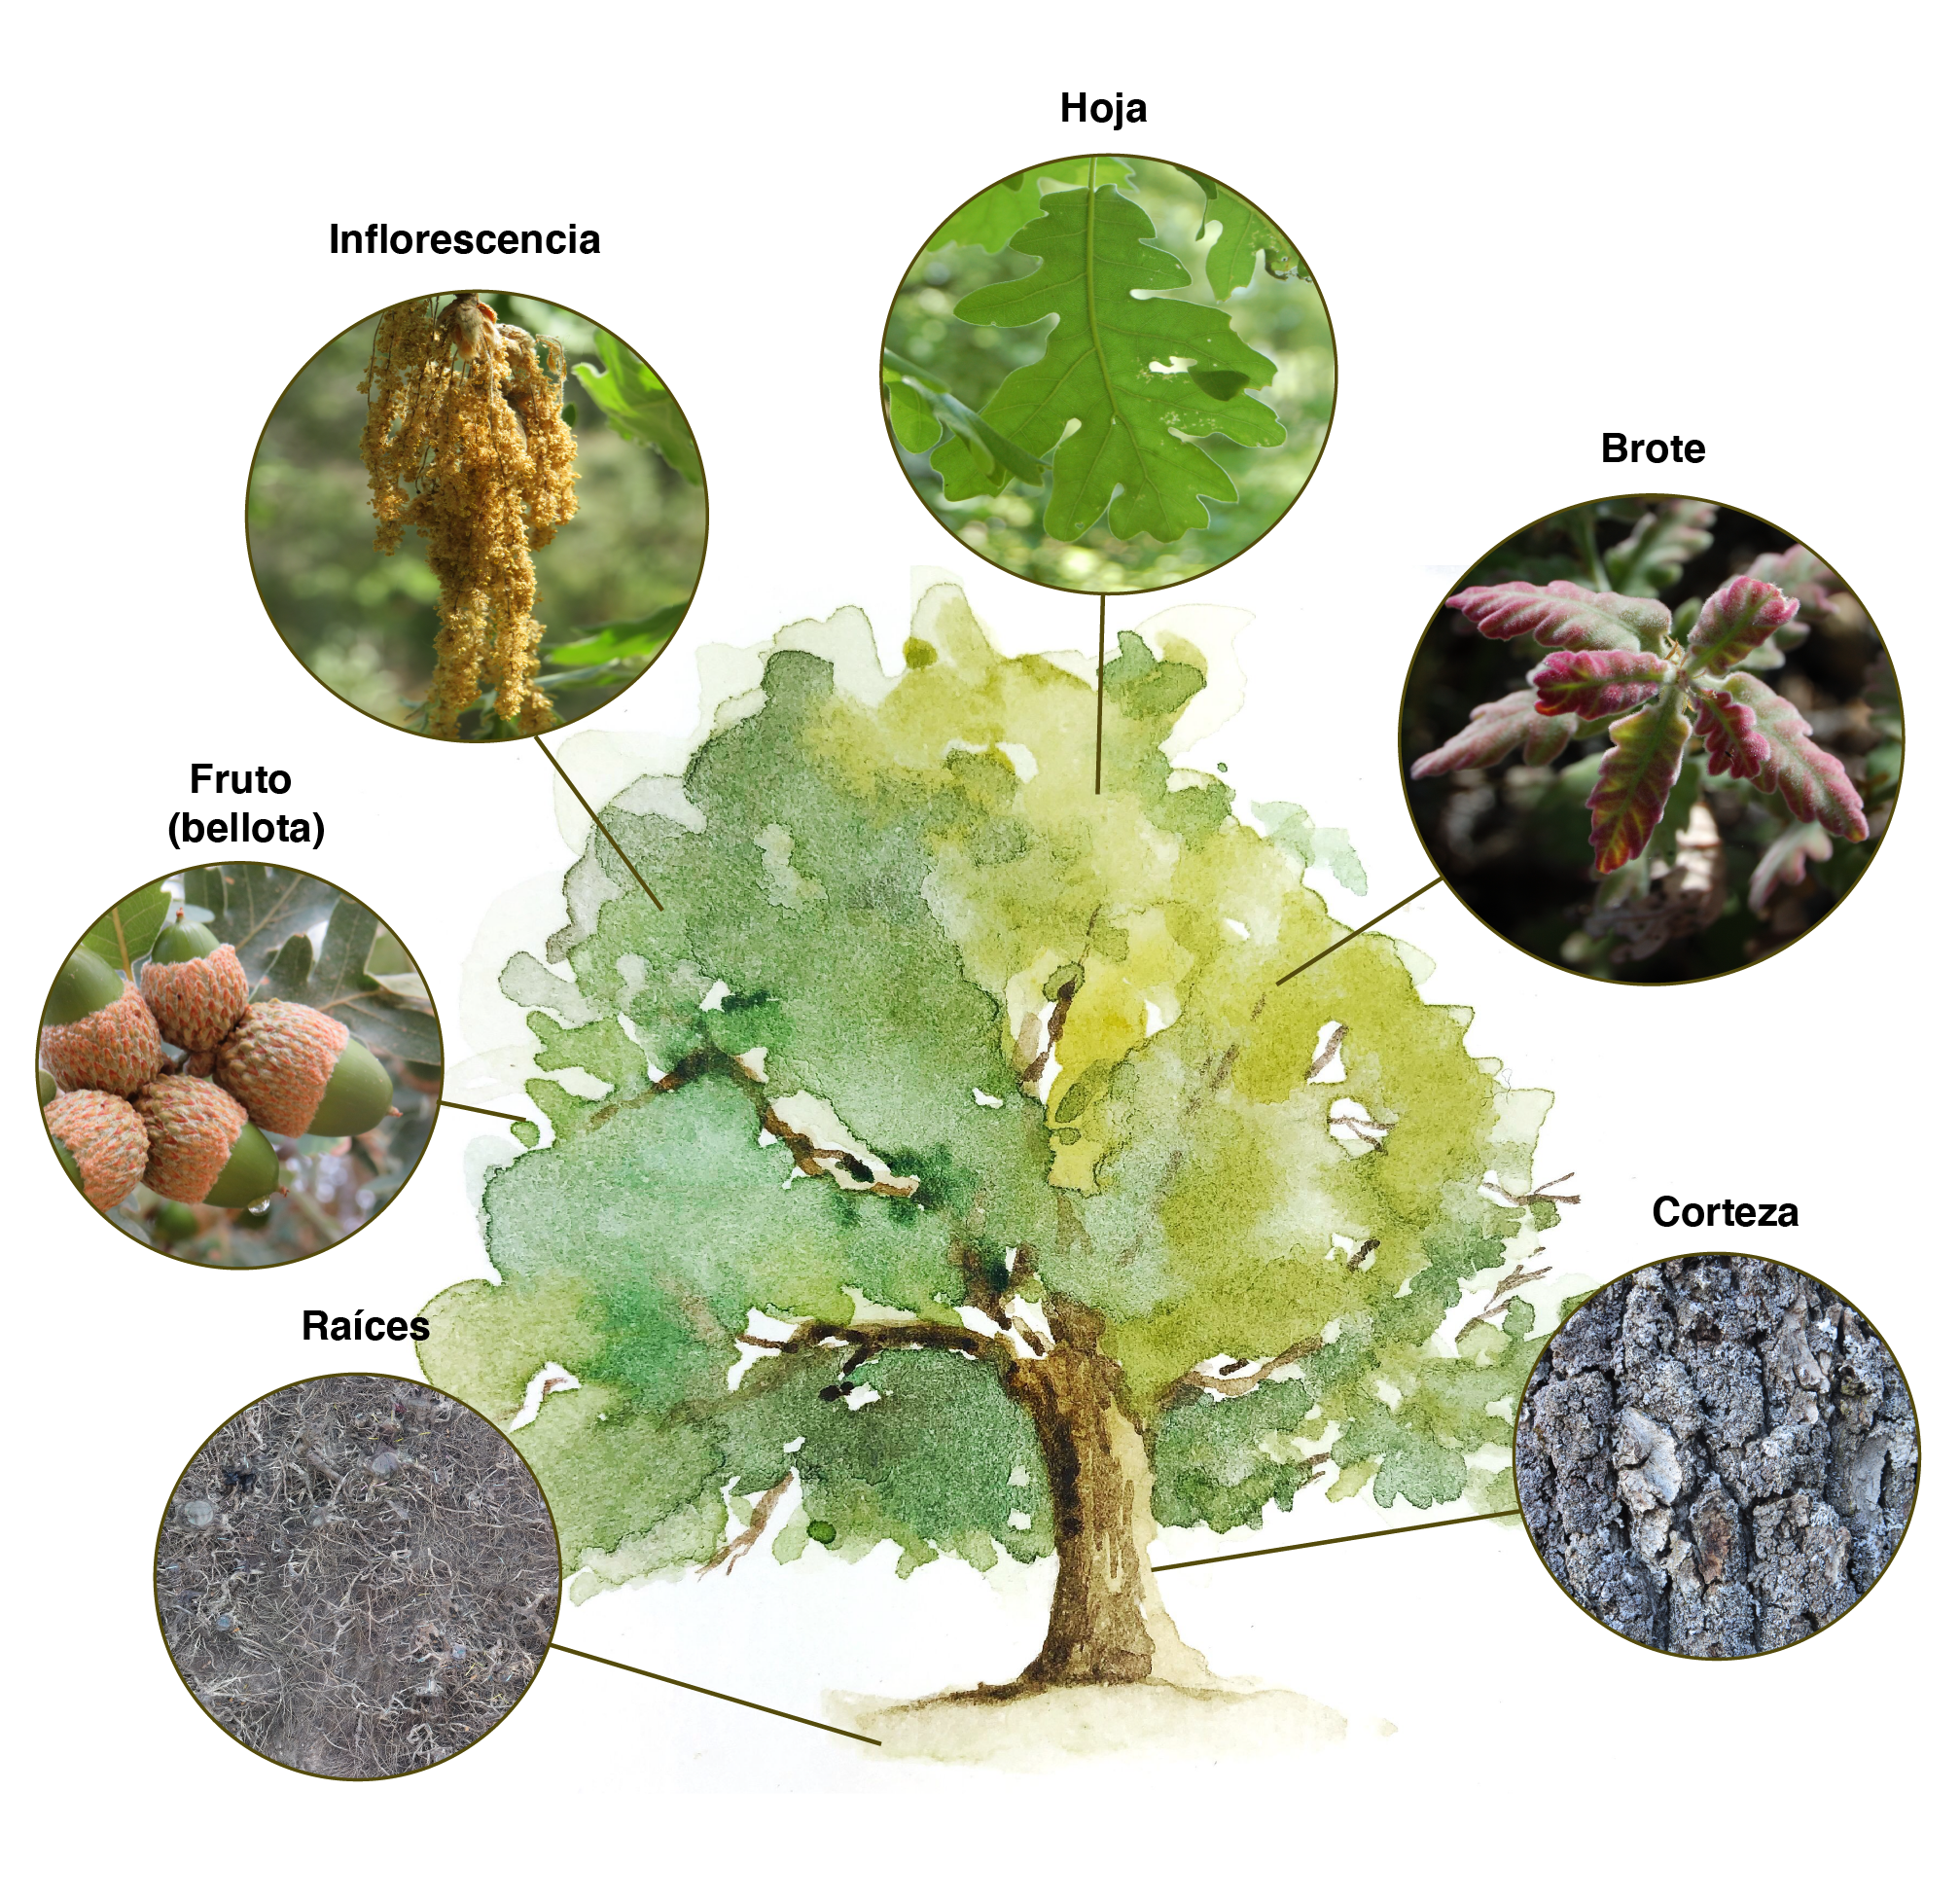
\includegraphics[width=\textwidth]{img/metodologia/metodologia-features-qp.png} \caption{Características del roble melojo (\Qpw). Fotos: M. Iglesias (raíces); A.J. Pérez-Luque.} \label{fig:metodologia:features-qp}
\end{figure}

Los robledales de roble melojo o melojares son formaciones dominadas por \Qpw que se distribuyen desde el suroeste de Francia hasta el noreste de Marruecos, ocupando su mayor extensión en la Península Ibérica, donde abarcan una amplia variedad de sitios y nichos ecológicos (\figreft{fig:metodologia:distroble}) \autocites{NietoQuintanoetal2016QuercusPyrenaica, GarciaJimenez20099230Robledales,VilchesdelaSerna2014ComprehensiveStudy,delaSernaetal2016MarcescentQuercus}. Según el Inventario Forestal Nacional \autocite{Villanueva2005TercerInventario}, estas formaciones ocupan 845 511 ha, lo que supone aproximadamente el 5\% de la superficie forestal de España. 

\begin{figure}[h]
	\centering
	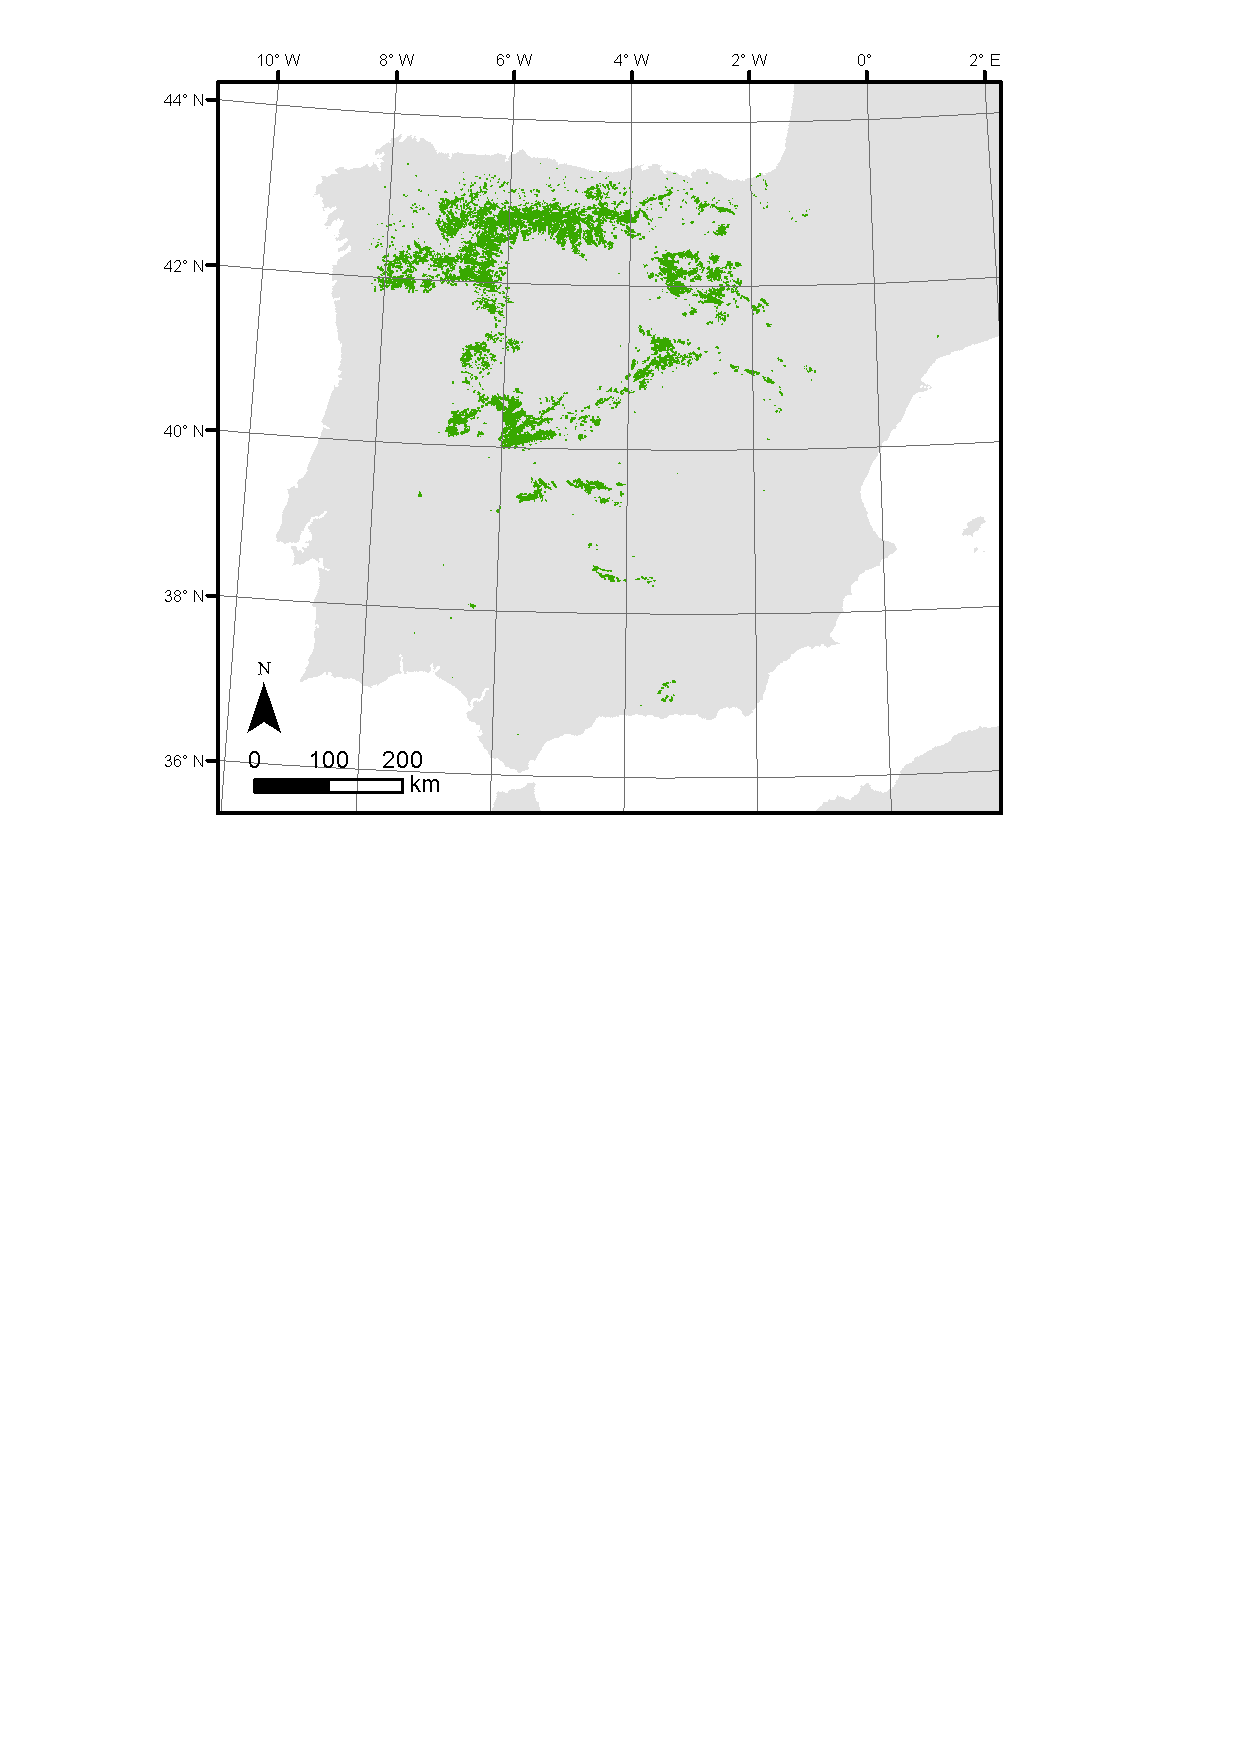
\includegraphics[width=0.75\textwidth]{img/metodologia/metodologia-robledal-spain-v2.pdf} \caption{Distribución de los bosques de \Qpy en la Península Ibérica. Elaboración propia a partir del Mapa Forestal Español} \label{fig:metodologia:distroble}
\end{figure}

Esta especie requiere de un mínimo de humedad estival para sobrevivir, que algunos autores han estimado en al menos 100 mm de precipitación entre mayo y agosto \autocite{BlancoCastroetal2005BosquesIbericos, Prieto1975BosquesSierra}. En Sierra Nevada el aporte extra de humedad necesario proviene de dos vías: de los ríos y acequias de careo, o del aire húmedo proveniente del Mediterráneo \autocites{PrietoEspinosa1977AestisilvaSierra, MartinezParrasMoleroMesa1982EcologiaFitosociologia,PerezRayaetal1990VegetacionSierra}. En efecto, los melojares en Sierra Nevada aparecen en aquellos enclaves más húmedos y de menor índice de insolación, principalmente barrancos y fondos de valle donde se dan unas condiciones microclimáticas favorables, tal y como ocurre en la zona occidental en orientaciones norte (ríos Alhama de Lugros, Maitena, Vadillo, Genil, Monachil, Dílar y Dúrcal) (\figreft{fig:metodologia:disposicion}a); o situados ocupando una determinada altura en la vertiente sur (Alpujarras: loma de Cáñar, barranco del Poqueira, loma de Pitres-Busquístar) en donde actúan como una banda de vegetación que intercepta la humedad procedente del Mediterráneo \autocites{Lorite2001VegetacionSierra,PrietoEspinosa1977AestisilvaSierra} (\figreft{fig:metodologia:disposicion}b). Estas diferencias también tienen reflejo en la composición florística de las poblaciones de ambas vertientes \autocites{Loriteetal2008PhytosociologicalReview,MelendoValle2000EstudioComparativo}.  

\begin{figure}
	\centering
	\includegraphics[width=\textwidth]{img/metodologia/metodologia-disposicionSN.pdf}\caption{Disposición de las poblaciones de robledal en la cara norte (\emph{e.g.} Robledal del valle del Río Genil)(\textbf{a}) y sur (\emph{e.g.} Robledal de Cáñar)(\textbf{b}) de Sierra Nevada. Modificado a partir de \citet{PrietoEspinosa1977AestisilvaSierra}.} \label{fig:metodologia:disposicion}
\end{figure}

\section{Área de estudio}
\label{sec:metodologia:sn}

Sierra Nevada es una región montañosa situada en el sur de Europa, que ocupa más de 2 000 km\textsuperscript{2} (\figreft{fig:metodologia:mapa-sn}). Presenta un rango altitudinal que varía entre 860 y 3 482 \elev, incluyendo la cumbre más alta de la Península Ibérica (Mulhacén). El clima es mediterráneo, caracterizado por inviernos fríos y veranos calurosos, con una pronunciada sequía estival. La temperatura media anual desciende en altitud desde los 12-16ºC por debajo de los 1 500 \elev hasta los 0ºC por encima de los 3 000 \elev de altitud. La precipitación media anual es muy irregular, con valores que oscilan entre los 250 y los 700 mm anuales, dependiendo  principalmente de la altitud y de la compleja orografía \autocites{PeinoCalero2020AnalisisVariabilidad, PerezLuqueetal2021ClimaNevadaBase}. Las precipitaciones invernales son principalmente en forma de nieve por encima de los 2 000 \elev de altitud \autocite{PerezPalazonetal2015ExtremeValues}. Geológicamente, la zona central está compuesta por rocas silíceas, principalmente micaesquistos, rodeadas de calizas y dolomías \autocite{RodriguezFernandez2017ParqueNacional}. Esta región montañosa alberga un total de 2 353 taxones de plantas vasculares, representando el 33\% y el 20\% de la flora de España y de Europa respectivamente \autocite{Lorite2016UpdatedChecklist}. Además presenta una alta tasa de endemicidad con 95 taxones vegetales endémicos \autocites{Loriteetal2007EstimationThreatened,Loriteetal2020FloraSNevadaTrait}. La cubierta forestal de Sierra Nevada está dominada por plantaciones de pino (\emph{Pinus halepensis} Mill., \emph{P. pinaster} Ait., \emph{P. nigra} Arnold subsp. \emph{salzmannii} (Dunal) Franco, y \emph{P. sylvestris} L.) que cubren aproximadamente 37 000 ha. Los bosques autóctonos están dominados principalmente por la encina (\emph{Quercus ilex} subsp. \emph{ballota} (Desf.) Samp.) ocupando zonas de baja y media montaña (11 000 ha) y el roble melojo (\Qpw) que va desde los 1 100 a los 2 000 \elev, cubriendo unas 3 400 ha \autocites{Lorite2001VegetacionSierra, PerezLuqueetal2019MapEcosystems}.

\begin{figure}
	\centering
	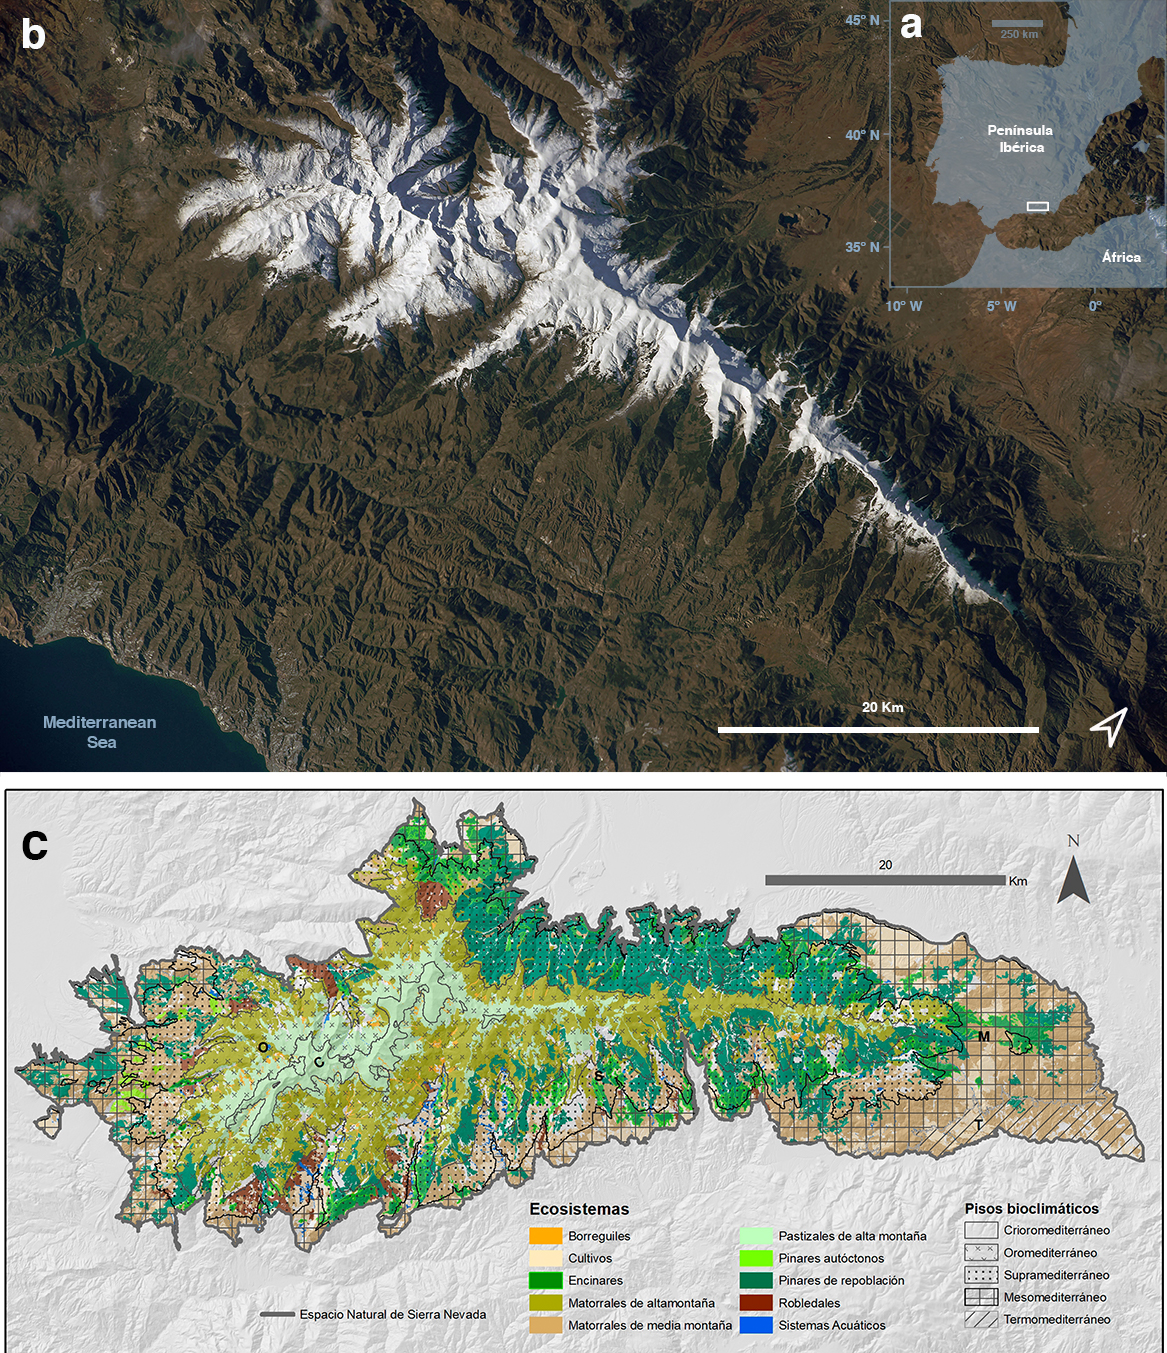
\includegraphics[width=0.99\textwidth]{img/metodologia/metodologia-mapasn.jpg}
	\caption{Localización (\textbf{a}) y vista de satélite de Sierra Nevada (\textbf{b}). Distribución espacial de los ecosistemas de Sierra Nevada  (\textbf{c}). Se indican los pisos bioclimáticos. Imagen de la Estación Espacial Internacional tomada en diciembre de 2014; cortesía de \emph{Earth Science and Remote Sensing Unit, NASA Johnson Space Center}.}\label{fig:metodologia:mapa-sn}
\end{figure}


Sierra Nevada contiene 27 hábitats tipo incluidos en la Directiva Hábitats, 28 especies de aves del Anexo I de la Directiva Aves y 15 especies de animales incluidas en el Anexo II de la Directiva Hábitats (1 reptil, 2 anfibios, 7 mamíferos y 5 invertebrados). Todo ello hace que esté considerada como uno de los \emph{hotspots} de biodiversidad más importantes en la Región Mediterránea \autocites{Blanca1996ProteccionFlora,Blancaetal1998ThreatenedVascular,MedailQuezel1999BiodiversityHotspots,Canadasetal2014HotspotsHotspots}. En Sierra Nevada hay 61 municipios con un total de mas de 90 000 habitantes, siendo sus principales actividades económicas la agricultura, el turismo, la ganadería, la apicultura, la minería, y el esquí \autocite{FernandezMarquezSalinas2009ImpactoSocioeconomico}. El alto valor de biodiversidad y geodiversidad, así como su riquerza paisajística y cultural han hecho que Sierra Nevada presente varios reconocimientos y cuente con diversas figuras legales de protección. Además de contar con un Parque Nacional y un Parque Natural, Sierra Nevada es una Reserva de la Biosfera (MaB, Unesco). Está incluida en la red Natura 2000 como Zona de Especial Protección para las Aves y Lugar de Interes Comunitario (LIC). 

Una de las características más importantes de Sierra Nevada es la existencia de marcados gradientes altitudinales, ecológicos y climáticos \autocite{Zamoraetal2021UniendoMacro}. Así por ejemplo, existe un fuerte contraste climático entre las laderas soleadas y secas orientadas al sur, y las laderas sombreadas y más húmedas orientadas al norte. La heterogeneidad climática y topográfica existente en Sierra Nevada ofrece una gran diversidad de microhábitats, lo que ha permitido a esta región montañosa actuar como refugio de diferentes especies \autocites{MedailDiadema2009GlacialRefugia,GomezLunt2007RefugiaRefugia,BlancoPastoretal2019TopographyExplains}, incluyendo especies caducifolias de \emph{Quercus} durante la última glaciación \autocites{Olaldeetal2002WhiteOaks,RodriguezSanchezetal2010TreeRange,Petitetal2002IdentificationRefugia}. 

La existencia de estos gradientes confiere a Sierra Nevada, y a las regiones montañosas en general, el carácter de un excepcional laboratorio natural de seguimiento del cambio global \autocite{Zamora2010AreasProtegidas,Zamoraetal2017MonitoringGlobal}. De hecho, en 2008 se estableció el Observatorio de Cambio Global de Sierra Nevada (OBSNEV) (https://obsnev.es), un programa de seguimiento a largo plazo para evaluar el impacto del cambio global en los ecosistemas nevadenses \autocites{Aspizuaetal2010ObservatorioCambio,BonetGarciaetal2011SierraNevada}. Esta iniciativa está recopilando información útil y relevante sobre los efectos del cambio global en los sistemas socieoecológicos de Sierra Nevada \autocites{Zamoraetal2015HuellaCambio,Zamoraetal2017GlobalChange,PerezLuqueetal2016SenalesCambio, RamosLosadaetal2017TenYears}. Asimismo, y relacionado con la temática de la presente memoria doctoral, dentro de las metodologías de seguimiento de esta iniciativa, se vienen realizando diferentes análisis sobre los efectos del cambio global en las masas de robledal \autocites[ver por ejemplo][]{BonetGarciaetal2015ImpactosCambio,Aspizuaetal2012EvaluacionGestion,Munoz2012BosquesAutoctonos}. 

\subsubsection{Melojares en Sierra Nevada}
\label{sec:metodologia:qpsn}

En Sierra Nevada, los melojares ocupan actualmente una extensión de 3 400 ha \autocite{PerezLuqueetal2019MapEcosystems}, distribuidas entre los 1 000 y 2 000 \elev, y situados exclusivamente sobre suelos silíceos. 
Aunque representan menos del 7\% de la superficie forestal existente en Sierra
Nevada (\figreft{fig:metodologia:mapa-sn}c), tienen una alta singularidad ecológica y presentan una alta diversidad de especies vegetales en comparación con las otras formaciones forestales \autocite{GomezAparicioetal2009ArePine,PerezLuqueetal2014SinfonevadaDataset}. Además, albergan diferentes especies vegetales consideradas relictas \autocite{Loriteetal2008PhytosociologicalReview, Blancaetal1998ThreatenedVascular} (Ver apéndice \ref{sec:appendix:multivar}). 

\section{Análisis del patrón de colonización de cultivos abandonados}\label{sec:metodologia:coloniza}

En el capítulo \ref{sec:coloniza} se estudia el patrón de colonización de los cultivos de montaña abandonados. La aproximación que utilizamos consistió en el estudio de los diferentes módulos implicados en la dispersión \autocite[][]{LundbergMoberg2003MobileLink,Nathanetal2012DispersalKernels}, a saber: fuente semillera (bosques de \Qpy); vector de dispersión (animales dispersores de bellotas); y  sumidero receptor de semillas (cultivos abandonados).

Se seleccionaron 5 cultivos abandonados situados en dos localidades de Sierra Nevada que representan las dos vertientes: robledal de San Juan (Robledal del río Genil; oientación NW); y robledal de Cáñar (orientación sur). Para cada uno de los cultivos abandonados, se llevó a cabo un análisis de la estructura forestal circundante y del patrón de regeneración. Para ello se  distribuyeron al azar transectos lineales de vegetación (30x10 m) en el cultivo abandonado; en los bordes del bosque y dentro de los bosques circundantes (\figreft{fig:metodologia:coloniza}). El número de transectos en cada uno de los cultivos abandonados fue proporcional al tamaño de los campos de cultivo abandonado (ver \tabreft{tab:coloniza:croplands}). 

En cada transecto de vegetación se registraron todos los individuos y se midió la altura y el diámetro de los mismos (diametro base para individuos con altura \textless 150 cm; y diámetro a la altura del pecho para individuos con altura \textgreater 150 cm). Para cada transecto se calculó la abundancia de juveniles, sin diferenciar entre regeneración vegetativa y sexual debido a la dificultad que presenta la especie por su carácter rebrotador. Dentro de los juveniles se diferenciaron varias etapas de reclutamiento en función del tamaño de los individuos \autocite[\emph{e.g.}][]{Plieningeretal2010LargeScalePatterns}. Consideramos cinco categorías de tamaño basadas en la altura (cada 30 cm). 

\begin{figure}
    \centering
    \includegraphics[width=0.8\textwidth]{img/metodologia/metodologia-coloniza.pdf}
    \caption{Esquema metodológico de análisis del patrón de colonización de cultivos. Se estudió la estructura de la fuente semillera (1), el estado de la comunidad de arrendajos (el principal dispersor de bellotas)(3), y la regeneración observada en los cultivos abandonados (2)}
    \label{fig:metodologia:coloniza}
\end{figure}

Para estudiar la comunidad de dispersantes se utilizó una serie temporal de datos de abundancia del arrendajo (\emph{Garrulus glandarius}), el principal dispersor de las bellotas de \Qpy en Sierra Nevada \autocite[][]{Gomez2003ImpactVertebrate}. Esta serie de datos procede del seguimiento de aves paseriformes realizado en el marco del Observatorio de Cambio Global de Sierra Nevada \autocites{Zamoraetal2017MonitoringGlobal,BareaAzconetal2012PasseriformesOtras}. En concreto se utilizaron datos para los robledales de la zona de estudio (Robledal de Cáñar y Robledal de San Juan). Estos muestreos consistieron en censos realizados a lo largo de transectos lineales con un ancho de banda fijo de 50 m (25 a cada lado del observador), en donde se registraron todos los avistamientos \autocites{BareaAzconetal2012PasseriformesOtrasa, ZamoraBareaAzcon2015LongTermChanges}. 

Todos los datos fueron debidamente documentados y publicados en repositorios institucionales: véase \citet{PerezLuqueetal2015DatasetMIGRAME} para una descripción detallada del conjunto de datos de los transectos de vegetación; y \citet{PerezLuqueetal2016DatasetPasserine} para la descripción del conjunto de datos sobre aves paseriformes. 

\section{Estimación de biomasa a nivel de parcela}\label{sec:metodologia:biomasa}

En el capítulo \ref{sec:carbon} se llevó a cabo una estimación de la biomasa utilizando ecuaciones alométricas \autocite[ver][]{Monteroetal2005ProduccionBiomasa} a partir de datos de inventarios forestales. Los datos de campo se obtuvieron a partir de una recopilación de varios inventarios forestales y proyectos de investigación realizados en Sierra Nevada. En primer lugar, se seleccionaron las parcelas incluidas en la distribución actual de \Qp en Sierra Nevada \autocite{PerezLuqueetal2019MapEcosystems}. A continuación se seleccionaron únicamente las parcelas con información completa (aquellas en las que se midieron todos los individuos arbóreos con DBH \textgreater{} 7,5 cm), y los rodales puros (composición \textgreater{} 70\%). De estas parcelas, se aplicó un filtro espacial para descartar las parcelas superpuestas, y un filtro temporal, descartando los inventarios de antiguos (es decir, de más de 10 años). Todas las parcelas seleccionadas se midieron entre 2012 y 2020. 

Además de ello, y para tener una representación de todas las poblaciones de robledal, se muestrearon parcelas circulares adicionales (de 9 a 16 m de radio) entre octubre de 2019 y marzo de 2020. En cada parcela se marcaron y midieron todos los ejemplares arbóreos. Se anotó el diámetro a la altura del pecho (DBH) utilizando un calibre forestal graduado (precisión de 0.1 cm). La altura de cada árbol se midió utilizando un hipsómetro (Vertex 5, Haglöf Sweden) con una precisión de 0.1 metros. También se anotó para cada ejemplar el azimut y la distancia respecto al centro de la parcela, cuya posición fue registrada mediante la utilización de un GPS submétrico (Leica Zeno 20 GIS, Leica Geosystems, Suiza). Las parcelas se seleccionaron en proporción a la extensión de los diferentes estratos ecológicos, proporcionando rodales representativos con una variedad de estructura de rodal y condiciones de sitio en las diferentes poblaciones de robledal de Sierra Nevada. 

\section{Muestreos dendrocronológicos}
\label{sec:metodologia:dendro}

En el capítulo \ref{sec:dendro}, realizamos una estimación del crecimiento secundario de los robledales, para lo cual llevamos a cabo muestreos dendrocronológicos estándar para obtener series de crecimiento radial \autocite{Fritts1976TreeRings,CookKairukstis1990MethodsDendrochronology,Gutierrez2008DendrocronologiaMetodos,Natalinietal2017TecnicasHerramientas}.

En cada sitio de muestreo (Robledal del Genil, GEN; y Robledal de Cáñar, CAN; ver capítulo \ref{sec:dendro}), se seleccionaron entre 15 y 20 árboles de forma aleatoria. Para cada árbol focal (\emph{target tree}), se tomaron entre 2-3 testigos (\emph{cores}) de 5 mm de diámetro utilizando una barrena forestal o barrena de Pressler \autocite{GrissinoMayer2003ManualTutorial} (\figreft{fig:metodologia:barrena-gente}). Los testigos se tomaron de forma perpendicular, y a una altura de 1.3 metros (\figreft{fig:metodologia:cores-combina}b). Cada testigo se etiquetó y se guardó en pajitas (preferiblemente de papel) para su transporte. Posteriormente en el laboratorio, los testigos se secaron al aire, y se montaron en soportes de madera para su posterior lijado y análisis (\figreft{fig:metodologia:cores-combina}b-c). Durante el montaje, los testigos se colocaron de tal forma que las fibras quedaran perpendiculares a la superficie de lectura, y dejando visible la sección transversal, facilitando así la observación de los anillos \autocite{Fritts1976TreeRings,Natalinietal2017TecnicasHerramientas}. Para el lijado de las muestras se utilizó una lijadora eléctrica usando papeles de lija de granos sucesivamente mas finos (desde 60 hasta 1200).

\begin{figure}
    \centering
    \includegraphics[width=0.8\textwidth]{img/metodologia/metodologia-barrena-gente.jpg}
    \caption{Obtención de testigos con Barrena de Pressler.}
    \label{fig:metodologia:barrena-gente}
\end{figure}

\begin{figure}
    \centering
    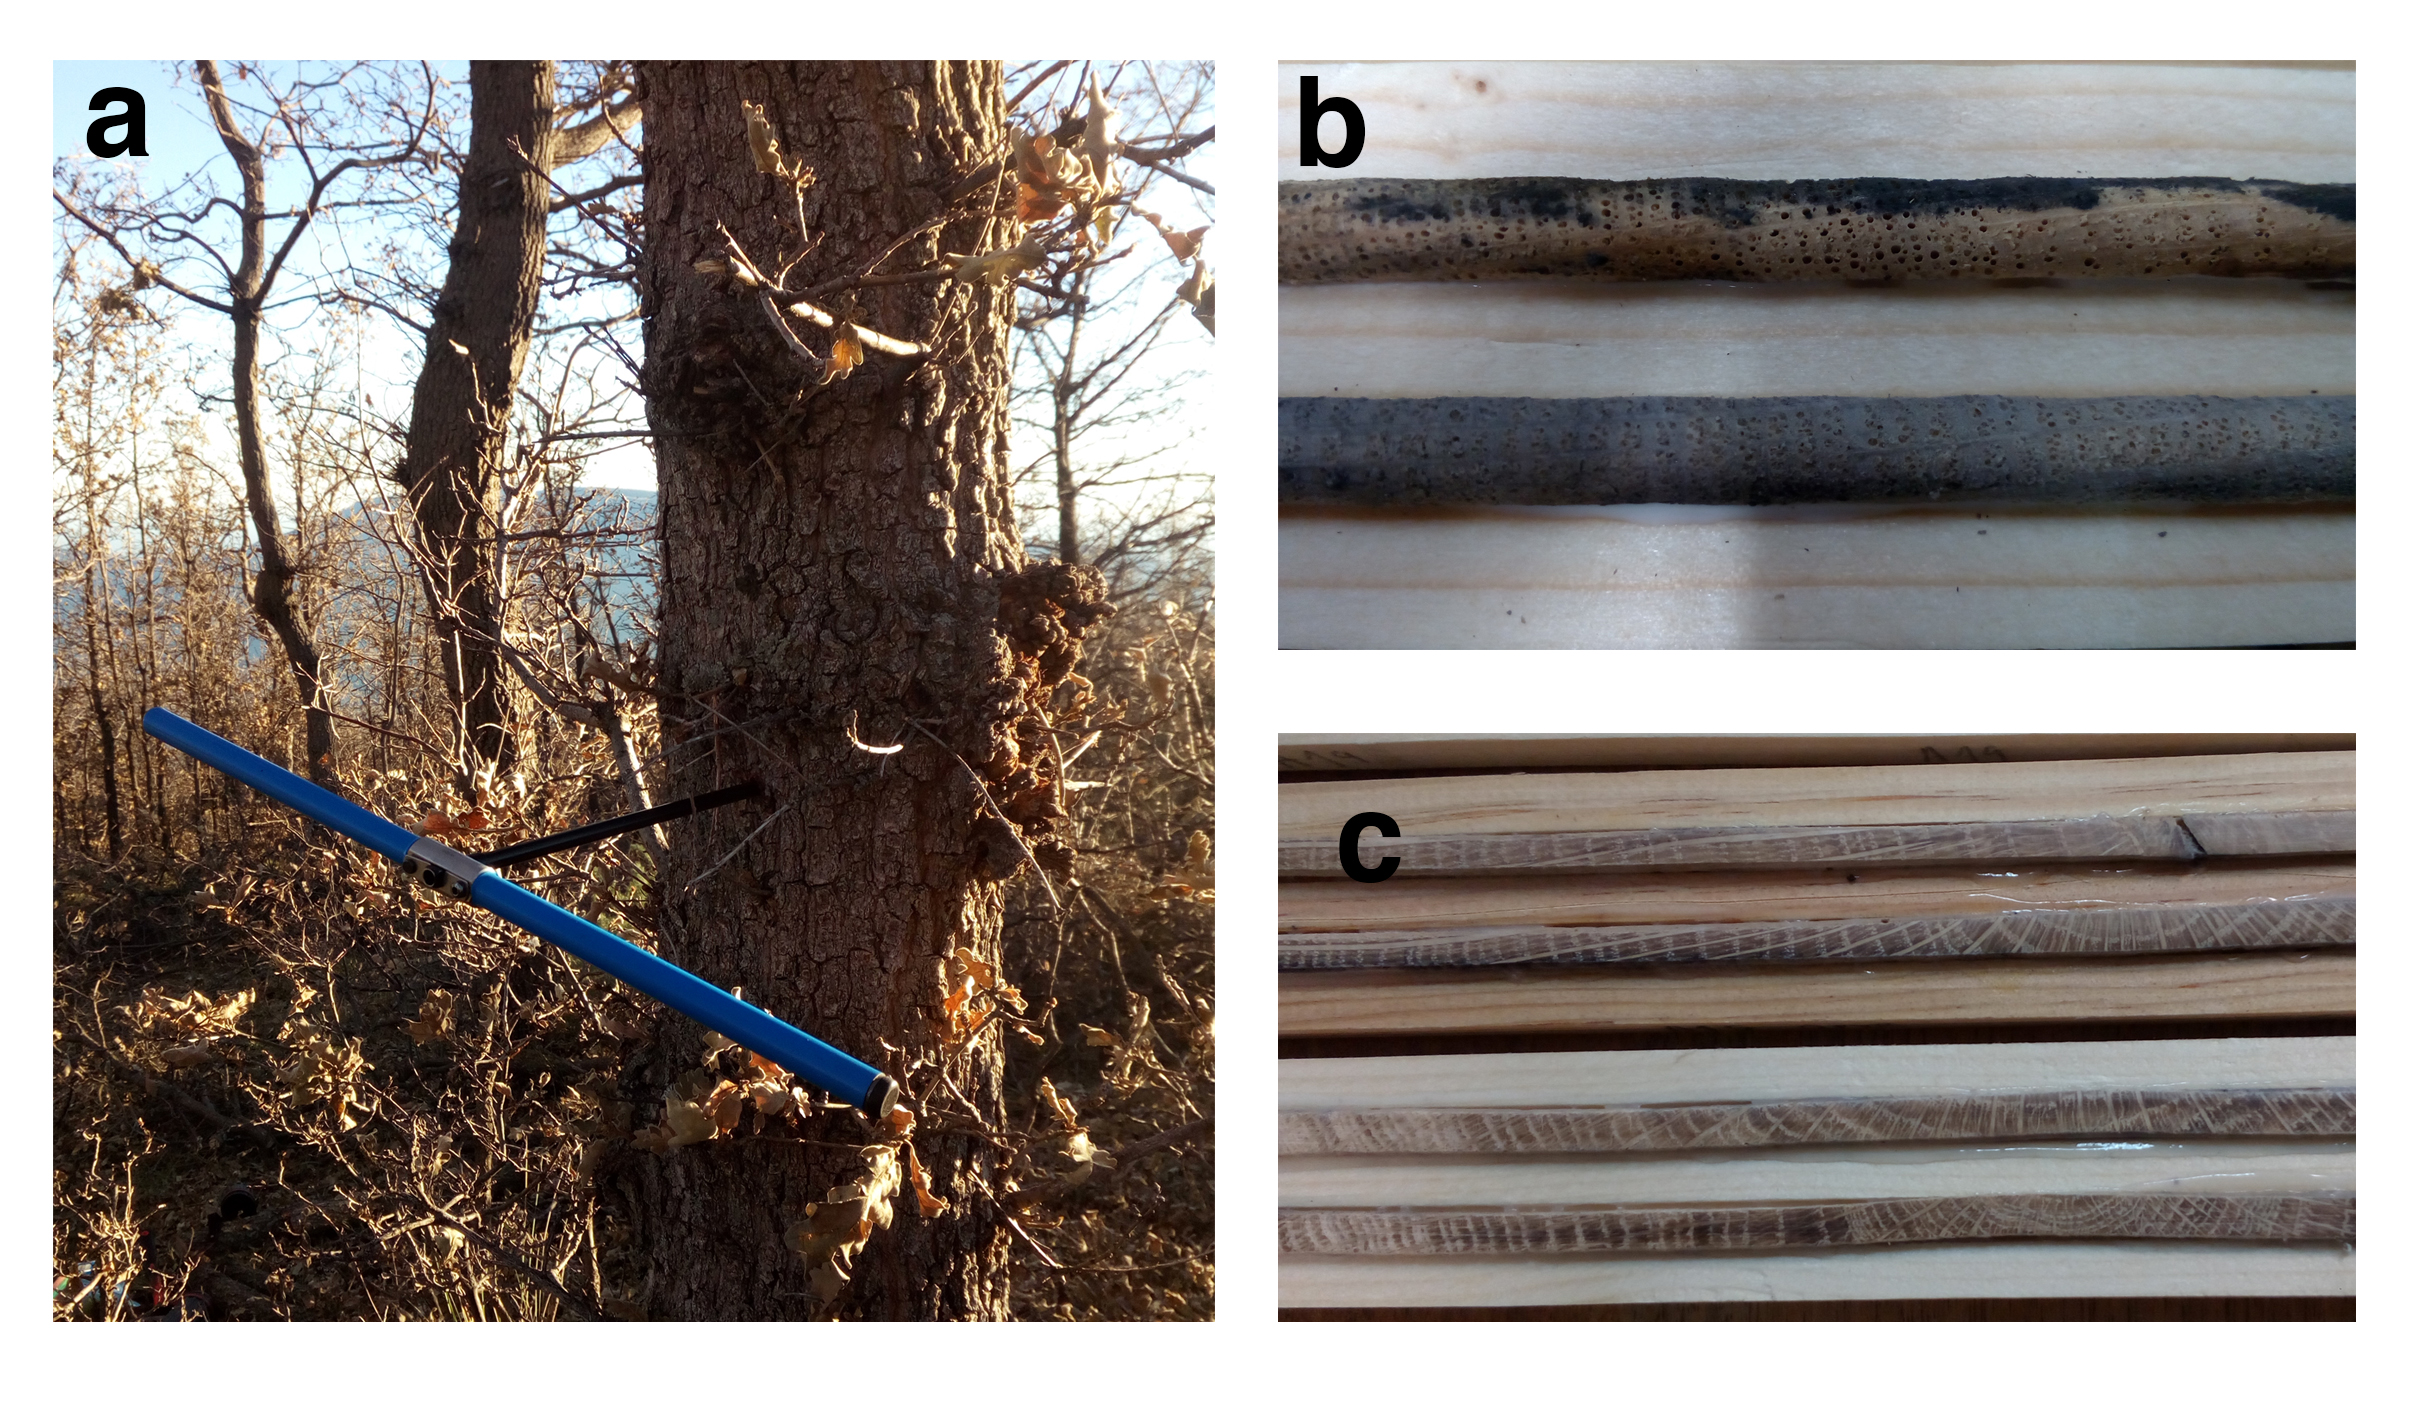
\includegraphics[width=0.99\textwidth]{img/metodologia/metodologia-cores-combina.jpg}
    \caption{Barrena de Pressler (\textbf{a}) obteniendo testigos de un ejemplar de \Qpy. Testigos montados sobre soporte de madera, antes (\textbf{b}) y después (\textbf{c}) de ser lijados.}
    \label{fig:metodologia:cores-combina}
\end{figure}

Posteriormente se procedió a la medición, desde la corteza hasta la médula, de la anchura de todos los anillos de crecimiento (\emph{RW}, \emph{ring width}) con una precisión de 0.01 mm, utilizando una mesa de medición LINTAB acoplada a un estereomicroscopio de alta resolución y a un ordenador con el software TSAP-Win (Rinntech, Heidelberg, Alemania). Una vez realizadas las mediciones, las series se sincronizaron visualmente y se dataron utilizando los estadísticos \emph{Gleichläufigkeit} (GLK), \emph{t-valor} e índice de datación cruzada (\emph{CDI}, \emph{crossdate index}) \autocite{Schweingruber1988TreeRings,BurasWilmking2015CorrectingCalculation}. Se sincronizaron los testigos pertenecientes al mismo árbol entre sí, construyeron cronologías de individuo, para posteriormente generar cronologías de sitio. La datación cruzada visual se verificó utilizando el programa COFECHA, que calcula la intercorrelación entre series mediante segmentos solapados \autocite{Holmes1983ComputerassistedQuality}. Este programa ayuda a evaluar la calidad de la datación cruzada y a identificar posibles problemas dentro de una serie de anillos de crecimiento \autocite{GrissinoMayer2001EvaluatingCrossdating}.

\subsection{Estimación de la competencia}
\label{sec:metodologia:competencia}
Para la estimación de la competencia de cada árbol focal (\emph{target tree}) se emplearon diferentes \textbf{índices de competencia}. La mayoría de los índices de competencia descritos en la literatura forestal pueden dividirse en dos grandes clases: los \emph{índices independientes de la distancia}, que utilizan únicamente información no espacial sobre el tamaño y el número de árboles agregados dentro de un área determinada (\emph{e.g.} una parcela o un rodal); y los \emph{índices dependientes de la distancia} que además incorporan las ubicaciones relativas de los árboles vecinos dentro del área \autocite{Contreras2011,GeaIzquierdoCanellas2009AnalysisHolm,BurkhartTome2012IndicesIndividualtree}. Los índices dependientes de la distancia, aunque son mas tediosos de obtener, presentan una mejor correlación con el crecimiento que los índices independientes de la distancia \autocites{GeaIzquierdoCanellas2009AnalysisHolm,Contreras2011,Maleki2015}. En nuestro caso empleamos los índices independientes de la distancia, \emph{densidad} ($n \\; árboles \cdot ha^{-1}$) y \emph{área basal} ($m^{2} \cdot ha^{-1}$); así como el índice dependiente de la distancia \emph{ratio de tamaños proporcional a la distancia} (\emph{srd}, del inglés \emph{size ratio proportional to distance}) calculado como \[\mathrm{srd} = \sum_{i=1}^{n} ( \frac{dbh_j}{dbh_i}) \times \left[\frac{1}{(dist_{ij} + 1)} \right]\]
siendo \(dbh_i\) y \(dbh_j\) los diámetros a la altura del pecho del árbol $i$ y el árbol focal ($j$) respectivamente; y \(dist_{ij}\) la distancia entre ambos árboles.

Se muestrearon todos los árboles vivos con DBH \textgreater{} 7.5 cm dentro de una parcela circular de 10 m de radio, tomando como centro el árbol focal. Para cada árbol, se anotó la especie, se midió la altura y el DBH, así como la distancia y ángulo (\emph{azimuth}) respecto al árbol focal (\figreft{fig:metodologia:competence}).


\begin{figure}
	\centering
	\includegraphics[width=0.99\textwidth]{img/metodologia/metodologia-competence.pdf}
	\caption{
	Esquema de los muestreos para estimación de la competencia (\textbf{a}). Se replantean parcelas de 10 m de radio en torno al árbol focal. Cada árbol vecino es identificado (\textbf{b}) y medido (\textbf{c}), anotando la distancia y azimuth respecto al centro, así como su altura y DBH.}\label{fig:metodologia:competence}
\end{figure}

\section{Índices de Vegetación}\label{sec:metodologia:modis-iv}

La información derivada de las imágenes de satélite (teledetección) proporciona un medio relativamente barato y accesible para obtener series temporales de información, a distintas escalas espaciales, sobre
diferentes atributos de los ecosistemas, lo que supone un gran potencial para el seguimiento de los cambios en el funcionamiento de los escosistemas \autocites{Pettorellietal2014SatelliteRemote,Pettorellietal2018SatelliteRemote,Cabelloetal2012EcosystemFunctioning, Alcarazetal2006IdentificationCurrent,AlcarazSeguraetal2015CambiosProductividad}.

Los índices de vegetación (\emph{IV}) son los índices espectrales derivados de imágenes de satélite más utilizados. Estos índices se pueden utilizar para estimar la fracción de la radiación fotosintéticamente activa absorbida por la vegetación (fPAR), que representa el control principal de la producción primaria
\autocite{Monteith1972SolarRadiation}, debido a la relación lineal existente entre ambas variables \autocites{Hatfieldetal1984InterceptedPhotosynthetically}. Gracias a la relación con la productividad primaria neta, los índices de vegetación se han empleado para derivar indicadores del funcionamiento ecosistémico, tales como el carbono total anual absorbido por la vegetación, o la estacionalidad y fenología de la dinámica de las ganancias de carbono \autocites{CabelloParuelo2009TeledeteccionEstudios,
AlcarazSeguraetal2009BaselineCharacterization,AlcarazSeguraetal2009UseDescriptors,Cazorlaetal2020RemoteSensingbased,Dionisioetal2012SatelliteBasedMonitoring}. En el marco de la presente memoria doctoral se utilizaron los índices \textbf{EVI}, Índice de Vegetación Mejorado (\emph{Enhanced Vegetation Index}) (ver capítulo \ref{sec:dendro}) y
el \textbf{NDVI}, Índice de Vegetación de Diferencia Normalizada (\emph{Normalized Difference Vegetation Index}) (capítulo \ref{sec:onto}). A partir de las series temporales construidas para cada índices, se obtuvieron
diferentes indicadores sintéticos de la dinámica de la intercepción de radiación por parte de la vegetación, tales como el promedio anual y estacional, la estacionalidad o la fenología del ecosistema, con los
que, posteriormente caracterizar y monitorear diferentes aspectos del funcionamiento de los ecosistemas
\autocite{Cabelloetal2012EcosystemFunctioning}.

El NDVI es un índice espectral que tiene en cuenta la diferente absorción de la radiación solar por parte de la vegetación en las bandas del rojo (\emph{red}) e infrarrojo (\emph{NIR}) cercano dentro del espectro electromagnético. Su valor se computa como \[NDVI = \frac{\rho_{NIR} - \rho_{red}}{\rho_{NIR} + \rho_{red}}\],

siendo \(\rho_{NIR}\) y \(\rho_{red}\) las reflectacias de las bandas infrarrojo cercano (NIR) y rojo respectivamente. Al tratarse de un índice normalizado, sus límites teóricos son -1 y 1, representando a la
vegetación los valores superiores a cero \autocites{Hueteetal2002OverviewRadiometric}. El EVI, por su parte, es un índice espectral que tiene en cuenta la diferente absorción de la radiación solar por parte de la vegetación en las bandas del rojo e infrarrojo cercano (además de incluir la banda del azul como corrección)
dentro del espectro electromagnético \autocites{Hueteetal2002OverviewRadiometric}. Su fórmula además incorpora una serie de constantes para corregir ciertos efectos de la atmósfera y el suelo:
\[EVI = G\times\frac{(\rho_{NIR}-\rho_{red})}{\rho_{NIR} + C_{1} \times \rho_{red} - C_{2}\times \rho_{blue} + L}\]
siendo \(\rho_{NIR}\), \(\rho_{red}\), y \(\rho_{blue}\) las reflectacias de las bandas infrarrojo cercano (NIR), rojo y azul respectivamente. \(L\) es el ajuste del fondo del dosel, \(C_{1}\) y \(C_{2}\) coeficientes de que corrigen la influencias de los aerosoles, y \(G\) el factor de ganancia. En el algoritmo de MODIS-EVI, los valores adoptados para esos coeficientes son: \(L = 1\); \(C_{1} = 6\) y \(C_{2}=7.5\) y \(G = 2.5\) \autocites{Hueteetal2002OverviewRadiometric}.

Las imágenes de EVI y NDVI fueron derivadas del producto MOD13Q1 obtenido por el sensor MODIS (\emph{Moderate Resolution Imaging Spectroradiometer}) \autocites{Didan2015MOD13Q1MODIS}. Estas imágenes tienen una resolución espacial de 231 m y temporal de 16 días (23 imágenes por año). Los datos de MODIS de la Colección 6 se obtuvieron utilizando la plataforma Google Earth Engine \autocites{Gorelicketal2017GoogleEarth}. Seleccionamos los píxeles que cubren la distribución de los bosques de \emph{Q. pyrenaica} en Sierra Nevada (\emph{n} = 928 píxeles). Posteriormente se aplicó un filtrado de datos para seleccionar los valores válidos de los índices de vegetación. El filtrado se realizó utilizando los indicadores de calidad (banda \emph{250m 16 days VI Quality}) que acompañan a cada imagen. A partir de esa información, filtramos aquellos valores afectados por alto contenido de aerosoles, nubes, nieve y sombras, siguiendo las recomendaciones de filtrado de datos de imágenes de satélite para regiones de montaña \autocites{ReyesDiezetal2015ImplicacionesFiltrado}.

Para cada uno de los índices, generamos series temporales desde 2000 hasta 2014 (NDVI) (capítulo \ref{sec:onto}) y 2016 (EVI) (capítulo \ref{sec:dendro}). De las series temporales generadas se derivaron los perfiles anuales (\figreft{fig:onto:indicator}) y se calcularon diferentes métricas (promedio anual, estacional, máximo, mínimo, etc) en función de las necesidades de estudio (ver capítulos \ref{sec:dendro} y \ref{sec:onto}). 

\section{Estimación de indicadores de la cubierta de nieve}\label{sec:metodologia:modis-nieve}
La producción primaria de la vegetación depende de multitud de factores biofísicos. En regiones de montaña como Sierra Nevada, la nieve puede jugar un papel determinante en este sentido. La cantidad de agua suministrada por la nieve puede explicar, en parte, el funcionamiento de ecosistemas forestales cercanos al límite del árbol. En el capítulo \ref{sec:onto} se evalúan las relaciones entre la duración de la cubierta de nieve y la productividad en los robledales de \emph{Q. pyrenaica}. Para ello, además de los índices de vegetación antes mencionados, se ha generado una serie temporal sobre la dinámica de la cubierta de nieve en
los robledales de Sierra Nevada \autocites{PerezLuqueetal2016TemporalTrend,BonetGarciaetal2015AnalisisTendencias}. A partir del producto MOD10A2 de MODIS \autocites{Halletal2002MODISSnowcover}, que presenta una periodicidad de 8 días y una resolución espacial de 500 m, se calculó el índice diferencial normalizado de nieve \textbf{NDSI} (\emph{Normalized Difference Snow Index}). Se trata de un ratio de bandas espectrales que aprovecha la mayor reflectancia de la nieve en las longitudes de onda visible, y baja reflectancia en la región infrarroja de onda corta
\autocites{SalomonsonAppel2006DevelopmentAqua} \[NDSI = \frac{\rho_{green} - \rho{SWIR}}{\rho_{green} + \rho{SWIR}}\]

siendo \(\rho_{green}\) y \(\rho{SWIR}\) las reflectancias en las bandas visible e infrarrojo de onda corta respectivamente. Este índice ha demostrado ser un indicador robusto de la cobertura de nieve utilizando
imágenes MODIS \autocites{Rittgeretal2013AssessmentMethods}. Se derivaron diferentes indicadores que caracterizan la cubierta de nieve \autocites{WangXie2009NewMethods}: 

\begin{itemize}
\item \emph{duración de la cubierta de
nieve} (\emph{scd}, \emph{snow cover duration}): se define como el número de días cubiertos de nieve por año hidrológico.
\item \emph{fecha de inicio de la cubierta de nieve} (\emph{scod}, \emph{snow cover onset date}): primera fecha del año hidrológico en que el píxel tiene nieve. Este indicador es útil para identificar los cambios en el inicio de la temporada de nieve.
\item \emph{fecha de fusión de la capa de nieve} (\emph{scmd}, \emph{snow cover melting date}): es la última fecha del año hidrológico en que el píxel tiene nieve. Este indicador proporciona información útil sobre el proceso de fusión de la nieve.
\end{itemize} 

\section{Conjuntos de datos y software utilizado}\label{sec:metodologia:datos}

Todos los análisis estadísticos realizados a lo largo de esta memoria doctoral se han llevado a cabo con el software estadístico R \autocite{base}, utilizando diferentes paquetes o librerías (\tabreft{tab:metodos:paquetes}). Se han utilizado diferentes sistemas de información geográfica. En el capítulo \ref{sec:multivar} utilizamos el software GRASS GIS \autocite{Neteleretal2012GRASSGIS} junto con los módulos r.sun, r.terraflow, r.param.scale, r.slope.aspect, r.terraflow, r.recode, v.extract, v.grow.distance y r.neighbors, para la generación de las diferentes variables ambientales usadas. Algunas de las visualizaciones espaciales se llevaron a cabo con ArcGIS (version 10.0; Redlands, CA: Environmental Systems Research Institute) y con QGIS (QGIS Geographic Information System. QGIS Association.). Otros software específicos utilizados vienen descritos en cada capítulo (\emph{e.g.} software dendrocronológico en el capítulo \ref{sec:dendro}). 

Los datos constituyen uno de los productos valiosos de la ciencia \autocite{Costelloetal2013BiodiversityData}. Las series de datos son de gran importancia para comprender patrones ecológicos complejos y/o resolver problemas ambientales emergentes, por lo que su preservación, accesibilidad y reutilización en ecología resulta crucial \autocite{PerezLuqueRosCandeira2019CompartiendoDatos}. Muchos datos utilizados en esta memoria doctoral provienen de diferentes fuentes de datos, que se han especificado y citado en cada capítulo. Además de ello, como parte del trabajo desarrollado, se han generado diferentes conjuntos de datos. Estos conjuntos de datos se ha documentado convenientemente, utilizando estándares de metadatos cómo EML (\emph{Ecological Metadata Language}), y Directiva INSPIRE (\emph{ISO-19139}). Posteriormente los conjuntos de datos se han depositado e integrado en repositorios institucionales locales (Observatorio de Cambio Global de Sierra Nevada, www.obsnev.es) e internacionales (\emph{e.g.} GBIF: Global
Biodiversity Information Facility, https://www.gbif.org/; PANGAEA, https://www.pangaea.de/). Asimismo, para maximizar el valor de los datos generados y facilitar su acceso y su re-utilización, se escribieron diferentes artículos de datos (\emph{Data Papers}) donde se documentaron de forma detallada, el contexto en el que fueron generados así como su contenido. De esta forma se apuesta por una mejor reutilización de los datos, cumpliendo las directrices FAIR, es decir que los datos sean encontrables, accesibles, interoperables y reutilizables \autocite{Wilkinsonetal2016FAIRGuiding}.

A continuación se muestran un listado de los conjuntos de datos documentados y el capítulo en el que se han utilizado:

\begin{itemize}
    \item Dataset: Ecological diversity within Rear-Edge: A Case Study from Mediterranean \Qpw. Depositado en: Figshare. \\
    doi: \href{https://doi.org/10.6084/m9.figshare.13382969.v1}{10.6084/m9.figshare.13382969.v1}
    \item Dataset: Resilience to drought of relict Mediterranean \Qpy populations in the southern Iberian (Sierra Nevada, Spain). Depositado en: PANGAEA. doi: \href{https://doi.pangaea.de/10.1594/PANGAEA.922054}{10.1594/PANGAEA.922054}
    \item Dataset: Enhanced Vegetation Index covering \Qpy forests in Sierra Nevada (southern Spain). Depositado en: PANGAEA. doi: \href{https://doi.pangaea.de/10.1594/PANGAEA.922052}{10.1594/PANGAEA.922052}
    \item Dataset: Tree-ring measurements of \Qpy (focal trees) from 1899 to 2016 (Sierra Nevada, Spain). Depositado en: PANGAEA. doi: \href{https://doi.pangaea.de/10.1594/PANGAEA.922053}{10.1594/PANGAEA.922053}
    \item Dataset: Species, total height, diameter at breast height of neighboring living trees and distance and azimuth with respect to \Qpy (focal trees) (Sierra Nevada, Spain). Depositado en: PANGAEA. doi: \href{https://doi.pangaea.de/10.1594/PANGAEA.922050}{10.1594/PANGAEA.922050}
    \item Dataset: Total height, diameter at breast height and tree ring code of Q \Qpy (focal trees) (Sierra Nevada, Spain). Depositado en: PANGAEA. doi: \href{https://doi.pangaea.de/10.1594/PANGAEA.922050}{10.1549/PANGAEA.922049}
    \item Dataset of Passerine bird communities in a Mediterranean high mountain (Sierra Nevada, Spain). Depositado en GBIF. doi: \href{https://doi.org/10.15468/ow9noo}{10.15468/ow9noo}
    \item Dataset of Global Change, altitudinal range shift and colonization of degraded habitats in mediterranean mountains (MIGRAME). Depositado en GBIF. doi: \href{https://doi.org/10.15470/orboj4}{10.15470/orboj4}
    \item Dataset of Phenology of Mediterranean high-mountain meadows flora (Sierra Nevada, Spain). Depositado en GBIF. doi: \href{https://doi.org/10.15468/qhqzub}{10.15468/qhqzub}
    \item Sinfonevada: Dataset of Floristic diversity in Sierra Nevada forests (SE Spain). Depositado en GBIF. doi: \href{https://doi.org/10.15468/4gpr7e}{10.15468/4gpr7e}
\end{itemize}

Y derivados de ellos se han generado diferentes artículos de datos (Data Papers) sometidos al proceso de revisión por pares y publicados en revistas indexadas: 

\begin{itemize}
    \item Pérez-Luque, A. J., F. J. Bonet, R. Pérez-Pérez, R. Aspizua, J. Lorite, and R. Zamora. 2014. Sinfonevada: Dataset of floristic diversity in Sierra Nevada forests (SE Spain). PhytoKeys 35:1-15.
    \item Pérez-Luque, A. J., R. Zamora, F. J. Bonet, and R. Pérez-Pérez. 2015. Dataset of MIGRAME project (global change, altitudinal range shift and colonization of degraded habitats in Mediterranean mountains). PhytoKeys 56:61-81.
    \item Pérez-Luque, A. J., J. M. Barea-Azcón, L. Álvarez-Ruiz, F. J. Bonet-García, and R. Zamora. 2016. Dataset of Passerine bird communities in a Mediterranean high mountain (Sierra Nevada, Spain). ZooKeys 552:137-154.
\end{itemize}


\begin{table}
\caption{Paquetes estadísticos utilizados en los análisis realizados en esta memoria doctoral.}\label{tab:metodos:paquetes}
\centering
\scriptsize
\begin{tabular}{>{\RaggedRight}m{0.14\linewidth}>{\RaggedRight}m{0.8\linewidth}}
\textbf{Categoría} & \textbf{Paquetes de R utilizados} \\
\toprule
Análisis Estadísticos & ade4 \autocite{ade4}, bestglm \autocite{bestglm}, BIOMASS \autocite{BIOMASS}, biostat \autocite{biostat}, boot \autocite{boot}, broom \autocite{broom}, car \autocite{car}, DHARMa \autocite{DHARMa}, DiscriMiner \autocite{DiscriMiner}, dplR \autocite{dplR}, easynls \autocite{easynls}, effects \autocite{effects}, factoextra \autocite{factoextra}, ggsignif \autocite{ggsignif}, glmulti \autocite{glmulti}, Hmisc \autocite{Hmisc}, klaR \autocite{klaR}, lsmeans \autocite{lsmeans}, MASS \autocite{MASS}, multcomp \autocite{multcomp}, multcompView \autocite{multcompView}, MuMIn \autocite{MuMIn}, nFactors \autocite{nFactors}, nlme \autocite{nlme}, nlstools \autocite{nlstools}, PMCMR \autocite{PMCMR}, randomForest \autocite{randomForest}, rcompanion \autocite{rcompanion}, rrcov \autocite{rrcov}, rstatix \autocite{rstatix}, scales \autocite{scales}, SPEI \autocite{SPEI}, stats \autocite{base}, TRADER \autocite{TRADER}, treeclim \autocite{ZangBiondi2015TreeclimPackage}, trend \autocite{trend}, vegan \autocite{vegan}, VSURF \autocite{VSURF}, WRS2 \autocite{MairWilcox2020RobustStatistical}, zoo \autocite{zoo} \\ \midrule
Análisis y Visualización espacial & dynatopmodel \autocite{Metcalfeetal2018DynatopmodelImplementation}, exactextractr \autocite{exactextractr}, ggmap \autocite{ggmap}, ggspatial \autocite{ggspatial}, leaflet \autocite{leaflet}, mapdata \autocite{mapdata}, maps \autocite{maps}, mapview \autocite{mapview}, raster \autocite{raster}, rasterVis \autocite{rasterVis}, rgdal \autocite{rgdal}, rgeos \autocite{rgeos}, sf \autocite{sf}, sp \autocite{sp}, stars \autocite{stars} \\ \midrule
Manipulación de Datos & anytime \autocite{anytime}, dplyr \autocite{dplyr}, flextable \autocite{flextable}, gtable \autocite{gtable}, gtsummary \autocite{gtsummary}, lubridate \autocite{lubridate}, magrittr \autocite{magrittr}, naniar \autocite{naniar}, officer \autocite{officer}, pander \autocite{pander}, plyr \autocite{plyr}, purrr \autocite{purrr}, reshape2 \autocite{reshape2}, stringr \autocite{stringr}, tidylog \autocite{tidylog}, tidyr \autocite{tidyr}, tidyverse \autocite{tidyverse} \\ \midrule
Obtención de datos y Documentación & finch \autocite{finch}, pangaear \autocite{pangaear}, RCurl \autocite{RCurl}, rdryad \autocite{rdryad}, readODS \autocite{readODS}, readr \autocite{readr}, readxl \autocite{readxl}, rfigshare \autocite{rfigshare}, rgbif \autocite{rgbif}, rvest \autocite{rvest}, XML \autocite{XML} \\ \midrule
Otros & base \autocite{base}, binaryLogic \autocite{binaryLogic}, checkpoint \autocite{checkpoint}, devtools \autocite{devtools}, digest \autocite{digest}, grateful \autocite{grateful}, here \autocite{here}, knitr \autocite{knitr}, numform \autocite{numform}, tab \autocite{tab}, units \autocite{units} \\ \midrule
Visualización de datos & corrgram \autocite{corrgram}, cowplot \autocite{cowplot}, DT \autocite{DT}, egg \autocite{egg}, ellipse \autocite{ellipse}, GGally \autocite{GGally}, ggcorrplot \autocite{ggcorrplot}, ggExtra \autocite{ggExtra}, ggord \autocite{ggord}, ggplot2 \autocite{ggplot2}, ggpmisc \autocite{ggpmisc}, ggpubr \autocite{ggpubr}, ggrepel \autocite{ggrepel}, ggthemes \autocite{ggthemes}, grid \autocite{base}, gridExtra \autocite{gridExtra}, gridSVG \autocite{gridSVG}, gt \autocite{gt}, jcolors \autocite{jcolors}, kableExtra \autocite{kableExtra}, lattice \autocite{lattice}, latticeExtra \autocite{latticeExtra}, lemon \autocite{lemon}, patchwork \autocite{patchwork}, plotly \autocite{plotly}, RColorBrewer \autocite{RColorBrewer}, scico \autocite{scico}, sjPlot \autocite{sjPlot}, stargazer \autocite{stargazer}, viridis \autocite{viridis}, viridisLite \autocite{viridisLite}, visreg \autocite{visreg}, xtable \autocite{xtable} \\ \bottomrule
\end{tabular}
\end{table}


  
% !TEX root = ../my-thesis.tex
%
\selectlanguage{english}  
\chapter{\textcolor{ctcolormain}{Ecological diversity within rear-edge: a case study from Mediterranean \Qpw}}\label{sec:multivar}

\mbox{}
\vfill
{\color{ctcolormain}\textbf{Antonio J. Pérez-Luque}}; Blas M. Benito; Francisco J. Bonet-García \& Regino Zamora. 2021. \emph{Forests}, 12(1): 10. \href{https://dx.doi.org/10.3390/f12010010}{doi:10.3390/f12010010}

\newpage

\paragraph{Abstract} \mbox{} \\
Understanding the ecology of populations located in the rear-edge of their distribution is key to assess the response of the species to changing environmental conditions. Here we focus on rear-edge populations of \Qpy in Sierra Nevada (southern Iberian Peninsula) to analyze their ecological and floristic diversity. We perform multivariate analyses using high-resolution environmental information and forest inventories to determine how environmental variables differ among oak populations, and to identify population groups based on environmental and floristic composition.
We find that water availability is a key variable in explaining the distribution of \Qp and the floristic diversity of their accompanying communities within its rear edge. Three cluster of oak populations were identified based on environmental variables. We found differences among these clusters regarding plant diversity, but no for forest attributes. A remarkable match between the populations clustering derived from analysis of environmental variables and the ordination of the populations according to species composition was found.
The diversity of ecological behaviors for \Qp populations in this rear edge are consistent with the high genetic diversity shown by populations of this oak in the Sierra Nevada. The identification of differences between oak populations within the rear-edge with respect to environmental variables can aid to plan the forest management and restoration actions, particularly considering the importance of some environmental factors in key ecological aspects.
\newpage

\section{Introduction}\label{sec:multivar:intro}

The study of ecological dynamics within the rear edge populations is considered essential to establish proper management guidelines under current climate uncertainties \autocite{Fadyetal2016EvolutionbasedApproach}. Rear-edge populations are often adapted to local environmental conditions at the limit of the species' ecological amplitude, and often show a long-term persistence \autocite{HampePetit2005ConservingBiodiversity}. Local responses to environmental changes may differ from the species mean response \autocite{Castroetal2004SeedlingEstablishment,Benavidesetal2013DirectIndirect,GeaIzquierdoCanellas2014LocalClimate,Matiasetal2017ContrastingGrowth}, and such differences may either promote or hamper the survival of edge populations under global change \autocite{BenitoGarzonetal2011IntraspecificVariability}. Furthermore, the heterogeneity in the response to climate change observed across ecological and geographical gradients \autocite{GeaIzquierdoetal2013GrowthProjections,Chenetal2015InfluenceClimate,DoradoLinanetal2019GeographicalAdaptation,PerezLuqueetal2020LanduseLegacies}, justifies the need to incorporate fine-scale variation of environment variables throughout species ranges to better understand species responses to global change \autocite{DeFrenneetal2013MicroclimateModerates,Oldfatheretal2020RangeEdges}. This is particularly important for mountain landscapes, where the topographic complexity may cause a decoupling between the climate and the geographic spaces \autocite{ElsenTingley2015GlobalMountain,Pirononetal2015GeographicClimatic}.

The environmental heterogeneity (microclimate, geomorphology, topography, etc.) found in mountains allows the existence of a diverse plethora of ecological conditions at very fine spatial scales \autocite{Hannahetal2014FinegrainModeling,KornerSpehn2019HumboldtianView}, offering an excellent opportunity to study ecological responses to future environmental changes \autocite{SpehnKorner2009MountainLaboratory,Kohleretal2014MountainsClimate,Payneetal2017OpportunitiesResearch,Zamoraetal2017GlobalChange}. Some tree species, such as \emph{Pinus sylvestris} and \Qpy, have their rear-edge populations located in mountainous areas of southern Europe. The topographic heterogeneity of such habitats, which act as microclimatic islands within a region of unsuitable climate for the persistence of these species, is likely to have a significant impact on persistence of these populations \autocite{MeineriHylander2017FinegrainLargedomain}. In these areas, the climate variation controlled by topography \autocite{Franklinetal2013ModelingPlant,Potteretal2013MicroclimaticChallenges} is hard to capture, and the fine scales non-climate factors (both biotic and abiotic) can be at least as much relevant for species distribution as climate \autocite{Loetal2010WordCaution} by modulating the direct effect of regional climate on individuals. Additionally, there are finer scale gradients nested within each mountain range, which reproduce rear, optimum and leading edge conditions making the interpretation of what is currently occurring in the so-called rear edge extremely complex \autocite{Benavidesetal2013DirectIndirect,Oldfatheretal2020RangeEdges}. When environmental conditions are homogeneous, similar responses are expected which facilitate future forecast. Conversely, if the environmental conditions are heterogeneous, we expect a variety of responses, which forces us to consider different future scenarios at a very fine spatial scale, since climate change sensitivities could strongly vary at local scales \autocite{Lindneretal2010ClimateChange,GeaIzquierdoCanellas2014LocalClimate,Titoetal2020MountainEcosystems}.

\Qpw (Pyrenean oak) is a deciduous Mediterranean tree species widely distributed throughout south-western France and the Iberian Peninsula reaching their southern limit in mountain areas of northern Morocco \autocite{Franco1990Quercus}. The rear-edge populations of this species are restricted to high-mountain areas where these populations persists as isolated nuclei with ecological conditions very different from those of the main distribution area. \Qp is considered one of the Mediterranean trees with a higher sensitivity to climate change \autocite{BenitoGarzonetal2008EffectsClimate,GarciaValdesetal2013ChasingMoving}. Several studies analyzed the potential effects of climate change on distribution of this species at different spatio-temporal scales \autocite{Benitoetal2011SimulatingPotential,BenitoGarzonetal2008EffectsClimate,BenitoGarzonetal2007PredictiveModelling,Felicisimo2011ImpactosVulnerabilidad,GeaIzquierdoetal2013GrowthProjections,RuizBenitoetal2013PatternsDrivers,RuizLabourdetteetal2013ChangesTree,Urbietaetal2011MediterraneanPine} forecasting a decrease in the suitable area of this tree species, particularly in its southern range.

Considering that the conservation strategies for tree species need to take into account the peculiarities of the rear-edge populations \autocite{HampePetit2005ConservingBiodiversity,Fadyetal2016EvolutionbasedApproach,Rehmetal2015LosingYour}, and the high vulnerability to climate change of \Qp \autocite{GarciaValdesetal2013ChasingMoving}, here we focus on the rear-edge populations of this species in the mountains of southern Iberian Peninsula to answer the question: Are the environmental conditions of the rear-edge populations of \Qp in Sierra Nevada homogeneous?. The answer to this question may be useful to analyze how the predicted climate changes would impact the rear-edge population, providing valuable information for the development of efficient forest management and restoration plans. We selected rear-edge populations of \Qp located in Sierra Nevada (Southern Iberian Peninsula), since peripheral forest tree populations located in mountain areas represent natural laboratories for resolving priority research questions \autocite{Fadyetal2016EvolutionbasedApproach}. Particularly, we hypothesize that the rear-edge populations of \Qp located in mountain areas are representative of different environmental conditions at local scale due to the strong topographic gradients available at the edge of its range. In this work we analyze whether these rear-edge populations inhabit similar environmental conditions. We also assess to what extent the environmental variability is matched by the floristic diversity of \Qp forests. Specifically, the objectives of the work were: \emph{(i)} to determine the most important environmental variables for the distribution of Pyrenean oak populations in Sierra Nevada; \emph{(ii)} to identify groups of Pyrenean oak populations based on floristic composition and environmental conditions; and \emph{(iii)} to unveil whether the rear-edge populations clustering according to environmental variables coincides with their grouping based on their floristic composition.

\begin{figure}
	\centering
	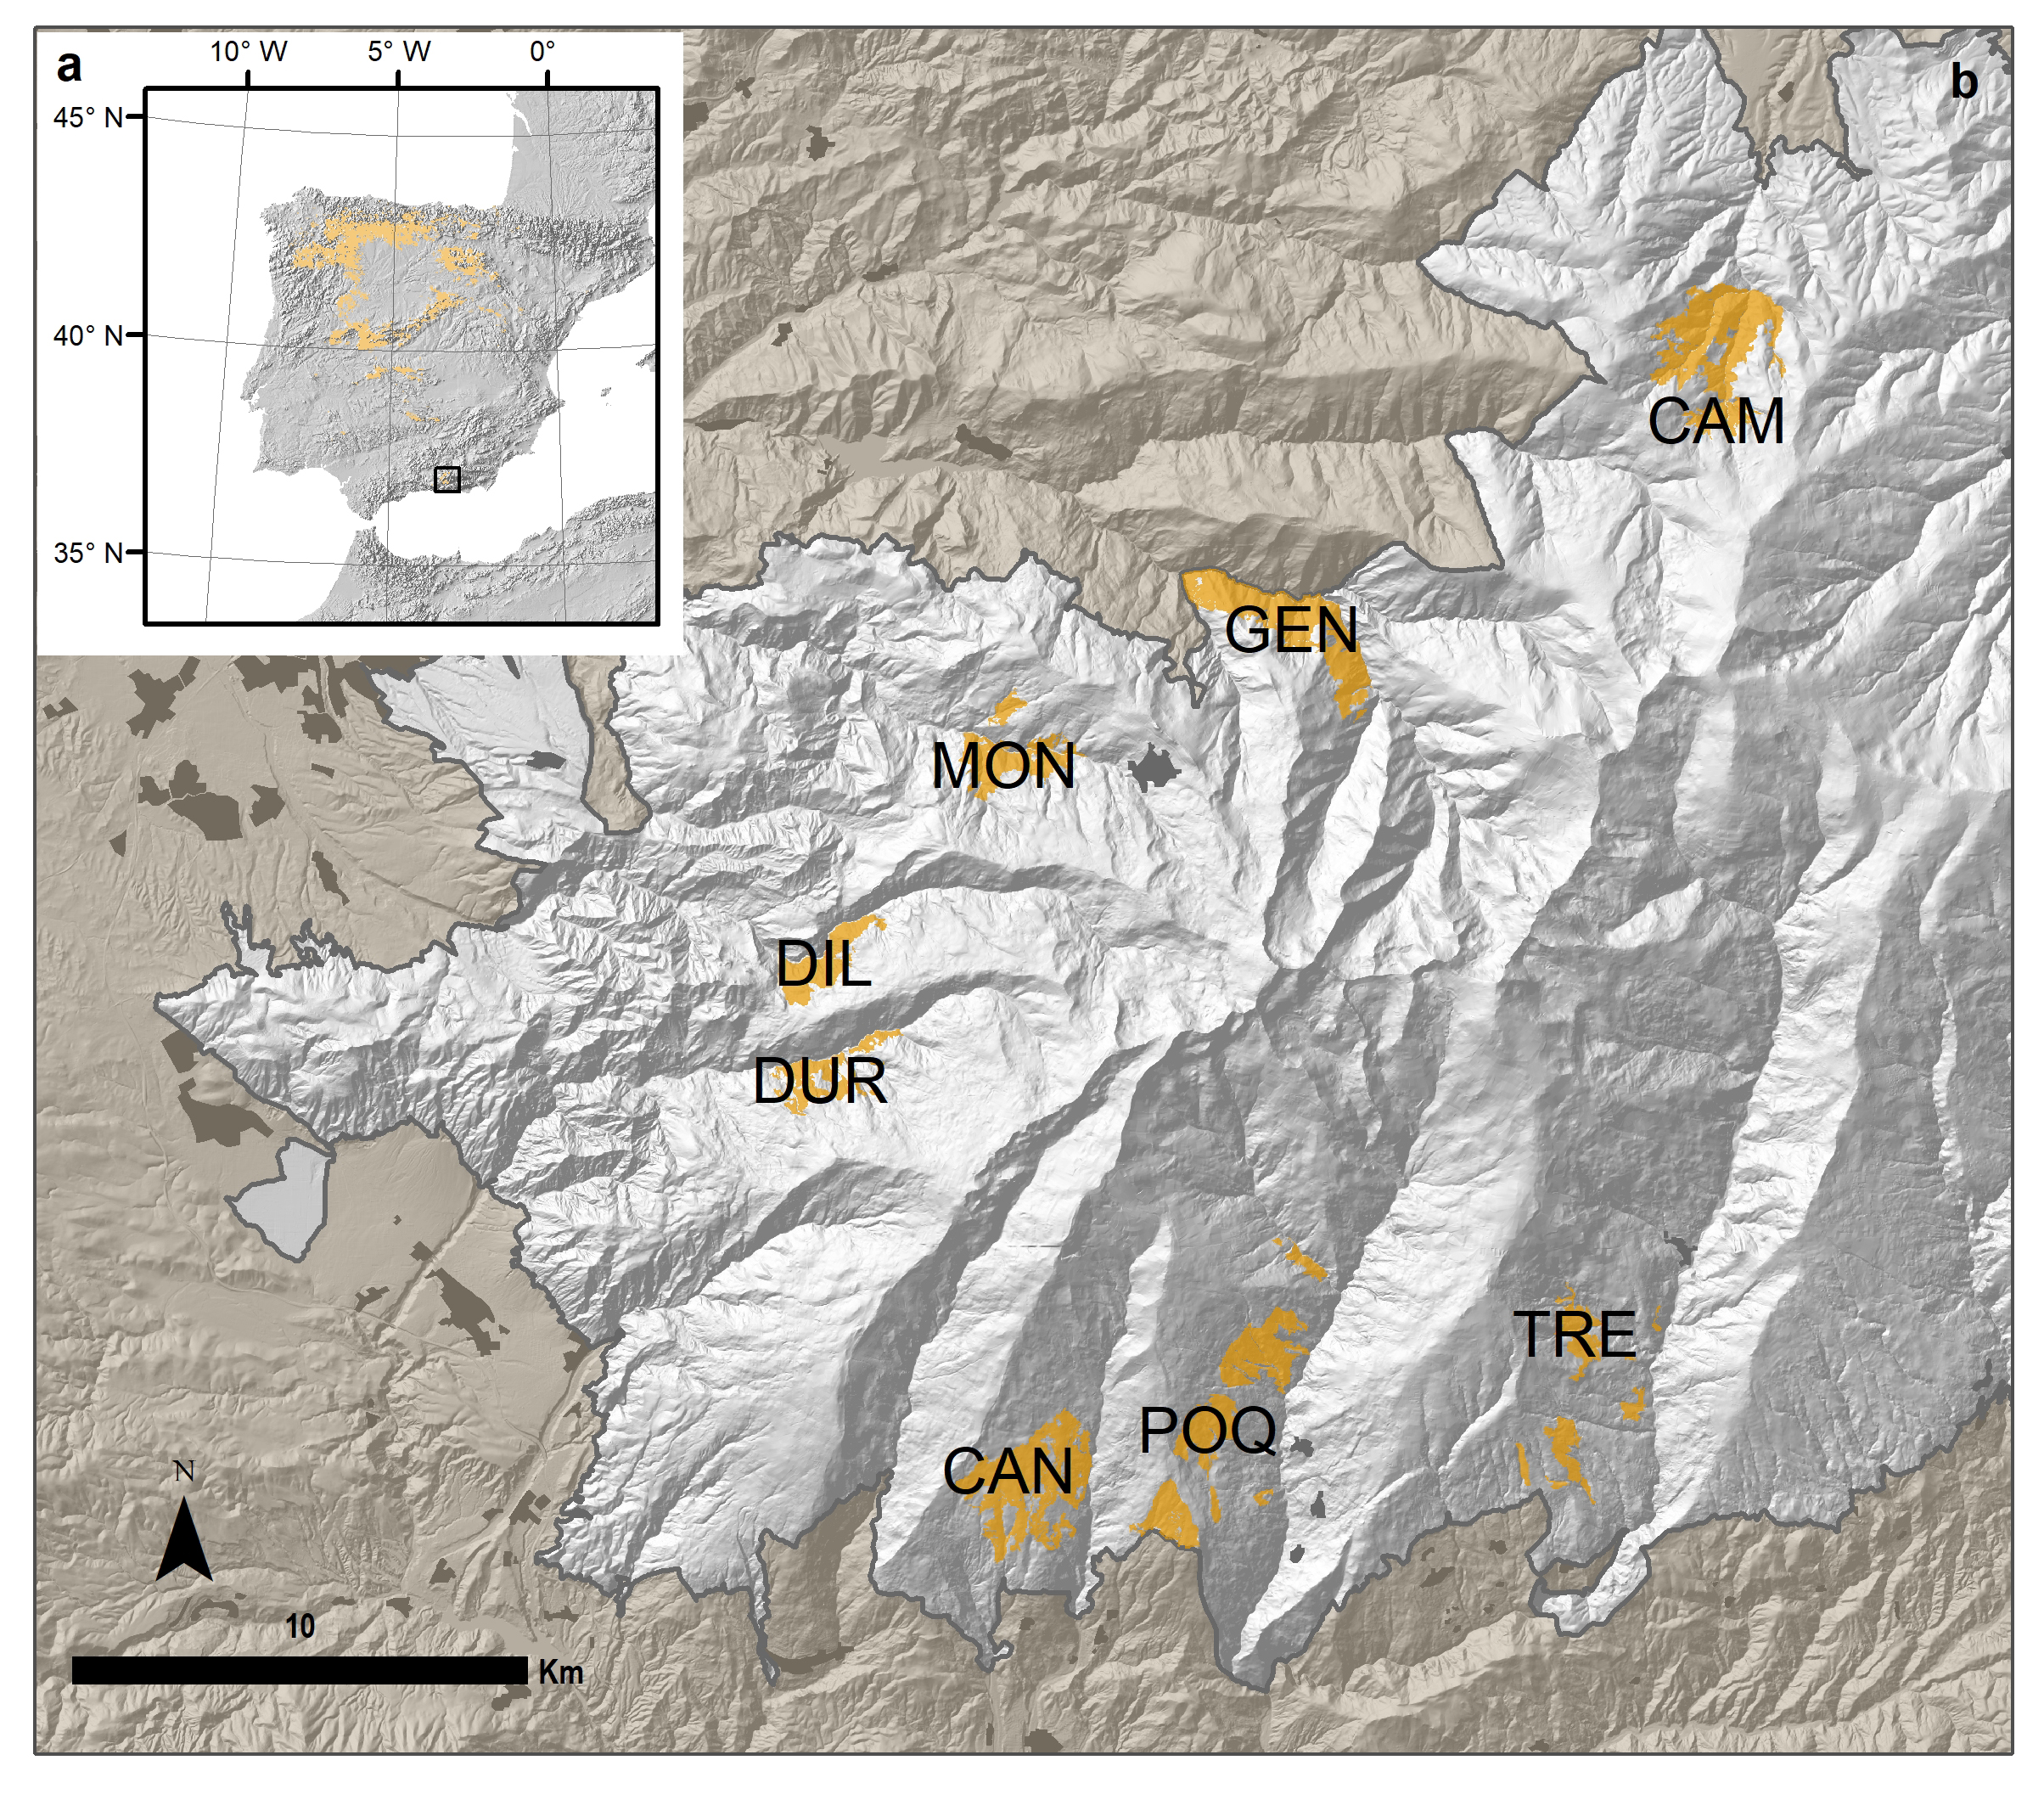
\includegraphics[width=0.7\textwidth]{img/multivariante/dist_map_multivariante} \caption{Distribution of \textit{Quercus pyrenaica} forests in the Iberian Peninsula (\textbf{a}) and location of the patches in Sierra Nevada mountain range (\textbf{b}). Name of the each population as in \tabref{tab:multivar:tpop}.}\label{fig:multivar:location-map}
\end{figure}

\section{Material and Methods}\label{sec:multivar:MatMet}
\subsection{Study area}\label{sec:multivar:StudyArea}
The study was conducted at the Sierra Nevada (Andalusia, SE Spain; \figref{fig:multivar:location-map}), a mountainous region covering more than 2000 km\textsuperscript{2} with an elevation range of between 860 and 3482 \emph{m.a.s.l.} The climate is Mediterranean, characterized by cold winters and hot summers, with a pronounced summer drought. The annual average temperature decreases in altitude from 12-16 ºC below 1500 \emph{m.a.s.l.} to 0 ºC above 3000 \emph{m.a.s.l.}. Annual precipitation ranges from less than 250 mm in the lowest areas of the mountain range to more than 700 mm in the highest peaks. Winter precipitation is mainly in the form of snow above 2000 \emph{m.a.s.l.}. Additionally, the complex orography causes strong climatic contrasts between south and north-facing slopes. This mountain range is considered one of the most important biodiversity hotspots in the Mediterranean region \autocite{Blancaetal1998ThreatenedVascular}, hosting 105 endemic plant species for a total of 2353 taxa of vascular plants (33\% and 20\% of Spanish and European flora, respectively) \autocite{Lorite2016UpdatedChecklist}. Forest cover in Sierra Nevada is dominated by pine plantations (\emph{Pinus halepensis} Mill., \emph{Pinus pinaster} Ait., \emph{Pinus nigra} Arnold subsp. \emph{salzmannii} (Dunal) Franco, and \emph{Pinus sylvestris} L.) covering approximately 37000 ha. Native forests are mainly dominated by holm oak (\emph{Quercus ilex} subsp. \emph{ballota} (Desf.) Samp.) occupying low and medium mountain areas (11000 ha.), and Pyrenean oak \Qpy ranging from 1100 to 2000 \emph{m.a.s.l.}, covering about 3000 ha \autocite{PerezLuqueetal2019MapEcosystems}.

\begin{sidewaystable} 
\caption{Description of the \Qp populations in Sierra Nevada. For elevation, minimum and maximum values are in brackets. The latitude and longitude coordinates referred to polygon centroid.}\label{tab:multivar:tpop}
\begin{adjustbox}{width=\linewidth}
	\begin{threeparttable}
		\begin{tabular}{@{}llllllll@{}}
			\toprule
			Oak poulation & Code & River valley & Municipalities & Elevation (m) & Latitude & Longitude & Area (ha) \\ \midrule
			El Camarate & CAM & Alhama & Lugros & 1740  (1441-2026) & 37º 10' 29.49'' N & 3º 15' 24.33'' W & 457.15 \\
			Robledal de San Juan & GEN & Genil & Güejar-Sierra & 1519  (1189-1899) & 37º 7' 29.63'' N & 3º 21' 54.60'' W & 395 \\
			Loma de la Perdíz & MON & Monachil & Monachil & 1780  (1564-1990) & 37º 5' 54.87'' N & 3º 25' 46.65'' W & 204.55 \\
			Umbría de la Dehesa de Dílar & DIL & Dílar & Dílar & 1764  (1478-1960) & 37º 3' 33.61'' N & 3º 28' 29.07'' W & 154.07 \\
			Loma de Enmedio & DUR & Dúrcal & Dúrcal & 1824  (1530-2035) & 37º 1' 58.75'' N & 3º 28' 38.44'' W & 137.04 \\
			El Robledal de Cáñar & CAN & Chico & Cáñar & 1687  (1366-1935) & 36º 57' 28.04'' N & 3º 25' 57.10'' W & 436.2 \\
			Loma de la Matanza y Loma de Ramón & POQ & Poqueira & Soportújar, Pampaneira, Bubión, Capileira & 1740  (1214-1981) & 36º 57' 58.90'' N & 3º 22' 55.12'' W & 458.95 \\
			Loma de los Lotes & TRE & Trevélez & Pórtugos, Busquístar & 1692  (1312-1963) & 36º 58' 37.38'' N & 3º 17' 25.75'' W & 197.92 \\ \bottomrule
		\end{tabular}
	\end{threeparttable}
\end{adjustbox}
\end{sidewaystable}

\Qpy is a deciduous species extending through southwestern France, the Iberian Peninsula and northern Morocco \autocite{Franco1990Quercus}. The forests of this species reach their southernmost European limit in Andalusian mountains such as Sierra Nevada, where eight populations have been identified (\figref{fig:multivar:location-map}a; \tabref{tab:multivar:tpop}) on the basis of their isolated geographic locations in deep valleys separated by distances considerably longer than the average dispersal distances of the seeds by birds such as Eurasian jay (\emph{Garrulus glandarius}) \autocite{Gomez2003SpatialPatterns,ValbuenaCarabanaetal2005GeneFlow}. They are distributed on siliceous soils both in the northwestern and southern slopes of the mountain range and are often associated to major river valleys. These oak woodlands represent a rear edge of their distribution \autocite{HampePetit2005ConservingBiodiversity}, containing high levels of intraspecific genetic diversity \autocite{ValbuenaCarabanaGil2013GeneticResilience}. Their conservation status for southern Spain is ``Vulnerable'', and it is expected to suffer from climate change, potentially reducing its suitable habitats in the near future \autocite{GeaIzquierdoetal2013GrowthProjections,GeaIzquierdoetal2017RiskyFuture}.

The distribution of \Qp forests in Sierra Nevada was delimited using the updated version of the forest map of Sierra Nevada at 1:10 000 scale \autocite{CMAOT2014CartografiaEvaluacion,PerezLuqueetal2019MapEcosystems}. Black and white ortophotographies from 2001 (0.5-m of spatial resolution) and false color aerial photographies (Color Infrared) from 2005 (1-m resolution) were used to correct errors by detailed photographic interpretation, resulting in a detailed map of oak forests (\figref{fig:multivar:location-map}b). Forest patches with at least 50 \% tree cover of which 75 \% cover being \Qp were considered oak patches.

\subsection{Environmental data}\label{sec:multivar:EnvData}
For each oak population we obtained the values of 30 environmental variables selected to represent different direct and indirect gradients important for plant distribution \autocite{GuisanZimmermann2000PredictiveHabitat,Williamsetal2012WhichEnvironmental}: temperature, water availability, topography, solar radiation and land-use (\tabref{tab:multivar:tvars}). Observed climate data (1960-2010) from 43 meteorological stations 50 km around Sierra Nevada, compiled by Sierra Nevada Global Change Observatory \autocite{Zamoraetal2017GlobalChange}, were used as input to compute high resolution (100 x 100 m pixel-size) climate maps \autocite{Benitoetal2014ClimateSimulations} based on the mapping method proposed by \textcite{Ninyerolaetal2000MethodologicalApproach}. Seasonal and annual maps with the averages of direct solar radiation and insolation time were computing using the GIS GRASS module r.sun \autocite{Neteleretal2012GRASSGIS,SuriHofierka2004NewGISbased}. From a high-resolution digital elevation model (10-m; Department of the Environment, Regional Government of Andalusia) several topographic variables were derived: elevation, slope, aspect, E-W and N-S gradients, topographic position (difference in elevation between a cell and surrounding cells within a 1000 meter radius)\autocite{Guisanetal1999GLMCCA}. Also, topographic wetness index and flow accumulation were computed using the r.terraflow module of GRASS GIS. As a surrogate of anthropogenic influence, we computed the frequency of human infrastructures in a 2000 meter radius buffer. Finally, for each environmental variable we extracted the values for all the 100 m size pixels contained within each oak population (\figref{fig:multivar:schemamulti}).

\newcommand{\Whm}{\(\mathrm{W \cdot h \cdot m^{-2}}\)}

\begin{table}[]
\caption{Description of environmental variables and forest attributes used in our analysis}\label{tab:multivar:tvars}
\centering
\begingroup\fontsize{7}{9}\selectfont
\begin{tabular}{llll} 
\toprule
\textbf{Category} & \textbf{Code} & \textbf{Description} & \textbf{Units} \\ 
\midrule
\multirow{13}{*}{Climate} & precYE & Annual precipitation & mm \\
 & precSU & Summer precipitation & mm \\
 & precAU & Autumn precipitation & mm \\
 & precWI & Winter precipitation & mm \\
 & precSP & Spring precipitation & mm \\
 & tmaxSU & Summer mean maximum temperature & º C \\
 & tmaxAU & Autumn mean maximum temperature & º C \\
 & tmaxWI & Winter mean maximum temperature & º C \\
 & tmaxSP & Spring mean maximum temperature & º C \\
 & tminSU & Summer mean minimum temperature & º C \\
 & tminAU & Autumn mean minimum temperature & º C \\
 & tminWI & Winter mean minimum temperature & º C \\
 & tminSP & Spring mean minimum temperature & º C \\ 
\hline
\multirow{16}{*}{Topography} & elev & Elevation & meter \\
 & aspect & Aspect & º \\
 & slope & Slope & º \\
 & tpNS & North-South gradient & \% \\
 & tpEW & East-West gradient & \% \\ 
 & radSU & Summer direct radiation & \Whm \\
 & radAU & Autumn direct radiation & \Whm \\
 & radWI & Winter direct radiation & \Whm \\
 & radSP & Spring direct radiation & \Whm \\
 & radhSU & Mean duration of insolation in Summer & hour \\
 & radhAU & Mean duration of insolation in Autumn & hour \\
 & radhWI & Mean duration of insolation in Winter & hour \\
 & radhSP & Mean duration of insolation in Spring & hour \\
 & twi & Topographic wetness index &  \\
 & tpos & Topographic position & meter \\
 & flow & Flow accumulation &  \\ 
\hline
Landscape & human & Anthropogenic influence & cells \\ 
\hline
\multirow{9}{*}{Forest structure} & FCC & Forest canopy cover & \% \\
 & FCCTree & Forest canopy cover of Tree & \% \\
 & FCCShru & Forest canopy cover of Shrub & \% \\
 & FCCHerb & Forest canopy cover of Herbaceous & \% \\
 & CCshann & Canopy Cover diversity &  \\
 & heiTree & Tree Height & m \\
 & denTree & Density & trees $ha^{-1}$ \\
 & BA & Basal area & $\mathrm{m^2 \cdot h^{-1}}$ \\
 & vol & Volume & $\mathrm{m^3 \cdot h^{-1}}$\\ 
\hline
\multirow{2}{*}{Forest biodiversity} & diver & Plant diversity &  \\
 & rich & Richness & species number \\ 
\hline
\multirow{3}{*}{Forest function} & regTot & Total regeneration & total seedling number \\
 & regQp & Pyrenean Oak regeneration & seedling number \\
 & regQi & Holm Oak regeneration & seedling number \\
\hline
\end{tabular}
\endgroup{}
\end{table}

\subsection{Forest attributes}\label{sec:multivar:ForAtri}
To characterize oak patches, we selected several stand attributes relating to forest structure, function, and composition from Sierra Nevada Forest Inventory \autocite[SINFONEVADA,][]{PerezLuqueetal2014SinfonevadaDataset} (\tabref{tab:multivar:tvars}). By using this approach, we characterized the plant community both in terms of their species composition, and also regarding their ecological functioning \autocite{McElhinnyetal2005ForestWoodland,delRioetal2016CharacterizationStructure}. SINFONEVADA forest inventory was carried out during 2004-2005, and it includes an extensive network of plots distributed within the main forest units of Sierra Nevada mountain range. We selected 32 plots belonging to deciduous broadleaf forests category. All of them are located within the eight Pyrenean oak populations identified in Sierra Nevada. For each plot (20 x 20 m), all trees with diameter at breast height (dbh) \textgreater{} 7.5 cm were tallied by species and dbh. Regeneration, species composition and abundance were also recorded in two additional subplots \autocite[see][ for a detailed description]{PerezLuqueetal2014SinfonevadaDataset}: a 5-m radius subplot where the seedling abundance of \Qp was recorded; and a 10-m radius subplot where the species composition and abundance estimated by the Braun-Blanquet cover-abundance scale were measured \autocite{BraunBlanquet1964PflanzensoziologieGrundzuge} (See \tabref{tab:multivar-s1}).

Forest composition (richness) and plant diversity were used as indicator for overall forest biodiversity. Plant diversity was measured using the Shannon diversity index \autocite{Krebs1999EcologicalMethodology}. The total regeneration was used as proxy for forest functioning. Finally, as forest structure indicators we selected the following attributes: the total- and strata- (\emph{i.e.} tree, shrub and herbaceous) canopy cover; canopy cover diversity; tree height, tree density, basal area and volume of adult tree. Canopy covers were computed as the proportion of plot area covered by the whole forest (total) and the different strata considered (tree, shrub and herbaceous respectively). Canopy cover diversity was quantified through the Shannon index for the proportion of plot area covered by different vegetation strata (tree, shrub and herbaceous) according with the following equation: \[CCd'=\sum_{i=1}^{n} g_i \cdot \ln g_i\] where \(g_i\) is the proportion of strata \(i\) of the total plot area and \(n\) is the number of strata \autocite{delRioetal2003IndicesStand}. Basal area was calculated as the sum of the basal areas of the adult trees assuming a circular cross-section of the trunk. Volume was calculated as sum of volume (\(V = 0.55 \cdot \textrm{height} \cdot \textrm{diameter}^2\)) of all \Qp adult trees. Additionally, we also extracted the values of the environmental variables for the centroids of the plots and we added a species-composition matrix for each of the 32 selected plots.

\begin{figure}
\centering
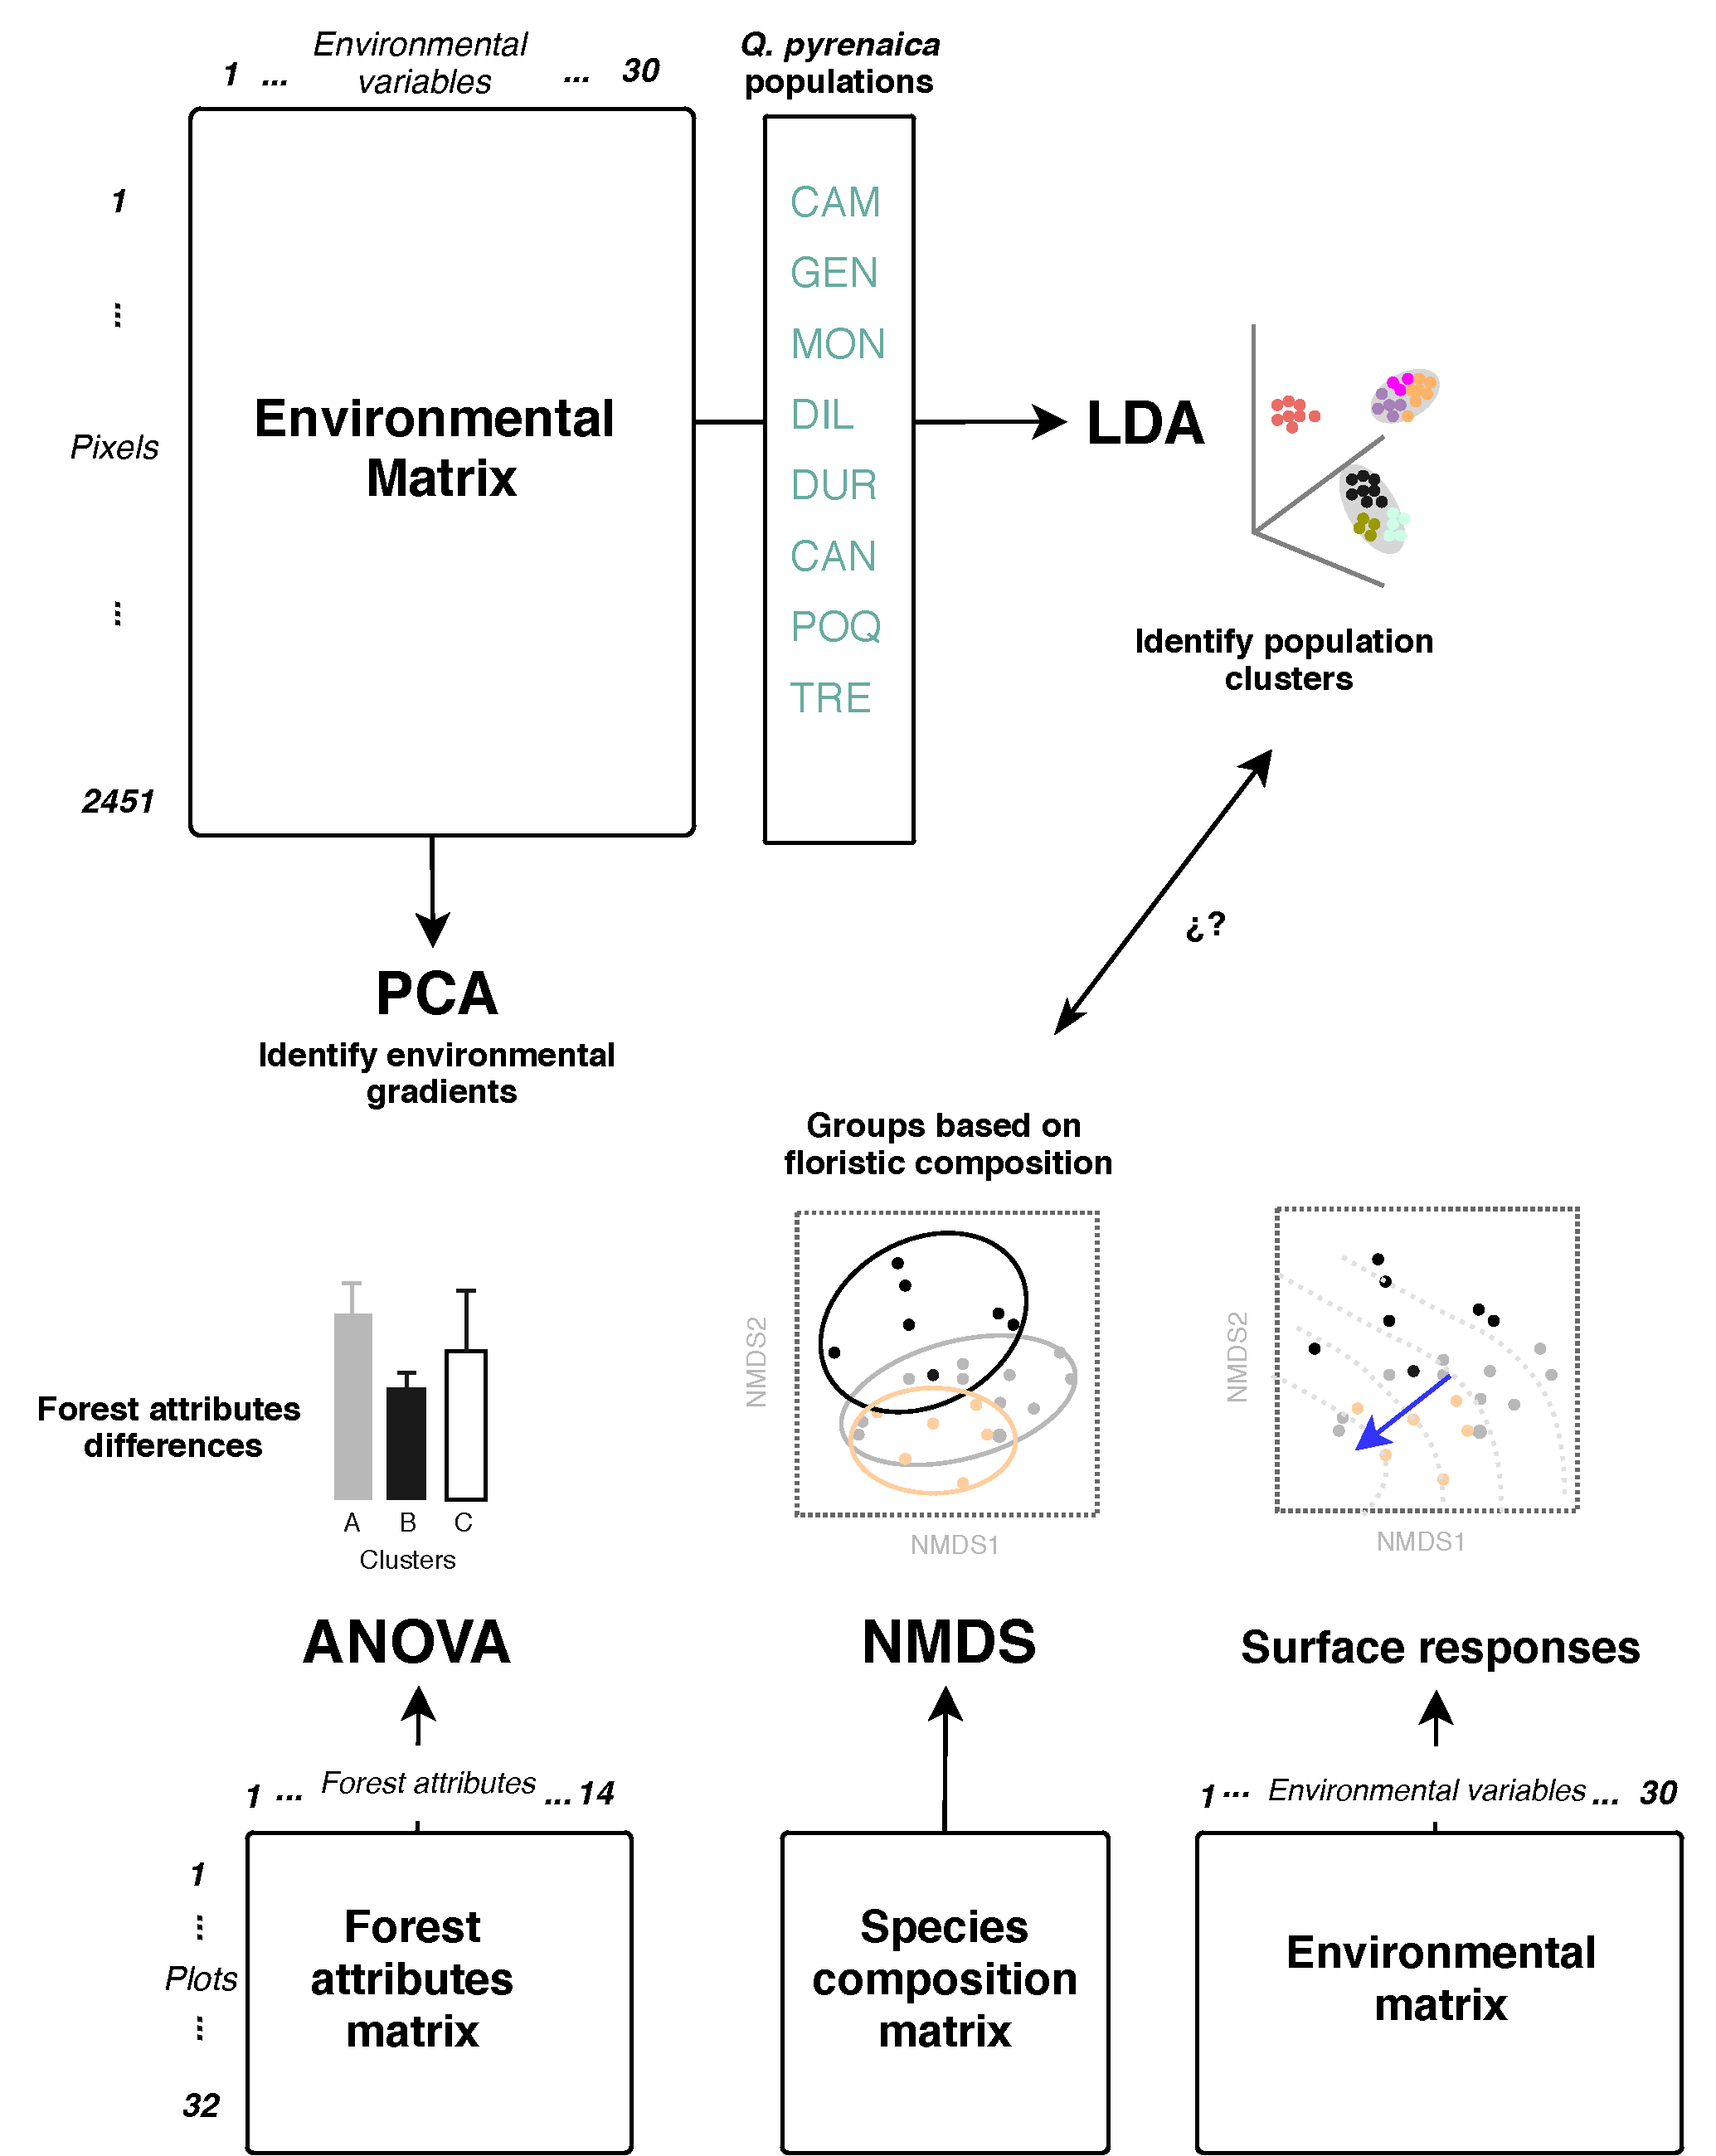
\includegraphics[height= 13cm]{img/multivariante/schema} \caption{Methodological scheme of the analyses. Using an environmental data matrix, the main environmental gradients that characterize the oak forests at Sierra Nevada were identified using a Principal Component Analysis (PCA). Linear Discriminant Analysis (LDA) was also applied to identify different groups of oak populations. With a matrix of floristic composition, a Non-metric Multidimensional Scaling (NMDS) ordination were applied to visualize patterns of species composition, interpret them according to the environmental factors, and identify groups of oak populations based on similarities between floristic composition. See material and methods for more details.} \label{fig:multivar:schemamulti}
\end{figure}

\subsection{Statistical analysis}\label{sec:multivar:Analysis}
To identify the main environmental gradients that characterize the oak forests at Sierra Nevada, we performed a principal component analysis (PCA) on the standardized variables (\figref{fig:multivar:schemamulti}). Over 75 \% of the correlations (Sperman's r) among variables were significant (p \textless{} 0.01). We checked the adequacy of the environmental matrix by applying Kaiser-Meyer-Olkin test, a measure of sampling adequacy (KMO=0.7138, value greater than 0.5 is considered adequate \autocite{DziubanShirkey1974WhenCorrelation}. The Kaiser-Guttman rule {[}\emph{i.e.} axes whose eigenvalues are larger than the average of all eigenvalues; \textcite{Guttman1954NecessaryConditions}{]}, and the criterion that any principal component (PC) accounts for at least 10\% of the total variance were used to determine the meaningful PCs to be retained for interpretation \autocite{LegendreLegendre2012NumericalEcology}. The PCA variables with a correlation to the principal components that was higher than 0.7 were selected to describe the environmental gradients indicated by the principal factors. We applied Linear Discriminant analysis (LDA) to determine the environmental variables that best discriminated among Pyrenean oak patches and to identify different groups of populations \autocite{Williams1983ObservationsUse,LegendreLegendre2012NumericalEcology}.

Then, environmental variables and forest attributes were tested for differences among populations groups previously identified. Normality and homoscedasticity were checked using the Shapiro-Wilk test and Levene's test respectively. If normality and homoscedasticity assumptions were satisfied, we performed ANOVA analysis followed by the Tukey LSD for testing statistical significance. Otherwise, Kruskal-Wallis ANOVA for nonparametric data were conducted followed by manual pairwise comparison using Mann-Whitney U-test.

Finally we used a Non-metric Multidimensional Scaling (NMDS) ordination analysis based on Bray--Curtis dissimilarity distance \autocite{Kruskal1964NonmetricMultidimensional} to: (\emph{i}) visualize patterns of species compositions, (\emph{ii}) interpret them with respect to the environmental factors (\emph{i.e.} relate the variability in species composition to environmental variables), and (\emph{iii}) identify groups of Pyrenean oak populations based on similarities between floristic composition. NMDS involves the reduction of multidimensional similarity data to a low-dimensional ordination in which relative distance indicates relative similarity (\emph{i.e.} plots with very similar species composition are close and \emph{vice versa}) \autocite{Minchin1987SimulationMultidimensional}. We compared two and three-dimensional solutions based on Kruskal's stress (as a measure of goodness of fit). We also studied the floristic-environment relationships by fitting linear trends on the ordination yielded by the NMDS. For these linear fittings, squared correlation coefficients and empirical p-values were calculated using random permutations (n = 1000) of the data \autocite{Oksanen2013MultivariateAnalysis}. Finally we fitted non-parametrically smoothed surfaces of continuous environmental variables on the NMDS ordination. The smooth surfaces were fitted using generalized additive models (GAM) with thin plate splines, using the coefficient of determination (\(R^2\)) as goodness-of-fit statistic \autocites[\emph{e.g.}][]{Oksanen2013MultivariateAnalysis,Virtanenetal2006BroadScale}.

All analysis was conducted in R software \autocite{RCoreTeam2019LanguageEnvironment} using the following packages: MASS \autocite{MASS}, nFactors \autocite{nFactors}, and vegan \autocite{vegan}. We also used the packages candisc \autocite{candisc}, ellipse \autocite{ellipse}, ggpubr \autocite{ggpubr}, ggord \autocite{ggord}, factoextra \autocite{factoextra} and patchwork \autocite{patchwork} for visualization.

\section{Results}\label{sec:multivar:Results}
PCA of all measured environmental variables yielded three significant axes explained 62.11 \% of the total variance (\tabref{tab:multivar:tpca}). The first PC axis was strong and negatively correlated with radiation and precipitation related variables, and positively with northness gradient and slope (\tabref{tab:multivar:tpca}). Maximum average temperatures showed strongest negative correlations with the second PC axis. The third PC axis was negatively correlated with minimum average temperatures. The precipitation variables presented weak positive correlation with the third PC axis.

\begin{table}
\caption{Results of the principal component and discriminant analysis. The three first axis for PCA and LDA are shown. Loadings and correlations of the environmental variables on principal component axis are reported. For LDA, canonical correlations of environmental variables with each discriminant function are shown.}
\begin{table}[H]
\centering
\resizebox{\linewidth}{!}{
\begin{tabular}{lrrrrrrrrr}
\toprule
\textbf{Variable} & \textbf{PC1 load} & \textbf{PC1 cor.} & \textbf{PC2 load} & \textbf{PC2 cor.} & \textbf{PC3 load} & \textbf{PC3 cor.} & \textbf{LDA 1} & \textbf{LDA 2} & \textbf{LDA 3}\\
\midrule
\addlinespace[0.3em]
\multicolumn{10}{l}{\textbf{Topography}}\\
\hspace{1em}twi & -0.022 & -0.069 & -0.010 & -0.024 & 0.023 & 0.046 & -0.009 & 0.005 & 0.018\\
\hspace{1em}flow & 0.024 & 0.073 & 0.011 & 0.026 & -0.008 & -0.015 & 0.004 & -0.003 & 0.005\\
\hspace{1em}elev & -0.158 & -0.489 & -0.016 & -0.035 & 0.142 & 0.280 & 0.000 & -0.014 & 0.105\\
\hspace{1em}slope & 0.222 & 0.690 & -0.068 & -0.155 & 0.157 & 0.309 & 0.032 & 0.034 & -0.073\\
\hspace{1em}tpos & -0.163 & -0.507 & -0.019 & -0.042 & -0.043 & -0.085 & -0.021 & -0.013 & 0.006\\
\hspace{1em}aspect & -0.210 & -0.650 & -0.012 & -0.026 & -0.087 & -0.172 & -0.044 & -0.043 & 0.075\\
\hspace{1em}tpEW & 0.082 & 0.255 & 0.092 & 0.209 & -0.017 & -0.033 & 0.029 & 0.065 & 0.044\\
\hspace{1em}tpNS & 0.238 & 0.737 & 0.031 & 0.070 & 0.092 & 0.182 & 0.076 & 0.070 & -0.070\\
\hspace{1em}radWI & -0.270 & -0.836 & -0.030 & -0.067 & -0.101 & -0.198 & -0.071 & -0.076 & 0.081\\
\hspace{1em}radSU & -0.276 & -0.857 & -0.023 & -0.051 & -0.119 & -0.235 & -0.067 & -0.077 & 0.084\\
\hspace{1em}radSP & -0.287 & -0.889 & 0.031 & 0.071 & -0.152 & -0.299 & -0.045 & -0.059 & 0.090\\
\hspace{1em}radAU & -0.292 & -0.906 & 0.005 & 0.011 & -0.141 & -0.279 & -0.056 & -0.069 & 0.090\\
\hspace{1em}radhWI & -0.286 & -0.888 & -0.014 & -0.032 & -0.127 & -0.251 & -0.073 & -0.083 & 0.098\\
\hspace{1em}radhSP & -0.283 & -0.878 & 0.024 & 0.054 & -0.150 & -0.295 & -0.051 & -0.054 & 0.101\\
\hspace{1em}radhSU & -0.138 & -0.428 & 0.111 & 0.252 & -0.105 & -0.207 & -0.003 & 0.003 & 0.061\\
\hspace{1em}radhAU & -0.190 & -0.590 & 0.096 & 0.218 & -0.112 & -0.220 & -0.018 & -0.003 & 0.074\\
\addlinespace[0.3em]
\multicolumn{10}{l}{\textbf{Landscape}}\\
\hspace{1em}human & -0.143 & -0.443 & -0.069 & -0.156 & 0.165 & 0.326 & -0.067 & 0.013 & 0.107\\
\addlinespace[0.3em]
\multicolumn{10}{l}{\textbf{Climate}}\\
\hspace{1em}precWI & -0.191 & -0.593 & -0.178 & -0.404 & 0.301 & 0.594 & -0.081 & 0.024 & -0.076\\
\hspace{1em}precSP & -0.178 & -0.551 & -0.068 & -0.153 & 0.264 & 0.520 & -0.044 & 0.087 & 0.074\\
\hspace{1em}precSU & -0.226 & -0.702 & -0.084 & -0.190 & 0.243 & 0.479 & -0.073 & 0.069 & 0.092\\
\hspace{1em}precAU & -0.223 & -0.692 & -0.173 & -0.391 & 0.225 & 0.444 & -0.157 & -0.043 & -0.074\\
\hspace{1em}precYE & -0.223 & -0.692 & -0.145 & -0.329 & 0.274 & 0.539 & -0.092 & 0.032 & -0.001\\
\hspace{1em}tminWI & 0.042 & 0.131 & -0.342 & -0.775 & -0.267 & -0.525 & 0.003 & -0.001 & -0.024\\
\hspace{1em}tminSP & 0.036 & 0.110 & -0.293 & -0.664 & -0.311 & -0.613 & 0.007 & -0.008 & 0.001\\
\hspace{1em}tminSU & 0.022 & 0.068 & -0.189 & -0.429 & -0.357 & -0.705 & 0.014 & -0.011 & 0.045\\
\hspace{1em}tminAU & 0.035 & 0.109 & -0.276 & -0.625 & -0.321 & -0.633 & 0.009 & -0.009 & 0.008\\
\hspace{1em}tmaxWI & 0.051 & 0.159 & -0.353 & -0.800 & 0.133 & 0.262 & -0.021 & 0.014 & -0.176\\
\hspace{1em}tmaxSP & 0.063 & 0.196 & -0.355 & -0.804 & 0.091 & 0.180 & -0.009 & -0.014 & -0.155\\
\hspace{1em}tmaxSU & 0.056 & 0.175 & -0.396 & -0.897 & 0.015 & 0.030 & -0.010 & 0.004 & -0.120\\
\hspace{1em}tmaxAU & 0.054 & 0.166 & -0.372 & -0.843 & 0.100 & 0.196 & -0.018 & 0.011 & -0.160\\
\addlinespace[0.3em]
\multicolumn{10}{l}{\textbf{}}\\
\hspace{1em}Eigenvalue & 9.618 &  & 5.130 &  & 3.886 &  & 150.351 & 67.162 & 19.108\\
\hspace{1em}Variance & 32.061 &  & 17.100 &  & 12.953 &  & 61.780 & 27.597 & 7.851\\
\hspace{1em}Cumulated variance & 32.061 &  & 49.161 &  & 62.114 &  & 61.780 & 89.378 & 97.229\\
\hspace{1em}Canonical correlation &  &  &  &  &  &  & 0.997 & 0.993 & 0.975\\
\bottomrule
\end{tabular}}
\end{table}
\label{tab:multivar:tpca}
\end{table}

\begin{figure}
\centering
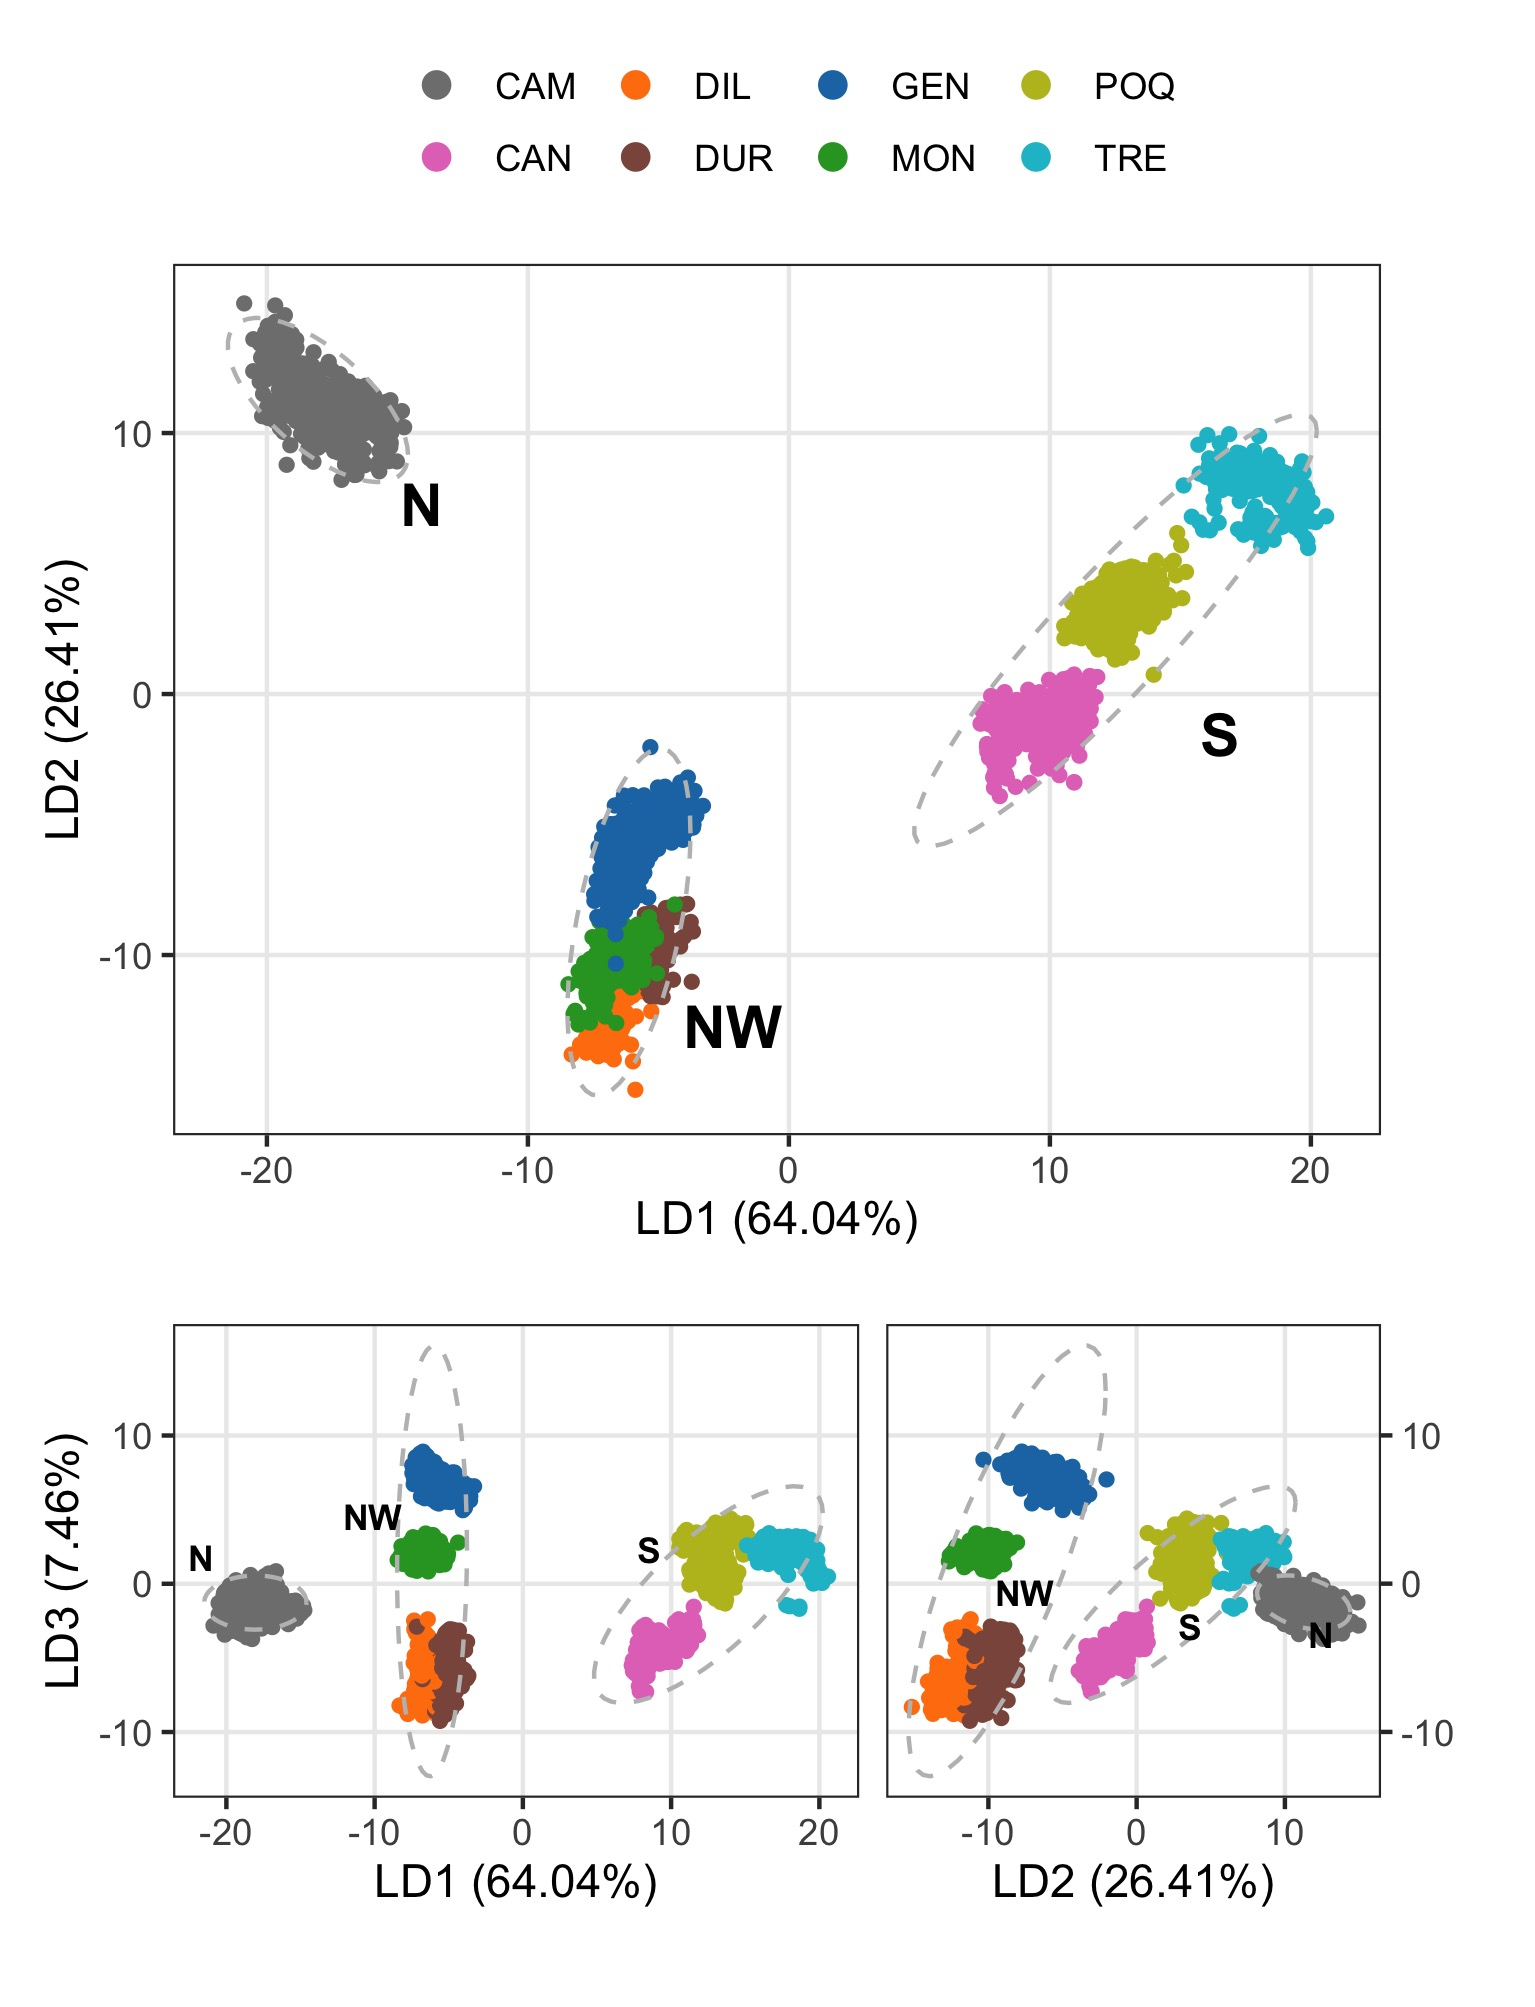
\includegraphics[width=0.7\textwidth]{img/multivariante/lda_biplotsv2} \caption{Discriminant analysis ordination of \textit{Quercus pyrenaica} populations. N: northern population group (CAM); NW: northwest population group (GEN, MON, DUR, DIL); and S: southern population group (CAN, POQ, TRE). Population's code as in  \tabref{tab:multivar:tpop}. Numbers in brackets expressed explained variance (\%) for each discriminant axis.} \label{fig:multivar:lda}
\end{figure}

The discriminant analysis yielded three significant functions explaining 97.9 \% of variance (\tabref{tab:multivar:tpca}). The ordination plot (\figref{fig:multivar:lda}) showed a clear separation of oak populations into three clusters: a single-oak-population (CAM) cluster, namely N in the \figref{fig:multivar:lda}; the second cluster (NW) formed by the GEN, MON, DIL and DUR oak populations; and the southern cluster (S) composed by the southern oak populations CAN, POQ and TRE. Southern oak populations were separated out from northern populations along the first LDA axis (\figref{fig:multivar:lda}), which showed slight negatively correlation with autumn rainfall. The second and third LDA axes showed weak correlations with all variables (\tabref{tab:multivar:tpca}).

The three oak clusters showed significantly differences for most of the environmental variables analyzed (\tabref{tab:multivar:tanovas}). Only winter minimum temperatures (\(\chi^2\) = 5.35; p-value = 0.069) and insolation time during summer (\(\chi^2\) = 0.306; p-value = 0.306)) was similar among the three oak clusters (\tabref{tab:multivar:tanovas}). \emph{Post-hoc} analysis showed that for most of the environmental variables we found pairwise significant differences between all the three oak clusters (\tabref{tab:multivar:tanovas}).

Forest attributes did not significantly differ among the above described oak clusters except for plant diversity and herbaceous canopy cover (\tabref{tab:multivar:tanovas}). The N cluster showed higher value of Shannon diversity index (2.27 ± 0.17) than NW cluster (\emph{Mann-Whitney U} = 22.0; p-value \textless0.01). For stand attributes relating to forest structure only the herbaceous canopy cover showed significantly differences (\(\chi^2\) = 11.18; p-value = 0.004; \tabref{tab:multivar:tanovas}) between N and NW clusters (\emph{Mann-Whitney U} = 15.0; p-value \textless{} 0.01). For all other forest structure attributes, despite there are no significant differences, the N cluster showed the lowest values (\tabref{tab:multivar:tanovas}). No significant differences were recorded for regeneration variables.

\begin{table}
\caption{Mean values of environmental variables and forest attributes for the three identified clusters of \textit{Q. pyrenaica} forests derivated from the discriminant anaylisis. The Chi-squared statistics of the nonparametric Kruskal-Wallis test is shown except for those variables analyzed using ANOVA test (\textit{fccShru}, \textit{fccTree} and \textit{rich}). Values within brackets correspond to standard errors. Standard erros are shown in parentheses. Different letters indicate statistically significant differences between clusters oak populations.}\label{tab:multivar:tanovas}
\centering\begingroup\fontsize{7}{9}\selectfont
\begin{tabular}{lrrllll}
\toprule
\textbf{variable} & \textbf{statistic} & \textbf{p.value} & \textbf{d.f.} & \textbf{groupA (N)} & \textbf{groupB (NW)} & \textbf{groupC (S)}\\
\midrule
\addlinespace[0.3em]
\multicolumn{7}{l}{\textbf{Forest attributes}}\\
\hspace{1em}BA & 4.43 & 0.109 & 2 & 0.71 (0.47) a & 7.11 (2.00) ab & 7.71 (2.78) b\\
\hspace{1em}denTree & 3.17 & 0.204 & 2 & 61.57 (31.95) a & 226.97 (65.10) a & 282.47 (86.03) a\\
\hspace{1em}fccHerb & 11.18 & 0.004 & 2 & 6.50 (0.60) a & 2.83 (0.51) b & 4.33 (1.12) ab\\
\hspace{1em}fcc & 4.45 & 0.108 & 2 & 7.50 (0.57) a & 8.50 (0.54) a & 8.67 (0.99) a\\
\hspace{1em}heiTree & 1.15 & 0.563 & 2 & 4.19 (1.67) a & 6.96 (1.83) a & 7.45 (1.76) a\\
\hspace{1em}CCShann & 2.09 & 0.352 & 2 & 0.85 (0.06) a & 0.92 (0.04) a & 0.93 (0.04) a\\
\hspace{1em}vol & 3.63 & 0.163 & 2 & 7.50 (4.92) a & 90.05 (29.24) a & 76.66 (34.22) a\\
\hspace{1em}fccShru & 1.96 & 0.159 & 2,29 & 2.75 (0.86) a & 4.50 (0.51) a & 5.33 (1.54) a\\
\hspace{1em}fccTree & 1.41 & 0.261 & 2,29 & 1.75 (0.62) a & 3.33 (0.58) a & 2.67 (0.80) a\\
\hspace{1em}regTot & 0.18 & 0.913 & 2 & 19.38 (6.25) a & 47.56 (16.16) a & 32.67 (15.82) a\\
\hspace{1em}regQi & 3.89 & 0.143 & 2 & 5.75 (3.40) a & 0.17 (0.09) a & 3.50 (2.08) a\\
\hspace{1em}regQp & 0.39 & 0.823 & 2 & 7.62 (3.21) a & 46.39 (16.16) a & 29.17 (16.30) a\\
\hspace{1em}diver & 8.67 & 0.013 & 2 & 2.27 (0.17) a & 1.57 (0.13) b & 1.83 (0.09) ab\\
\hspace{1em}rich & 2.95 & 0.068 & 2,29 & 16.62 (1.95) a & 11.72 (1.21) a & 14.17 (0.70) a\\
\addlinespace[0.3em]
\multicolumn{7}{l}{\textbf{Environmental}}\\
\hspace{1em}flow & 66.22 & 0.000 & 2 & 345.35 (97.91) a & 175.73 (32.95) b & 169.57 (21.93) c\\
\hspace{1em}twi & 60.74 & 0.000 & 2 & 4.90 (0.08) a & 5.08 (0.05) b & 5.40 (0.05) c\\
\hspace{1em}elev & 32.38 & 0.000 & 2 & 1740.05 (6.52) a & 1669.84 (6.22) b & 1710.33 (4.20) c\\
\hspace{1em}tpEW & 442.28 & 0.000 & 2 & 40.37 (1.47) a & 54.36 (0.84) b & 28.34 (0.58) c\\
\hspace{1em}tpos & 201.90 & 0.000 & 2 & -22.52 (1.73) a & -22.46 (1.64) a & -1.25 (0.75) b\\
\hspace{1em}aspect & 656.80 & 0.000 & 2 & 160.25 (5.50) a & 113.33 (2.33) b & 262.06 (3.14) c\\
\hspace{1em}slope & 568.14 & 0.000 & 2 & 26.10 (0.33) a & 29.93 (0.28) b & 20.32 (0.25) c\\
\hspace{1em}radWI & 1301.22 & 0.000 & 2 & 1489.98 (50.78) a & 770.18 (31.99) b & 3013.85 (25.28) c\\
\hspace{1em}radAU & 1238.90 & 0.000 & 2 & 5854.49 (40.75) a & 5205.08 (30.85) b & 6808.90 (17.59) c\\
\hspace{1em}radSU & 1242.79 & 0.000 & 2 & 3056.60 (59.95) a & 2140.28 (41.68) b & 4619.39 (26.39) c\\
\hspace{1em}radSP & 1064.83 & 0.000 & 2 & 6835.85 (29.69) a & 6352.91 (25.49) b & 7419.43 (14.46) c\\
\hspace{1em}radhWI & 1565.28 & 0.000 & 2 & 4.77 (0.10) a & 2.98 (0.08) b & 8.10 (0.05) c\\
\hspace{1em}radhAU & 125.57 & 0.000 & 2 & 10.44 (0.05) a & 10.37 (0.04) a & 11.01 (0.03) b\\
\hspace{1em}radhSP & 1117.91 & 0.000 & 2 & 7.42 (0.06) a & 6.47 (0.06) b & 9.13 (0.04) c\\
\hspace{1em}radhSU & 2.36 & 0.307 & 2 & 11.49 (0.05) a & 11.37 (0.04) a & 11.58 (0.03) a\\
\hspace{1em}tpNS & 1363.86 & 0.000 & 2 & 62.33 (0.93) a & 73.73 (0.66) b & 27.76 (0.54) c\\
\hspace{1em}dist & 2094.16 & 0.000 & 2 & 47.10 (0.04) a & 39.52 (0.11) b & 25.26 (0.04) c\\
\hspace{1em}human & 983.67 & 0.000 & 2 & 0.00 (0.00) a & 6.95 (0.38) b & 19.53 (0.45) c\\
\hspace{1em}precYE & 1143.00 & 0.000 & 2 & 690.32 (1.66) a & 741.43 (1.10) b & 778.13 (0.95) c\\
\hspace{1em}precWI & 926.56 & 0.000 & 2 & 233.38 (0.43) a & 246.53 (0.27) b & 253.85 (0.28) c\\
\hspace{1em}precAU & 1703.96 & 0.000 & 2 & 253.82 (0.45) a & 267.02 (0.29) b & 290.49 (0.35) c\\
\hspace{1em}precSP & 576.54 & 0.000 & 2 & 135.36 (0.39) a & 148.30 (0.32) b & 148.28 (0.21) c\\
\hspace{1em}precSU & 847.35 & 0.000 & 2 & 67.76 (0.39) a & 79.57 (0.32) b & 85.51 (0.20) c\\
\hspace{1em}tmaxWI & 184.76 & 0.000 & 2 & 8.22 (0.05) a & 9.40 (0.05) b & 9.16 (0.04) c\\
\hspace{1em}tmaxAU & 170.76 & 0.000 & 2 & 16.22 (0.05) a & 17.19 (0.05) b & 16.97 (0.04) c\\
\hspace{1em}tmaxSP & 46.60 & 0.000 & 2 & 13.95 (0.04) a & 14.35 (0.04) b & 14.21 (0.03) c\\
\hspace{1em}tmaxSU & 87.50 & 0.000 & 2 & 24.93 (0.04) a & 25.46 (0.04) b & 25.29 (0.03) c\\
\hspace{1em}tminWI & 5.35 & 0.069 & 2 & 0.45 (0.04) a & 0.42 (0.02) a & 0.37 (0.02) a\\
\hspace{1em}tminAU & 28.56 & 0.000 & 2 & 7.15 (0.04) a & 6.93 (0.02) b & 6.89 (0.02) b\\
\hspace{1em}tminSP & 18.45 & 0.000 & 2 & 4.55 (0.04) a & 4.37 (0.02) b & 4.35 (0.02) b\\
\hspace{1em}tminSU & 80.11 & 0.000 & 2 & 13.13 (0.04) a & 12.68 (0.03) b & 12.68 (0.03) b\\
\bottomrule
\end{tabular}
\endgroup{}
\end{table}

A three-dimensional solution of the NMDS was chosen because its correlation with the original data was higher than for a two-dimensional solution (Linear fit \(R^2\)=0.793 \emph{vs.} 0.713). Additionally, lower Kruskal's stress value was observed for the three-dimensional solution (Stress=0.159 \emph{vs.} 0.226). The NMDS ordination of the forest stands according to their floristic composition was significantly correlated with precipitation variables, elevation and marginally with winter maximum temperatures (\figref{fig:multivar:nmds}; \tabref{tab:multivar:nmds}). The precipitation variables showed highly and negative correlations with NMDS axis 2 (\tabref{tab:multivar:nmds}). The NMDS axis 1 were negatively correlated with elevation (\(R^2\) = 0.464) and minimum temperatures, and positively correlated with slope and winter maximum temperatures (Table \ref{tab:multivar:nmds}). The NMDS ordinations with fitted vectors and surfaces for significant variables are shown in \figref{fig:multivar:surfaces}. All these variables showed a non-linear significant relationship with the ordination pattern (\(R^2\) values for surfaces were slightly higher than linear \(R^2\) values; \tabref{tab:multivar:nmds}).

\begin{figure}
\centering
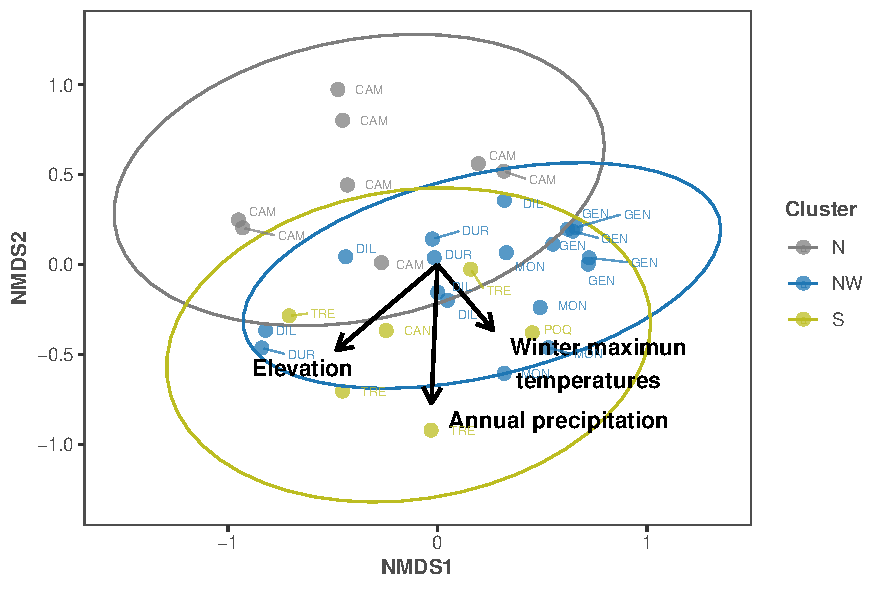
\includegraphics[width=0.8\textwidth]{img/multivariante/nmds} 
\caption{NMDS ordination of the plots. Points represent plot sites displayed according to their similarity in species composition. Proximity in the statistical space indicates plot sites with a similar species composition. Arrows represent vectors of significantly environmental variables explaining the ordination (see \tabref{tab:multivar:nmds}). Each plot coloured according to the three oak-populations clusters derived from discriminant analysis. Only two dimensions of the NMDS is illustrated for ease of representation.} 
\label{fig:multivar:nmds}
\end{figure}

\section{Discussion}\label{sec:multivar:Discussion}
\subsection{Ecological diversity within the rear-edge}\label{sec:multivar:EcolDiversity}

The rear-edge populations of \Qpy located in mountain areas are not ecologically homogeneous, neither for their environmental conditions nor for their plant species composition. In this study, we find separate groups of \Qp populations within Sierra Nevada (rear-edge) driven by radiation and rainfall as main discriminant variables (\figref{fig:multivar:lda}). The differences among populations based on environmental variables, are in line with differential ecological dynamics reported for \Qp forests in the Sierra Nevada by other studies. For instance, primary productivity of these forest measured using remote sensing showed a heterogeneous spatial behavior, with oak woodlands of the southern slopes displaying a greater annual vegetation greenness than those from the northern slopes \autocite{Dionisioetal2012SatelliteBasedMonitoring,PerezLuqueetal2015OntologicalSystem,PerezLuqueetal2020LanduseLegacies}. Also, differences have been found in both seasonal dynamics of greenness \autocite{Dionisioetal2012SatelliteBasedMonitoring}, and in temporal trends for primary productivity in the last years related with differential snow-cover trends in contrasting slopes \autocite{PerezLuqueetal2015OntologicalSystem,AlcarazSeguraetal2016ChangesVegetation}.

\begin{figure}
\centering
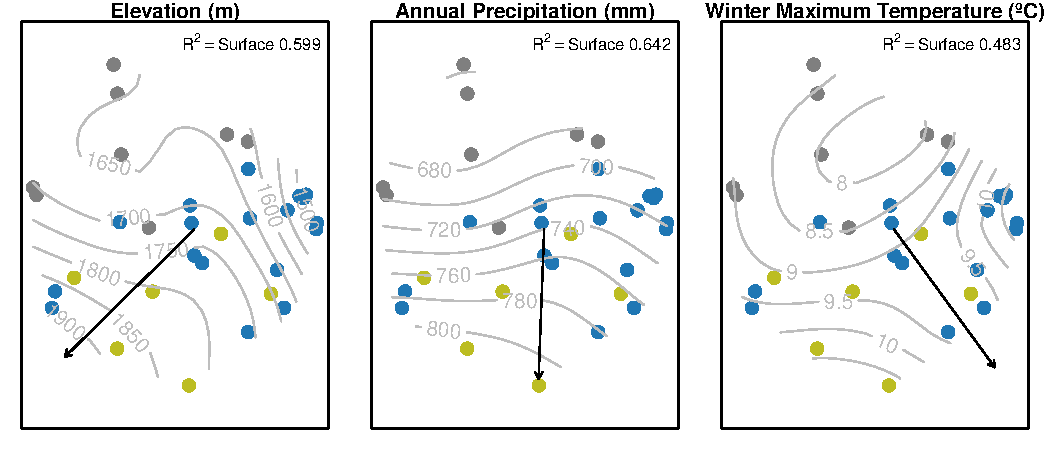
\includegraphics[width=\textwidth]{img/multivariante/surfaces} 
\caption{NMDS ordination with fitted environmental vectors and regression surfaces. Length and direction of the arrows indicate the strength and sign of the linear correlation of environmental variable with ordination scores. The surfaces show smooth trends of the relationship between environmental variables and plot scores.}
\label{fig:multivar:surfaces}
\end{figure}

\begin{table}
\caption{Results of the NMDS. Maximum linear correlations ($R^2$) of the environmental variables (vector) with the NMDS ordination patterns are shown. Significance of the correlations was calculated using 1000 permutations. Non-linear surface responses using GAM are also shown}\label{tab:multivar:nmds}
\centering\begingroup\fontsize{8}{10}\selectfont
\begin{tabular}{lrrrrr}
\toprule
\multicolumn{1}{c}{ } & \multicolumn{3}{c}{Vector} & \multicolumn{2}{c}{Response Surface} \\
\cmidrule(l{3pt}r{3pt}){2-4} \cmidrule(l{3pt}r{3pt}){5-6}
Variable & Vector $R^2$ & Vector p-value & F & Response Surface $R^2$ & p-value\\
\midrule
\addlinespace[0.3em]
\multicolumn{6}{l}{\textbf{Climate}}\\
\hspace{1em}precWI & 0.583 & 0.001 & 4.89 & 0.587 & 0.000\\
\hspace{1em}precSP & 0.509 & 0.001 & 6.23 & 0.644 & 0.000\\
\hspace{1em}precSU & 0.584 & 0.001 & 7.76 & 0.693 & 0.000\\
\hspace{1em}precAU & 0.526 & 0.001 & 2.93 & 0.460 & 0.000\\
\hspace{1em}precYE & 0.613 & 0.001 & 6.14 & 0.640 & 0.000\\
\hspace{1em}tminWI & 0.071 & 0.547 & 0.73 & 0.175 & 0.106\\
\hspace{1em}tminSP & 0.091 & 0.436 & 0.63 & 0.155 & 0.121\\
\hspace{1em}tminSU & 0.138 & 0.223 & 0.51 & 0.130 & 0.140\\
\hspace{1em}tminAU & 0.101 & 0.384 & 0.54 & 0.137 & 0.144\\
\hspace{1em}tmaxWI & 0.234 & 0.047 & 3.21 & 0.483 & 0.001\\
\hspace{1em}tmaxSP & 0.112 & 0.363 & 0.87 & 0.202 & 0.069\\
\hspace{1em}tmaxSU & 0.206 & 0.081 & 1.78 & 0.341 & 0.014\\
\hspace{1em}tmaxAU & 0.225 & 0.057 & 2.97 & 0.463 & 0.002\\
\addlinespace[0.3em]
\multicolumn{6}{l}{\textbf{Landscape}}\\
\hspace{1em}human & 0.127 & 0.277 & 0.14 & 0.040 & 0.319\\
\addlinespace[0.3em]
\multicolumn{6}{l}{\textbf{Topography}}\\
\hspace{1em}twi & 0.057 & 0.649 & 0.52 & 0.131 & 0.133\\
\hspace{1em}flow & 0.032 & 0.830 & 0.00 & 0.000 & 0.604\\
\hspace{1em}elev & 0.464 & 0.002 & 5.12 & 0.598 & 0.000\\
\hspace{1em}slope & 0.053 & 0.631 & 0.14 & 0.040 & 0.293\\
\hspace{1em}tpos & 0.131 & 0.261 & 0.27 & 0.072 & 0.232\\
\hspace{1em}aspect & 0.050 & 0.696 & 0.00 & 0.000 & 0.646\\
\hspace{1em}tpEW & 0.050 & 0.698 & 0.34 & 0.090 & 0.217\\
\hspace{1em}tpNS & 0.008 & 0.970 & 0.31 & 0.081 & 0.211\\
\hspace{1em}radWI & 0.021 & 0.899 & 0.12 & 0.034 & 0.326\\
\hspace{1em}radSU & 0.017 & 0.918 & 0.00 & 0.000 & 0.841\\
\hspace{1em}radSP & 0.024 & 0.864 & 0.00 & 0.000 & 0.580\\
\hspace{1em}radAU & 0.014 & 0.937 & 0.00 & 0.000 & 0.660\\
\hspace{1em}radhWI & 0.028 & 0.837 & 0.05 & 0.014 & 0.384\\
\hspace{1em}radhSP & 0.038 & 0.782 & 0.00 & 0.000 & 0.613\\
\hspace{1em}radhSU & 0.139 & 0.190 & 0.01 & 0.004 & 0.421\\
\hspace{1em}radhAU & 0.115 & 0.280 & 0.19 & 0.052 & 0.274\\
\bottomrule
\end{tabular}
\endgroup{}
\end{table}


Interestingly, our results also showed differences in species diversity among population groups derived from clustering based on environmental variables. These results are consistent with those provided by \textcite{Loriteetal2008PhytosociologicalReview}, who pointed out that differences observed for the floristic component in the \Qp populations of Sierra Nevada are related to the microclimatic conditions. Thus, the oak woodlands located in the northern of Sierra Nevada showed greater floristic similarity with those located at the center of the \Qp distribution than those located at southern slopes of Sierra Nevada (geographically closer) \autocite{Loriteetal2008PhytosociologicalReview}. The floristic differences between Sierra Nevada oak populations could also be related to the anthropogenic impact suffered by those populations, since the anthropic disturbances can affect the floristic patterns of the woodlands of this species, as it has been documented for oak woodlands in central Spain \autocite{Gavilanetal2000EffectsDisturbance}. Thus, the CAM oak population (N-cluster) showed both the highest plant species diversity and richness (\tabref{tab:multivar:tanovas} and Supplementary), which may be related to a better conservation status, as this populations has been less exposed to intense anthropogenic activity \autocite{JimenezOlivencia1991PaisajesSierra}. Conversely, the southern oak populations (CAN, POQ and TRE) showed a poorer floristic composition conditioned by both climate and intense land use \autocite{CamachoOlmedoetal2002DinamicaEvolutiva,AlAallalietal1998EstudioVegetacion}.

We found a remarkable match between the population's clustering derived from analysis of environmental variables (\figref{fig:multivar:lda}) and the ordination of the populations according to species composition (\figref{fig:multivar:nmds} and \figref{fig:multivar:surfaces}). These findings suggest a linkage between the heterogeneity of environmental factors and the variability of species composition for these woodlands. The diversity of ecological conditions for \Qp populations in this rear edge are in line with the high levels of genetic diversity shown by populations of this oak in the Sierra Nevada \autocite{ValbuenaCarabanaGil2013GeneticResilience,ValbuenaCarabanaGil2017CentenaryCoppicing}. The climatic and topographical heterogeneity that exists in the Sierra Nevada offers a great diversity of microhabitats, which has allowed this mountain range to act as a refuge for different species \autocite{MedailDiadema2009GlacialRefugia,GomezLunt2007RefugiaRefugia,BlancoPastoretal2019TopographyExplains}, including for deciduous \emph{Quercus} species during the last glacial period \autocite{Breweretal2002SpreadDeciduous,Olaldeetal2002WhiteOaks,RodriguezSanchezetal2010TreeRange}. In fact, there are fossil and genetic evidences for different \emph{Quercus} species that strongly suggest they survived only in southerly refugia during the last glacial maximum \autocite{Breweretal2002SpreadDeciduous,Petitetal2002IdentificationRefugia,BhagwatWillis2008SpeciesPersistence,BirksWillis2008AlpinesTrees}. The persistence in a refugium suggests a combination of a moderately suitable local environment buffering against the regional climate, and a relative tolerance to climate change, by either pronounced phenotypic plasticity, and/or adaptive capacity \autocite{Gavinetal2014ClimateRefugia}. This could be very well the case of \Qp, a species harboring a high genetic diversity \autocite{ValbuenaCarabanaGil2013GeneticResilience}, located in a mountain region with a complex topography that could protect local populations against rapid climate shifts and allow species to persist despite regionally unfavorable environments.

\subsection{The importance of summer rainfall at the micro-habitat level.}\label{sec:multivarSummerRainfall}
The distribution of \Qp is known to be conditioned by summer drought period with a minimum of 100-150 mm of summer rainfall \autocite{BlancoCastroetal2005BosquesIbericos,GarciaJimenez20099230Robledales}. Bioclimatic analysis for this species revealed the importance of rainfall and ombrothermic indexes in the separation of temperate and Mediterranean forests \autocite{delRioetal2007BioclimaticAnalysis}. At more detailed scale, the distribution for this oak is driven by a complex gradient related with temperature, rainfall and radiation \autocite{Gavilanetal2007ModellingCurrent,Urbietaetal2011MediterraneanPine}. Our study unveils a separation in the environmental space between oak populations at the rear-edge related with the spatial pattern of precipitation for this mountain region \autocite{Pereiraetal2016SpatialInterpolation}. Thus, summer and annual rainfall are among the most important factors in explaining the distribution of \Qp forests in Sierra Nevada ( \tabref{tab:multivar:tpca}). The northern and northwestern populations of \Qp at Sierra Nevada are located in valley bottoms with and northern orientation, where the relative humidity is greater as result of a lower solar radiation. On the other hand, the populations of the southern slopes of Sierra Nevada get an extra supply of water from moist air from the neighboring Alborán sea \autocite{MartinezParrasMoleroMesa1982EcologiaFitosociologia}. The differences in water availability among oak populations could affect several ecological processes such as tree-growth \autocite{GeaIzquierdoCanellas2014LocalClimate,PerezLuqueetal2020LanduseLegacies}, seedling germination and survival \autocite{Gomez2003ImpactVertebrate,GomezAparicioetal2008OakSeedling,Mendozaetal2009SeedingExperiment}, and the regeneration of the species \autocite{Gomezetal2001ProblemasRegeneracion}, mainly due to the key role of water availability in the microsites facilitating the germination and establishment of seedlings.

\subsection{Implications for forecasting and modelling.}\label{sec:multivar:ImplicaForecast}

The factors controlling species distributions may vary depending on the scale of observation. At large scale areas, the distribution of a species is likely to be controlled by climatic regulators \autocite{GuisanThuiller2005PredictingSpecies}, whereas at local scales factors related to biological interactions play a relevant role in shaping species distributions \autocite{Urbietaetal2008SoilWater,SanchezdeDiosetal2009PresentFuture}. At the site level, we found that moisture availability is the environmental factor that better separates the studied oak populations into clearly differentiated clusters. The identification of different population groups based on environmental variables at fine-scale is important when modelling the distribution and forecasting the impact of global change on the species. Our results suggest that incorporating the local adaptations of individual populations into predictive models might help avoid misrepresenting the potential range shift of species under changing climate conditions \autocite{BenitoGarzonetal2011IntraspecificVariability}. This is particularly important for species with rear-edges located in mountain ranges, since these areas provide a broad diversity of microhabitats due to climatic and topographical heterogeneity \autocite{MedailDiadema2009GlacialRefugia}.
For instance, some recent works have performed out high-resolution models of the distribution of relict trees in Mediterranean southern mountains (\emph{e.g}. \emph{Abies pinsapo}, \emph{Pinus sylvetris} and \emph{P. nigra}) providing useful information for forest management actions \autocite{LopezTiradoHidalgo2014HighResolution}.

\section{Concluding remarks: biodiversity from the genetics to the landscape.}\label{sec:multivar:Conclusion}

We identified several groups of oak populations within the rear-edge of the \Qp forest mainly due to microhabitats conditions. The different clusters of oak populations are supported both by discriminant analysis of environmental variables and by ordination analysis based on the floristic composition on the target populations. The diversity in the ecological conditions within these populations results from both to the environmental heterogeneity created by the slopes and the contrasting exposures of the valleys they inhabit, and the anthropic use of these ecosystems \autocites[\emph{e.g.}][]{NavarroGonzalezetal2013WeightLanduse,PerezLuqueetal2020LanduseLegacies}. The confluence of these factors generates a multitude of environmental conditions on a fine scale, which are reflected in the distribution, composition and functioning of the \Qpy forests.
\Qpy woodlands are highly diverse at all organization levels, from a genetic perspective, \emph{i.e.} high levels of genetic differentiation within specie \autocite{ValbuenaCarabanaGil2013GeneticResilience} and differences between populations \autocite{ValbuenaCarabanaGil2011EvaluacionEstructura}; to ecosystem-functioning level, \emph{i.e.} diversity in terms of primary production and growth \autocite{PerezLuqueetal2015OntologicalSystem,AlcarazSeguraetal2016ChangesVegetation}, and diversity of resilience to disturbances \autocite[\emph{e.g.}][]{PerezLuqueetal2020LanduseLegacies}. Such ecological heterogeneity is also made evident by the accompanying plant communities, which are very different depending on the oak population considered, being such differences correlated with the differences in environmental conditions among populations.

Mountains such as Sierra Nevada, not only act an elevation gradients along which plant communities are distributed and replaced, in fact, they constitute an ecological mosaics in which others factors besides elevation, \emph{e.g.} the exposure and the history of human management, create a broad range of responses from the oak woodlands and its very diverse associated vegetation, from genetics to landscape. Understanding the differences that exist between oak populations within the rear-edge with respect to environmental variables help us to plan both the forest management and restoration actions, especially taking into account the importance of some environmental factors in key ecological aspects \autocites[\emph{e.g.} regeneration and growth,][]{GomezAparicioetal2008OakSeedling,PerezLuqueetal2020LanduseLegacies}. Our results also shows the importance of the rear-edge mountain areas as a refuges for within-species diversity, and the role of species' southern ranges as hotspots of within-species diversity \autocite{Jumpetal2010MonitoringManaging,HampeJump2011ClimateRelicts}. All this knowledge will be important to prioritize the conservation measures, and to design adaptive management actions targeting these populations, in order to maintain their ecological processes and biodiversity.
   
% !TEX root = ../my-thesis.tex
%
\selectlanguage{english}  
\chapter{\textcolor{ctcolormain}{Carbon sequestration of coppiced forests of \Qp. An study case from the rear-edge of its distribution}}\label{sec:carbon}

\mbox{}
\vfill
{\color{ctcolormain}\textbf{Antonio J. Pérez-Luque}}; Mihai Tanase; Cristina Aponte \& Regino Zamora (In prep.)


\newpage

\paragraph{Abstract} \mbox{} \\

\newpage

\section{Introduction}\label{sec:carbon:intro}

Forest ecosystems are suppliers of several ecosystems services to humans \autocite{Iversonetal2018EcosystemServices,MartinezPasturetal2018EcosystemServices,NoceSantini2018MediterraneanForest}. Forest ecosystem services include provisioning services (\emph{e.g.} wood and non-wood forest products), regulating services (\emph{e.g.} climate regulation), habitat or support services, and cultural services. In Mediterranean region, humans have been exploiting forest resources for centuries \autocite{ValbuenaCarabanaetal2010HistoricalRecent}, however in the last decades a strong abandonment of traditional activities in mountains regions have been observed, mainly due to the rural exodus and the low economic value of forest products activities \autocite{Chauchardetal2007PatternsLanduse,Debusscheetal1999MediterraneanLandscape,MacDonaldetal2000AgriculturalAbandonment}. As a result, many forests currently have high tree-density stands, with an increased competition for resources, which can lead to widespread weakening of stand, increasing the vulnerability of forests to abiotic and biotic disturbances \autocite{Tardieuetal2018HumanNeeds}. This may be especially relevant for forests stands located at the rear-edge of the species distribution \autocite{HampePetit2005ConservingBiodiversity}, which are usually considered more vulnerable to climate change compared with populations at the centre of a species' range \autocite{Fadyetal2016EvolutionbasedApproach,Pirononetal2017GeographicVariation,Rehmetal2015LosingYour}.

\Qp (Pyrenean oak) is a marcescent Mediterranean tree species widely distributed throughout southwestern France and the Iberian Peninsula, reaching their southern limit in mountain areas of northern Morocco \autocite{Franco1990Quercus}. The rear-edge populations of this species are restricted to high-mountain areas where these populations persists as isolated nuclei with ecological conditions very different from those of the main distribution area \autocite{PerezLuqueetal2021EcologicalDiversity}. Due to its ability to resprout from stumps and the entire root system, most stands of this species have been coppiced for centuries mainly for firewood, charcoal, tannins and woody pasture production \autocite{SanchezPalomaresetal2008EstacionesEcologicas,XimenezdeEmbun1961MonteBajo}. All these anthropogenic processes have transformed native woodland structures \autocite{Tarregaetal2006ForestStructure}, and nowadays it is difficult to find stands of this oak that can be qualified as natural or pristine forests \autocite{RuizdelaTorre2006FloraMayor}. Paradoxically, after the diminution of human pressure on woodlands over the last decades, the abandonded coppices of \Qp present an advanced state of degradation with important ecological, economic and social problems \autocite{Bravoetal2008SelviculturaMontes,MontoyaMeson1979SituacionActual,Piqueetal2018Spain,PiqueVericat2015EvolutionPerspectives,Vericatetal2012GestionAdaptativa}. Due to the importance of this species, several management practices (\emph{e.g.}~conversion to high forest) have been proposed to improve the state of abandoned coppices \autocite{Bravoetal2008SelviculturaMontes,Montoya1982SelviculturaOrdenacion,Montoya1983UsosAlternativos,Serradaetal1992CoppiceSystem,Vericatetal2012GestionAdaptativa}, although they have not been very successful, partly due to the lack of a comprehensive understanding of the physiological mechanisms underpinning tree stagnation \autocite{Salomonetal2017GeneralFailure,ValbuenaCarabanaGil2017CentenaryCoppicing}. In view of this situation, it is essential to seek for alternative management practices to the traditional uses of the abandoned coppices \autocite{MesonMontoya1985VegetacionForestal,SanMigueletal2012BosquesMatorrales}. Some management alternatives based on pastoral use have been proposed \autocite{HerreraCalvo2016UsoPastoral}, but to our knowledge few proposals have focused on the provision of the ecosystem services provided by this oak forests \autocites[but see][]{Piqueetal2018Spain,PiqueVericat2015EvolutionPerspectives}.

The carbon sequestration is one of the most relevant ecosystems services provided by Mediterranean forests \autocite{Gauquelinetal2018MediterraneanForests,NoceSantini2018MediterraneanForest}. Carbon stock can be assumed as an indicator of the capacity of ecosystems to contribute to climate regulation because their potential to influence atmospheric CO\textsubscript{2} concentration \autocite{Lauterbach2007AssessmentExisting,Luyssaertetal2008OldgrowthForests}. Mediterranean forests represent a carbon sink expected to increase over coming decades \autocite{Canellasetal2017CarbonSequestration,PasalodosTatoetal2017EvaluationTree}. Improving carbon estimation and our understanding of the effects of forest management could be useful for forest managers, which could include carbon sequestration among the different objectives pursued in the forests management \autocite{RuizPeinadoetal2017ForestManagement}. Several studies have been conducted to determine carbon sequestration by forest ecosystems in the Mediterranean region based on data from forest carbon inventories, field measurements, remote sensing, laser scanning and growth simulation \autocites[\emph{e.g.}][]{Canellasetal2008SilvicultureCarbon,Chiesietal2005ModellingCarbon,Garciaetal2010EstimatingBiomass,GuerraHernandezetal2016ComparisonALS,Simonsonetal2016ModellingAboveground,Vayredaetal2012SpatialPatterns}. LIDAR (Light Detection And Ranging) has emerged as an effective technique for quantifying aboveground biomass in forests \autocite{Belandetal2019PromotingUse,Lefskyetal2002LidarRemote,Xiaoetal2019RemoteSensing} and has been also used for quantifying carbon stocks \autocite{Simonsonetal2016ModellingAboveground,Zhaoetal2018UtilityMultitemporal}. In this study we combined Airborne Laser Scanning LIDAR data and field inventories to estimate the biomass of Pyrenean oak woodlands (\Qp) of Sierra Nevada (southern Spain), and then to assess the carbon sequestration capacity of those forests and their role as carbon sink. The specific objectives are: \emph{(i)} to estimate the potential capacity of these ecosystems to sequester carbon dioxide and to evaluate the temporal trends for this ecosystem service; \emph{(ii)} to explore the factors that explain the C stock for \Qp woodland in Sierra Nevada; and \emph{(ii)} to analyse the differences in biomass and carbon sequestration among oak populations within this mountain region.  

\section{Material and Methods}\label{sec:carbon:mat}
\subsection{Study site and oak woodlands}\label{sec:carbon:mat-studysite}
The study area is located in Sierra Nevada (37°N, 3°W), a high-mountain range of southern of Andalusia with elevations of up to 3 482 \eleven. The climate is Mediterranean, characterized by cold winters and hot summers, with pronounced summer drought and increasing aridity with decreasing altitude, and marked variability according to elevation and aspect. In Sierra Nevada there are eight Pyrenean oak populations (2 400 ha), distributed from 1 100 to 2 000 \eleven and often associated with major river valleys. Those eight oak populations could be grouped in three clusters, based on their structure and floristic composition: the northern (N), the northwestern (NW), and the southern (S) clusters \autocite[see chapter \ref{sec:multivar}; also][]{PerezLuqueetal2021EcologicalDiversity}. \Qp woodlands in this mountain region represent a rear edge of their habitat distribution \autocite{HampePetit2005ConservingBiodiversity}. They are the richest forest formation in vascular plant species of Sierra Nevada, containing several endemic and endangered plant species \autocite{Loriteetal2008PhytosociologicalReview}, and they also harbor high levels of intraspecific genetic diversity \autocite{ValbuenaCarabanaGil2013GeneticResilience}. However, these relict forests have undergone intensive human use throughout history \autocite{CamachoOlmedoetal2002DinamicaEvolutiva}. Furthermore, the conservation status of this species for southern Spain is considered \emph{"Vulnerable"} and it is expected to suffer from climate change, reducing its suitable habitats in the near future \autocite{GeaIzquierdoetal2013GrowthProjections,GeaIzquierdoetal2017RiskyFuture,Benitoetal2011SimulatingPotential}.

\begin{table}[]
\caption{Allometric equations to compute biomass fraction of \Qp \autocite{RuizPeinadoetal2012BiomassModels}. DBH: Diameter at breast height; h: Tree height.}
\label{tab:carbon:biomasseq}
\resizebox{\textwidth}{!}{%
\begin{tabular}{@{}ll@{}}
\toprule
Tree fraction & Equation \\ \midrule
Stem and thick branches  & \textbf{\ws} = 0.0261 DBH\textsuperscript{2} \\
Medium branches & \textbf{\wbs} = \textendash0.0260 DBH\textsuperscript{2} + 0.536 h + 0.00538 DBH\textsuperscript{2} h \\
Thin branches and leaves & \textbf{\wb} = 0.898 DBH \textendash0.445 h \\
Roots & \textbf{\wro} = 0.143 DBH\textsuperscript{2} \\ \bottomrule
\end{tabular}%
}
\end{table}


\subsection{Biomass data}\label{sec:carbon:mat-field-data}

We used two types of field data, inventories (previous collected, xx plots), and field data (xx plots) collected for this study. 

\begin{sidewaystable} 
\caption{Field data used to compute the biomass of \Qp. For DBH (Diameter at breast height) and Tree height, the average values and range (in brackets) are shown.}\label{tab:carbon:inventories}
\begin{adjustbox}{width=\linewidth}
	\begin{threeparttable}
		\begin{tabular}{p{10cm}lllllll}
		\toprule[0.5pt]
		\textbf{Source} & \textbf{n plots} & \textbf{area (m\textsuperscript{2})} & \textbf{year} & \textbf{\# trees} & \textbf{DBH (cm)} & \textbf{Tree height (m)} \\ \toprule 
		Dataset of Global Change, altitudinal range shift and colonization of degraded habitats in Mediterranean mountains (MIGRAME) \autocite{PerezLuqueetal2015DatasetMIGRAME} & 30 & 300 & 2012 & 1422 & 10.77 (7.5--105) & 4.27 (1.1--18) \\ \midrule
		Sierra Nevada Global Change Observatory \autocites{Aspizuaetal2014EvaluacionGestion,Zamoraetal2017GlobalChange} & 3 & 400 & 2011,2012 & 122 & 19.03 (8--36) & 9.57 (4.7--16.4) \\ \midrule
		Protection of key ecosystem services by adaptive management of climate change endangered mediterranean socioecosystems \autocite{BareaAzconetal2017LIFEADAPTAMED}. Forest inventories from Action C6 of the project & 16 & 706.85 & 2015, 2017 & 650 & 13.26 (7.6--50) & 6.96 (3.6--14) \\ \midrule
		Protection of key ecosystem services by adaptive management of climate change endangered mediterranean socioecosystems \autocite{BareaAzconetal2017LIFEADAPTAMED}. Forest inventories associated with dendrochronological plots & 2 & 254.47--530.93 & 2018 & 191 & 7.73 (2.1--42.2) & 4.48 (1.1--13.6) \\ \midrule
		Forest inventories from dendroecological research \autocite[see chapter \ref{sec:dendro};][]{PerezLuqueetal2020LanduseLegacies} & 39 & 314.16 & 2018 & 457 & 26.3 (2.86--122.55) & 10.31 (3--20.4) \\ \midrule
		This study field data & 23 & 254.47--706.85 & 2019,2020 & 382 & 24.32 (2.91--67) & 11.42 (1.7--20.6) \\ \bottomrule
		\end{tabular}
	\end{threeparttable}
\end{adjustbox}
\end{sidewaystable}

Field data were obtained from a compilation of several forest inventories carried out in the Sierra Nevada mountain range (\tabref{tab:carbon:inventories}). In a first step, we selected plots included in the current distribution of Pyrenean oak in Sierra Nevada \autocite{PerezLuqueetal2019MapEcosystems}. Then, only plots with complete information (\emph{i.e.} those where all tree individual with dbh \textgreater{} 7.5 cm were measured), and pure stands (\emph{i.e.} \Qp composition \textgreater{} 70\%) were selected. A spatial filter was also applied to discard overlapping plots. We also discarded old forests inventories (\emph{i.e.} more than 10 years). All selected plots were measured between 2012 and 2020. In order to have a representation of all the oak populations, additional circular plots (radius 9 to 16 m) were sampled between October 2019 and March 2020. The plots were selected in proportion to the extension of the different ecological strata, providing representative stands with a variety of stand structure and site conditions. A sub-meter global satellite receiver (Leica Zeno 20 GIS, Leica Geosystems, Switzerland) was used to survey plot centers. We tagged and measured all tree individuals within the circular plot. Diameter at breast height (DBH) was measured to the nearest 0.1 cm with a graduated caliper, and tree height was measured to the nearest 0.1 m with a hypsometer. Azimuth and distance of each measured tree from the plot center were also recorded. A total of 113 plots (254 to 400 m\^{}2) were finally selected with a total of 3 224 measured trees (\tabref{tab:carbon:inventories}).

\subsection{Biomass and Carbon estimation}\label{sec:carbon:mat-biomass}

The biomass of individual trees was estimated according to published species-specific allometric equations \autocite{RuizPeinadoetal2012BiomassModels}. For each tree, dry biomass was estimated as a sum of the different fractions \autocite{CarvalhoParresol2003AdditivityTree}: stem plus branches with a diameter \textgreater{} 7 cm (\ws); branches with a diameter between 2 and 7 cm (\wbs), branches with a diameter of less than 2 cm with leaves (\wb), and the belowground fraction (\wro) the roots. Biomass of each fraction were computed using the equations developed for \Qp \autocite{RuizPeinadoetal2012BiomassModels} (\tabref{tab:carbon:biomasseq}).

The carbon content in each biomass fraction was calculated by multiplying each value by 0.475, \emph{i.e.} the species-specific carbon content of the biomass for this species  \autocite{Ibanezetal2002MetodologiaComplementaria,Monteroetal2005ProduccionBiomasa}. The equivalent tree CO\textsubscript{2} sequestration was estimated by multiplying the tree carbon content by 3.67, \emph{i.e.} the ratio between CO\textsubscript{2} molecular weight and C atomic weight. Biomass and carbon storage of individual trees were aggregated at plot level and  scaled-up to hectarea to obtain the values of biomass for each fraction (\mgha), and the total carbon storage (\mgha) at the plot level.

\subsection{Airborne Laser Scanning (ALS) Data and processing}\label{sec:carbon:mat-lidar}
Airborne Laser Scanning (ALS) data were acquired in 2014, with up to four returns measured per pulse, within the Spanish National Plan for Aerial Orthophotography (PNOA, by its Spanish language acronym) were used to generate the biomass map. The nominal point density was 0.5 points m$^-2$ with a vertical accuracy better than 0.20 m. 
The data were examined for extent, point density and consistency with overlapping points from adjacent scanning lines being removed. Gap filling was carried out when data from additional flight lines were available. The point clouds were classified into ground and non-ground using the Multiscale Curvature Classification (MCC) algorithm \autocite{EvansHudak2007MultiscaleCurvature}. Non-ground returns were labelled as vegetation as no infrastructure is present in the study area. The classified point cloud (ground class) was used to derive a digital elevation model (DEM). The DEM was subsequently used to compute the height above ground (\emph{i.e.} normalized height) for the points classified as vegetation. Based on the height above ground, four generic groups of lidar metrics were generated at 20-m spatial resolution: canopy metrics, strata metrics, first returns metrics and all returns metrics. For example, canopy metrics included canopy closure at different heights (\emph{i.e.}, 1-, 2-, 4-, 6-, 8-, 10-, and 12-m) while strata metrics included canopy closure and forest density for specific strata (\emph{i.e.}, 0-0.5 m, 1-6 m, 1-8 m, 1-10 m, 1-12 m, 1-16 m, 1-24 m, 2-4 m, 2-6 m,..., 8-16 m, 8-24 m). Percentiles were computed using first returns as well as all returns metrics. Canopy closure metrics were defined as the proportion of first returns over a specific height threshold. Strata-specific canopy closure and forest density metrics were defined as the proportion of first returns and, respectively, all returns falling within specific height thresholds. Such metrics, representing proxies of forest structural characteristics, were aggregated at plot level and correlated with field-based plot biomass estimates to select optimum predictor variables for forest biomass.
A two-step variable selection approach was used to identify the best lidar predictors for each biomass fraction.  First, correlation among all 250 lidar variables was assessed and highly correlated (|r| > 0.7) variables were excluded from the dataset after retaining those with the highest correlation with biomass response variables (\ws, \wb, \wbs, \wro, and \wt). Second, the VSURF variable selection algorithm was implemented in R \autocite{VSURF} to identify the best predictors for each response variable. Briefly, this algorithm computes random forest models and variables are selected based on their importance value and on their capacity to decrease the OOB (out-of-bag) error of these models \autocite[more details can be found in VSURF package description, see][]{VSURF}. 

Biomass maps were generated based on the selected predictor lidar variables using a Support Vector Machines (SVM) classification. The SVM model's stability and error were computed by randomly splitting the dataset (\emph{n}=113 plots) into calibration and validation metrics (using a 60:40 rule). 100 random iterations were carried out to compute average error metrics including the average root mean squared error (RMSE), the relative RMSE (RMSE\%) and the correlation (r) between predicted and observed biomass. SVM biomass models were applied over the extents of the eight oak populations. For each biomass fraction, we compared the performance of the plot-scale biomass measurements (field data) with the predicted values derived from the ALS modelling. We used graphical methods and computed a Pearson correlation coefficient. 

\subsection{Cartography of biomass and C Stocks}\label{sec:carbon:mat-cmpas}
For each of the estimated biomass fractions obtained from the modelling, we generated a map of biomass and sequestered C for each of the oak populations studied. The distribution of \Qp forests in Sierra Nevada were obtained from vegetation and ecosystem maps of Sierra Nevada at 1:10 000 scale \autocite{CMAOT2014CartografiaEvaluacion,PerezLuqueetal2019MapEcosystems}. The pixel size selected to compute the ALS-derived metrics and to map the biomass and C stock was 20 m × 20 m, representing an area of 400 m\textsuperscript{2}, similar to the field plot dimensions (mean = 439 m\textsuperscript{2}, range 254 - 706.85) (\tabref{tab:carbon:inventories}).

\section{Temporal evolution of tree biomass in \Qp stands}\label{sec:carbon:mat-temporal}
We explored the temporal variation of biomass for this species at national level, and then only for plots located in our study area. To analyze the temporal evolution of the tree biomass of \Qp forests, we used data from Spanish National Forest Inventory (SNFI), an extensive national database of forest surveys distributed systematically across the forested area of Spain. We used data from the second \autocites[SNFI2,][]{VillaescusaDiaz1998SegundoInventario} and the third Spanish Forest Inventory \autocites[SNFI3,][]{Villanueva2005TercerInventario}, carried out during 1986-1996 and during 1997-2007, respectively. The SNFI is based on a network of circular plots which allows forest characterization and includes exhaustive information on the structure and composition of canopy and understory woody species. Each plot consisted of four concentric circles of \emph{radii} 5-, 10-, 15- and 25-m, in which DBH and total height were measured in all trees of DBH \textgreater{} 7.5-, 12.5-, 22.5- and 42.5-cm, respectively \autocite{Alberdietal2016SpanishNational}. Of the SNFI3 plots where \Qp was present (\emph{n} = 6382 plots), we selected only plots measured previously in the SNFI2, and with \Qp as the main dominant species (\emph{n} = 2269). For each plot, we computed aboveground and belowground biomass of each \Qp adult tree using allometric equations (\tabref{tab:carbon:biomasseq}) \autocite{RuizPeinadoetal2012BiomassModels}. We scaled-up to hectarea and aggregated at plot level. The temporal variation of biomass was estimated as the difference between biomass value of the same plot at the SNF3 and at the SNF2: \[\Delta Biomass = B_{i, SNFI3} - B_{i, SNFI2}\]

\section{Statistical analysis}\label{sec:carbon:analysis}
We analyzed differences of the ALS-derived biomass and carbon dioxide sequestration for each fraction among the different oak populations and oak-population clusters. Non parametric Kruskal-Wallis test were used because data do not fit normality, homocedasticity or independence. Multiple pairwise comparisons after this test were made using Dunn's test with Bonferroni's correction. We also explored differences in the forest structure among oak-populations clusters. For this purpose, we computed several forest attributes for each field plot: mean tree height (m), average DBH (cm), basal area (m\textsuperscript{2} ha\textsuperscript{-1}) and tree density (trees ha\textsuperscript{-1}). Differences for stand attributes among oak-population clusters were also analyzed with the non-parametric Kruskal-Wallis test, followed by multiple pairwise comparisons using Dunn's test with Bonferroni's correction. 

We used generalized linear models (GLM) to analyze the effect of the different explanatory variables and their interactions on the forest C stock (\emph{i.e.}: \wt, \ws, \wro). As explanatory variables we selected: topographic variables (elevation, slope and aspect); competition related-variables (tree density); stand-structural variables (Shannon structural diversity index and vertical strata richness); and microclimatic variables (topographic wetness index, a surrogate of the moisture content). Topographic variables were derived from a digital elevation model at 5 x 5 meters resolution (Spanish National Geographic Institute). For each plot we compute the tree density (trees ha\textsuperscript{-1}), and the strata richness (number of different diametric classes) using the DBH. We considered the following diametric classes: \textless2.5 cm; each 5 cm-intervals; and \textgreater52.5 cm. We also characterized the structural diversity by computing a Shannon-Weber structural diversity index following \autocite{delRioetal2003IndicesStand}. This index is considered a surrogate of structural heterogeneity \autocite{McElhinnyetal2005ForestWoodland,Gadowetal2012ForestStructure}. The topographic wetness index is an estimate of the predicted water accumulation and is considered a surrogate of soil-moisture \autocites[\emph{e.g.}][]{Zinkoetal2005PlantSpecies,Petrosellietal2013EcologicalBehavior}. It was derived from the high-resolution digital elevation model using the dynatopmodel R package \autocite{Metcalfeetal2018DynatopmodelImplementation}. Stepwise model selection was applied starting from the saturated model and removing the least significant term until there was no further decrease in the Bayesian Information Criterion (BIC). We considered all models within 2 BIC units as equivalent in terms of fit.

All analyses were conducted using the R software \autocite{base}, and the vegan \autocite{vegan}, randomForest \autocite{LiawWiener2002ClassificationRegression}, nlstools \autocite{nlstools}, nlme \autocite{nlme}, biostat \autocite{biostat}, glmulti \autocite{glmulti}, MuMIn \autocite{MuMIn} and VSURF packages \autocite{VSURF}. 

\section{Results}\label{sec:carbon:results}
\subsection{Biomass modelling}\label{sec:carbon:results-modelling}

The LIDAR-metrics that best predicted the each-fraction biomass values are presented in \tabref{tab:carbon:lidarmodels}. The rumple index, elevation, canopy height maximum and 99\textsuperscript{th} percentile of canopy height were the LIDAR-metrics better explained the biomass model for the \ws, \wbs and \wt fractions (\tabref{tab:carbon:lidarmodels}), and they also were selected in biomass model for the \wro and \wb fractions. The better models provided R\textsuperscript{2} values ranged from 0.17 (\wb) to 0.45 (\ws) (\tabref{tab:carbon:lidarmodels}).

The evaluation of the observed (field-measured) \emph{versus} the ALS-estimated values for all biomass fractions are presented in \figref{fig:carbon:compara}. The higher correlations were obtained for \ws and \wt fractions which showed 0.61 and 0.60 R\textsuperscript{2} values respectively. The other biomass components showed significant but weaker correlations, particularly the \wbs fraction with a R\textsuperscript{2} value of 0.14 (\figref{fig:carbon:compara}).

\begin{figure}
    \centering
    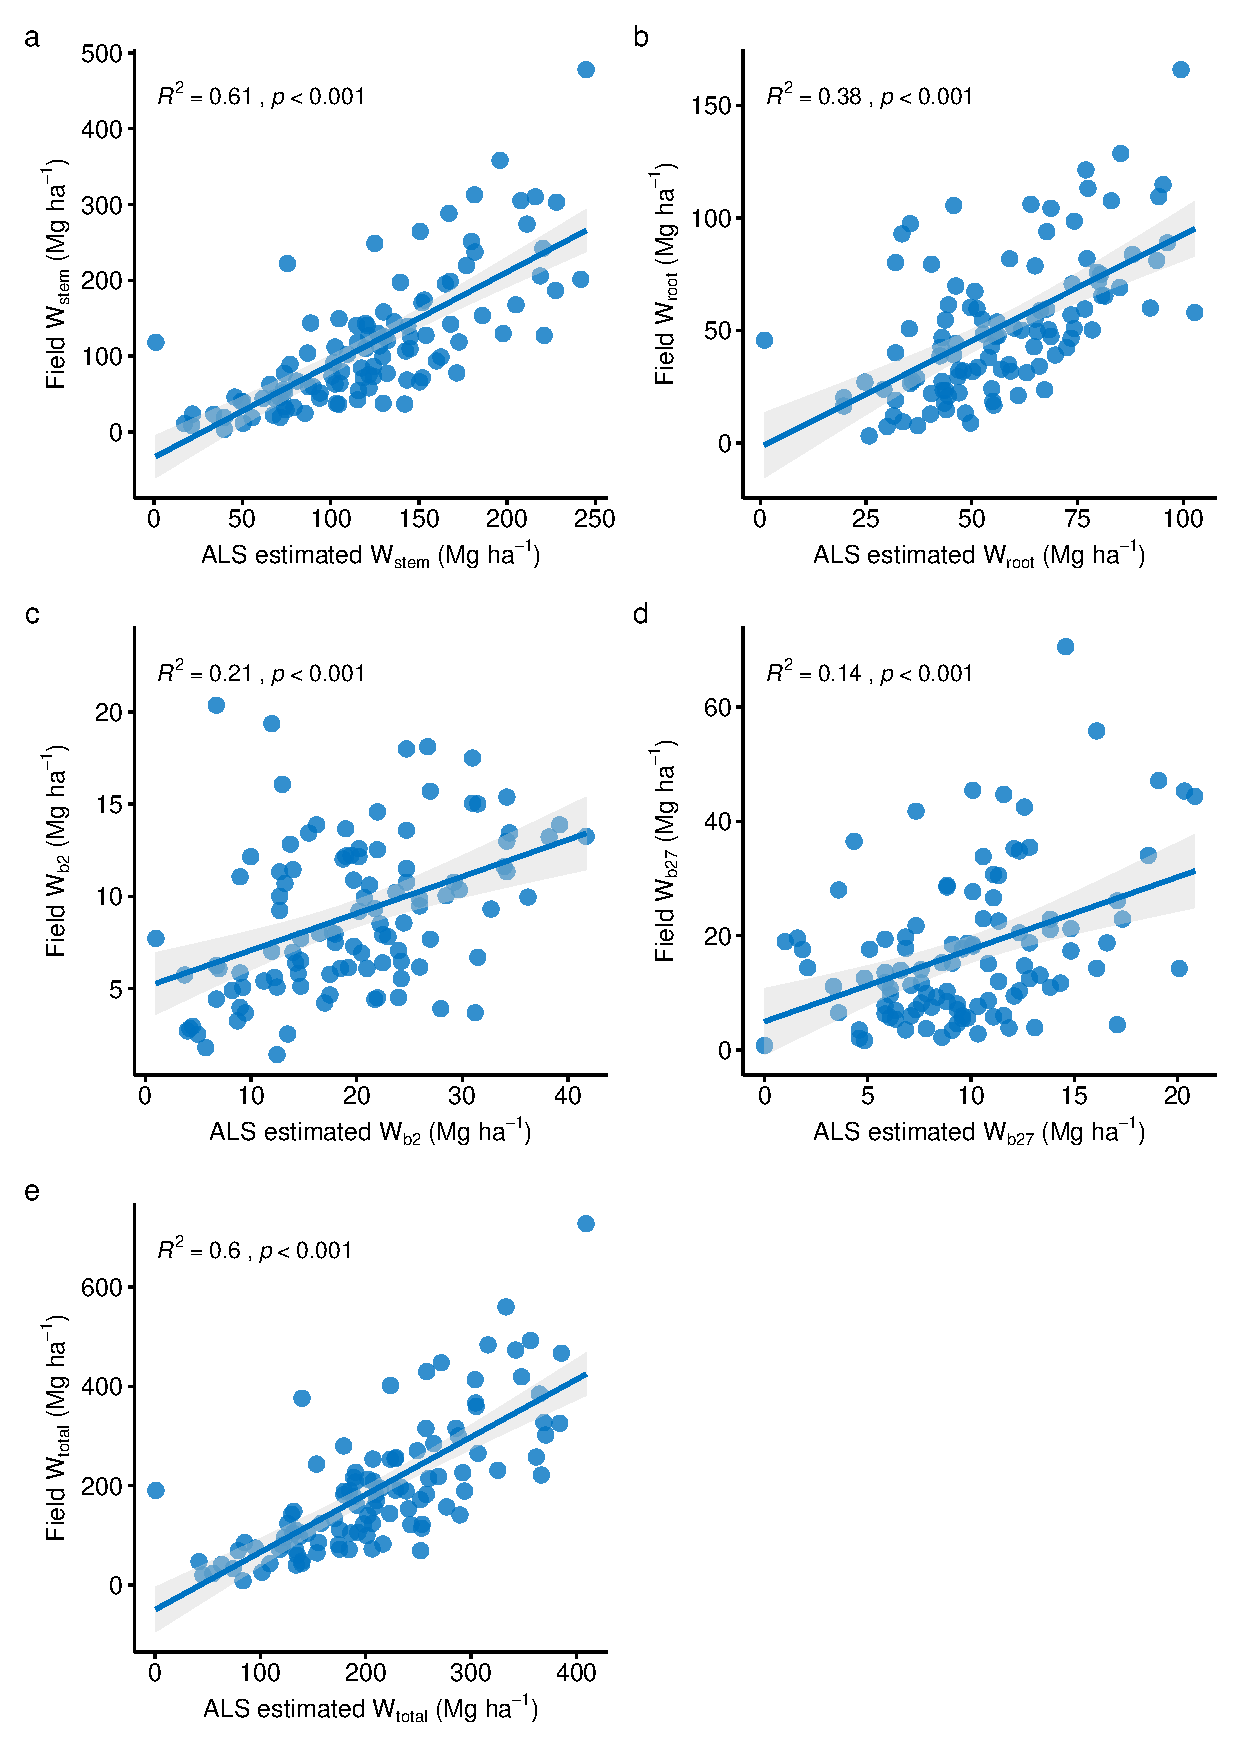
\includegraphics[height=.6\textheight]{img/carbon/carbon-compara-lidar-field.pdf}\caption{Scatterplots of the field-measured biomass fractions and the most accurate model-estimated values of the biomass fractions in the same plot. R\textsuperscript{2} and significance values of the correlation are included}\label{fig:carbon:compara}
\end{figure}

\begin{sidewaystable} 
\caption{Stand characteristics, field-measured and ALS-derived biomass (\mgha) and potential carbon dioxide sequestration (Mg CO$_2$ ha$^{-1}$) values for Pyrenean oak-population clusters in Sierra Nevada. Statistics and significance value for Kruskal-Wallis tests were shown. Different letters indicate statistically significant differences between oak-population clusters (Dunn's test, p < 0.05). Total values of ALS-derived Biomass (Mg) and Potential CO$_2$ sequestration (Mg CO$_2$) for all \Qp forests in Sierra Nevada are shown. Values in bracket show total values for each oak-population cluster.}\label{tab:carbon:compara}
\begin{adjustbox}{width=\linewidth}
	\begin{threeparttable}
		\begin{tabular}{lclclclrrr} 

\textbf{\emph{Stand features}} & \textbf{N} & ~ & \textbf{NW} & ~ & \textbf{S} & \textit{~} & \textit{Statistic} & \textit{p-value} &  \\ 
\toprule
Tree height (avg.) & 14.69 ± 0.81 a & ~ & 9.10 ± 0.55 b & ~ & 7.81 ± 0.36 b & ~ & 15.23 & \textit{\textless{}0.001} &  \\ 
Tree height (min) & 10.32 ± 1.49 a & ~ & 4.02 ± 0.52 b & ~ & 3.71 ± 0.31 b & ~ & 11.20 & \textit{0.004} &  \\ 
Tree height (max) & 18.54 ± 0.68 a & ~ & 14.76 ± 0.40 b & ~ & 13.89 ± 0.33 b & ~ & 12.67 & \textit{0.002} &  \\ 
DBH & 39.36 ± 6.00 a & ~ & 20.18 ± 1.24 b & ~ & 20.88 ± 1.54 b & ~ & 8.43 & 0.015 &  \\ 
Basal Area & 35.99 ± 6.61 a & ~ & 28.08 ± 2.34 a & ~ & 28.81 ± 2.26 a & ~ & 1.31 & 0.518 &  \\ 
Tree density & 405.51 ± 165.87 a & ~ & 898.86 ± 104.02 a & ~ & 838.35 ± 106.01 a & ~ & 3.69 & 0.158 &  \\ 
\midrule
\textbf{\emph{Field-measured biomass}} &  & ~ &  & ~ &  & ~ &  &  &  \\ 
\ws & 182.89 ± 33.18 & ~ & 113.21 ± 11.41 & ~ & 117.18 ± 11.72 & ~ & 4.30 & 0.116 &  \\ 
\wbs  & 28.82 ± 5.37 & ~ & 17.49 ± 1.85 & ~ & 17.31 ± 1.69 & ~ & 5.25 & 0.072 &  \\ 
\wb  & 8.75 ± 2.06 & ~ & 9.73 ± 0.74 & ~ & 8.63 ± 0.48 & ~ & 1.06 & 0.587 &  \\ 
\wro  & 65.52 ± 12.04 & ~ & 51.12 ± 4.26 & ~ & 52.46 ± 4.11 & ~ & 1.31 & 0.518 &  \\ 
\midrule
\textbf{\emph{ALS-derived measured}} &  & ~ &  & ~ &  & ~ &  &  & \textbf{\emph{Total}} \\ 
\ws & 84.29 ± 0.50 a (1.03 10$^6$) & ~ & 83.35 ± 0.37 a (1.98 10$^6$) & ~ & 89.16 ± 0.33 b (2.62 10$^6$) & ~ & 2296.42 & \textit{\textless{}0.001} & 5.62 10$^6$ \\
\wbs & 8.71 ± 0.04 a (0.10 10$^6$) & ~ & 8.24 ± 0.03 b (0.18 10$^6$) & ~ & 8.37 ± 0.02 c (0.24 10$^6$) & ~ & 1446.20 & \textit{\textless{}0.001} & 0.52 10$^6$ \\
\wb  & 13.16 ± 0.08 a (0.16 10$^6$) & ~ & 13.10 ± 0.06 a (0.31 10$^6$) & ~ & 14.18 ± 0.05 b (0.42 10$^6$) & ~ & 2138.11 & \textit{\textless{}0.001} & 0.89 10$^6$ \\
\wro  & 49.32 ± 0.21 a (0.59 10$^6$) & ~ & 46.56 ± 0.16 b (1.08 10$^6$) & ~ & 47.74 ± 0.13 c (1.4 10$^6$) & ~ & 2978.22 & \textit{\textless{}0.001} & 3.07 10$^6$ \\
\wt & 152.06 ± 0.81 a (1.85 10$^6$) & ~ & 147.27 ± 0.60 b (3.48 10$^6$) & ~ & 157.13 ± 0.53 c (4.61 10$^6$) & ~ & 2369.70 & \textit{\textless{}0.001} & 9.94 10$^6$ \\
CO$_2$ stock stem & 146.93 ± 0.86 a (1.03 10$^6$) & ~ & 145.30 ± 0.64 a (1.89 10$^6$) & ~ & 155.44 ± 0.57 b (2.44 10$^6$) & ~ & 2296.42 & \textit{\textless{}0.001} & 5.36 10$^6$ \\
CO$_2$ stock b27 & 15.19 ± 0.06 a (1.79 10$^6$) & ~ & 14.37 ± 0.05 b (3.44 10$^6$) & ~ & 14.59 ± 0.04 c (4.57 10$^6$) & ~ & 1446.20 & \textit{\textless{}0.001} & 9.8 10$^6$ \\
CO$_2$ stock b2 & 22.95 ± 0.15 a (0.28 10$^6$) & ~ & 22.85 ± 0.11 a (0.54 10$^6$) & ~ & 24.73 ± 0.10 b (0.73 10$^6$) & ~ & 2138.11 & \textit{\textless{}0.001} & 1.54 10$^6$ \\
CO$_2$ stock root & 85.98 ± 0.37 a (0.17 10$^6$) & ~ & 81.17 ± 0.27 b (0.31 10$^6$) & ~ & 83.23 ± 0.22 c (0.42 10$^6$) & ~ & 2978.22 & \textit{\textless{}0.001} & 0.9 10$^6$ \\
CO$_2$ stock total & 265.07 ± 1.41 a (3.22 10$^6$) & ~ & 256.72 ± 1.05 b (6.07 10$^6$) & ~ & 273.91 ± 0.93 c (8.04 10$^6$) & ~ & 2369.70 & \textit{\textless{}0.001} & 17.33 10$^6$ \\
\bottomrule
\end{tabular}
	\end{threeparttable}
\end{adjustbox}
\end{sidewaystable}

\subsection{Differences on biomass and C stock among Pyrenean oak  populations}\label{sec:carbon:results-cartography}
The cartography for total biomass (\wt) and the potential dioxide carbon sequestration of are shown in \figref{fig:carbon:mapas-wt}. The total estimated biomass (aboveground and belowground) existing in the \Qp woodlands of Sierra Nevada amounted to 9.94 Tg (1 Tg = 10$^12$ g), which represents a potential sequestration of 17.33 Tg of CO\textsubscript{2} (\tabref{tab:carbon:temporal}).

The spatial distribution of the estimated biomass in the \Qp forests of Sierra Nevada showed a general pattern with higher values mostly concentrated at southernmost oak woodlands. We observed that the MON population, belonging to NW cluster, showed the higher values for the estimated biomass and for the dioxide carbon sequestration potential (\figref{fig:carbon:mapas-wt}; \tabref{tab:carbon:biomass-pop}).

\begin{figure}
    \centering
    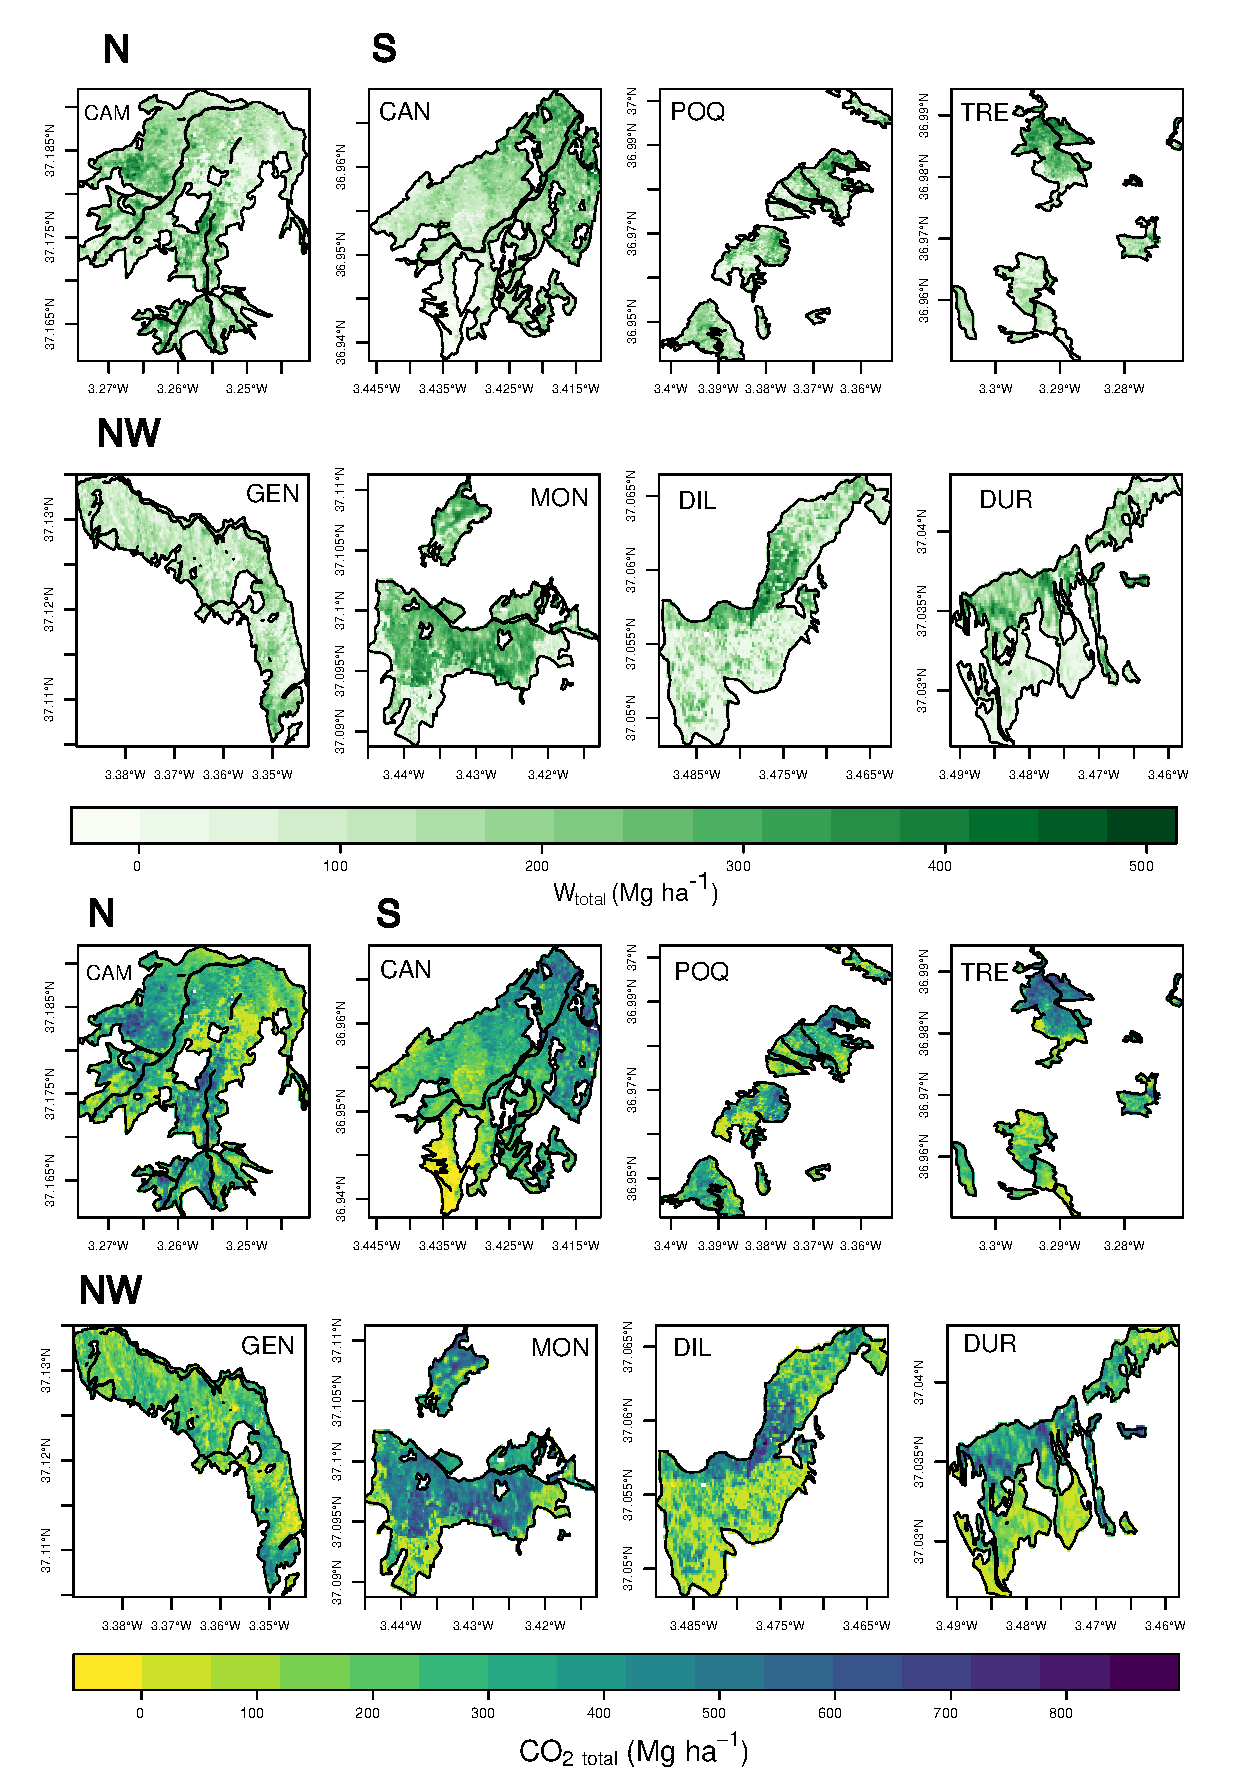
\includegraphics[width=\textwidth]{img/carbon/carbon-mapas-wt-ct.pdf}
    \caption{Total biomass (\wt) (\textbf{a}) and Potential Carbon sequestration (\textbf{b}) for each of the eight Pyrenean oak populations of Sierra Nevada. Different spatial scales were used for ease of visualization.}
    \label{fig:carbon:mapas-wt}
\end{figure}

The comparison of field-derived measures between oak-cluster populations revealed differences for tree height and DBH, but no for Basal Area and Tree density (\tabref{tab:carbon:compara}). The oak woodlands of N-cluster showed significantly taller trees with larger DBH than those of the NW and S (\tabref{tab:carbon:compara}, \figref{fig:carbon:schema}). Lower tree density and higher basal area were observed for N oak-woodlands, but the differences were not significant with the other oak-populations. No differences were found for field-biomass estimation between oak-populations (\tabref{tab:carbon:compara}).

\begin{sidewaystable} 
\caption{Summary of the best model (in terms of Bayesian Information Criterion) of total (\wt), stem (\ws), and root (\wro) biomass (\mgha) as a function of field-plot variables.}
\label{tab:carbon:bestmodels}
\begin{adjustbox}{width=\linewidth}
	\begin{threeparttable}
		\begin{tabular}{@{}l|crr|crr|crr@{}} \toprule
 & \textbf{\wt} &  &  & \textbf{\ws} &  &  & \textbf{\wro} &  &  \\ 
\textbf{\emph{Effects}} & \textbf{\emph{Estimate}} & \textbf{\emph{Z-value}} & \textbf{\emph{p-value}} & \textbf{\emph{Estimate}} & \textbf{\emph{Z-value}} & \textbf{\emph{p-value}} & \textbf{\emph{Estimate}} & \textbf{\emph{Z-value}} & \textbf{\emph{p-value}} \\ \toprule
Intercept & -1094.19 ± 292.09 & -3.75 & \textless{}0.001 & -721.44 ± 188.25 & -3.83 & \textless{}0.001 & -224.74 ± 68.09 & -3.3 & 0.001 \\
\textbf{$Ln$ Tree density (trees ha$^{-1}$)} & 102.04 ± 44.97 & 2.27 & 0.03 & 73.14 ± 28.98 & 2.52 & 0.01 & 22.08 ± 10.48 & 2.11 & 0.04 \\
\textbf{Elevation (m)} & 0.31 ± 0.05 & 6.77 & \textless{}0.001 & 0.17 ± 0.03 & 5.83 & \textless{}0.001 & 0.07 ± 0.01 & 6.83 & \textless{}0.001 \\
\textbf{Structural diversity index} & 2617.14 ± 828.65 & 3.16 & 0.002 & 1809.87 ± 534.06 & 3.39 & 0.001 & 542.41 ± 193.18 & 2.81 & 0.006 \\
\textbf{$Ln$ Tree density $\times$ Structural diversity index} & -349.22 ± 122.01 & -2.86 & 0.005 & -242.94 ± 78.63 & -3.09 & 0.003 & -76.26 ± 28.44 & -2.68 & 0.009 \\ \midrule
\textbf{Degree of freedom} & 101 &  &  & 101 &  &  & 101 &  &  \\
\textbf{AIC} & 1196 &  &  & 1103 &  &  & 887 &  &  \\
\textbf{BIC} & 1212 &  &  & 1119 &  &  & 903 &  &  \\
\textbf{Deviance Explained} & 0.413 &  &  & 0.373 &  &  & 0.381 &  &  \\ \bottomrule
\end{tabular}
\end{threeparttable}
\end{adjustbox}
\end{sidewaystable}

Significant differences for ALS-estimated biomass were found among oak-clusters (\tabref{tab:carbon:compara}). The values for the stem fraction (\ws) and small branches (\wb) biomass fractions were significantly higher for S oak-populations than for those in the N and NW, the latter showing no differences (\tabref{tab:carbon:compara}). The total biomass (\wt) was significantly different between oak-population clusters with higher values for southern oak populations (\figref{fig:carbon:schema}). Root biomass (\wro) and medium branches biomass (\wbs) were significantly higher for northern oak-populations (N) (\tabref{tab:carbon:compara}; \figref{fig:carbon:schema}).

\begin{figure}
    \centering
    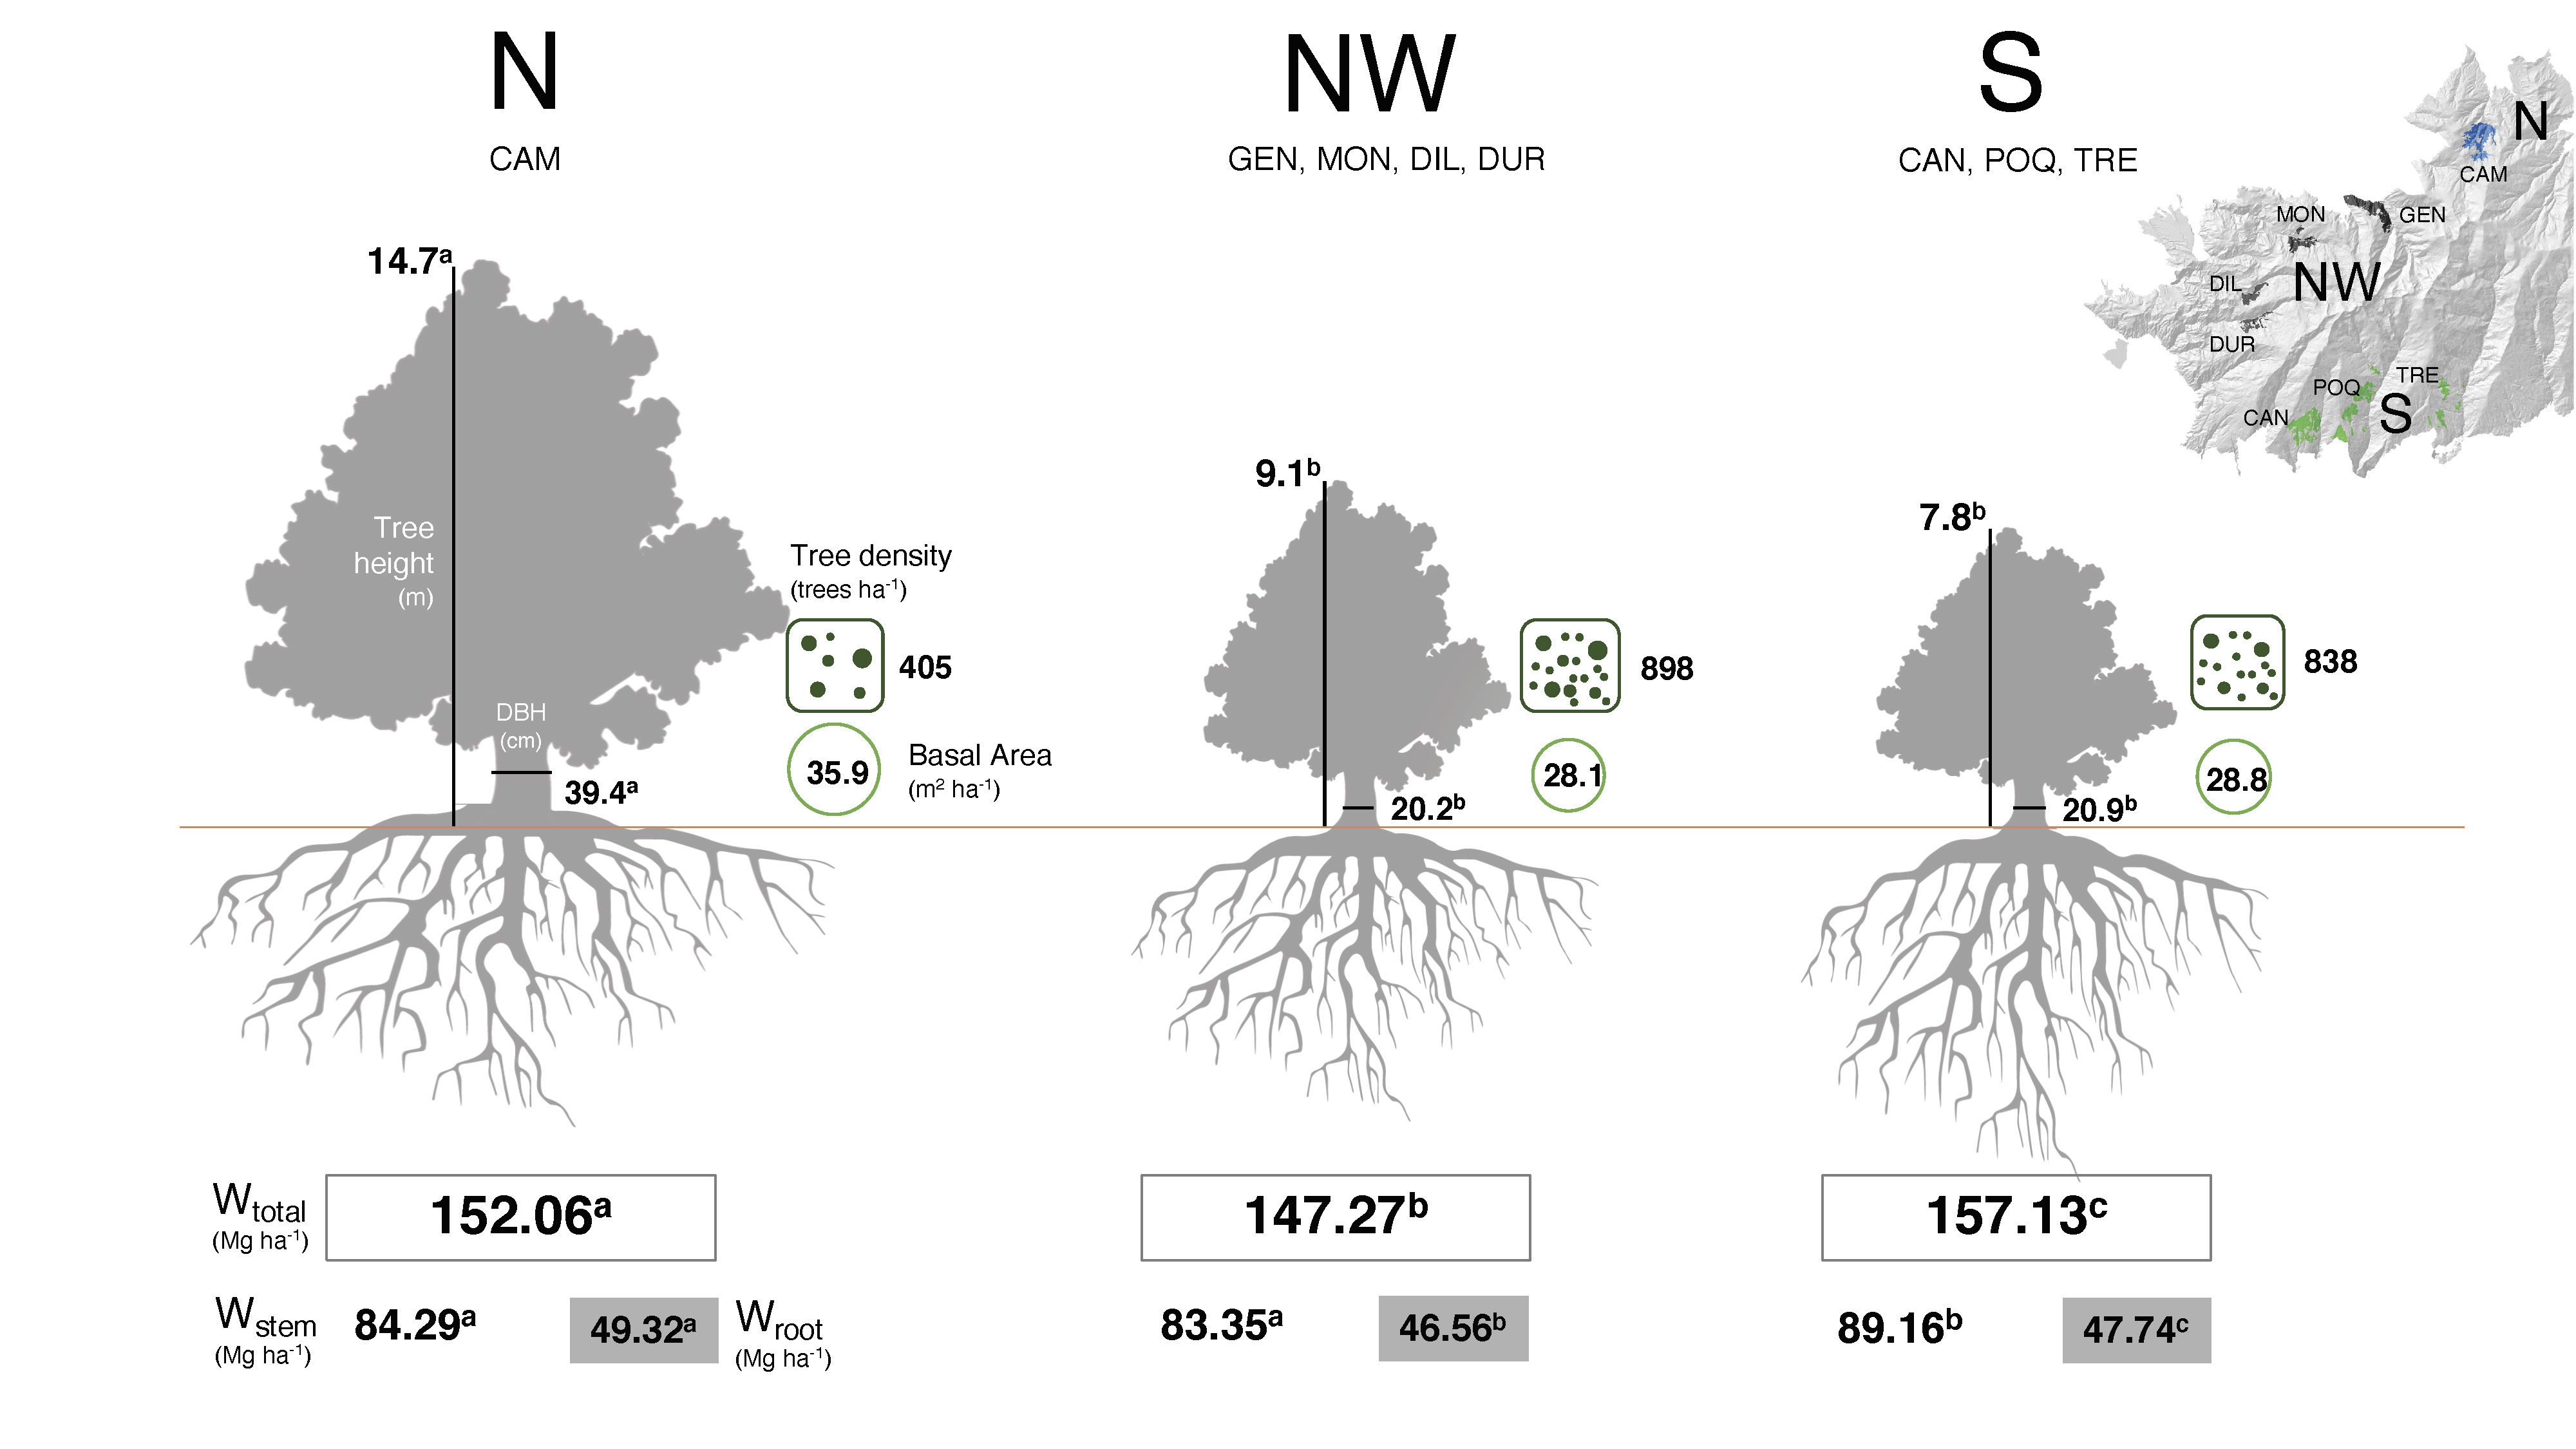
\includegraphics[width=\textwidth]{img/carbon/carbon-esquema-compara2.jpg}
    \caption{Comparison of stand features and ALS-estimated biomass fractions between oak-population clusters of \Qpy woodlands in Sierra Nevada. The distribution of oak-cluster are shown upper-right. Different letters indicate statistically significant differences between oak-population clusters (Dunn's test, p \textless 0.05) after Kruskal-Wallis test.}
    \label{fig:carbon:schema}
\end{figure}

\subsection{Predictions of Stand Biomass}\label{sec:carbon:results-prediction}
The best GLM models selected for total (\wt), stem (\ws) and root (\wro) biomass explained 70.3\%, 67.3\% and 63.1\% of variance respectively (\tabref{tab:carbon:bestmodels} and \tabref{tab:carbon:model-selection}). The elevation and the shannon structural diversity index showed positive effects on estimated biomass (\tabref{tab:carbon:bestmodels}; \figref{fig:carbon:glm}). Tree density negatively affected the estimated total biomass. The interaction between tree density and the shannon structural diversity index was significantly (\tabref{tab:carbon:bestmodels}), indicating that the total biomass increased with the increase structural diversity at lowest and medium tree densities, but decreased at high values of tree density (\figref{fig:carbon:glm}).

\begin{figure}
    \centering
    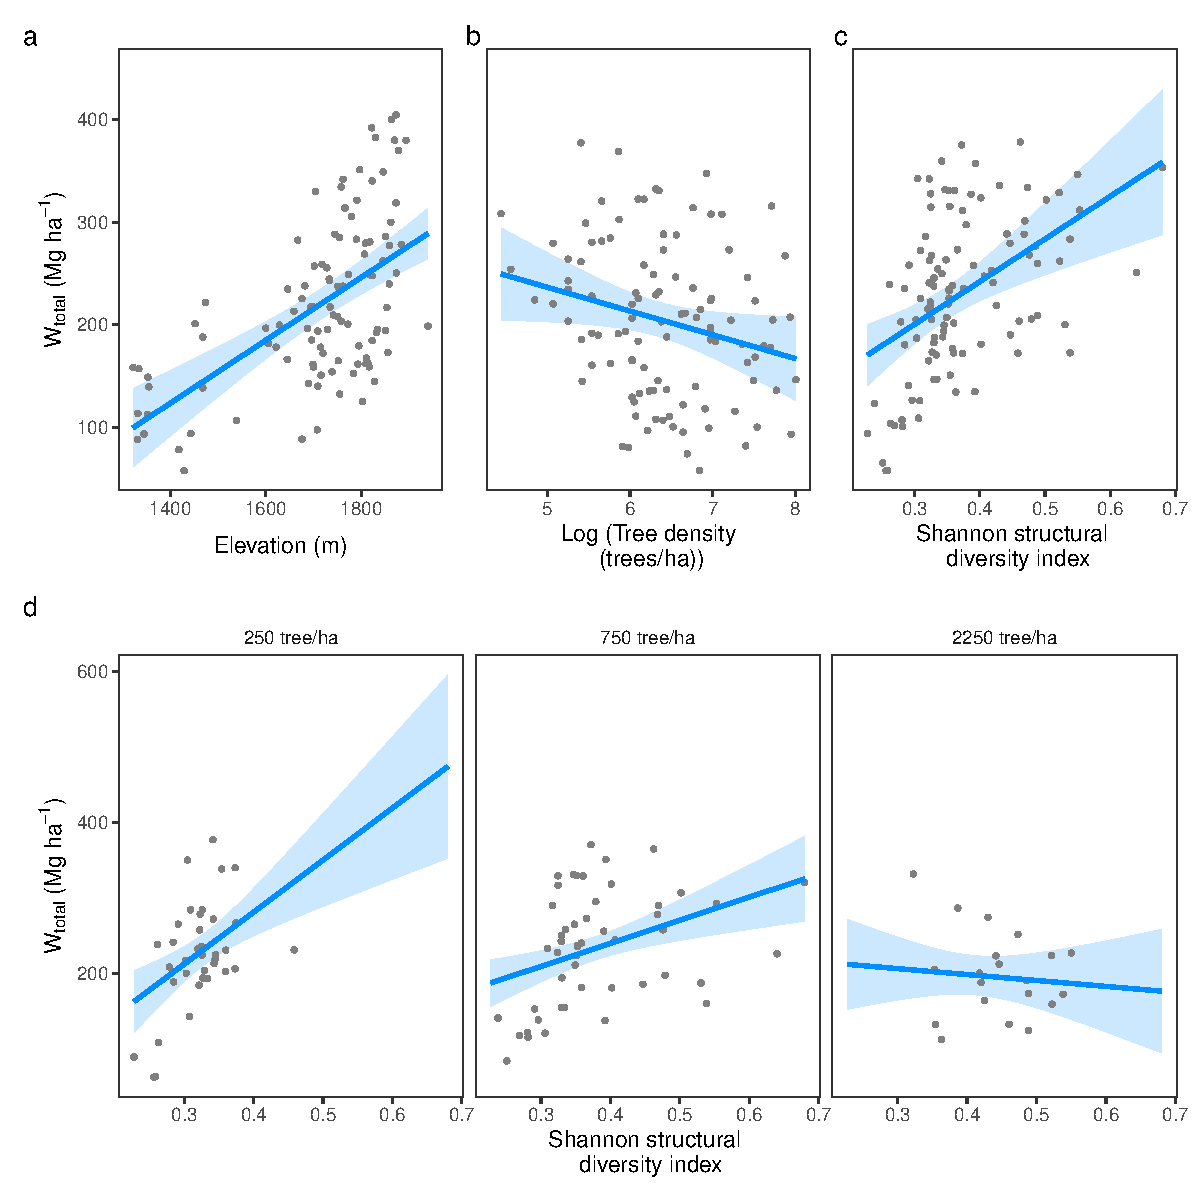
\includegraphics[width=\textwidth]{img/carbon/carbon-glm-effects.pdf}
    \caption{Predicted effects of the (\textbf{a}) elevation (meters), (\textbf{a}) tree density (trees ha\textsuperscript{-1}), (\textbf{c}) shannon structural diversity index, and (\textbf{d}) tree density $\times$ shannon structural diversity index, on the total biomass (\wt; \mgha).}
    \label{fig:carbon:glm}
\end{figure}


\subsection{Temporal evolution of Biomass in \Qp stands}\label{sec:carbon:results-temporal}
A general pattern of increase in aboveground tree biomass was observed for most analyzed plots (\tabref{tab:carbon:temporal}), with a total increase of 19 172 \mgha between the two national forest inventories. About 89 \% of the plots showed an increase in aboveground tree biomass, with an average of 11.46 \mgha (\tabref{tab:carbon:temporal}). This general pattern was also observed for plots located in Sierra Nevada (\figref{fig:carbon:ifn}).

\begin{figure}
    \centering
    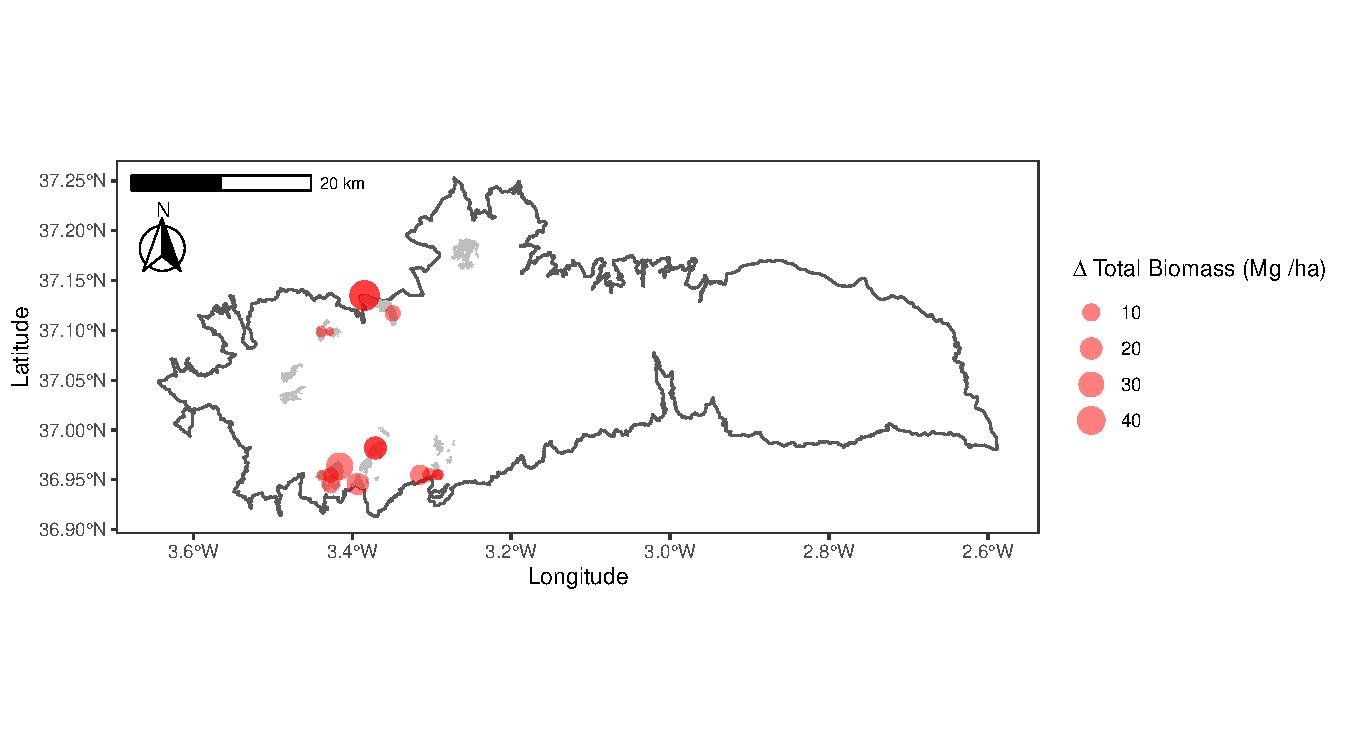
\includegraphics[width=\textwidth]{img/carbon/carbon-mapa-ifn.pdf}
    \caption{Variation of tree biomass between the second and third Spanish National Forest Inventories, for plots (points) located on Sierra Nevada which have \Qp as the main species. Size point indicates the variation in total biomass ($\Delta$ \mgha).}
    \label{fig:carbon:ifn}
\end{figure}

\begin{table}[]
\caption{Temporal evolution of the total biomass (\mgha) of \Qp and the total carbon (\mgha) between the second (SNFI2) and third (SNFI3) Spanish National Forest Inventories. Plots were aggregated by loss/gains of the tree numbers ($\Delta$ trees), and also by increase/decrease of biomass during the period analyzed. The total variation in biomass (\emph{i.e.} sum for all plots), and the average variation per plot are shown for each category. }
\footnotesize
\label{tab:carbon:temporal}
\resizebox{\textwidth}{!}{%
\begin{tabular}{clc|>{\centering}p{2cm}|>{\centering}p{3cm}|c}
\toprule
$\Delta$ \textbf{trees} & \textbf{Biomass} & \textbf{\# plots} & $\Delta$ \textbf{total biomass (\mgha)} & \textbf{Average  variation per plot (\mgha)} & \textbf{ Total Carbon} \tabularnewline \toprule
\multirow{2}{*}{\textless 0} & Decrease & 159 & -1060.39 & -6.67 (0.86) & -1846.85 \tabularnewline
 & Increase & 123 & 921.40 & 7.49 (0.86) & 1604.77 \tabularnewline \midrule
\multirow{2}{*}{\textgreater 0} & Decrease & 33 & -287.19 & -8.7 (2.82) & -500.19 \tabularnewline
 & Increase & 1586 & 18183.25 & 11.46 (0.41) & 31669.16 \tabularnewline \midrule
\multirow{2}{*}{0} & Decrease & 56 & -141.40 & -2.53 (0.59) & -246.28 \tabularnewline
 & Increase & 312 & 1556.16 & 4.99 (0.48) & 2710.32 \tabularnewline
 \bottomrule
\end{tabular}%
}
\end{table} 
\normalsize

\section{Discussion}\label{sec:carbon:discussion}
\subsection{Carbon sequestration by Sierra Nevada oak woodlands.}\label{sec:carbon:discussion-sn}

Total estimated biomass values in Sierra Nevada oak woodlands ranged from 147.27 -- 157.13 \mgha (\tabref{tab:carbon:compara}), with aboveground biomass (sum of \ws, \wb and \wbs fractions) ranging from 104.69 - 111.71 \mgha. Our results are consistent with the mean aboveground biomass density cited by the IPCC guidelines as the default value for temperate mountain systems (130 (20 - 600) \mgha) in Europe \autocite{IPCC2006ForestLand}. Using data from the Spanish Third National Forest Inventory, \citet{Vayredaetal2012SpatialPatterns} reported an average value for stand C stock of 45 \mgha along the distribution of \Qp in the Iberian Peninsula. Those values were lower than the estimated carbon stock (above- and below-ground) in our study which ranged from 69.95 - 74.63 \mgha (\tabref{tab:carbon:compara}). At a more regional scale, our results showed higher values than those found in the central range of the species distribution, where aboveground biomass varied between 63.8 - 98 \mgha \autocite{GallardoLanchoGonzalezHernandez2004SequestrationCarbon}. Estimates of dioxide carbon sequestration for \Qp pure stands (122.19 - 152.82 \mgha) located in the Central Mountain Range (Spain) \autocite{Canellasetal2008SilvicultureCarbon,Canellasetal2017CarbonSequestration} were also lower than our results (256.72 - 273.91) (\tabref{tab:carbon:compara}). Despite the potential differences derived from the carbon estimation method (\emph{i.e.} LIDAR estimation \emph{versus} field-ground based estimation; biomass expansion factors), several factors could explain the differences found in our results with respect to the values reported for other studies. First, it is generally accepted that there is an age‐related decline in stand biomass accumulation \autocite[ and references therein]{Xuetal2012AgerelatedDecline} with the productivity of old-growth forests being usually lower than younger forests \autocite{Kutschetal2009EcophysiologicalCharacteristics}. Oak woodlands of Sierra Nevada are composed of relatively young trees \autocite{GeaIzquierdoCanellas2014LocalClimate,PerezLuqueetal2020LanduseLegacies,RubioCuadradoetal2018AbioticFactors} in comparison with other woodlands of the species along their distribution area \autocite{GeaIzquierdoCanellas2014LocalClimate}. The strong anthropic perturbations in these oak has conditioned their structure. For instance, some of the oak woodlands were massively cut down during Spanish Civil post-war period for use as wood gas for vehicles \autocite[\emph{e.g.} MON population;][]{Prieto1975BosquesSierra}, or for use in intense mining activities \autocite[\emph{e.g.} GEN population;][]{PerezLuqueetal2020LanduseLegacies}. Therefore, we can consider that many of the oak woodlands of Sierra Nevada oaks are relatively young, which might explain the high potential for C accumulation obtained in our study, since it has been shown that forest created as a result of drastic land-use changes exhibited faster growing rates, and therefore higher potential C accumulation, than pre-existing forests \autocite{VilaCabreraetal2017NewForests}. Differences in carbon stock between young oak coppices and mature forests were reported for other \emph{Quercus} species \autocite{Bruckmanetal2011CarbonPools,Cotillasetal2016AbovegroundBelowground}. Therefore, it is likely that the high total ecosystem C values obtained in our area of study could be partly explained by the stands age-development stage \autocite{Makinecietal2015EcosystemCarbon}. Secondly, the water availability is generally the most limiting factor driving radial growth of \Qp along its distribution range in the Iberian Peninsula \autocite{GeaIzquierdoCanellas2014LocalClimate}. In Sierra Nevada, northern and northwestern oak populations are located in valley bottoms with high values of relative humidity; and southern ones get the extra supply of water from moist air from the Mediterranean sea. Therefore water availability does not seem to be strongly limiting the oak-growth in this mountain region. In fact, in the last decades positive trends have been observed for greenness and secondary growth of oak woodlands in Sierra Nevada \autocite{GeaIzquierdoCanellas2014LocalClimate,PerezLuqueetal2020LanduseLegacies,RubioCuadradoetal2018AbioticFactors} suggesting that this mountain range could act as an ecological refugee for this species. Thus those positive growth trends could explain the high values of carbon sequestration obtained in our study.

\subsection{Factors explaining biomass in the oak woodlands}\label{sec:carbon:discussion-factors}
Regarding the factors explaining biomass, we found a positive effect of the structural richness on total biomass, and therefore on C stock (\figref{fig:carbon:glm}). Our results are consistent with general patterns obtained for tree species in Iberian Peninsula \autocite{Vayredaetal2012SpatialPatterns}. In structural-heterogeneous stands, trees occupy different horizontal and vertical layers, thus they can maximize the resources \autocite[\emph{e.g.} light][]{Forrester2014StandlevelLight}, whereas homogeneous stand structure may reduce complementary effects \autocite{Goncalves2018EffectsForest,Vayredaetal2012SpatialPatterns}. Being surrounded by size-diverse neighbours allow trees to fill the available canopy space around them and hence capture more light \autocite{Forrester2014StandlevelLight,Vanhellemontetal2018SpeciesStructural}. Our results show that the higher the tree density, the lower the total biomass (\figref{fig:carbon:glm}).
Previous studies on forests located on NW of Spain, reported tree stand density as one of the main factors affecting potential biomass production and carbon sequestration \autocite{CastanoSantamariaetal2013PotentialGround}. Tree growth of \Qp is inversely influenced by competition \autocite{Canellasetal2004GrowthResponse,FernandezdeUnaetal2015StandCompetition,FernandezdeUnaetal2016DisentanglingEffect}. Thus, trees respond to reduced competition through the structural shifts such as increased radial growth \autocite{Canellasetal2004GrowthResponse,FernandezdeUnaetal2016DisentanglingEffect}, and therefore a potential increase in biomass. We also found an interaction effect between the tree-density and stand structure diversity (\figref{fig:carbon:glm}) which suggests that at high tree-densities resources are not maximized, even if structural diversity exists.
Despite the importance of the water availability in the growth of \Qp \autocite{GeaIzquierdoCanellas2014LocalClimate,MorenoFernandezetal2020InfluenceClimate}, none of the best models selected for \wt, \ws or \wro, included the topographic wetness index (\tabref{tab:carbon:model-selection}). This would seem suggest that the water requirement of this species in this mountain is met by the location of the oak populations within Sierra Nevada, and therefore would reinforce the role of this mountain region as an ecological refugee for this species.

\subsection{Biomass differences within oak woodlands}\label{sec:carbon:discussion-differences}
We found that oak woodlands of the Northern cluster showed stands with taller and greater trees (\tabref{tab:carbon:compara}), and also high values of biomass (Figures \ref{fig:carbon:mapas-wt} and \ref{fig:carbon:schema}). It could be related with lower intensity of anthropogenic disturbances in comparison with the other oak woodlands, mainly because the northern oak woodlands had greater protection during the second half of the last century \autocite{JimenezOlivencia1991PaisajesSierra}, and currently also have the highest level of legal protection within the protected area \autocite{Anonymous2011Decreto238}. The less anthropogenic disturbances have resulted in well-conserved forests with a greater species diversity \autocite{PerezLuqueetal2021EcologicalDiversity}, and also a stable stand structure with high values of biomass (Figures \ref{fig:carbon:mapas-wt} and \ref{fig:carbon:schema}). For other species of \emph{Quercus} it has been observed that forests with less disturbance have a higher potential for carbon storage \autocite{BalboaMuriasetal2006CarbonNutrient,Cotillasetal2016AbovegroundBelowground,Stojanovicetal2017ForecastingTree}.

Our results also highlighted how differences in stand structure conditioned stand tree biomass (\tabref{tab:carbon:bestmodels}, \figref{fig:carbon:glm}). High dense stands, \emph{i.e.} northwestern oak populations, showed lower total biomass than less dense stands (northern or southern oak populations) (\figref{fig:carbon:schema}). High stand density increase tree competition, limiting stand growth which provokes loss of vitality and reduction in acorn production \autocite{Bravoetal2008SelviculturaMontes,Piqueetal2018Spain}, and according to our results, the higher the tree density the lower the capacity of these forests to act as carbon sinks (Figures \ref{fig:carbon:schema}, \ref{fig:carbon:glm}). In addition, an accumulation of biomass, coupled with a loss of structural diversity (\figref{fig:carbon:glm}), would increase the risk of forest fires due to the large amount of biomass \autocite{Canellasetal2004GrowthResponse,PiqueVericat2015EvolutionPerspectives,Serradaetal1992CoppiceSystem}

\subsection{Trends of carbon sequestration by oak woodlands}\label{sec:carbon:discussion-trends}
We observed an increase in aboveground tree biomass between the two inventories for plots located in oak woodlands (\tabref{tab:carbon:temporal}, \figref{fig:carbon:ifn}). Recent studies have reported a positive trend for primary production and for secondary growth in oak woodlands in Sierra Nevada \autocite{AlcarazSeguraetal2016ChangesVegetation,Dionisioetal2012SatelliteBasedMonitoring,PerezLuqueetal2015OntologicalSystem,PerezLuqueetal2020LanduseLegacies}. In addition, an increase in the area occupied by oak forests \autocite{CamachoOlmedoetal2002TransformacionPaisaje} as well as the densification of existing forest have been found \autocite{JimenezOlivenciaetal2015MedioSiglo}. All these results indicated that this ecosystem service, \emph{i.e.} carbon sequestration, have suffered an increase in the last decades in our study area. Land-use changes have extensively affected C storage of terrestrial ecosystems for several areas of south Europe \autocite{MunozRojasetal2011ChangesLand,MunozRojasetal2015ImpactLand}. Abandonment of traditional activities and rural exodus are the main drivers explaining the densification and expansion of forests particularly in mountainous regions such as Sierra Nevada \autocite{JimenezOlivenciaetal2015MedioSiglo,MacDonaldetal2000AgriculturalAbandonment}. Considering the positive trend observed for the increase in biomass, and the lack of direct human-drive disturbances as these forests are in a protected area, it would expect a positive trend in forest carbon stock, such as has been recorded in many forests in the Mediterranean region in the last decades \autocite{FAOPlanBleu2018StateMediterranean}. It also agrees with the predictions under different scenarios forecasting a forest growth in the next decades \autocite{Aparicioetal2015ClimateChange}. However, it should be taken with caution, since some early signs of saturation of forests as a carbon sink are being documented in Europe \autocite{Nabuursetal2013FirstSigns}.

\section{Management implications}\label{sec:carbon:discussion-management}

Several studies indicated that reductions of tree-density on oak coppices forests, by moderate thinning, causes an increase in the tree growth and biomass for \Qp woodlands \autocite{Aldeaetal2017ThinningEnhances,Aldeaetal2017EfectoClaras,MorenoFernandezetal2020InfluenceClimate,Canellasetal2004GrowthResponse}, and also for other \emph{Quercus} species \autocites[\emph{e.g.}][]{Cotillasetal2009GrowthResponse,FernandezdeUnaetal2015StandCompetition}. This reduction in the stand density could increase the carbon sequestration of the woodland by a higher structural diversity which maximized the use of resources \autocite{CastanoSantamariaetal2013PotentialGround}. Esta reducción de la densidad, además implica una menor cantidad de biomasa de pequeño tamaño, mejorando las condición fuegos 
% !TEX root = ../my-thesis.tex
%
\selectlanguage{english}  
\chapter{\textcolor{ctcolormain}{Land-use legacies and climate change as a double challenge to oak forest resilience: mismatches of geographical and ecological rear edges}}\label{sec:dendro}

\mbox{}
\vfill
{\color{ctcolormain}\textbf{Antonio J. Pérez-Luque}}; Guillermo Gea-Izquierdo \& Regino Zamora. 2020. \emph{Ecosystems}  \href{https://doi.org/10.1007/s10021-020-00547-y}{10.1007/s10021-020-00547-y}

\newpage

\paragraph{Abstract} \mbox{} \\
Global change challenges ecosystems in xeric locations transformed by intensive human use. Resilience to drought of relict Mediterranean \Qpy populations in the southern Iberian Peninsula was analyzed in relation to historical records of land use, combining dendroecological growth of adult trees and greenness (EVI) as proxies for secondary and primary growth. The growth trends reflected a strong influence of old land-use legacies (\emph{e.g}. firewood removal) in the current forest structure. Trees were highly sensitive to moisture availability, but both primary growth and secondary growth expressed high resilience to drought events over the short and the long term. Resilience and the tree growth response to climate followed a water-stress gradient. A positive growth trend since the late 1970s was particularly evident in mesic (colder and wetter) high-elevation stands, but absent in the most xeric (warmer and drier) stands. The high values of resilience observed suggest that the studied \Qp populations are located in a geographical but not a climatic or ecological rear edge. Resilience of oak stands to drought events was not spatially homogeneous across the mountain range, due to differences in ecological conditions and/or past management legacies. This is particularly relevant for rear-edge populations where topographic and biophysical variability can facilitate the existence of refugia.

\newpage

\section{Introduction}\label{sec:dendro:Intro}

The response of species to changing environments (\emph{e.g.} distributional shifts) can be determined largely by population responses at range margins \autocite{HampePetit2005ConservingBiodiversity}. Peripheral populations are usually considered more vulnerable compared with populations at the center of a species' range {[}\emph{i.e.} center-periphery hypothesis; \textcite{SagarinGaines2002AbundantCentre}; \textcite{Pirononetal2017GeographicVariation}{]}. Geographically marginal populations have often been assumed to represent ecologically marginal populations. This means lower performance, higher vulnerability, and thus higher risk of extinction than for populations at the core of the species' range \autocite{Rehmetal2015LosingYour,Pirononetal2017GeographicVariation,VilaCabreraetal2019RefiningPredictions}. Nonetheless, recent reviews report that species- and population-specific responses do not always support this hypothesis \autocite{Sextonetal2009EvolutionEcology,Abelietal2014EffectsMarginality,Oldfatheretal2020RangeEdges}. This is partly because a rear-edge is a multidimensional concept including an ecological (\emph{i.e.} climatic and edaphic), a geographical, and a genetic component \autocite{VilaCabreraetal2019RefiningPredictions}, but also an anthropogenic dimension (\emph{i.e.} land-use). In this respect, to fully understand changes in distribution and abundance of species as a consequence of global change, it is crucial to identify and understand mismatches between the geographical and the ecological rear edges \autocite{VilaCabreraJump2019GreaterGrowth}.

Limits of species distribution are strongly determined by climatic factors and biotic interactions \autocite{Gaston2009GeographicRange,Sextonetal2009EvolutionEcology}. Climate change is expected to cause major shifts in the distribution and abundance of plant communities, and signs already indicate that more intense and longer droughts are altering forest dynamics \autocite{Allenetal2010GlobalOverview}. Drought frequency and severity have increased in recent decades, with a trend towards drier summers, particularly for Southern Europe \autocite{VicenteSerranoetal2014EvidenceIncreasing,Staggeetal2017ObservedDrought}. In this climatic-change context, population loss and range retractions are expected in boreal, temperate, and Mediterranean species at the lowest latitudes and elevations, as well as in drought-prone areas of a species' distribution, \emph{i.e.} the rear edge. The rear-edge populations are likely to be more sensitive to minor climatic and microtopographic variations and therefore the effects of droughts are expected to be particularly noteworthy \autocite{HampePetit2005ConservingBiodiversity,VilaCabreraetal2019RefiningPredictions}.

It is often overlooked that human activity constitutes a driver of change as powerful or even more powerful as natural drivers, \emph{i.e.} natural variation in climate, particularly for regions with long land-use history such as the Mediterranean Region \autocites[\emph{e.g.}][]{NavarroGonzalezetal2013WeightLanduse,DoblasMirandaetal2017ReviewCombination}. In these areas, the susceptibility and response of ecosystems to climate change are conditioned by legacies of historical land-use activity \autocites[\emph{e.g.}][]{Munteanuetal2015Legacies19th,Mausolfetal2018LegacyEffects}. The past land-use legacies interact with recent human-caused climate disturbances and may confound their interpretation \autocite{Fosteretal2003ImportanceLanduse}. For example, recent works showed that a quarter of current forests in the Iberian Peninsula, are growing on former agricultural and grazing land abandoned after the 1950s \autocite{VilaCabreraetal2017NewForests}. Consequently, anthropogenic habitat modification and its legacies represent a critical dimension of marginality as they may intensify, confound or delay climate-driven population decline at rear edges \autocite{VilaCabreraJump2019GreaterGrowth,SanchezdeDiosetal2020FagusSylvatica}. In this context, our work seeks to identify the impacts and responses to natural (\emph{e.g.} severe drought) and human disturbances (\emph{e.g.} logging) on oak forests at their southern geographical range. A historical perspective should help us to interpret the responses of ecosystems to disturbances \autocite{Fosteretal2003ImportanceLanduse}, particularly regarding marginal rear-edge populations \autocite{VilaCabreraetal2019RefiningPredictions}.

The assessment of resilience to climate and human disturbances provides critical information concerning the capacity of forests to maintain their structure and render valuable ecosystem services. Resilience is the capacity of an ecosystem to persist and maintain its state and functions in the face of disturbance \autocite{Holling1973ResilienceStability,Hodgsonetal2015WhatYou}. \textcite{Lloretetal2011ComponentsTree} proposed an approach, which decomposes resilience into three components: resistance to drought, recovery after drought and resilience. This resilience is determined by the forest's ability to mitigate the disturbance (resistance) and the capacity to recover from the impact (recovery) \autocite{IngrischBahn2018ComparableQuantification}. This conceptual approach has recently become widely used to assess forest resilience, because it allows a simple, yet highly efficient assessment of short-term responses of trees to drought. Nevertheless, not exempt from criticism, this approach needs to be applied carefully to avoid potential bias at different levels \autocite{Schwarzetal2020QuantifyingGrowth}. In this sense we assessed forest resilience both over the short-term to several recent extreme drought episodes, as well as over the long-term to climate change (\emph{i.e.} warming on the last few decades), using two different proxies to characterize resilience. Dendroecological estimates of growth (\emph{i.e.} tree-ring width) are commonly used proxies to characterize tree vitality and have commonly been used to study growth changes in response to drought at the individual tree level \autocite{Fritts1976TreeRings,Dobbertin2005TreeGrowth}. Remote sensing can be used to analyze the impact of drought on ecosystems at the stand level \autocite[\emph{e.g.}][]{Zhangetal2013MonitoringEstimating}. Tree-ring records complement remote-sensing data with a longer time scale. Tree rings can reflect tree-growth anomalies induced by climate or other disturbance over decades to centuries \autocite{Babstetal2017ImprovedTreering} and provide an accurate measure of growth responses to droughts \autocite{Bhuyanetal2017DifferentResponses}. The combination of remote sensing and dendroecology has been used to assess the effects of droughts on vegetation along ecological gradients \autocites[\emph{e.g.}][]{VicenteSerranoetal2013ResponseVegetation,Coulthardetal2017TreeGrowth}, and also to evaluate growth resilience to drought in several tree species \autocites[\emph{e.g.}][]{Gazoletal2018ForestResilience,PenaGallardoetal2018DroughtSensitiveness}.

In the present study, we assess resilience of \Qpy (Pyrenean oak) from southern relict forests at the rear edge of the species distribution, where species performance is considered to be threatened by climate change \autocite{GeaIzquierdoetal2013GrowthProjections,GeaIzquierdoetal2017RiskyFuture}. For this, we combined remote-sensing information and dendroecological methods to evaluate the impact of drought both on canopy greenness (as a proxy for primary growth) and radial tree growth (as a proxy for secondary growth). For the analysis of forest resilience to climate, we took into account the land-use history of these transformed forests, thoroughly reviewing historical documents to reconstruct forest history at the study sites, and analyzing how anthropogenic drivers have shaped the current forest structure. Based on this analysis, we developed a rationale that integrates the ecological and anthropogenic components of marginality to determine the regional and local scale mechanisms shaping the probability of persistence (or extinction) of rear-edge oak populations. Our main hypothesis is that range edge stands will show low resilience to extreme droughts, but that the vulnerability to drought will be reduced quickly across a fine-scale topographic gradient of decreasing aridity. To test this hypothesis, we: (\emph{i}) quantified how recent extreme drought events influenced primary and secondary growth of \Qp forests at their present geographical rear edge; (\emph{ii}) analyzed the long-term resilience of these forests to extreme drought events, using time-series of radial growth; (\emph{iii}) reviewed historical documents to reconstruct forest-management history and to infer how it impacted tree growth and stand dynamics over time; (\emph{iv}) and examined differences in the resilience metrics between populations under contrasting ecological conditions (\emph{i.e.} xeric \emph{vs.} mesic) along environmental gradients within the rear edge in order to detect vulnerability to climate change at the small spatial scale.

\begin{sidewaystable} 
\caption{Characteristics of sampled plot. Lat = latitude; Long = longitude. Dbh and height of all trees, Basal Area (BA), Density and SRD (size ratio proportional to distance) are computed for all trees within a 10-m radius of focal trees (see Materials and methods). Temp.: annual average of mean monthly minimum and maximum temperatures. Values shown here correspond to site averages. Standard deviations are shown in parentheses. Different letters indicate statistically significant differences between sites (Kruskal-Wallis test followed by Dunn's test, \emph{p<0.05}). Stands were monospecific, hence all results correspond to oak data.}\label{tab:dendro:sampledPlots}
\begin{adjustbox}{width=\linewidth}
\begin{threeparttable}
\begin{tabular}{p{1cm}p{1.2cm}p{1.2cm}p{2.3cm}p{1.3cm}p{1cm}p{1.3cm}p{2cm}p{1.4cm}p{1.3cm}p{1.6cm}p{1.8cm}p{1.8cm}p{1.9cm}p{2cm}p{1.8cm}}
 &  &  &  &  &  &  & \multicolumn{4}{l}{Cored trees} & \multicolumn{5}{l}{Stand competition} \\ \cline{8-16}
\textbf{Site} & \textbf{Lat (º)} & \textbf{Long (º)} & \textbf{Elevation (m)} & \textbf{Slope (º)} & \textbf{Prec. (mm)} & \textbf{Temp. (ºC)} & \textbf{\#trees (\#cores)} & \textbf{Dbh (cm)} & \textbf{Height (m)} & \textbf{Age (years)} & \textbf{Dbh all (cm)} & \textbf{Height all (m)} & \textbf{BA (m\textsuperscript{2}ha\textsuperscript{-1})} & \textbf{Density (trees ha\textsuperscript{-1})} & \textbf{SDR} \\ \hline
CA-High & 36.97 & -3.42 & 1846 - 1884 & 12.11 (3.28) & 731 & 3.4-13.8 & 15 (30) & 69.8 (20.5) a & 15.4 (1.8) a & 161.0 (32.2) a & 34.1 (24.3) a & 10.8 (4.4) a & 39.13 (24.31) a & 348.0 (147.1) a & 0.91 (0.63) a \\
CA-Low & 36.96 & -3.42 & 1691 - 1751 & 12.86 (2.98) & 658 & 4.7-15.6 & 15 (30) & 45.9 (8.6) a & 12.6 (1.6) b & 148.5 (16.5) a & 21.7 (14.4) b & 9.0 (2.8) b & 18.02 (7.11) ab & 409.6 (226.0) a & 0.89 (0.44) a \\
SJ & 37.13 & -3.37 & 1322 - 1474 & 27.33 (5.59) & 555 & 4.9-16.35 & 20 (48) & 31.9 (3.7) b & 11.8 (2.3) b & 72.6 (11.1) b & 20.6 (8.1) b & 9.7 (3.6) ab & 11.64 (5.47) b & 339.0 (130.3) a & 1.11 (0.52) a \\ \hline
\end{tabular}%
\end{threeparttable}
\end{adjustbox}
\end{sidewaystable}

\section{Material and Methods}\label{sec:dendro:MatMet}
\subsection{Tree species and study site}\label{sec:dendro:StudyArea}
\Qpy forests extend throughout south-western France and the Iberian Peninsula, reaching their southern limit in mountain areas of northern Morocco \autocite{Franco1990Quercus}. In the Iberian Peninsula, these forests occupy siliceous soils under meso-supramediterranean and mesotemperate areas and subhumid, humid, and hyperhumid ombroclimate. Pyrenean oak is a deciduous species that requires over 650 mm of annual precipitation and some summer precipitation. As a submediterranean species, it has lower drought tolerance than evergreen Mediterranean taxa \autocite{delRioetal2007BioclimaticAnalysis}.

\begin{figure}
\centering
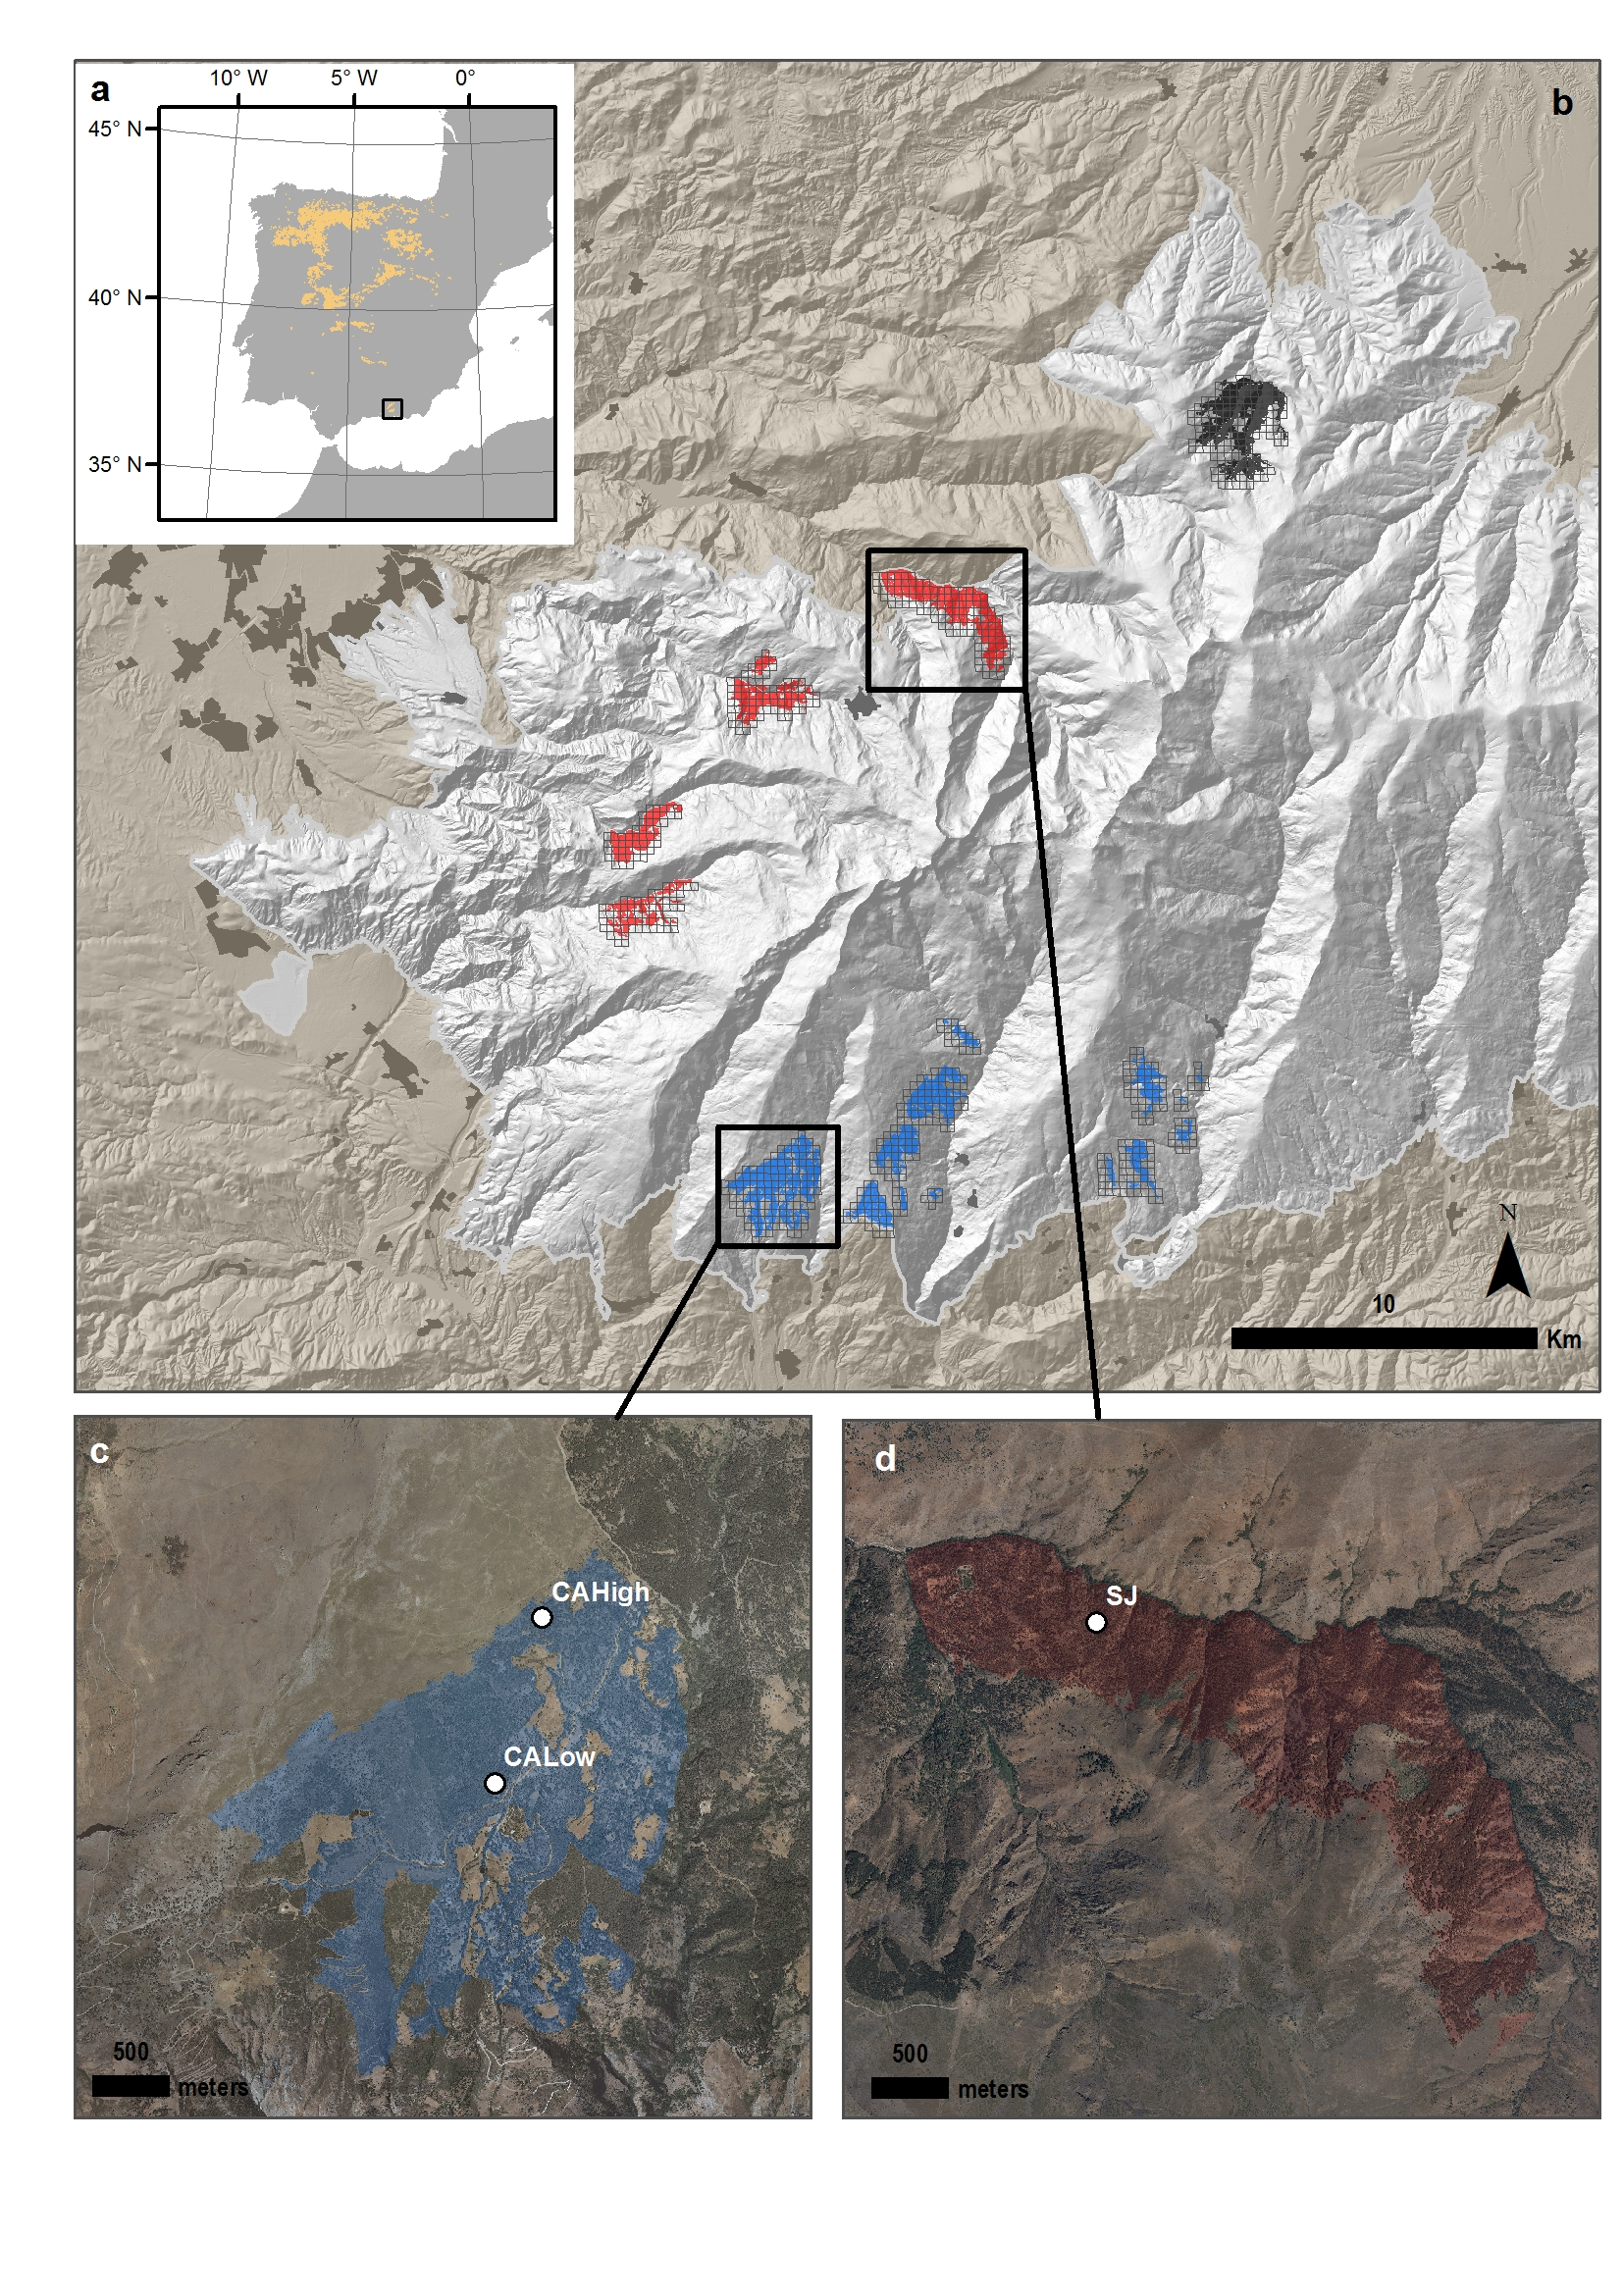
\includegraphics[width=\textwidth]{img/dendro/dendro-mapa.jpg} \caption{Distribution of \textit{Quercus pyrenaica} forests in the Iberian Peninsula \textbf{a} and in Sierra Nevada mountain range \textbf{b}. Different colors indicate oak-population clusters identified in Sierra Nevada \autocite{PerezLuque2015}. For each population, a grid with the MODIS pixels is shown (see Material and methods). Detailed location of the dendroecological sampling sites: northern (San Juan, SJ) \textbf{c}, and southern ones (Cáñar: CA-Low and CA-High) \textbf{d}. Color orthophotography of 2009 from Regional Ministry of the Environment.}
\label{fig:dendro:map}
\end{figure}

The forests of this species reach their southernmost European limit in Andalusian mountains such as Sierra Nevada (37°N, 3°W), a high-mountain range with elevations of up to 3482 m \emph{a.s.l.}. The climate is Mediterranean, characterized by cold winters and hot summers, with pronounced summer drought and increasing aridity with decreasing altitude, and marked variability in annual rainfall according to elevation and aspect. Sierra Nevada is considered a glacial refuge for deciduous \emph{Quercus} species \autocite{Olaldeetal2002WhiteOaks}. Eight Pyrenean oak patches (2400 ha) have been identified in this mountain range (\figref{fig:dendro:map}), from 1100 to 2000 m \emph{a.s.l.} and often associated with major river valleys. Today, \Qpy woodlands in this mountain region represent a rear edge of their habitat distribution \autocite{HampePetit2005ConservingBiodiversity}. They are the richest forest formation in vascular plant species of Sierra Nevada, containing several endemic and endangered plant species \autocite{Loriteetal2008PhytosociologicalReview}. They also harbor high levels of intraspecific genetic diversity \autocite{ValbuenaCarabanaGil2013GeneticResilience}. These relict forests have undergone intensive human use throughout history \autocite{CamachoOlmedoetal2002DinamicaEvolutiva}. Furthermore, the conservation status of this species for southern Spain is considered ``Vulnerable'' and it is expected to suffer from climate change, potentially reducing its suitable habitats in the near future \autocite{GeaIzquierdoetal2013GrowthProjections,GeaIzquierdoetal2017RiskyFuture}.

\subsection{Climatic data and drought episodes}\label{sec:dendro:Climate}
The Iberian Peninsula underwent several extreme drought episodes in the last three decades \autocite[\emph{e.g.} 1995, 1999, 2005, 2012][]{VicenteSerranoetal2014EvidenceIncreasing}. The 2005 and 2012 drought events have been documented as being among the worst in recent decades for the southern Iberian Peninsula \autocite{Pascoaetal2017DroughtTrends}, appearing as extreme drought in our climatic data (\figref{fig:dendro:s1climate}; \tabref{tab:dendro:droughts}). We focused on these two drought events because they were included in the period having remote-sensing information of high spatial resolution (MODIS started on 2000; see below). Nevertheless, for radial growth-time series, a greater number of older drought events were also analyzed to contextualize the results for 2005 and 2012 and to evaluate forest resilience to drought over a longer term (see \tabref{tab:dendro:droughts}). A drought event was identified using the SPEI (Standardized Precipitation-Evapotranspiration Index) \autocite{VicenteSerranoetal2010MultiscalarDrought} (SPEI 12-months scale), following a procedure similar to the one proposed by \textcite{Spinonietal2015EuropeanDrought}. We used 0.5º grid cells covering Sierra Nevada taken from the Global SPEI Database (\url{http://spei.csic.es/database.html}). A severe drought event starts when SPEI falls below the threshold of -1.28 \autocite{Spinonietal2018WillDrought,Pascoaetal2017DroughtTrends}. A drought event is considered only when SPEI values fall below that threshold for at least two consecutive months. For each drought event, we computed: the \emph{duration} as the number of consecutive months with the SPEI lower than a certain threshold; the \emph{severity} as the sum of the absolute SPEI values during the drought event; the \emph{intensity} and the \emph{Lowest SPEI} refer to the mean and lowest value of SPEI respectively during the drought event.

To explore the relationships between climatic variables and tree-growth variables we used climate data obtained from the European Daily High-Resolution Observational Gridded Dataset (E-OBS v16) \autocite{Haylocketal2008EuropeanDaily}. Monthly precipitation and minimum and maximum temperatures had a 0.25 x 0.25 º resolution for the 1950-2016 period. Grid cells were selected to cover each sampled site. The SPEI 6-months scale index was used to characterize the drought conditions for the period 1961-2014.

\subsection{Greenness data to assess ecosystem resilience}\label{sec:dendroEVI}
Vegetation greenness of \Qpy was characterized by means of the \emph{Enhanced Vegetation Index} (EVI), derived from MOD13Q1 product of the MODIS sensor. EVI data consists of 16-day maximum value composite images (23 per year) of the EVI value with a spatial resolution of 250 m x 250 m. MODIS EVI data were compiled for the period 2000 - 2016. We selected the pixels covering the distribution of \Qpy forests in Sierra Nevada (\emph{n} = 928 pixels). Any values affected by clouds, snow, shadows or high content aerosols, were filtered out following recommendations for mountain regions \autocite{ReyesDiezetal2015ImplicacionesFiltrado}.

The mean Annual EVI (\(EVI_{mean}\)) as a surrogate of mean annual primary production was computed for each pixel for the period 2000 - 2016. The EVI standardized anomaly (\(EVI_{sa}\)) was computed pixel-by-pixel, in order to minimize bias in the evaluation of anomalies and to provide more information concerning their magnitude \autocite{Samantaetal2012InterpretationVariations}. For each pixel, an annual EVI value was calculated by averaging EVI valid values. Then, the standardized anomaly was computed as: \[\mathrm{EVI_{sa,\mathit{i}}}= (\mathrm{EVI_{mean,\mathit{i}}-EVI_{mean,ref}})\Big/\sigma_{\mathrm{ref}}\]
where \(\mathrm{EVI_{sa,\mathit{i}}}\) is the EVI standardized anomaly for year \(i\); \(\mathrm{EVI_{mean,\mathit{i}}}\) the annual mean value of EVI for year \(i\); \(\mathrm{EVI_{mean,ref}}\) the average of the annual EVI values for the period of reference 2000-2016 (all except year \(i\)); and \(\sigma_{\mathrm{ref}}\) the standard deviation for the reference period. Each pixel was categorized according the EVI standardized anomalies as ``greening'' (\(EVI_{sa} > 1\)), ``browning'' (\(EVI_{sa} <- 1\)) or ``no-changes'' (\(-1 > EVI_{sa} > 1\))\autocite{Samantaetal2012InterpretationVariations}.

Rather than other vegetation indices such as the NDVI, \(EVI_{mean}\) was chosen because it is highly stable under the use of any filter \autocite{ReyesDiezetal2015ImplicacionesFiltrado} and because it showed highly significant correlations with annual (\(r\)= 0.81) and seasonal EVI values (\(r_{spring}\)= 0.76 and \(r_{summer}\)= 0.88).

\subsection{Field sampling and dendroecological methods to assess individual tree resilience}\label{sec:dendro:Field}
Trees were sampled during the autumn of 2016 at two locations in contrasting N-S slopes of Sierra Nevada: San Juan (SJ), a xeric site located at the northern aspect (around 1400 m); and Cáñar (CA), a wetter site located at the southern aspect (\figref{fig:dendro:map}; \tabref{tab:dendro:sampledPlots}). For the southern site, two elevations were sampled: CA-Low (around 1700 m) and CA-High (around 1860 m), constituting the current low-elevational limit for the species (CA-Low) and the maximum altitude currently reached by trees (CA-High), respectively, in the site sampled. Despite the proximity of these two elevations (less than a 200-m difference) the stands differ markedly in their structure and characteristics (\tabref{tab:dendro:sampledPlots}). The three sampling sites followed a moisture gradient: SJ \textless{} CA-Low \textless{} Ca-High (\tabref{tab:dendro:sampledPlots}). All the sites were oak monospecific and representative of the population clusters identified for the species in this mountain range \autocite{PerezLuqueetal2015DatasetMIGRAME}. At each site, between 15 and 20 trees from either the single dominant-codominant layer in CA or the open canopy in SJ were randomly sampled. Two cores of 5 mm in diameter were taken from each tree at breast height (1.3 m) using an increment borer. Diameter at breast height (DBH) and total height were measured for each tree. In addition, stand competition affecting target trees was assessed by recording distance, azimuth, DBH, species, and total height of all neighboring living trees with DBH \textgreater{} 7.5 cm within a circular plot with a 10-m radius. Several competition indices were calculated: the distance independent indices \emph{density} (\(\mathrm{trees \cdot ha^{-1}}\)), and \emph{basal area} (BA, \(\mathrm{m^{2} \cdot ha^{-1}}\)); and the distance dependent index size ratio proportional to distance \autocite[see][ for more details]{GeaIzquierdoCanellas2009AnalysisHolm} as: \[\mathrm{srd} = \sum_{i=1}^{n} (dbh_j / dbh_i) \cdot \left[1/ (dist_{ij} + 1) \right ]\]

Tree cores were air dried, glued onto wooden mounts, and sanded. Annual radial growth (ring width, RW) was determined with a measuring device coupled to a stereomicroscope, for an accuracy of 0.001 mm. Individual ring series were first visually and statistically cross-dated with TSAP software (Rinntech, Heidelberg, Germany), using the statistics Gleichläufigkeit (GLK), t-value and the crossdating index (CDI). Cross-dating validation was finally verified using COFECHA \autocite{Holmes1983ComputerassistedQuality}.

The growth trends were analyzed at different time scales. To study the growth response to the inter-annual variability of climate (short-term response), pre-whitened residual chronologies (RWI) were used. These were calculated from ratios between raw growth measurements and individual cubic splines with a 50\% frequency cutoff at 30 years \autocite{Fritts1976TreeRings}. Tree-ring width series were standardized and detrended using dplR \autocite{Bunn2010StatisticalVisual}. Mean residual site chronologies were established by computing the biweight robust mean of all prewhitened growth indices for the trees of the same site \autocite{Fritts1976TreeRings}. The statistical quality of each chronology was checked via the expressed population signal (EPS). A threshold value of EPS \textgreater{} 0.85 was used to determine the cutoff year of the time span that could be considered reliable.

The long-term growth response was analyzed using basal area increment (hereafter BAI, \(\mathrm{cm^2 \cdot year^{-1}}\)). In theory, BAI represents a more accurate indicator of growth than ring width, because it removes variation in growth attributable to increasing stem circumference after 30-40 years of juvenile growth \autocite{BiondiQeadan2008TheorydrivenApproach}. Raw ring widths and measured DBH were used to compute BAI \autocite{Piovesanetal2008DroughtdrivenGrowth} with the following equation: \[\mathrm{BAI} = \pi(r^2_{t}-r^2_{t-1})\] where \(r\) is the radius of the tree and \(t\) is the year of tree-ring formation. For each individual tree, a mean BAI series was calculated. Then, mean site BAI chronologies were determined by averaging individual tree BAI time series.

\subsection{Disturbance analyses and land-use history review}\label{sec:dendro:Disurbance}
Disturbance chronologies were built using tree-ring width to identify abrupt and sustained increases (release events from competition) or decreases (suppressions) in radial growth \autocite{NowackiAbrams1997RadialgrowthAveraging} as indirect estimates of possible disturbance events (\emph{e.g.} logging, drought-induced neighbor mortality) in the past. Growth changes (GC) were calculated for the individual tree-ring series using a 10-year running window as either positive (PGC) or negative (NGC) growth changes: \[\mathrm{\% GC} = \left[(M1 - M2)\Big/ M2\right] \times 100\] where \(M1\) is the preceding 10-year median and \(M2\) is the subsequent 10-year median \autocite{RubinoMcCarthy2004ComparativeAnalysis}.

Site-disturbance chronologies were constructed by annually averaging the individual disturbance series. To separate growth peaks caused by disturbance events and expressing stand-wise disturbances from those caused by climate, we considered a threshold of 50\% of GC and more than 50\% of the individual trees displaying the same growth changes \autocite[\emph{e.g.}][]{GeaIzquierdoCanellas2014LocalClimate}. In addition, the history of the forest and management of our sampling sites was inferred from a detailed analysis of historical land-use changes. For this, existing historical documents were exhaustively reviewed to compile information on socio-economical activities affecting the forests being studied (\tabref{tab:dendro:reviewusos}). We exhaustively reviewed existing documentary sources: historical documents and maps; detailed mining reports; official information on recent wildfires events and forest-management practices; livestock farming; traditional irrigation channels; and studies concerning the socioeconomic dynamics of forests on Sierra Nevada at different spatio-temporal scales (see \tabref{tab:dendro:reviewusos} for references).

\subsection{Assessing resilience to drought at the forest stand and individual-tree levels}\label{sec:dendro:Resilience}
To evaluate the effects of drought events on ecosystem resilience (using greenness data) and individual tree resilience (using BAI data), we used resilience indices proposed by \textcite{Lloretetal2011ComponentsTree}. The Resistance index estimated as the ratio between performance during and before the disturbance (\(Resistance=Drought/PreDrought\)) quantifies the severity of the impact of the disturbance in the year it occurred. The Recovery index, computed as the ratio between performance after and during disturbance (\(Recovery= PostDrought/Drought\)), represents the ability to recover from disturbance relative to its severity. Finally, the Resilience index (\(Resilience = PostDrought/PreDrought\)) is the capacity to reach pre-disturbance performance levels. The values of these indices were computed for tree growth (BAI) and greenness (EVI mean) during each drought event. The predrought and postdrought values of each target variable (\emph{i.e.} BAI or EVI) were computed as the mean value over a period of three years before and after the drought event, respectively. A period of three years was chosen because we found similar results on comparing periods of two, three, and four years (\figref{fig:dendro:s3correlations}b), and this time period has been used in other studies \autocite[\emph{e.g.}][]{Gazoletal2018ForestResilience}. Resilience metrics for BAI data were additionally computed for the most severe drought events since 1940 (\emph{n} = 8; \tabref{tab:dendro:droughts}) and compared with drought severity.

\begin{figure}
\centering
\includegraphics[width=\textwidth]{img/dendro/dendro-schema.jpg} \caption{Schema of the different metrics \textbf{a} and analyses \textbf{b} used in the manuscript (see Material and methods for details). The severe drought events since 1901 were identified using SPEI-12 and characterized in terms of duration, severity and intensity. Climate impacts on vegetation were assessed for greenness and tree-growth. Non climatic disturbances on vegetation were quantified using growth changes on tree growth (\%GC) and were also related with anthropogenic alterations inferred from review of historical documents. Responses of vegetation to disturbances were explored in the short- and the long-term using resilience metrics and temporal trends respectively for both EVI and BAI. Resilience metrics of BAI were computed for the eight most severe drought events since 1950, and their relationship with drought severity were explored. For the 2005 and 2012 drought events we also compared EVI and BAI resilience metrics among the three \textit{Q. pyrenaica} populations. Numbers (\textit{grey circles}) indicate the study aims to which the analyses are related.}
\label{fig:dendro:schemadendro}
\end{figure}

\begin{table}
\caption{Characteristics of the mean tree-ring chronologies. Length values in parentheses indicate the number of years replicated with more than five series. \emph{RW} = mean annual ring width (standard deviation in parenthesis). MS = mean sensitivity. AR(1) = mean autocorrelation of raw series. Rbt = mean correlation between series. EPS = mean expressed population signal. EPS and Rbt were calculated for the mean residual chronologies of growth indices.}
\resizebox{\linewidth}{!}{
\begin{tabular}{@{}lllllllllll@{}}
\toprule
Site & First year & Last year & Length (years) & \#    trees & \#    cores & RW (mm) & MS & AR(1) & Rbt & EPS \\ \midrule
CA-Low & 1836 & 2016 & 181 (164) & 15 & 30 & 1.253 (0.781) & 0.208 & 0.799 & 0.520 & 0.897 \\
CA-High & 1819 & 2016 & 198 (188) & 15 & 30 & 1.500 (0.879) & 0.203 & 0.827 & 0.522 & 0.907 \\
SJ & 1921 & 2016 & 96 (90) & 20 & 48 & 1.725 (1.207) & 0.319 & 0.692 & 0.637 & 0.959 \\ \bottomrule
\end{tabular}}
\label{tab:dendro:chronologies}
\end{table}

\subsection{Statistical analysis}\label{sec:dendro:Stats}
Differences between sites for height, DBH, and competition indices were analyzed using non-parametric Kruskal-Wallis rank sum tests. When significant differences were detected, multiple comparisons were run using the Dunn test with Bonferroni adjustment to correct for significance.

The severe drought events since 1901 were identified using SPEI-12. They were characterized in terms of duration, severity and intensity \autocite[see][]{Spinonietal2015EuropeanDrought}. In a first step, the impact of drought in greenness and growth was explored using the \(EVI_{sa}\) and the mean RWI site chronologies (\figref{fig:dendro:schemadendro}). Additionally the relationships between climatic variables and tree-growth variables (RWI and BAI site chronologies) were assessed using bootstrapped Pearson's correlations estimated using treeclim \autocite{ZangBiondi2015TreeclimPackage}. The non-climatic disturbance impacts on tree-growth were evaluated using site disturbance chronologies (built using growth changes on tree growth).

Responses of vegetation to disturbances were explored in the short- and the long-term using resilience metrics (resilience, resistance and recovery) and temporal trends respectively for both EVI and BAI (\figref{fig:dendro:schemadendro}). Resilience metrics of BAI were computed for the eight most severe drought events since 1950 (including 2005 and 2012), and their relationship with drought severity were explored. Resilience metrics of EVI were computed only for 2005 and 2012 drought events. Temporal trends of \(EVI_{mean}\) (pixel scale) and BAI (mean BAI site chronologies) were examined using non-parametric (Mann-Kendall) and parametric test (Pearson) respectively.

\begin{figure}
\centering
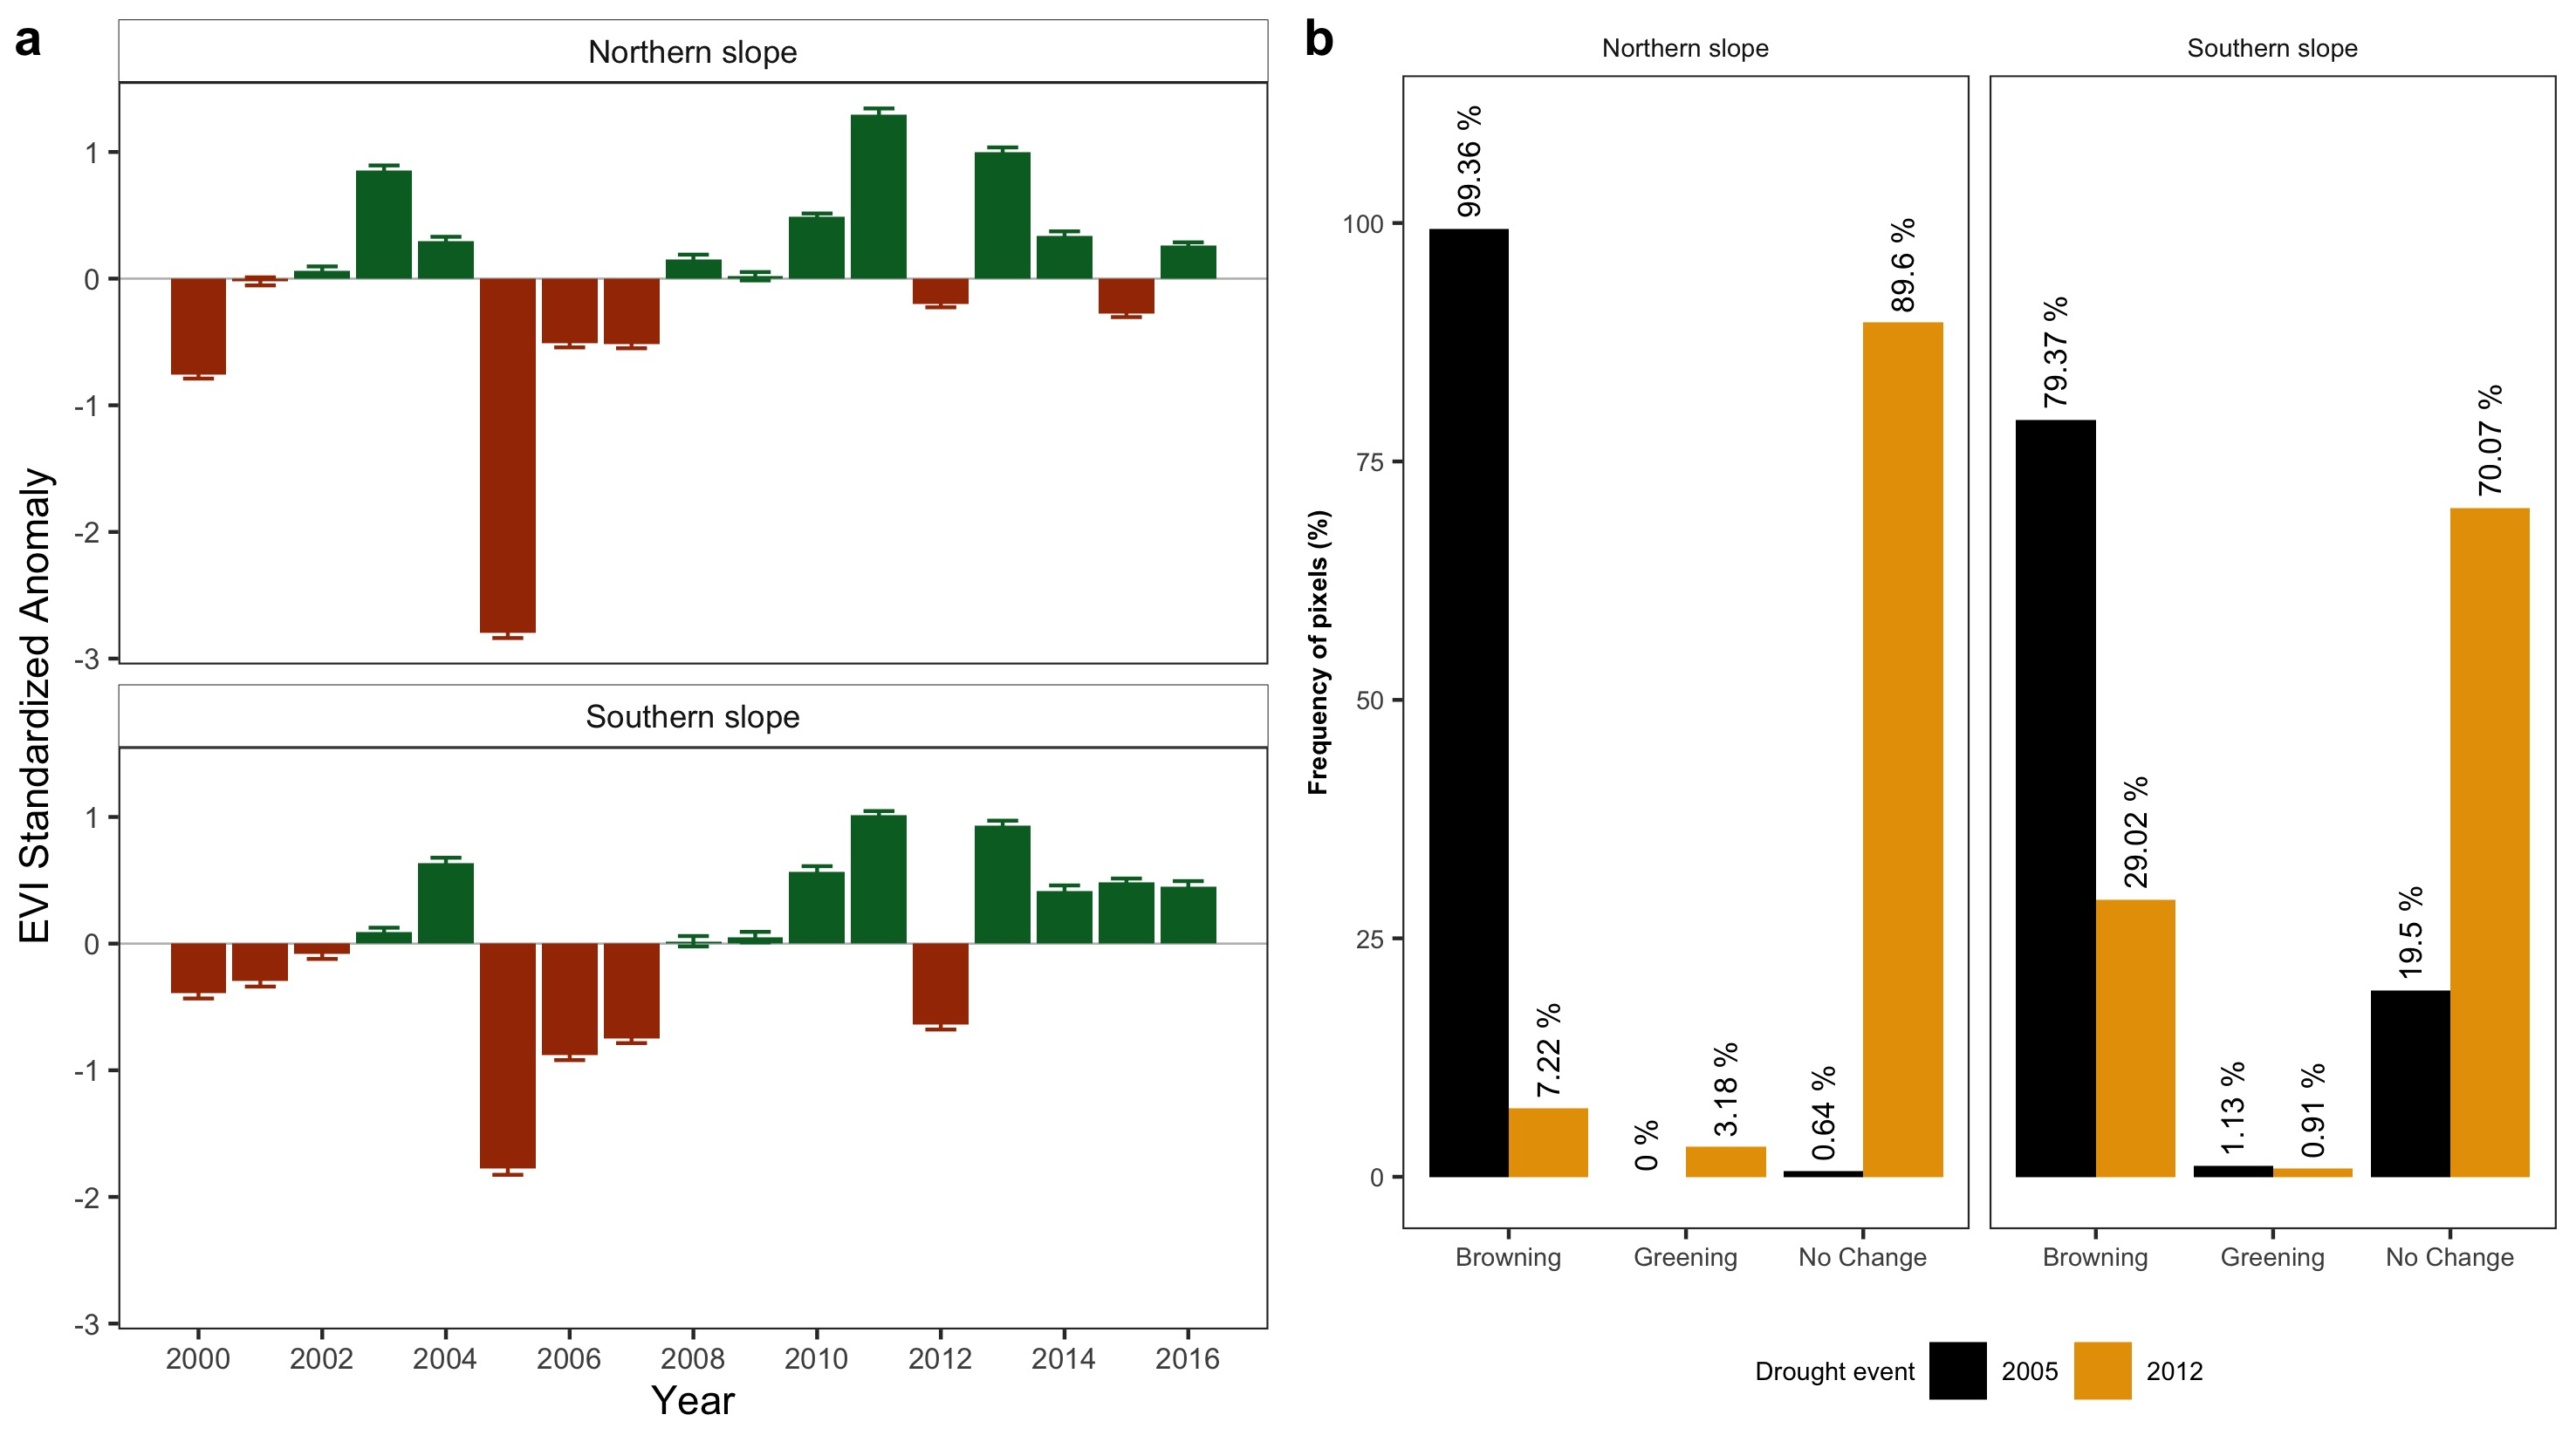
\includegraphics[width=\textwidth]{img/dendro/dendro-evisa.jpg} \caption{EVI standardized anomaly during the period 2000-2016 for northern and southern populations \textbf{a}. Error bars show standard error. See main text for details on EVI calculation. Percentage of pixels showing browning, greening or no changes during the 2005 and 2012 drought events according to EVI standardized anomalies \textbf{b}. See main text for an explanation of greening and browning.}
\label{fig:dendro:evisa}
\end{figure}

For each of the three resilience indices studied, we used robust two-way ANOVAs to test for differences between drought events (2005 and 2012) and the oak populations studied (northern and southern exposures). These tests were used because original and log-transformed data did not follow the assumptions of normality or homogeneity of variance \autocite{Wilcox2012IntroductionRobust}. Robust measures of central tendency (M-estimator based on Huber's Psi) were used because they were close to the mean value in all cases \autocite{Wilcox2012IntroductionRobust}. When the robust ANOVA test was run, data were bootstrapped 3000 times and trimmed automatically to control the potential influence of outliers. \emph{Post-hoc} differences were assessed pairwise using a similar bootstrap test. All the robust ANOVA and \emph{post-hoc} tests were carried out using the WRS2 R package \autocite{Mairetal2017WRS2Wilcox}. The level of significance was set to 0.05 and adjusted for multiple comparisons.

\section{Results}\label{sec:dendro:Results}
\subsection{Temporal trends in vegetation greenness}\label{sec:dendro:ResultsEVI}

The analysis of temporal trends in greenness showed that 78.9\% of the EVI pixels followed a positive trend for the 2000-2016 period. The lowest values of EVI standardized anomalies for the study period were recorded during the 2005 drought, and the minimum EVI values were expressed in the northern (dry) population (\figref{fig:dendro:evisa}a). A ``browning'' episode (\(\mathrm{EVI_{sa}} < -1\)) was found during this drought event, whereas no changes in greenness in response to the 2012 drought were detected (\figref{fig:dendro:evisa}b).

\subsection{Analysis of radial-growth trends and disturbances}\label{sec:dendro:ResultsBAI}
The trees of the southern population were older than those from the northern one (\tabref{tab:dendro:chronologies}). In addition, trees from the southern population at high elevation were taller and their growth was significantly greater than that of trees from the other two sites. Stand competition measured as plot basal area was greatest in CA-High (\tabref{tab:dendro:sampledPlots}, \figref{fig:dendro:bai}a). The growth and height of trees from the northern and the low-elevation southern population were similar (\figref{fig:dendro:bai}a and \figref{fig:dendro:s3correlations}a). Only trees from the southern sites (\emph{i.e.} the wetter exposure) showed significant positive growth trends since the late 1970s (\figref{fig:dendro:bai}a), this trend being far more pronounced for the wetter and colder high elevation site (CA-High).

Drought events reduced radial growth for all sites (\figref{fig:dendro:s2chronos}a). The strongest reduction in radial growth occurred in response to the 1995 drought (the worst drought spell in our climatic record, \tabref{tab:dendro:droughts}) for all sites. Tree-growth reductions in response to drought followed a moisture gradient. Tree-growth reductions in response to the studied drought events were lower in the southern sites (CA-High and CA-Low) than in the northern site (SJ), especially for 2005 and 2012 (\figref{fig:dendro:s2chronos}a). The weakest growth reductions were found in trees from the wettest site (CA-High).

The response of tree growth to water availability was greater than to temperatures. Cumulative precipitation of the hydrological year and seasonal SPEI values (\emph{i.e.} for the Hydrological year, Spring and Summer) were the climatic variables exhibiting the highest (positive) relationship with growth for all populations (\figref{fig:dendro:s6corclimate}a). Nevertheless, there were differences between populations: the positive relationship with SPEI was highest in the more xeric northern population (r \textgreater{} 0.6 \emph{vs.} r \textless{} 0.5; \figref{fig:dendro:s6corclimate}a).

The northern site (SJ) showed two major release events (GC \textgreater{} 50\% occurring in more than 50\% of trees sampled): the first during the 1940s (the most evident) and the second in 1995-2000 (\figref{fig:dendro:bai}b). These periods alternated with periods of suppression. By contrast, the two southern sites showed no release events except for CA-High at the beginning of the 1830s and no suppression events in the last 50 years.

\begin{figure}
\centering
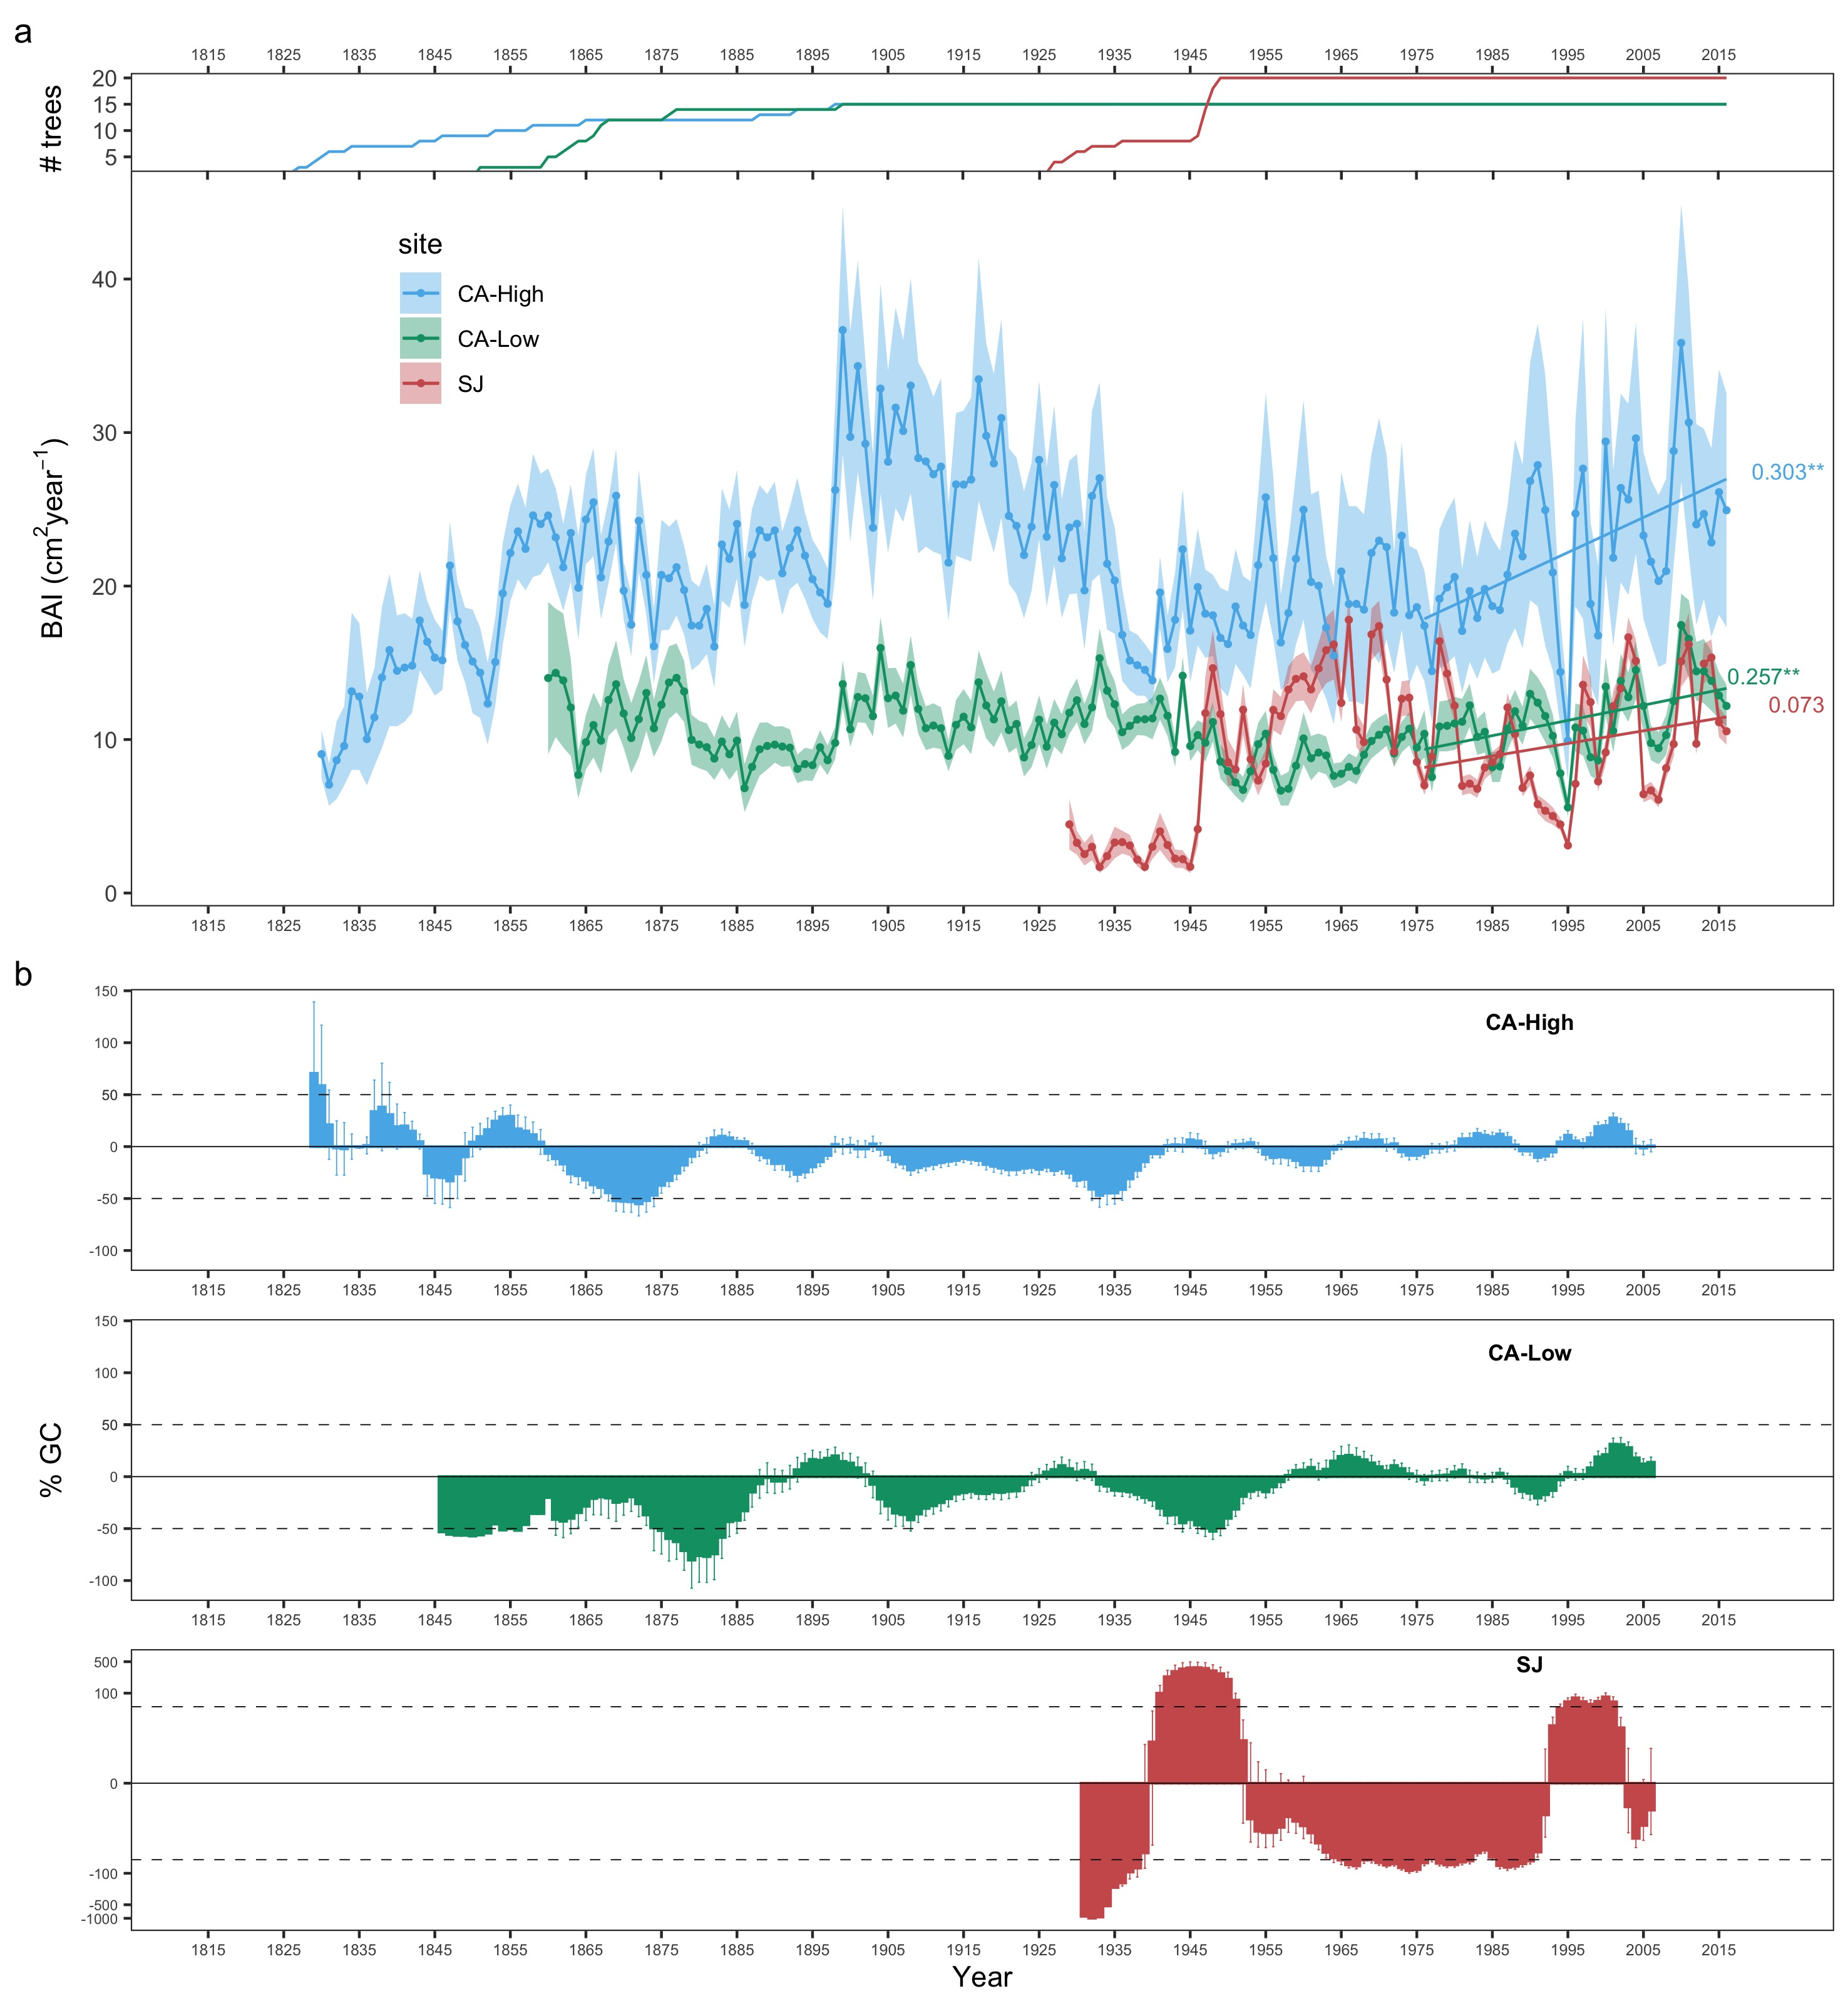
\includegraphics[width=\textwidth]{img/dendro/dendro-cronos-bai-gc.jpg}\caption{
Basal Area Increment (BAI) chronologies of \textit{Q. pyrenaica} for northern population (SJ; \textit{red}) and southern ones: low-elevation (CA-Low; \textit{green}) and high-elevation (CA-High, \textit{blue}) sites \textbf{a}. Shading areas correspond to standard error of the mean. Number of series is displayed in the upper plot. Only years replicated with \# series \textgreater{} 5 are shown. Linear trends since 1975 are indicated for all sites (numbers indicate \(r^2\) values; asterisks indicate significant linear trend, p \textless{} 0.001). Comparison of median growth change (\(GC\)) following \textcite{NowackiAbrams1997RadialgrowthAveraging} for \textit{Q. pyrenaica} sites \textbf{b}. Dashed black lines indicate a threshold of 50\% of GC (see Material and methods). Note that y-axes do not correspond in all of the three panels for the sake of clarity. Error bars indicate standard error.}
\label{fig:dendro:bai}
\end{figure}

\subsection{Resilience, resistance and recovery to drought events at the stand and individual-tree levels}\label{sec:dendro:ResultsResilience}

Resilience and resistance varied in the same direction whereas recovery varied inversely to resilience and resistance. During the last two drought events, resilience metrics for greenness and tree growth significantly differed between drought events (\tabref{tab:dendro:robustanova}). The 2005 drought event reduced greenness and growth more than that of 2012 (\tabref{tab:dendro:huber}) but the metrics of resilience generally covaried in the same direction during those two drought events. For EVI, resilience and resistance values were significantly higher for 2012, the most severe event, than for 2005 (\tabref{tab:dendro:huber}; \figref{fig:dendro:resilience}b); whereas recovery values were higher for 2005 than for the 2012 drought event. For BAI, the resilience, resistance and recovery values were higher for 2012 than for 2005 (\tabref{tab:dendro:huber}, \figref{fig:dendro:resilience}c).

The recovery and resistance for greenness and growth varied significantly between sites. Resilience calculated for greenness also differed between sites but not for tree growth (p = 0.534; \tabref{tab:dendro:robustanova}). The two southern populations showed lower recovery values than did the northern site both for greenness and tree growth, but resistance and resilience values were significantly higher for the southern site (\tabref{tab:dendro:huber}).

Resilience metrics of tree-growth for drought events since 1950 (\emph{i.e.} shared period among the three chronologies excluding the juvenile years, \tabref{tab:dendro:droughts}) revealed a positive relationship between drought severity and recovery, significant for all oak populations (\figref{fig:dendro:resilience}a). A similar pattern was found for resilience but proved significant only for SJ. Importantly, non-significant patterns resulted when we excluded 1995, except for recovery in SJ (\figref{fig:dendro:s5resilience}). The trees showed the highest value of tree-growth resilience for 1995, the worst drought event in our study area, particularly SJ where our results suggest a major release event also after 1995 (\figref{fig:dendro:bai}b).

\section{Discussion}\label{sec:dendro:Discussion}
By using a combined approach of remote-sensing information and dendroecology, we quantified the growth of adult trees and greenness (EVI) as proxies for secondary and primary growth of relict Mediterranean \Qpy populations in the southern Iberian Peninsula. These relict oak populations, driven by historical land-use, have been resilient to climate change at their present rear edge. However, resistance, resilience, and forest recovery after extreme drought events were strongly influenced by mountain exposure, local environmental conditions, and management legacies. This means that the geographical and the ecological rear edges do not necessarily match and, at a small spatial scale, tree performance can vary markedly along the rear edge under climate change.

\begin{figure}
\centering
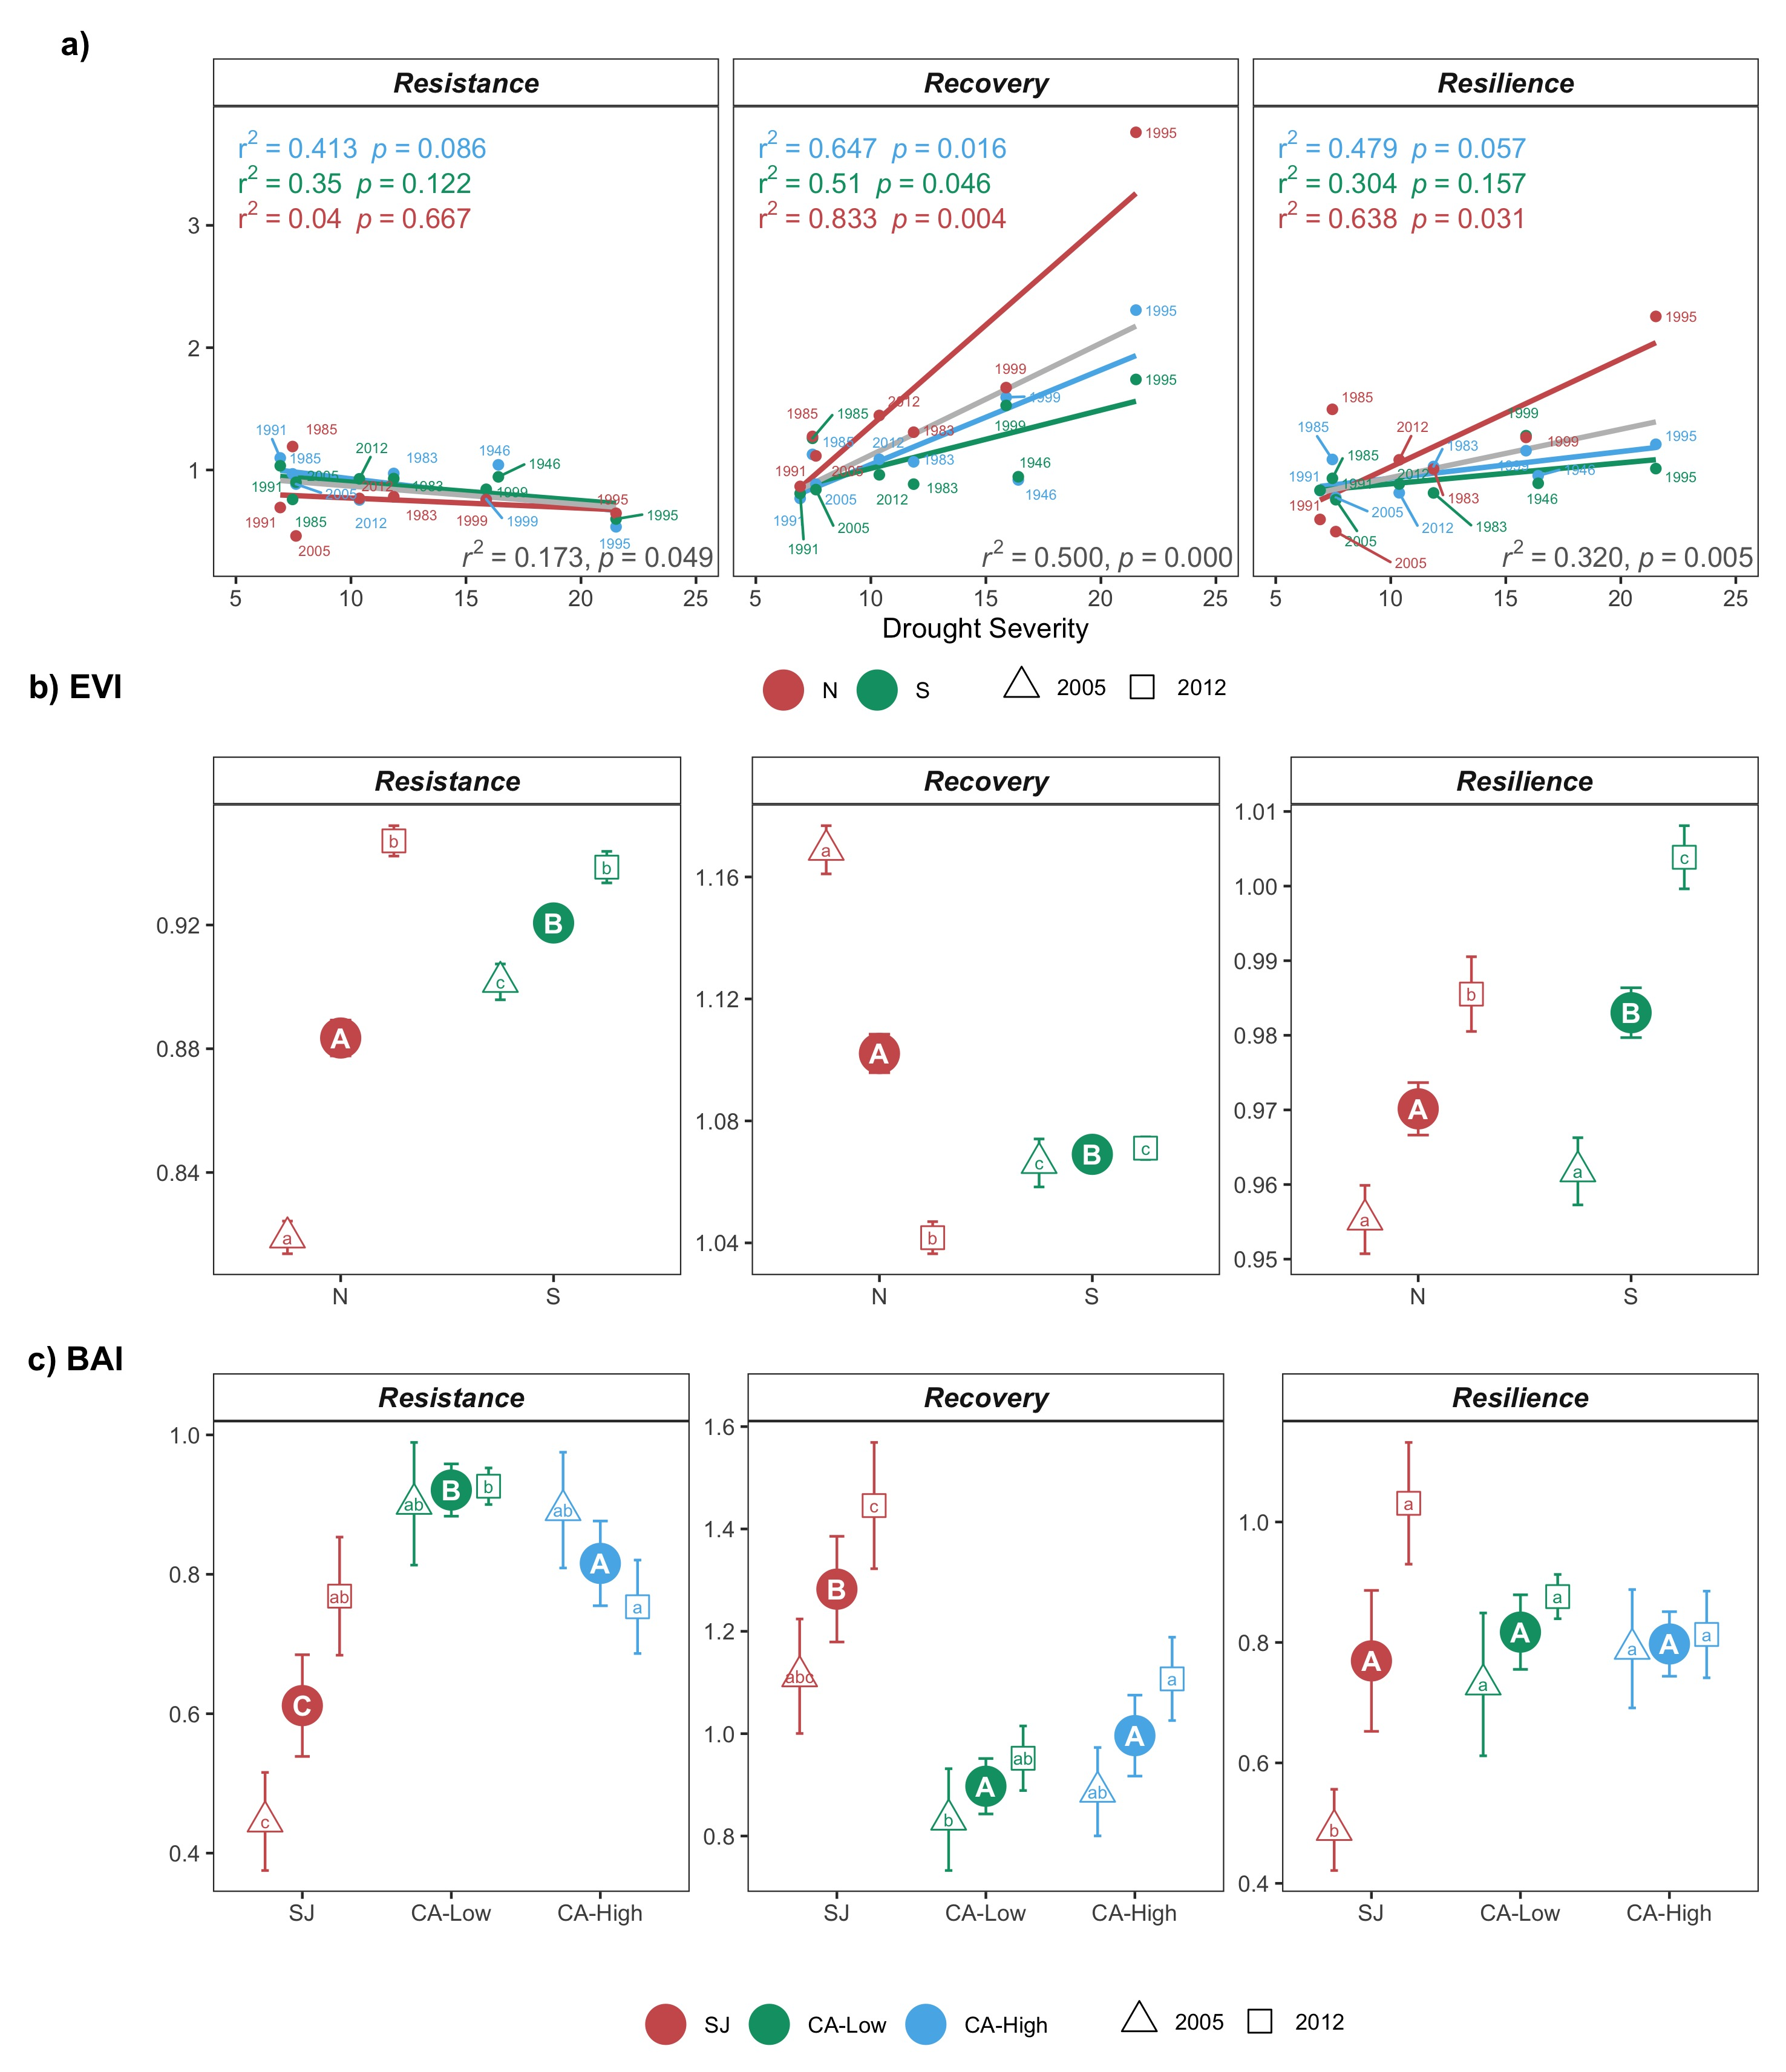
\includegraphics[width=\textwidth]{img/dendro/dendro-resiliences.jpg}\caption{
Resilience metrics of tree-growth for eight severe drought events since 1950 (see main text for details) as a function of drought severity \textbf{a}. Points indicate resilience metrics for oak populations: SJ (\textit{red}), CA-High (\textit{blue}) and CA-Low (\textit{green}). Resilience metrics were computed for each population (sample depth > 10) and drought event. Gray lines represent overall relationships for each Resilience metrics. Comparison of the response of  *Q. pyrenaica* forests to drought in terms of resistance, recovery, and resilience of greenness (\textbf{a}) and tree growth (\textbf{c}). For EVI, northern populations (\textit{red circle}) were compared with southern ones (\textit{green circle}). For BAI, the more xeric northern population (San Juan, SJ; \textit{red circle}) was compared with the two southern populations, Cáñar-High (CA-High; \textit{blue circle}) and Cáñar-Low (CA-Low; \textit{green circle}). Different letters indicate significant \textit{post hoc} differences between groups (see Material and methods for details).} 
\label{fig:dendro:resilience}
\end{figure}
\hypertarget{sec:dendroHighSensitivity}{%
\subsection{High sensitivity and variability in the oak sensitivity to climate at the rear edge}\label{sec:dendroHighSensitivity}}

Severe drought negatively affects both primary and secondary growth of \Qp forests. This was expressed by the observed reduction in greenness and tree growth in response to the 2005 and 2012 drought events as well as by radial-growth suppression during extreme drought events \autocite{Corcueraetal2006RadialgrowthWoodanatomical,GeaIzquierdoCanellas2014LocalClimate}. Furthermore, the greatest reduction of tree growth was detected during the 1995 drought, a characteristic negative precipitation anomaly that caused severe and extensive damage in the Mediterranean Iberian Peninsula \autocite{Penuelasetal2001SevereDrought,Gazoletal2018ForestResilience}.

The tree responses to drought are site-dependent \autocite{Babstetal2013SiteSpecies}, particularly for rear-edge populations \autocite{CavinJump2017HighestDrought,DoradoLinanetal2017LargescaleAtmospheric}. Greenness and tree growth were more affected by drought events in drier northern populations than in wetter southern oak populations of Sierra Nevada. The northern site showed higher browning intensity than did the southern sites during the 2005 drought event, and stronger correlations of tree-growth with SPEI (hydrological year and summer) at the northern site can be interpreted as higher sensitivity to drought at drier sites \autocite{GeaIzquierdoCanellas2014LocalClimate}. Greenness was less sensitive to drought than tree growth, particularly for drier sites. These findings agree with previous works showing tree growth to be a more sensitive metric of forest resilience than is net primary productivity \autocites[\emph{e.g.}][]{Babstetal2013SiteSpecies,Coulthardetal2017TreeGrowth,Gazoletal2018ForestResilience,PenaGallardoetal2018DroughtSensitiveness}, suggesting that the growth reduction could be mediated by sink more than by source limitations \autocite{Korner2013GrowthControls,Fatichietal2014MovingPhotosynthesis}. On the other hand, trees at CA-High registered higher BAI than did those located at lower elevations (CA-Low and SJ; \figref{fig:dendro:bai}). This shows the high variability in the response to climate exhibited along a narrow gradient, which was especially noteworthy for southern sites, as these lie close to each other and both are considered to constitute the rear edge for the species.

As with many other forest species under Mediterranean climates, moisture availability is generally the most limiting factor driving radial growth of \Qp along its distribution range in the Iberian Peninsula \autocite{GeaIzquierdoCanellas2014LocalClimate}. Thus, our results are consistent with those of previous studies highlighting the influence of precipitation on tree-ring growth in different oak species \autocites[\emph{e.g.}][]{Tessieretal1994DeciduousQuercus,DiFilippoetal2010ClimateChange,GeaIzquierdoetal2011TreeringsReflect,GarciaGonzalezSoutoHerrero2017EarlywoodVessel}. A positive effect of moisture availability and negative impact of temperature expressing a limiting effect of high vapor-pressure deficit and potential evapotranspiration can be expected at drought-limited rear-edges. Yet, at the rear edge, the growth of some tree species (\emph{e.g.} \emph{Abies alba}) has been shown to be more sensitive to moisture-related variables \autocite{MartinezSanchoGutierrezMerino2019EvidenceThat}, while others species were more sensitive to temperatures \autocite[\emph{e.g.} \emph{Pinus sylvestris},][]{Herreroetal2013VaryingClimate}, and still other species responded simultaneously to both temperature and moisture-related variables \autocites[\emph{e.g.} \emph{Fagus sylvatica},][]{DoradoLinanetal2017CoexistenceMediterraneanTemperate,DoradoLinanetal2017ClimateThreats}[\emph{Pinus nigra} subsp. \emph{salzmanii},][]{SanchezSalgueroetal2012DroughtMain}. This diversity in the response of tree species to precipitation and temperature suggests that vulnerability to climate change is not consistently expressed within the rear edge, therefore evidencing that geographically marginal forests are not necessarily climatically or ecologically marginal \autocite[see][ and references therein]{DoradoLinanetal2019GeographicalAdaptation}.

\subsection{Relict oaks show high resilience to drought at different spatio-temporal scales: do the geographical and ecological rear-edges match?}\label{sec:dendro:Relict}
Despite the severe drought events in recent decades (\tabref{tab:dendro:droughts}), we found a positive trend for vegetation greenness of \Qp for the last 16 years. This is consistent with previous findings stressing a recent short-term increase in primary productivity for these forests coinciding with a rather wet decade in the 2000s after a dry decade in the 1990s \autocite{PerezLuqueetal2015OntologicalSystem}. For tree growth, positive trends also appeared in the last decade, particularly for the southern high-elevation site (CA-High, \figref{fig:dendro:bai}a). Similar long-term trends have been described for this species along its distribution range only at high-elevation wet and cold sites \autocite{GeaIzquierdoCanellas2014LocalClimate}. This could be related to a non-linear positive effect of warming for species at cold-limited high-elevation sites \autocite{Salzeretal2009RecentUnprecedented,GeaIzquierdoCanellas2014LocalClimate}. Importantly, for rear edges threatened by climate change, negative growth trends were expected, as shown for some temperate and Mediterranean species \autocite{SanchezSalgueroetal2012DroughtMain,Camareroetal2015NotEarly,DoradoLinanetal2017CoexistenceMediterraneanTemperate}.

Although the 2012 drought event was more severe and intense than that of 2005 (\tabref{tab:dendro:droughts}), resilience values for greenness and tree growth were greater for 2012. This could be due to the different timing of the two droughts. The 2012 event was a winter drought \autocite{Trigoetal2013RecordWinter} occurring earlier than the shorter 2005 drought. The latter matched the period of maximum growth for oak forests in late spring (\figref{fig:dendro:s4profile}). This would highlight the importance of the timing of the drought as a key factor determining tree recovery after drought \autocite{Camareroetal2015TimingDrought,Huangetal2018DroughtTiming}. For tree growth, the highest values of resilience were found for the two most severe events (1995 and 1999; \tabref{tab:dendro:droughts}) and tree-growth resilience was positively related to drought severity (\figref{fig:dendro:resilience}a).

The high drought-resilience values reported here, in addition to the potential role of local adaptation {[}\emph{i.e.} high values of genetic resilience for oak forests on Sierra Nevada; \textcite{ValbuenaCarabanaGil2013GeneticResilience}; \textcite{ValbuenaCarabanaGil2017CentenaryCoppicing}{]}, suggest that land-use also has a key role to determine tree resilience to drought and the range edge of species. Our findings agree with those of studies showing that the assumed higher vulnerability of current geographical dry edges does not necessarily hold \autocite[\emph{e.g.}][]{CavinJump2017HighestDrought}. In our case, this can be explained by the fact that the current geographical rear-edge does not match with the potential ecological rear edge for the species because this has been modified and determined mostly by human use. \textcite{MartinezVilalta2018RearWindow} pointed out the importance of local adaptation and plasticity, and also of local environmental factors on the vulnerability shown by rear-edge populations. Our results highlight the ample small-scale variability at the ecological boundary and thus the rear edges need to be more clearly defined and delineated. All the above points, together with the characteristic high resprouting ability of the species, show the long-term persistence of these populations \autocite{BellinghamSparrow2000ResproutingLife}. It should be mentioned that we studied only adult individuals established decades or centuries ago, meaning that it needs to be assessed whether the high resilience found is expressed at the species level (\emph{i.e.} also including regeneration) or only in adult trees. The rear-edge might differ for different ontogenic stages. It is important to assess whether seedling regeneration and recruitment are vulnerable, as in other Mediterranean species at some locations including their xeric limit \autocite{Castroetal2004SeedlingEstablishment,VilaCabreraetal2011StructuralClimatic,GeaIzquierdoetal2015ThisEnd}.

\subsection{Land-use legacies in relation to forest response under climate change and to the present rear edge}\label{sec:dendro:Land}

The review of historical documents revealed that forest clearings, firewood removal, charcoal production, and mining have strongly affected the forests on Sierra Nevada (\tabref{tab:dendro:reviewusos}), where an estimated historical loss of broadleaf \emph{Quercus} species has approached 90\% in tree cover at medium and low elevations \autocite{JimenezOlivenciaetal2015MedioSiglo}. Together with the analysis of the disturbance chronologies, the observed notable differences in stand structure, tree size, and age suggest different forest histories and a different management origin (\emph{i.e.} land-use legacy) between northern (coppice) and southern populations (high forest, open woodland). On the northern slopes of Sierra Nevada (\emph{e.g.} the SJ site), land uses have been historically distributed along an elevational gradient: grasslands and shrublands for cattle farming at the highest elevations; next forest stands with some croplands; and, finally, irrigated terraces with tree crops at the lowest elevations \autocite{JimenezOlivenciaetal2015MedioSiglo}. In addition, other activities such as mining must have altered the forest structure, \emph{e.g.} the SJ site has many small mines and quarries that were exploited intermittently throughout history. The release growth event expressed in the 1940s concurs with a period of maximum mining activity in this area (1925 to 1957), during which timber use increased for mine tunnels and furnaces, these also requiring large amounts of firewood to melt the mineral (\tabref{tab:dendro:reviewusos}). This heavy exploitation of the neighboring forest resources must have affected a significant part of this oak woodland, as shown by growth of the remnant trees at the northern site (\figref{fig:dendro:s2chronos}b).

On the other hand, woodlands on the southern slopes (\emph{e.g.} CA site) were mixed with a greater percentage of croplands along the elevational gradient where oaks grow \autocite{JimenezOlivenciaetal2015MedioSiglo}. Firewood, charcoal, and acorns were intensively exploited at the southern sites, until at least the mid-20th century, when these activities sharply declined due mainly to rural abandonment and the use of gas and fossil fuels \autocite{ValbuenaCarabanaGil2013GeneticResilience}. At the CA-High site, the only positive release event found for the earliest years could be related to the conversion from closed forest to an open silvopastoral system, a common management practice often applied in the past in many Iberian oak woodlands \autocite{Canellasetal2004GrowthResponse,GeaIzquierdoetal2011TreeringsReflect} and which has been documented for this site \autocite{ValbuenaCarabanaGil2013GeneticResilience}.

The other release event observed for the SJ site during the period 1995-2000 was lower than during 1940, but also affected most trees (Figures \figref{fig:dendro:bai} and  \figref{fig:dendro:s2chronos}b). No records of forest practices in this area over the last 30 years have been found \autocite{Bonetetal2016HistorySierra}, and no logging was recorded during the period 1995 - 2000 (F.J. Cano-Manuel \emph{personal communication}). Therefore this release might be related to natural drought-induced mortality after 1995, as has been reported for other Mediterranean tree species after severe drought \autocites[\emph{e.g.}][]{Penuelasetal2001SevereDrought,Lloretetal2004CanopyRecovery}.

\section{Conclusions}\label{sec:dendroConclusions}
Two main results could be highligthened from our research. First, the high values of resilience in our study suggest that \Qpy populations in Sierra Nevada are located in a geographical, but not a climatic, ecological rear edge \autocites[\emph{sensu}][]{MartinezVilalta2018RearWindow,VilaCabreraetal2019RefiningPredictions}. Contrary to our expectations, the trees exhibited high resilience in the response to drought, particularly over the long-term. The high resilience values observed could also be related to stabilizing mechanisms promoting community resilience or enhancing resilience of already established adult individuals {[}\emph{e.g.} stress tolerance capacity linked to local adaptation; \textcite{Lloretetal2012ExtremeClimatic}{]}, that can buffer the impact of extreme events, as has been described for other species \autocite[\emph{e.g.} \emph{Pinus sylvestris},][]{HerreroZamora2014PlantResponses}. Second, these resilience responses of oak forest to drought events are not spatially homogeneous throughout the mountain range, due to differences in ecological conditions and/or past management legacies. In fact, there was much small-scale variability in the response to climate along the rear edge that we had not \emph{a priori} considered in our study. The differences found in tree growth, climatic sensitivity and tree resilience between close neighboring sites showed that responses to drought were site dependent and could drastically vary in extremely narrow spatial gradients. In other words: in mountains, heterogeneity of ecological conditions at fine scales is the rule, enabling the existence of microrefugia and lengthening species persistence \autocite{Olaldeetal2002WhiteOaks,SerraDiazetal2015DisturbanceClimate}. This is particularly relevant to define the real extent and nature (\emph{i.e.} geographical and/or ecological) of rear-edge populations where topographic and biophysical variability facilitates the existence of microrefugia.

The analysis of tree-growth dynamics revealed suppression and release events that were consistent with legacies left by land use in local forest dynamics, as inferred from an exhaustive review of historical documents. This suggest that the rear edge therefore needs to be redefined in space but also in time \autocite{VilaCabreraetal2019RefiningPredictions}, partly because of land-use legacies and their effect on the possible mismatch between the current distribution of species (\emph{i.e.} determining the ``available'' geographical rear edge) and the potential ecological (limiting) rear edge of species. The rear-edge concept should also consider historical aspects in addition to the geographic, climatic, and genetic ones \autocite{VilaCabreraetal2019RefiningPredictions}, particularly in areas with a long history of human management, such as Mediterranean mountains. Therefore, anthropogenic habitat modification and its legacies represent a critical dimension of marginality as they may intensify, confound or delay climate-driven population decline at the rear edges \autocite{VilaCabreraetal2019RefiningPredictions}. This is relevant for tree species that are highly sensitive to climate change, such as \Qpy, not only for conservation \emph{per se} of the species, but for all ecosystem services that these forests offer. In this sense, it needs to be analyzed the resilience of all demographic stages of species, to assure that the observed resilience in adult trees it is also manifested in its demographic recruitment dynamic expressed by the natural regeneration. The rear-edge could also differ for different age cohorts or in seedlings compared to resprouts.
 
% !TEX root = ../my-thesis.tex
%
\selectlanguage{english}  
\chapter{\textcolor{ctcolormain}{An ontological system based on MODIS images to assess ecosystem functioning of Natura 2000 habitats: A case study for \Qp forests}}\label{sec:onto}

\mbox{}
\vfill
{\color{ctcolormain}\textbf{Antonio J. Pérez-Luque}}; Ramón Pérez-Pérez; Francisco J. Bonet-García \& Pedro J. Magaña. 2015. \emph{International Journal of Applied Earth Observations and Geoinformation}, 37: 142-151. \href{https://doi.org/10.1016/j.jag.2014.09.003}{doi:10.1016/j.jag.2014.09.003}



\newpage

\paragraph{Abstract} \mbox{} \\
The implementation of the Natura 2000 network requires methods to assess the conservation status of habitats. This paper shows a methodological approach that combines the use of (satellite) Earth observation with ontologies to monitor Natura 2000 habitats and assess their functioning. We have created an ontological system called Savia that can describe both the ecosystem functioning and the behaviour of abiotic factors in a Natura 2000 habitat. This system is able to automatically download images from MODIS products, create indicators and compute temporal trends for them. We have developed an ontology that takes into account the different concepts and relations about indicators and temporal trends, and the spatio-temporal components of the datasets. All the information generated from datasets an MODIS images, is stored into a knowledge base according to the ontology. Users can formulate complex questions using a SPARQL end-point. This system has been tested and validated in a case study that uses \Qpw. forests as a target habitat in Sierra Nevada (Spain), a Natura 2000 site. We assess ecosystem functioning using NDVI. The selected abiotic factor is snow cover. Savia provides useful data regarding these two variables and reflects relationships between them.

\newpage

\section{Introduction}\label{sec:onto:intro}

European Union has developed a set of environmental directives focused on nature conservancy \autocite{Evans2012BuildingEuropean}. Their main aims are: \emph{1)} to halt the biodiversity loss according to the Convention on Biological Diversity \autocite{CBDSecretariatdelaConventiononBiologicalDiversity2003HandbookConvention}, \emph{2)} to promote the implementation of policies for achieving sustainable development in a context of global change.

The Birds (79/409/EEC; 2009/147/EU) as well as the Habitats Directives (92/43/EEC) seek a favorable conservation status for all listed habitats and species all throughout the European territory \autocite{Louetteetal2011BridgingGap}. For these objectives, it is mandatory to implement methods to assess the conservation status of habitats and species. This is a challenging task that requires taking into consideration the concept of monitoring \autocite{LindenmayerLikens2010ScienceApplication,PereiraCooper2006GlobalMonitoring}. According to \textcite{LindenmayerLikens2010ScienceApplication}, the protocols used to satisfy legislation requirements must be focused on identifying trends in structural and functional features of habitats. These authors assert that ``mandated monitoring'' (required by legislation) can help in assessing the changes in the conservation status of habitats \autocite{LindenmayerLikens2010ScienceApplication}.

Satellites gather huge amounts of information that could be useful to monitor and to assess the conservation status of habitats \autocite{VandenBorreetal2011IntegratingRemote}. Such information would be adequate to assess both structural (distribution) and functional changes (productivity, phenology, etc.) in the Natura 2000 habitats. For example, a wide set of products derived from MODIS (Moderate Resolution Imaging Spectroradiometer) sensor are useful for monitoring ecosystem function at a landscape scale (250-1000 m resolution)\autocite{Halletal2002MODISSnowcover,Hueteetal2002OverviewRadiometric,Justiceetal2002OverviewMODIS}. Other satellites such as Quickbird or IKONOS provide information at a finely detailed spatial resolution (0.5-4 m resolution), which is useful to monitor habitat distribution and structure {[}Forsteretal2008ApproachesUtilising; \textcite{Hydeetal2006MappingForest}; \textcite{Wangetal2004ComparisonIKONOS}{]}. The most important advantage of satellite Earth observation in relation to habitat monitoring could be its capacity to allow comparisons among different locations \autocite{VandenBorreetal2011IntegratingRemote}. The temporal homogeneity (the same information is gathered with a predefined periodicity) is also a key feature to implement monitoring protocols using (satellite) Earth observation. However, the information collected from satellites cannot be processed and interpreted straightforwardly by most scientists and decision makers \autocite{Kallurietal2003PotentialRemote}. Both the overwhelming amount of data to process/analyse as well as the inherent complexity of the variables measured makes it difficult to create an operational system for assessing habitat functioning \autocite{Xueetal2011HighThroughput}.

Ontologies are knowledge-representation techniques defined as a specification of a conceptualization \autocite{Gruber1993TranslationApproach} within a domain of interest (habitat functioning in our case). A conceptualization is ``an abstract, simplified view of the world that we wish to represent for some purpose'' \autocite{Gruber1993TranslationApproach}. A computer can ``understand'' an ontology, because ontologies are structured according to concepts and relationships on which a computer can ``reason'', as opposed to unstructured files like documents \autocite{AntoniouVanHarmelen2004SemanticWeb}. The use of ontologies can foster comprehensive data discovery and integration \autocite{Gruber1993TranslationApproach,Jonesetal2006NewBioinformatics}, adding semantic meaning to data. Thus, these techniques can promote the use of remote sensing by environmental managers and ecologists \autocite{Silvaetal2005MiningPatterns}.

While ontologies help to represent the domain, knowledge bases are used to store facts and complex information defined according to ontologies. Consequently, an inference engine, a software tool that applied logical rules to the knowledge base, can reason about those facts, deduce implicit facts, or resolve semantic queries \autocite{HayesRothetal1983BuildingExpert}. Although ontologies are commonly used in different disciplines \autocite{BardRhee2004OntologiesBiology,RenearPalmer2009StrategicReading}, they are not common in Ecology \autocite{Madinetal2007OntologyDescribing,Madinetal2008AdvancingEcological,Williamsetal2006OntologiesEcoinformatics}, or Earth observation \autocite{Arvoretal2013AdvancesGeographic,Fallahietal2008OntologicalStructure,Hashimotoetal2011FrameworkOntologybased,FonsecaLlano2011AutomaticRepresentation,OlivaSantosetal2014OntologybasedTopological,WiegandGarcia2007TaskBasedOntology}.

In this work, we describe the design and implementation of an ontological system (called Savia, \url{http://obsnev.es/ontologia/index}) that combines the advantages of (satellite) Earth observation with the knowledge-representation capabilities of ontologies to create a tool that displays indicators and trends regarding habitat functioning. This work had two objectives: \emph{a)} to assess the functioning of a Natura 2000 habitat and its relationships with abiotic factors (thematic objective), and \emph{b)} to use ontologies to create a operational system that satisfies the first objective (methodological objective). Our work provides a novel case study to the body of knowledge regarding the use of ontologies in Earth observation. It is also of value because we compute temporal indicators and trends to assess the conservation status of habitats. Finally, we show how ontologies can help to bridge the gap between ecologists and remote-sensing experts.

\section{Study area and data}\label{sec:onto:MatMet}
\subsection{Study area}\label{sec:onto:StudyArea}

Sierra Nevada (SE Spain) is a mountainous area (ranging from 860 m to 3482 m \emph{a.s.l.}) covering more than 2000 km\^{}2 (\figref{fig:onto:locate}a). The climate is Mediterranean, characterized by cold winters and hot summers, with a pronounced summer drought.

Sierra Nevada is considered one of the most important biodiversity hotspots in the Mediterranean region \autocite{Blancaetal1998ThreatenedVascular} and has several types of legal protection: Biosphere Reserve, National and Natural Park, and Nature 2000 site. Sierra Nevada is also a LTER (Long-Term Ecological Research) site.
We have focused this work on one habitat of Sierra Nevada: forests dominated by \Qpw.  This habitat (EU habitat code 9230) is included in the Annex I of the Habitats Directive and its conservation status is not well known \autocite{EIONET2013OnlineReport}, partly due to lack of detailed ecological studies \autocite{GarciaJimenez20099230Robledales}. The Pyrenean oak forests extend from southwestern France to the Iberian Peninsula \autocite{Franco1990Quercus} (\figref{fig:onto:locate}a), reaching their southernmost European limit in Sierra Nevada, where nine oak patches (2400 ha) have been identified (\figref{fig:onto:locate}b), ranging between 1100-2000 m \emph{a.s.l.}
\begin{figure}
    \centering
    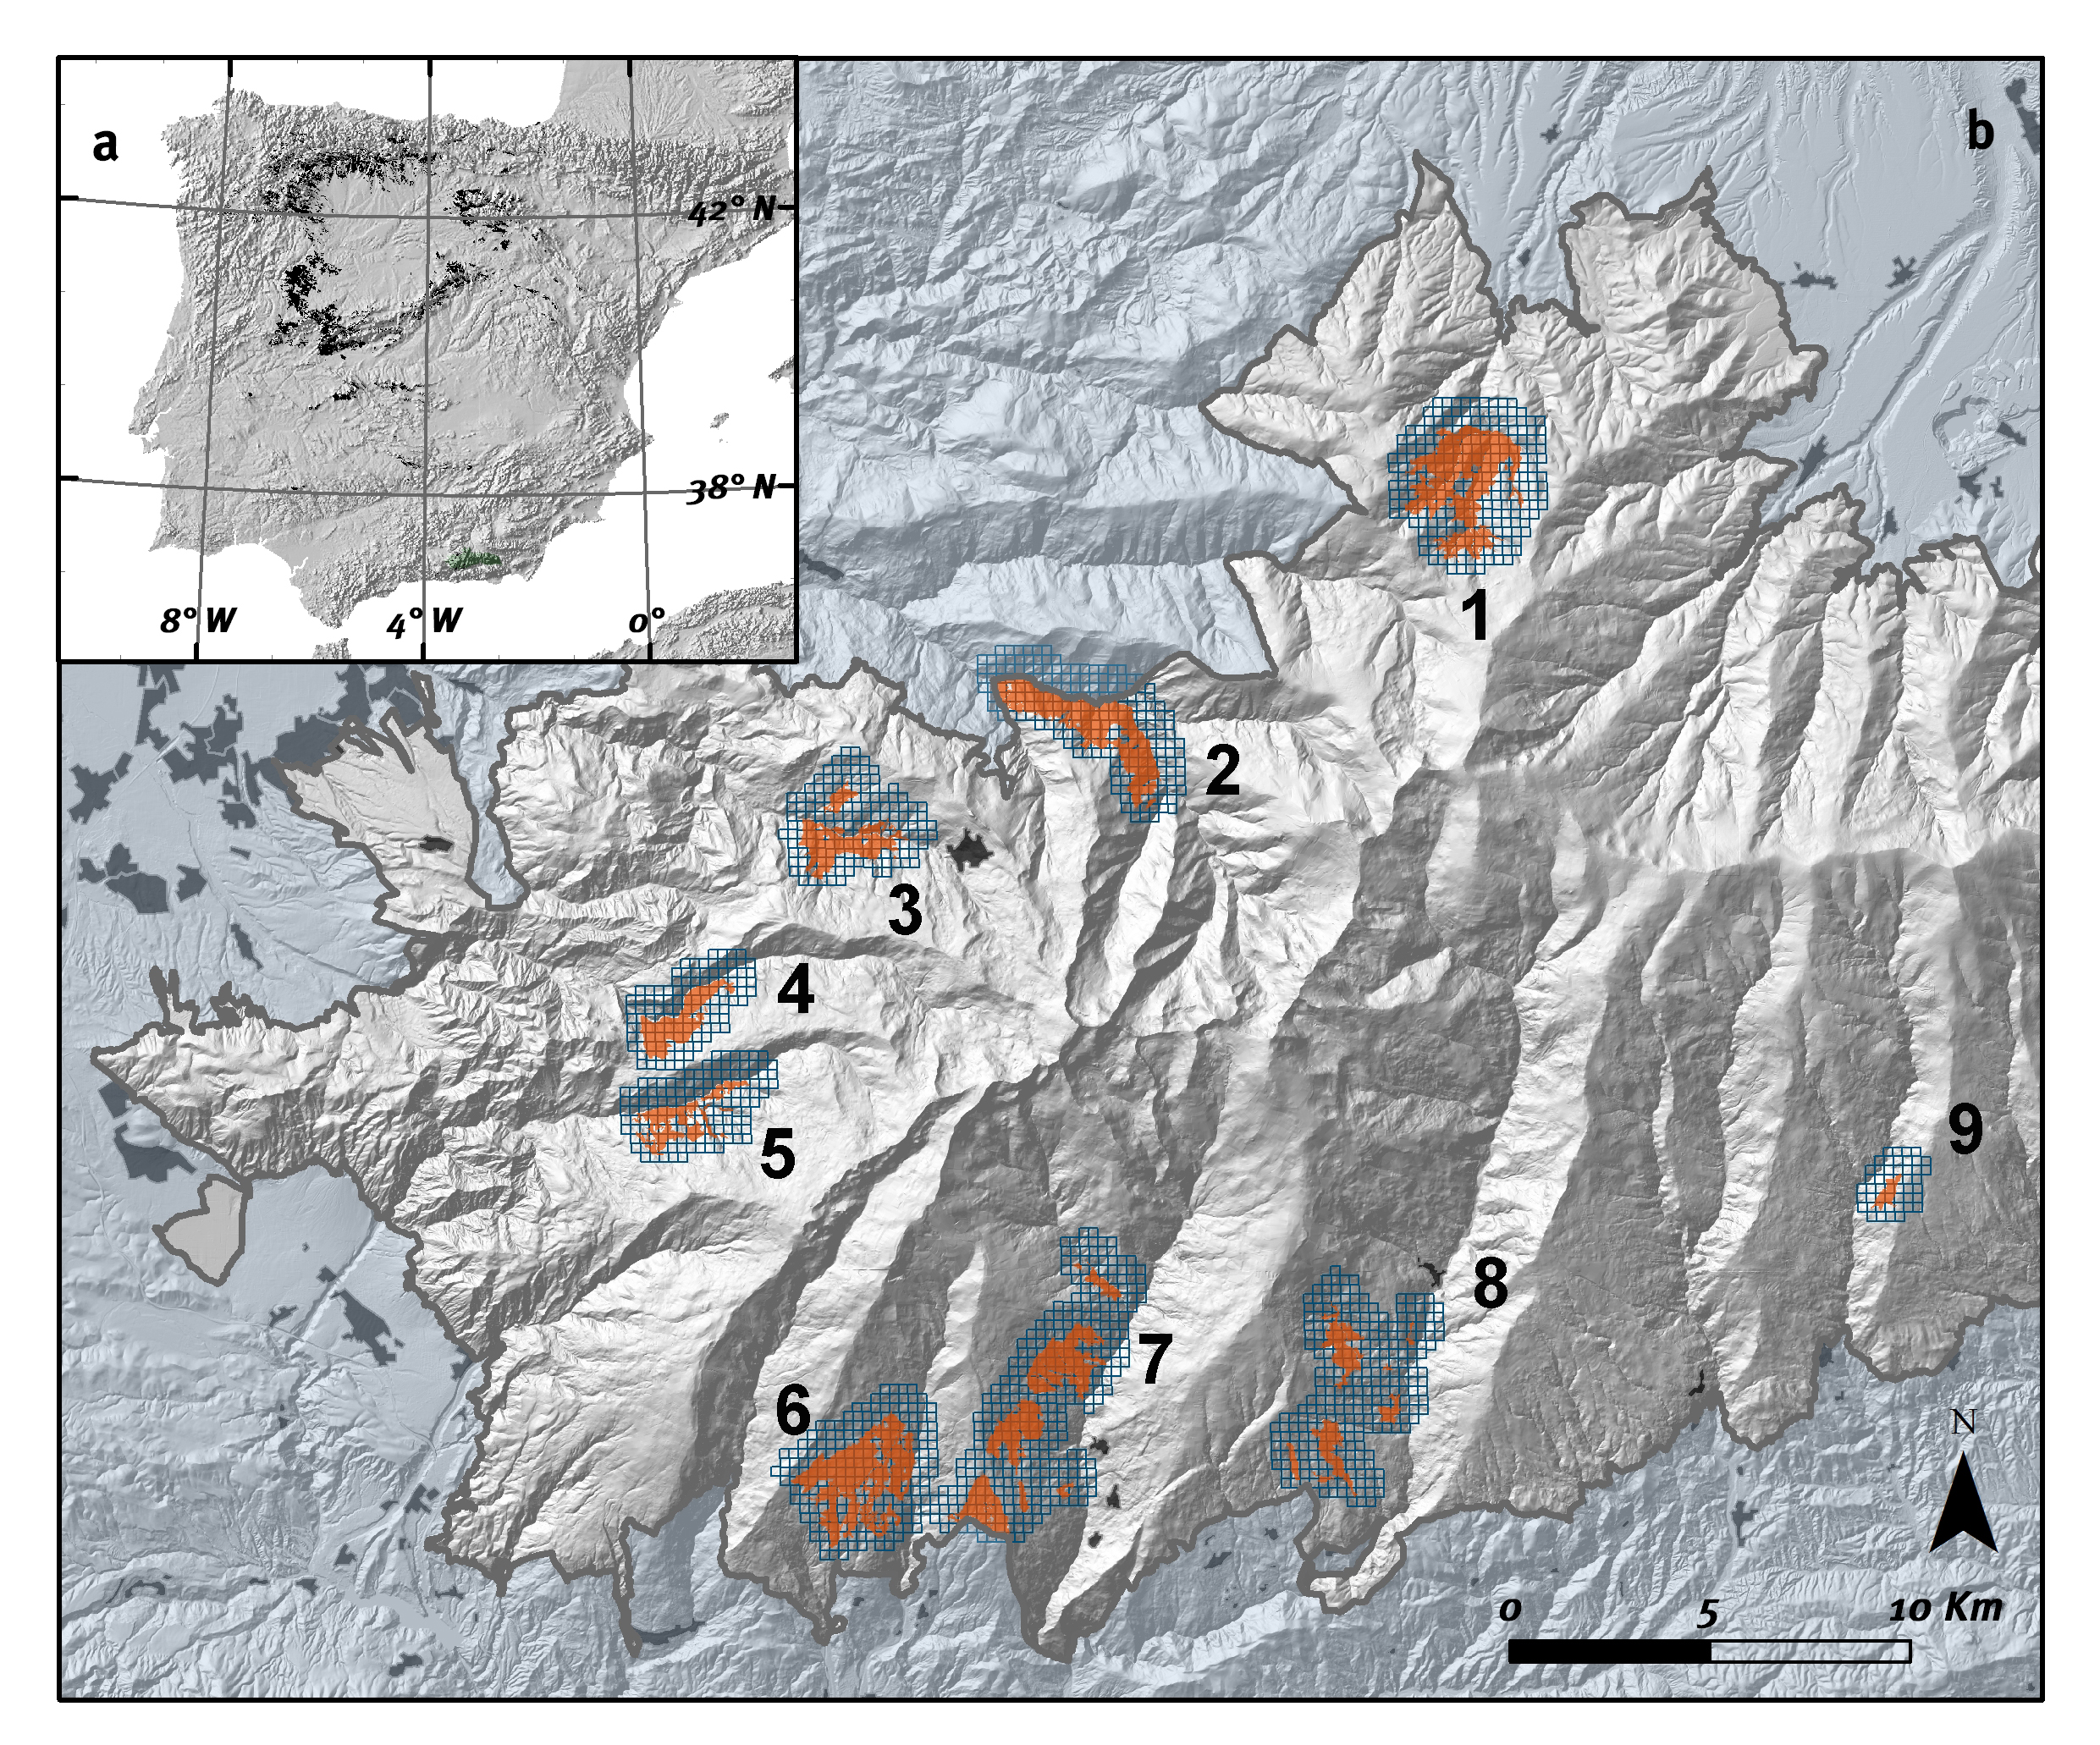
\includegraphics[width=0.7\textwidth]{img/onto/onto-location}\caption{Location of Sierra Nevada mountains. The distribution of \Qpy in the Iberian Peninsula is shown in black (\textbf{a}). The patches of \Qpy in Sierra Nevada are shown in orange (\textbf{b}). The grey line shows the boundary of the natural protected area of Sierra Nevada. The pixels used to compute the vegetation and snow indicators are included (blue grid).}\label{fig:onto:locate}
\end{figure}

\Qpy is considered as vulnerable in southern Spain \autocite{Viveroetal2000QuercusPyrenaica} and the populations inhabiting Sierra Nevada are considered relict forests \autocite{MelendoValle2000EstudioComparativo}. They have undergone intensive anthropic use in recent decades \autocite{CamachoOlmedoetal2002AltaAlpujarra}. They are also expected to suffer the impact of climate change, due to their climate requirements (wet summers): \Qpy requires between 650 and 1200 mm of annual precipitation and minimal summer precipitation between 100 and 200 mm. Thus, simulations of the climate-change effects on this habitat point to a reduction in suitable habitat for Sierra Nevada \autocite{Benito2009EcoinformaticaAplicada,Benitoetal2011SimulatingPotential}.

\subsection{Data sets and derived information}\label{sec:onto:Data}

We have selected two MODIS products: MOD13Q1 to assess the habitat functioning and MOD10A2 to study the behaviour of an abiotic factor (snow cover). MOD13Q1 provides information on vegetation index NDVI (Normalized Difference Vegetation Index). The spatial resolution of this product is 250 m and the temporal resolution is 16 days. MOD10A2 provides information about snow cover extent \autocite{Halletal2002MODISSnowcover}. It has a periodicity of 8 days and a spatial resolution of 500 m. Each MOD10A2 pixel is labelled as snow if it has had snow on one of the previous 8 days. We selected MODIS products because both their spatial resolution and temporal resolutions are appropriate for the scope of this study.
We homogenized the different spatial and temporal resolutions in these two products to produce the final data at 500 m of spatial resolution and 16 days of temporal resolution. For the spatial resolution, we intersected the two grids to assign the identifier of any MOD10A2 pixel to its overlapping one in MOD13Q1. For temporal homogenization, we aggregated the data from MOD10A2 (8 days) to gain information regarding at least MOD13Q1 scale (\emph{i.e.} more than 16 days). We used the MODIS time series from 2000 to 2012.

NDVI seasonal measurements (aggregation of NDVI values by season) are suitable tools to quantify productivity and biomass \autocite{Runningetal2004ContinuousSatelliteDerived,Turneretal2006EvaluationMODIS}, seasonality \autocite{Pineiroetal2006SeasonalVariation, PotterBrooks1998GlobalAnalysis} and other phenological measurements \autocite{Clelandetal2007ShiftingPlant}. These measurements have been used to characterize ecosystem functioning \autocite{Cabelloetal2012EcosystemFunctioning}. We have calculated indicators regarding these ecological functions using the mean NDVI profiles provided by MODIS (\figref{fig:onto:indicator}) \emph{sensu} \textcite{AlcarazSeguraetal2009BaselineCharacterization}:

\begin{itemize}
\item
  \textit{annual} and \textit{seasonal mean} (NDVI-I) which can be used to estimate fAPAR (Fraction of Absorbed Photosynthetically Active Radiation) \autocite{Sellersetal1996RevisedLand} and thus net primary production \autocite{Parueloetal1997ANPPEstimates,Sellersetal1992CanopyReflectance,Tuckeretal1985AfricanLandCover}.
\item
  \textit{annual relative range} (RREL); difference between maximum and minimum NDVI divided by annual mean. This variable provides an indicator of the seasonality of the photosynthetic activity \autocite{ParueloLauenroth1995RegionalPatterns}.
\item
  \textit{maximum} and \textit{minimum NDVI values} (MAX and MIN) and \textit{months} (MMAX and MMIN) in which they occur. They provide an additional description of phenology, indicating the intra-annual distribution of the periods with maximum and minimum photosynthetic activity \autocite{HoareFrost2004PhenologicalDescription,Lloyd1990PhenologicalClassification}.
\end{itemize}

NDSI (Normalized Difference Snow Index) is a spectral band ratio that takes advantage of the fact that snow reflectance is high in the visible wavelengths and low in the shortwave infrared region \autocite{SalomonsonAppel2006DevelopmentAqua}. This index has proven to be a robust indicator of snow cover using MODIS images\autocite{Rittgeretal2013AssessmentMethods}. We have calculated several indicators from MOD10A2 images \autocite{WangXie2009NewMethods} (\figref{fig:onto:indicator}):

\begin{itemize}
\item
  \textit{snow-cover duration} (SCD): is defined as the number of days covered by snow per hydrological year (describe a time period of 12 months for which precipitation totals are measured).
\item
  \textit{snow-cover onset dates} (SCOD): is defined as the first date in the hydrological year that the pixel has snow. This indicator is useful to identify shifts in the starting of snow season.
\item
  \textit{snow-cover melting dates (SCMD)}: is the last date in the hydrological year that the pixel has snow. This indicator provides useful information about the melting process.
\item
  \textit{snow-cover melting cycles (SCMC)}: number of melting cycles in each pixel per hydrological year.
\end{itemize}

\begin{figure}
    \centering
    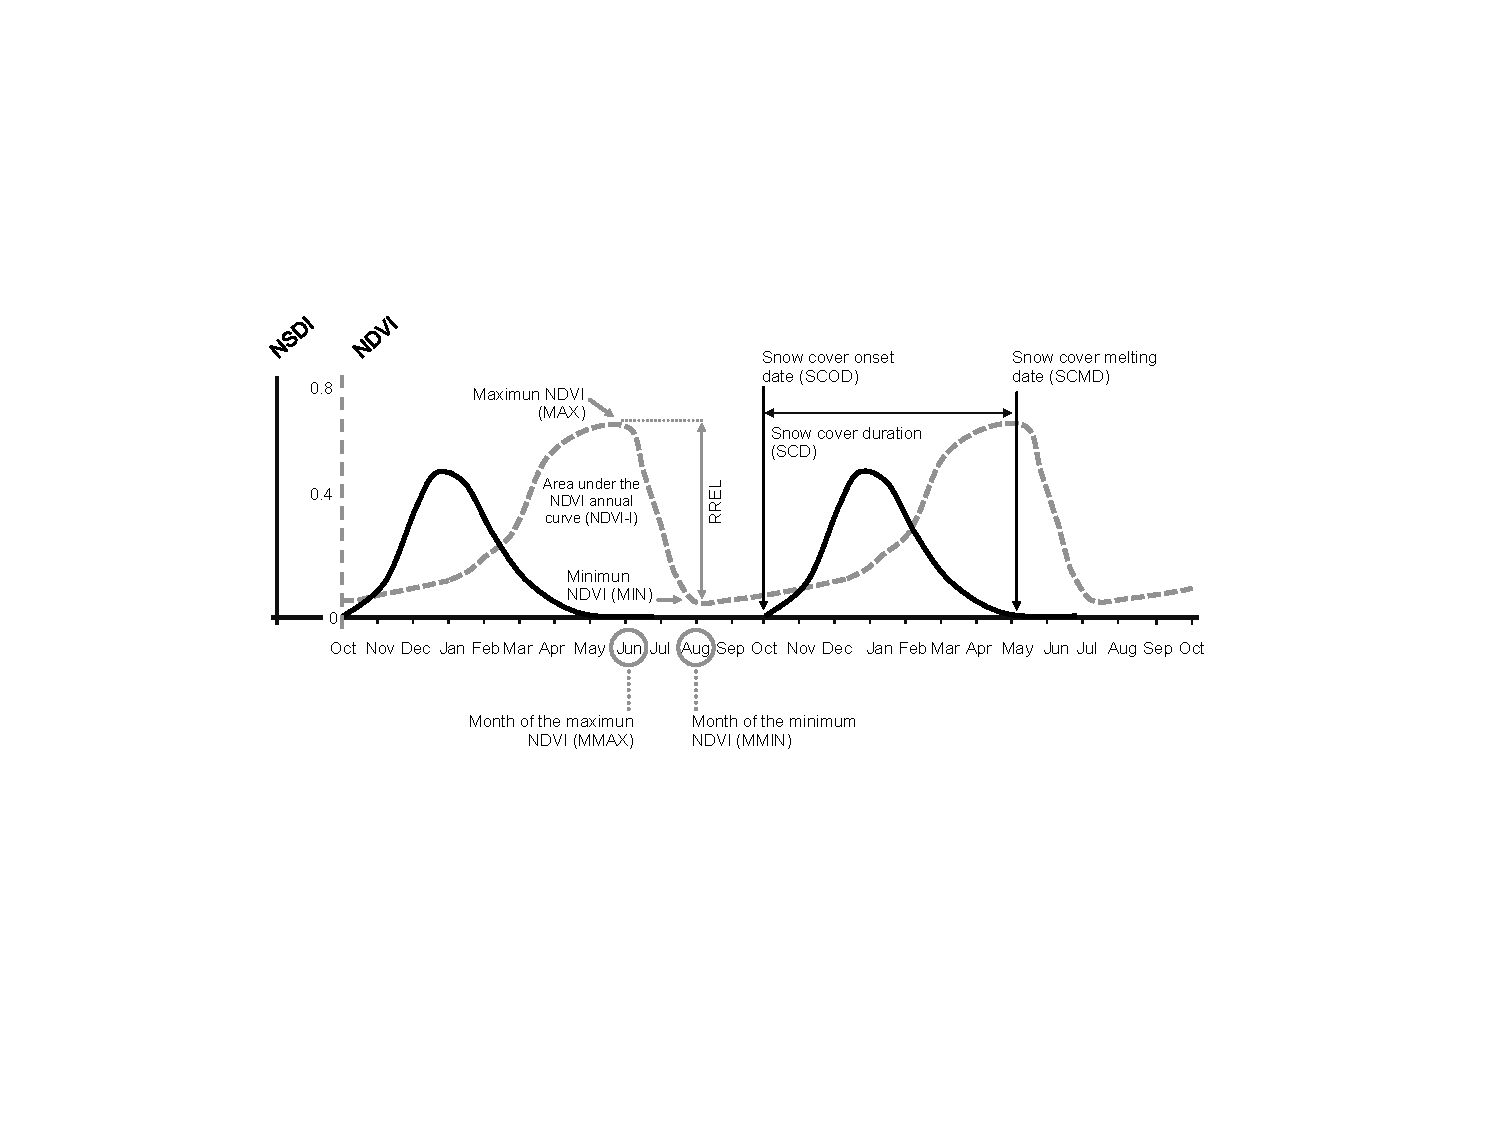
\includegraphics[width=\textwidth]{img/onto/onto-figure-indicators}\caption{Attributes derived of Normalized Difference Vegetation Index (NDVI) and snow-cover profiles. Modified from \autocite{AlcarazSeguraetal2009BaselineCharacterization,WangXie2009NewMethods}.}\label{fig:onto:indicator}
\end{figure}

\section{Knowledge retrieval: ontologies and semantic processing}\label{sec:onto:Semantic}

Savia was designed taking into account a client-server architecture (\figref{fig:onto:architecture}). The system contains different modules that extract relevant knowledge from the raw data. These modules act in a user-transparent way and are detailed in the following subsections, highlighting image processing, the development of the ontology, how instances are generated, and the final query system.

\begin{figure}
    \centering
    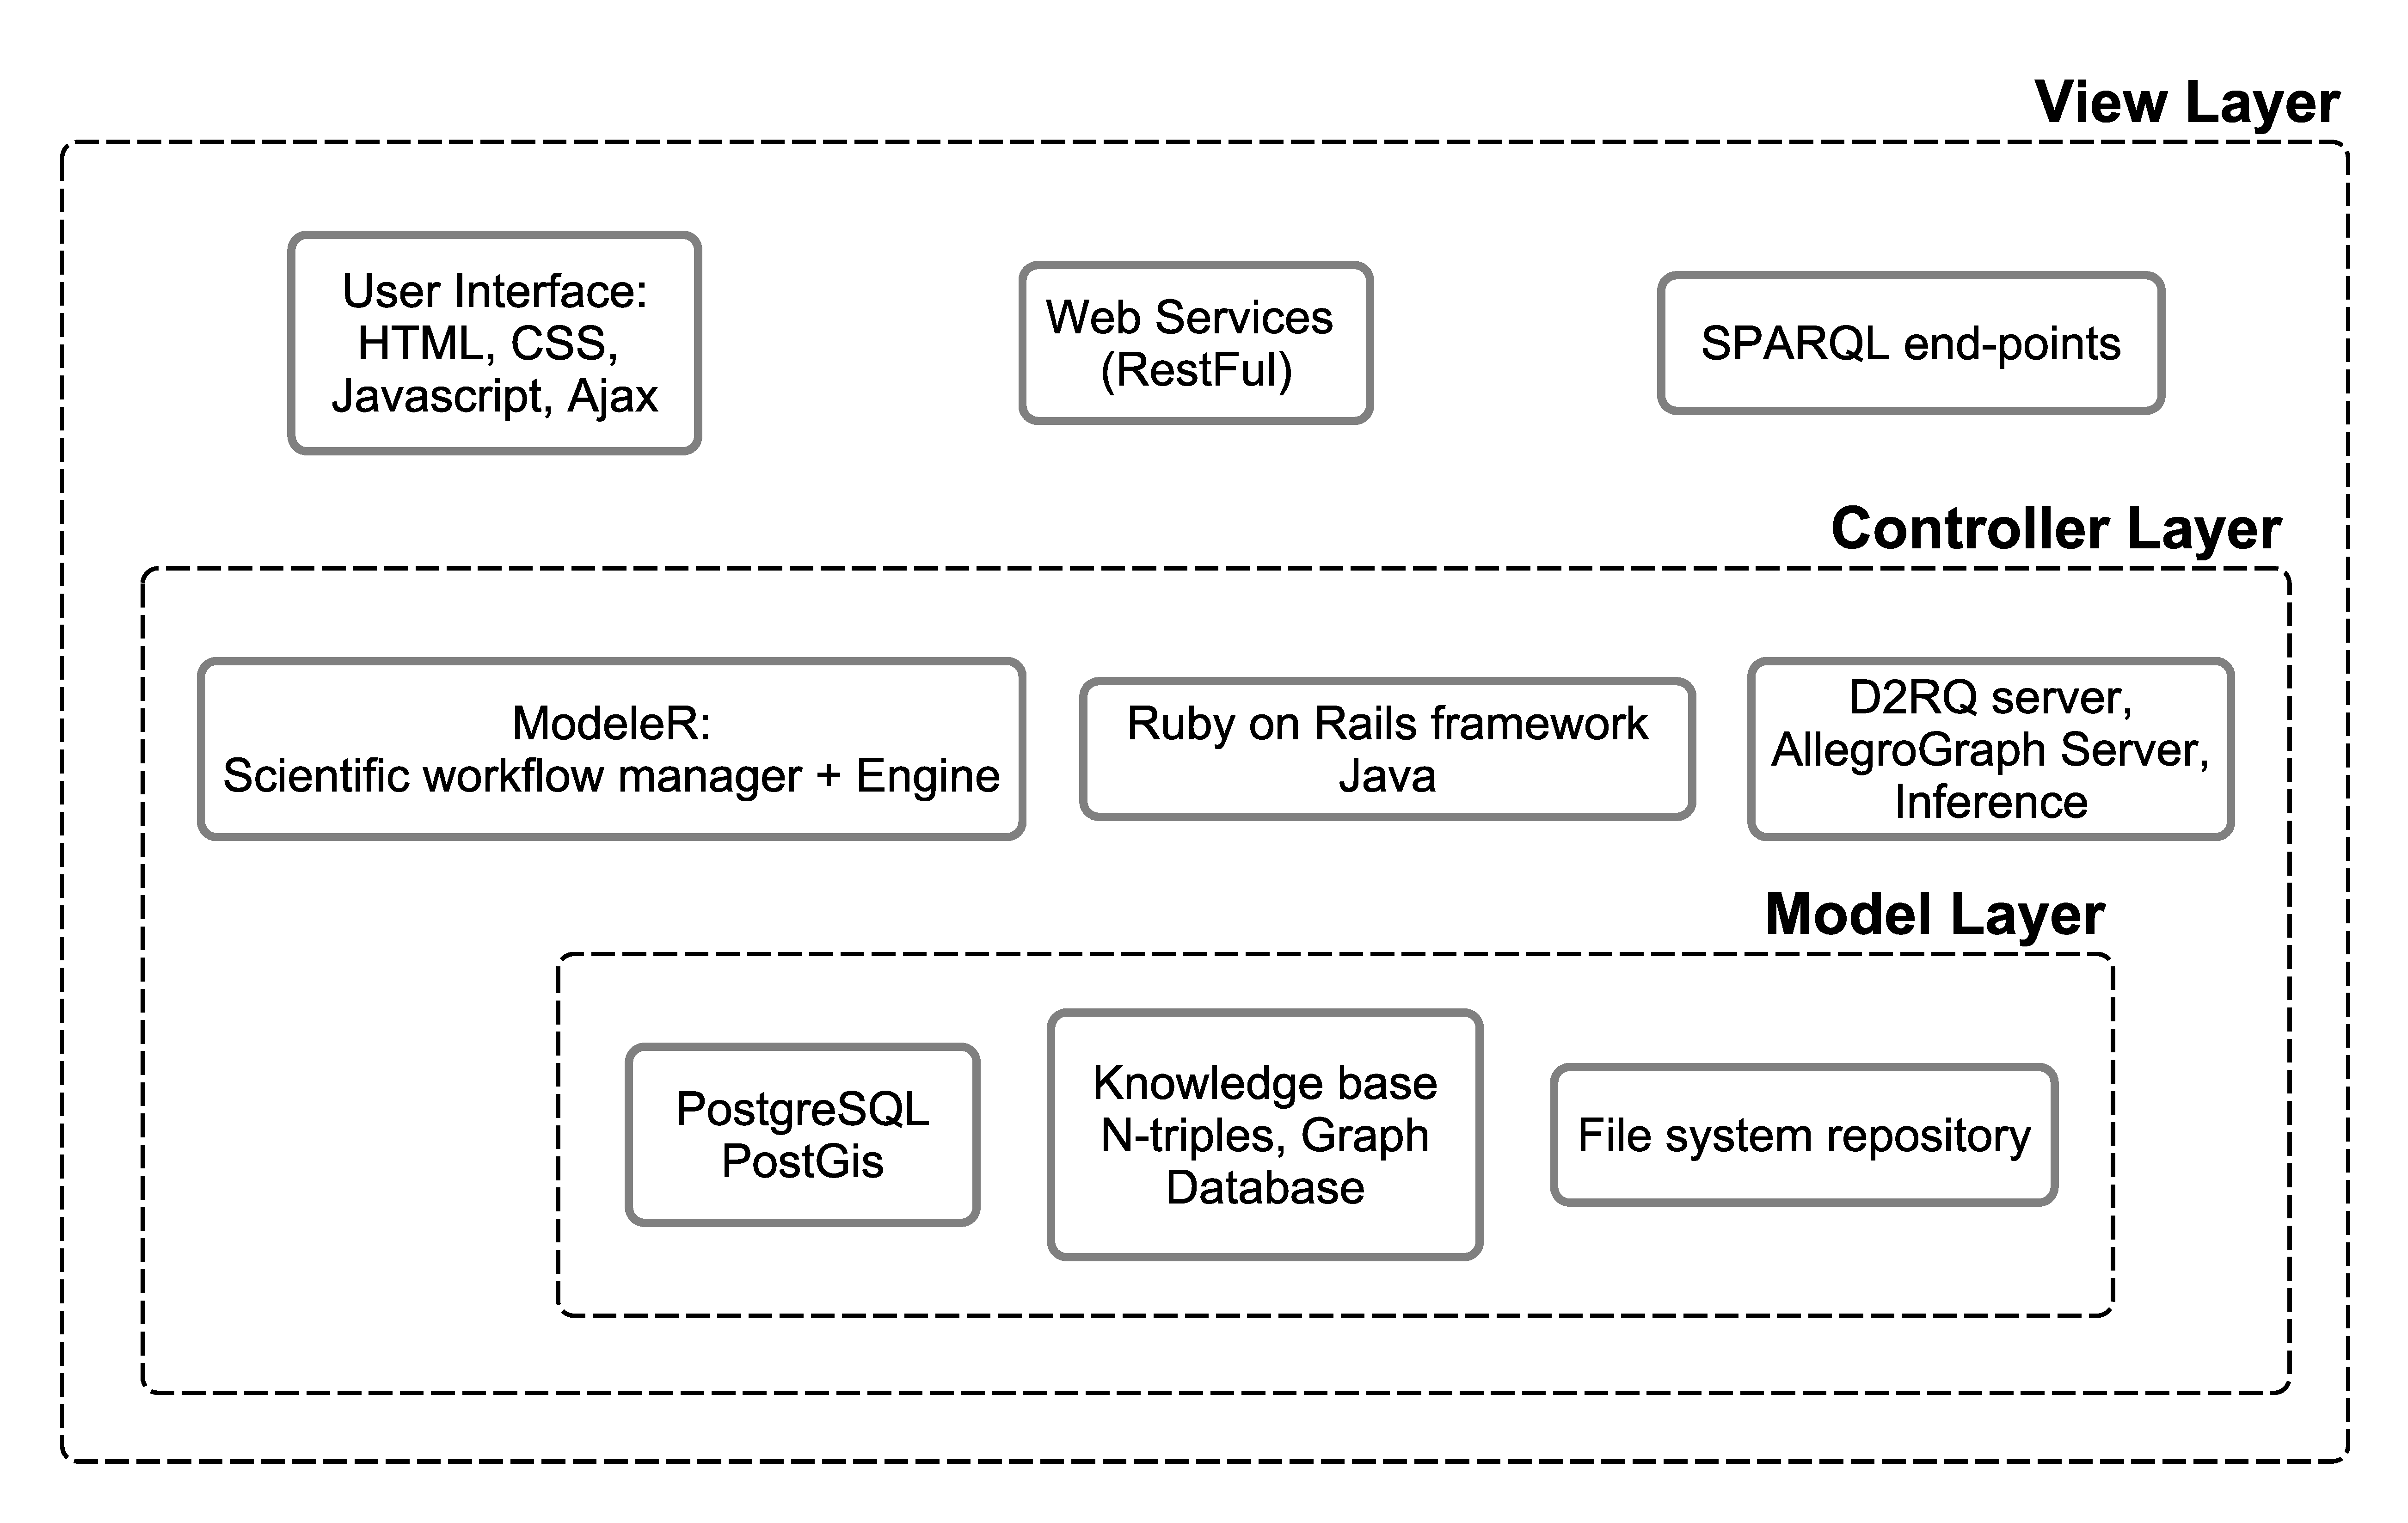
\includegraphics[width=\textwidth]{img/onto/onto-architecture}\caption{System architecture.}\label{fig:onto:architecture}
\end{figure}

subsection{Embedding MODIS images in a database and calculating thematic indicators}\label{sec:onto:Embedding}

HDF (Hierarchical Data Format) files are downloaded from NASA servers and processed using a workflow that makes the process automatic and reproducible. This workflow is stored and documented in a model repository called ModeleR \autocite{Bonetetal2014DocumentingStoring,PerezPerezetal2012ModeleREnviromental}. The workflow extracts information contained in any HDF files and stored it in a relational database (see structure in \figref{fig:onto:database}). NDVI and NDSI values are stored in a table that is linked to a vector layer containing the centroids of MODIS pixels. These raw data are used to aggregate and calculate the different indicators in Savia. The results are integrated again into the relational database, that is part of the Sierra Nevada LTER site information system \autocite{BonetGarciaetal2011SierraNevada}.\\
The indicators described in Section 2.2 were calculated for each pixel and temporal stage (by hydrological year, \emph{i.e.} the period between October 1st of one year and September 30th of the next; and by season) using SQL queries. The temporal trend for each pixel was calculated using the nonparametric Mann-Kendall trend test \autocite{Kendall1970RankCorrelation,Mann1945NonparametricTests}. The analyses were computed in R \autocite{base} with Kendall package \autocite{McLeod2011KendallKendall}. We set 0.05 the alpha level for the test, and slopes with p-values \textgreater{} 0.05 were considered significant.

\begin{sidewaysfigure}
\centering
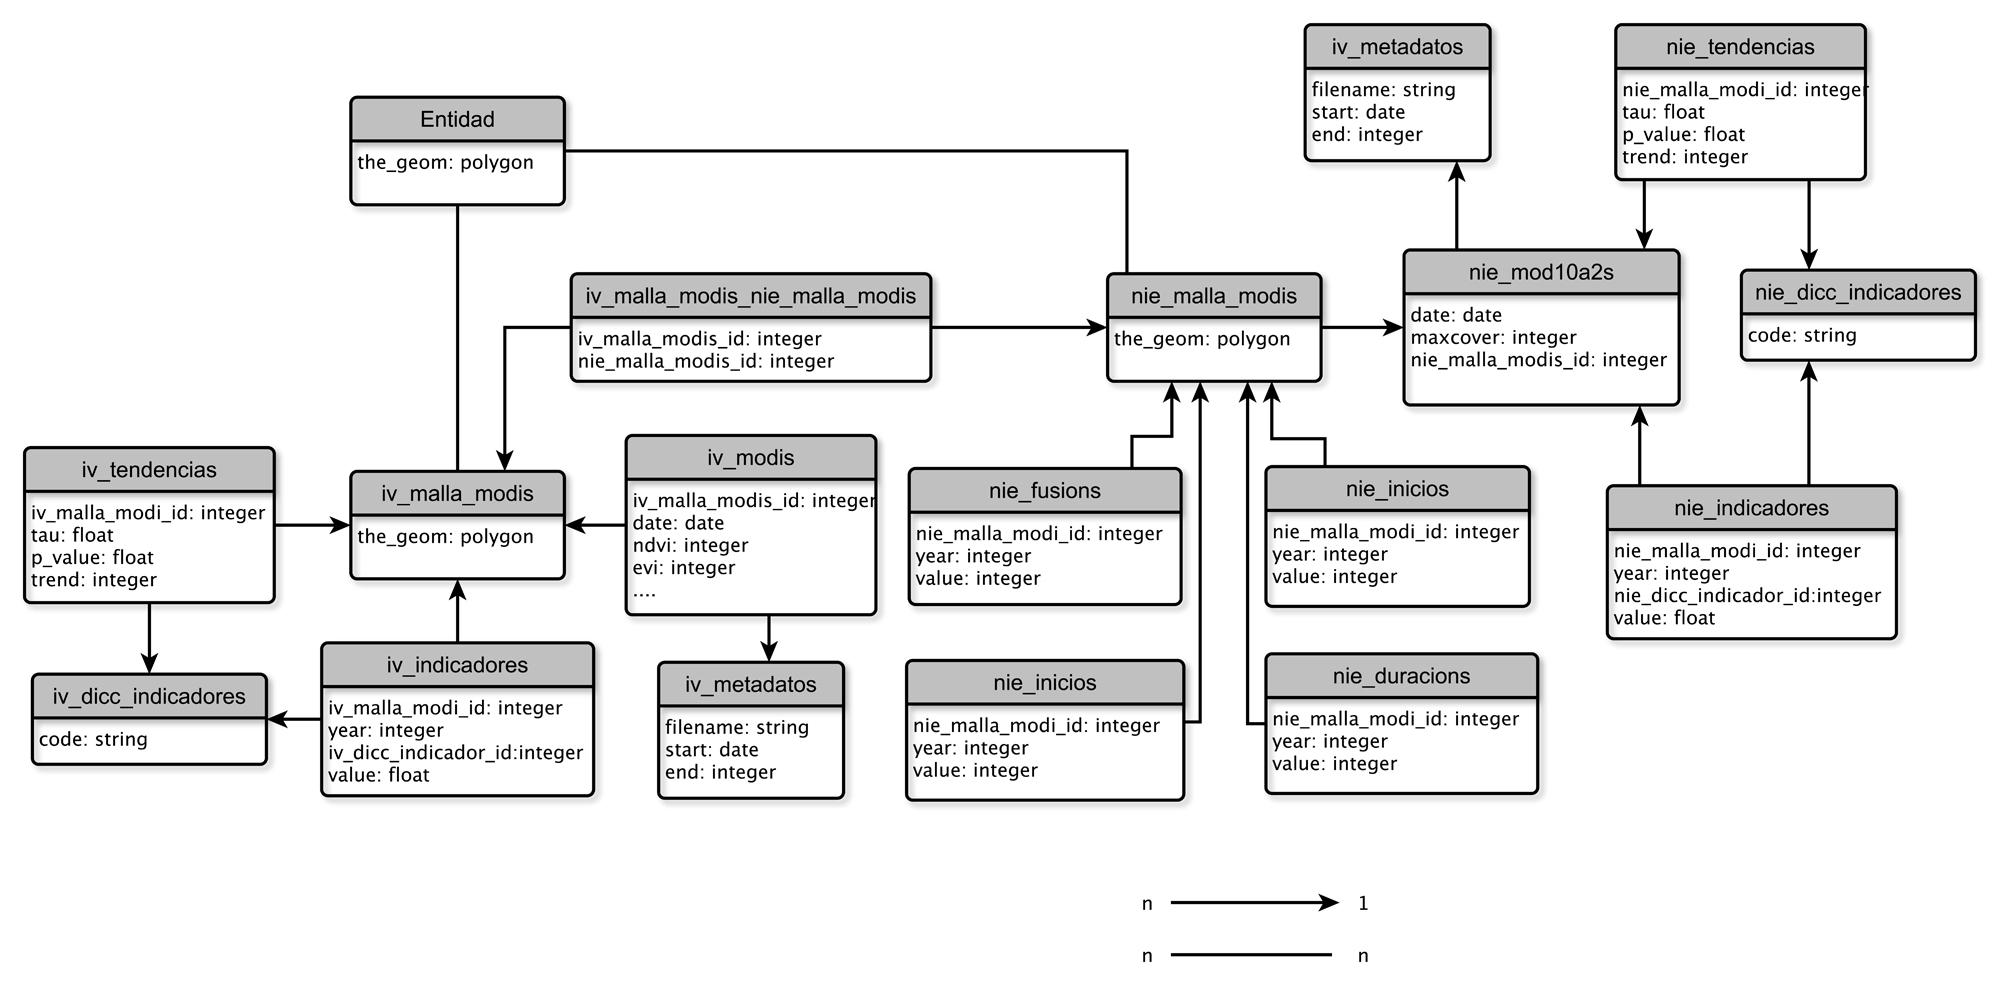
\includegraphics[]{img/onto/onto-database}\caption{Database schema. For each MODIS product the relational model stores three types of information: (i) spatial distribution of the pixels (\emph{nie\_malla\_modis} and \emph{iv\_malla\_modis} tables); (ii) values of NDVI and NDSI from original HDF files (\emph{nie\_mod10a2s} and \emph{iv\_modis} tables); and (iii) the metadata associated with each original image (\emph{nie\_metadatos\_modis} and \emph{iv\_metadatos} tables). The database also contains an auxiliary table to manage spatial entities (\emph{i.e.} \Qpy patches). Finally, there was a set of tables containing the aggregated information and indicators obtained after processing the raw data (see Section 2.2) (tables \emph{iv\_tendencias}, \emph{iv\_indices}, \emph{nie\_inicios}, \emph{nie\_fusions}, \emph{nie\_tendencias})}\label{fig:onto:database}
\end{sidewaysfigure}

\subsection{Creating the ontology}\label{sec:onto:Creating}

The ontology must represent both the information (MODIS products, indicators, and temporal trends) and the concepts used to add ecological meaning to the data (\figref{fig:onto:ontology}). To build the ontology, we used Time Ontology in OWL (Web Ontology Language) \autocite{HobbsPan2004OntologyTime} and Basic Geo (WGS84 lat/long) Vocabulary \autocite{Brickley2003BasicGeo} external ontologies. The OWL-Time ontology promoted by W3C (World Wide Web Consortium) \autocite{W3C2013LargeTriple}, provides a vocabulary for expressing instants and intervals, together with information concerning durations and date/time information \autocite{HobbsPan2004OntologyTime}. The Basic Geo is an RDF (Resource Description Framework) vocabulary for representing latitude, longitude, altitude information as well as other information related to spatial-located items.

Thus, the ontology takes into account three different parts (\figref{fig:onto:ontology}):

\begin{enumerate}
    \item Representing spatial information. The main concept is the Pixel, which represents a pixel from a MODIS image. Some pixels that share similar functions (\emph{i.e.} be covered by the same habitat) may belong to a Patch. Finally, some patches sharing the same dynamics may belong to a Group. The properties called \emph{PixelBelongsToPatch} and \emph{PatchBelongsToGroup} help to define the relationships between the previously defined concepts. \emph{PixelIsNearTo} is another useful property that adds the functionality of proximity to any pixel. The distance threshold used was 500 m between pixels (500 m is the spatial resolution of MODIS snow products). This property is symmetric because when a pixel A is near B, B is also near A.
    \item Indicators. This part contains a concept (\emph{IndicatorValues}) that represents the different values that take an indicator (see Section 2.2) at a given time point (through the concept called time: Year and the property \emph{HasYear}) and in a given place (through the concept Pixel and the property \emph{IndicatorValuesLocateInPixel}). We have also included a concept to describe all the indicators (Snow-cover duration, Snow-cover onset date, NDVI\_i annual, Maximum NDVI, etc.). These concepts are grouped according to their thematic area (Snow and Vegetation). Each indicator has a property called value that is measured using a given specific unit.
    \item The temporal trends are described in a concept called \emph{IndicatorTrend}. This concept shows the temporal trend of a single point for the whole time series (it is linked to \emph{Pixel} via \emph{PixelHasIndicatorTrends}). We have also created a concept for each temporal trend calculated for the previously described indicators (Trend of Snow cover duration, Trend NDVI\_i annual, etc.). These concepts are also grouped according to their thematic area (Snow Trend, Vegetation Trend). All these concepts have the following properties:
    \begin{enumerate}
        \item \emph{value\_tau} and \emph{p\_value}: These properties contain the statistic (\emph{value\_tau}) and the significance (\emph{p\_value}) reached by the Mann-Kendall trend analysis.
        \item \emph{value\_trend}: Categorical property ranges from -1 (significant negative trend) to 1 (significant positive trend). It is calculated according to the values of \emph{value\_tau} and \emph{p\_value.}
    \end{enumerate}
\end{enumerate}

This schema was implemented using OWL DL (Description logic) that allows an enhanced expression level and does not limit the values for cardinality \autocite{Smithetal2004OWLWeb}. The structure of the ontology created can be downloaded following this link: \url{http://iecolab.es/indicators.rdf}

\begin{sidewaysfigure}
\centering
    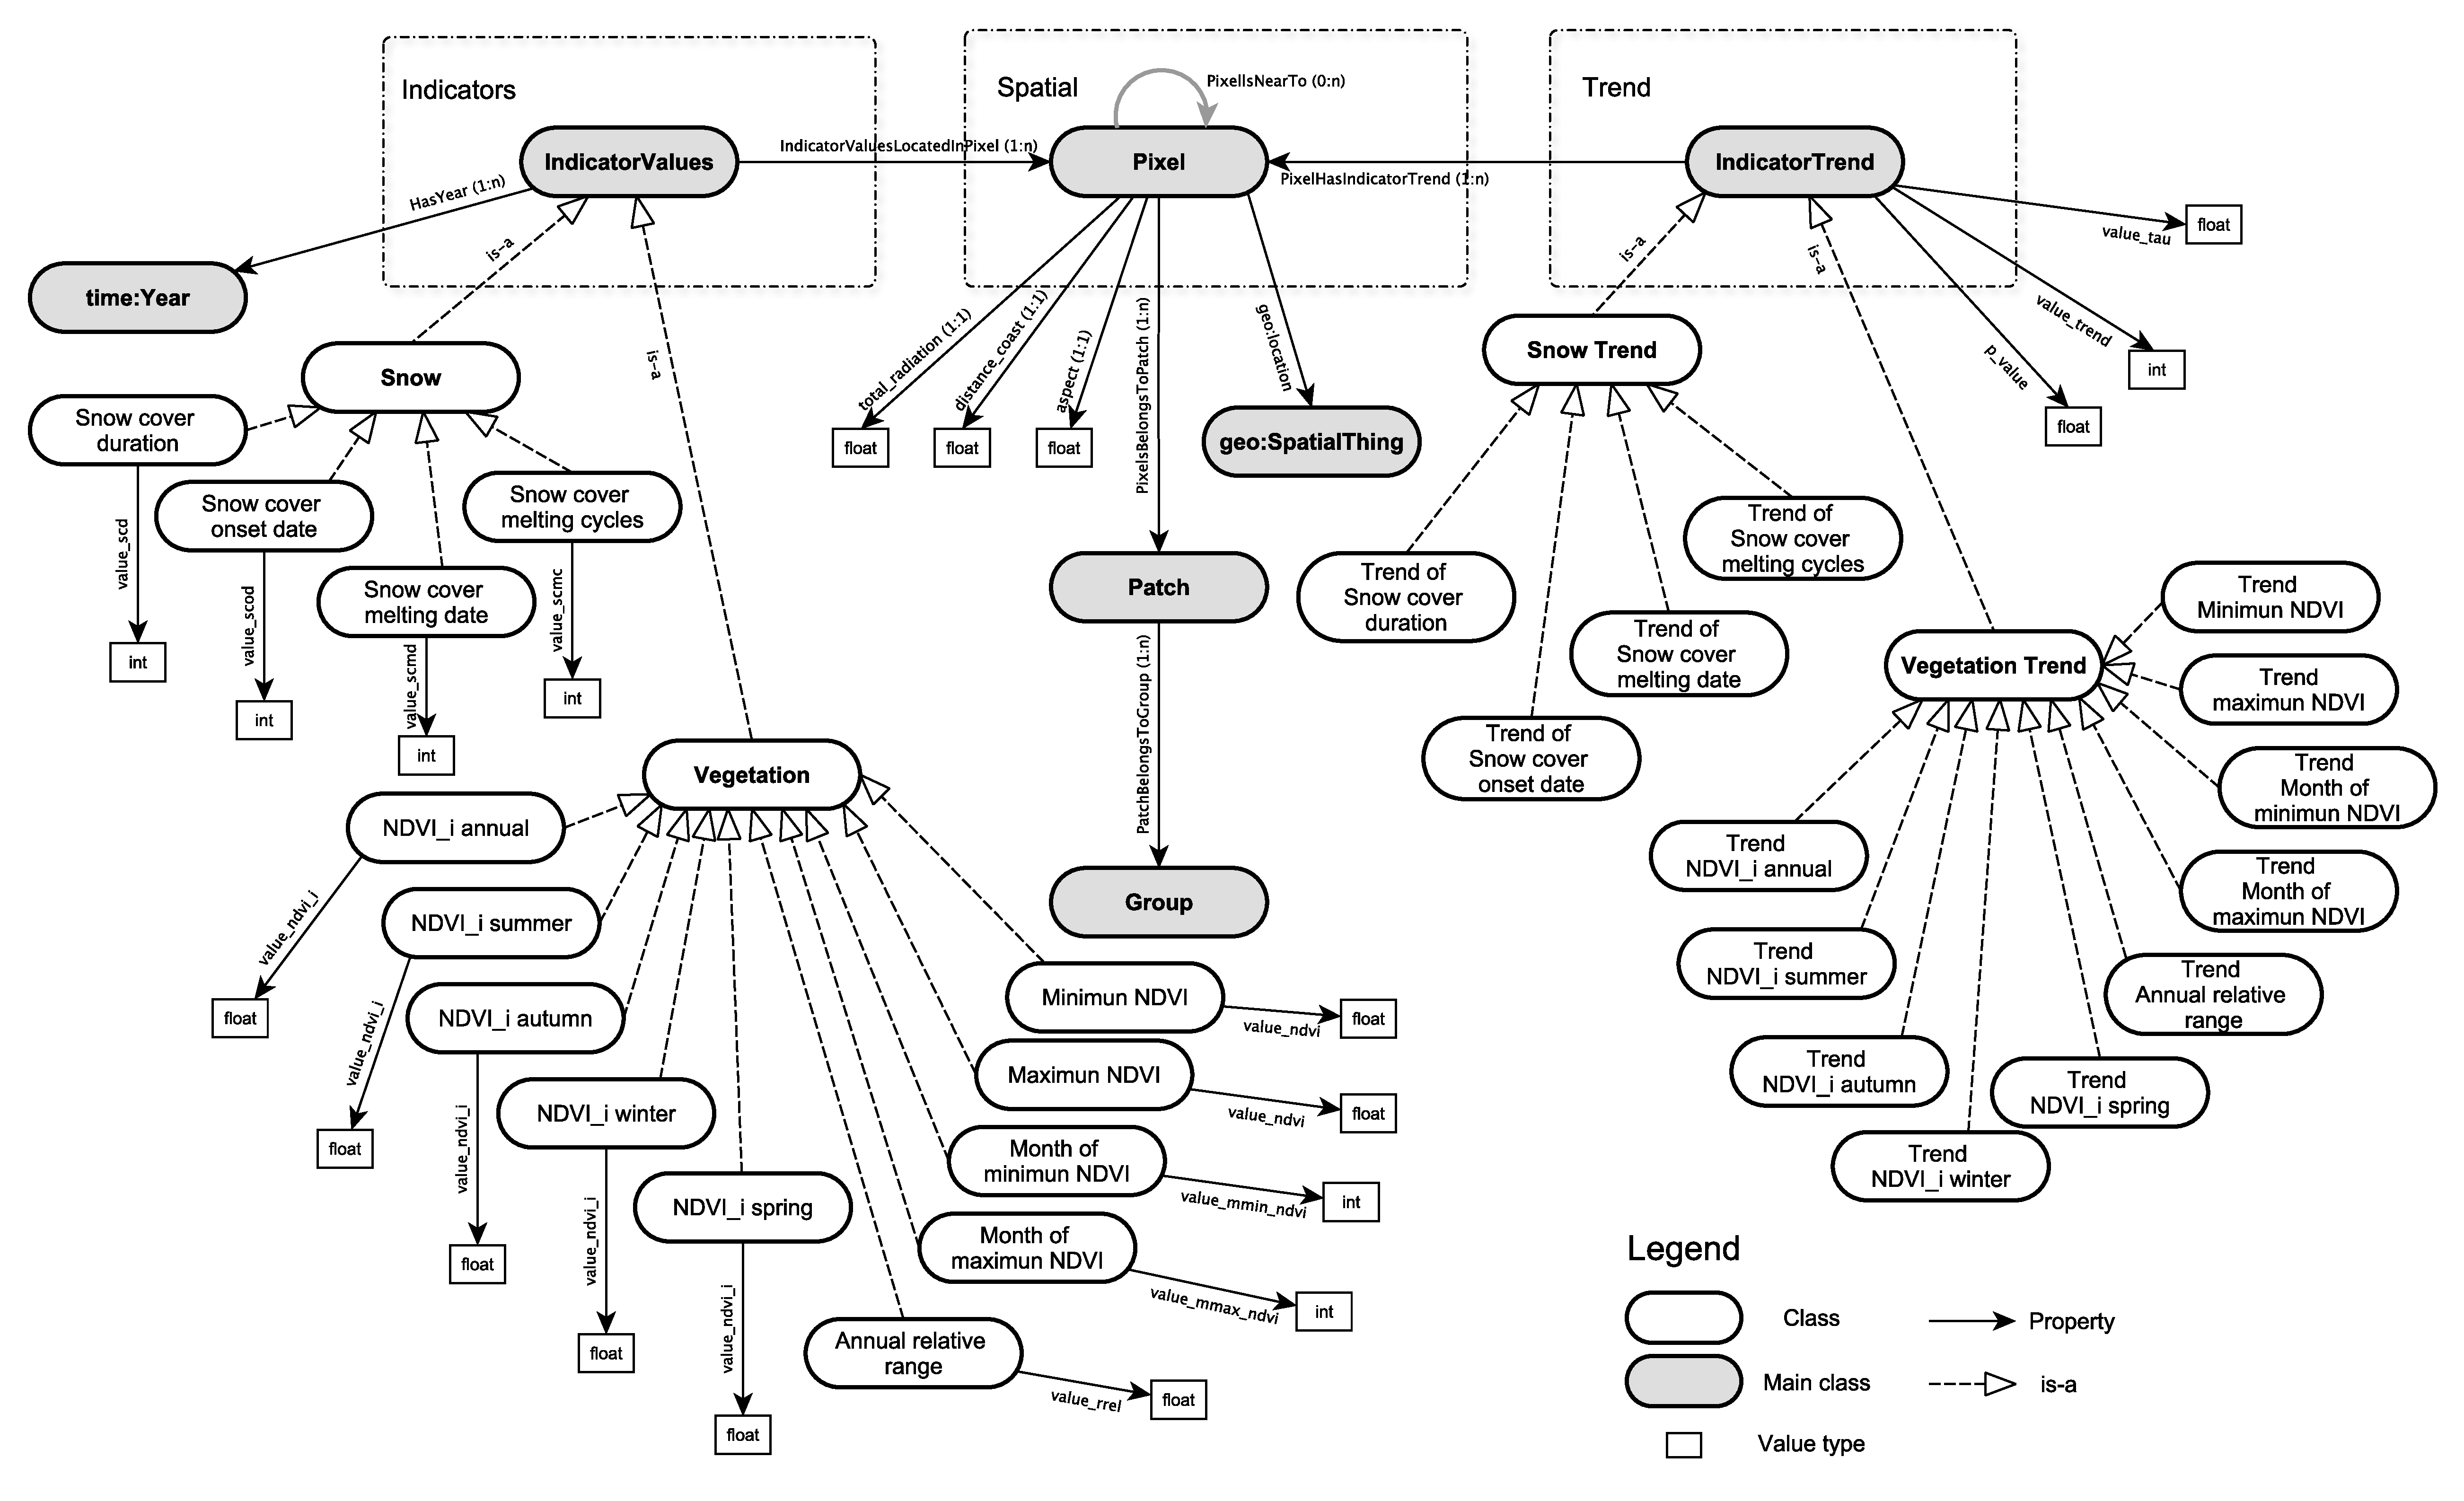
\includegraphics[width=\textwidth]{img/onto/onto-ontology}\caption{Detailed representation of the ontology created. Three main parts are considered:  spatial information, indicators, and temporal trends of the indicators}\label{fig:onto:ontology}
\end{sidewaysfigure}

\subsection{Knowledge base, SPARQL endpoint and inference}\label{sec:onto:SPARQL}

The next step after creating the ontology is to map the records in the database that contain the data to the ontology. Firstly, we used D2RQ \autocite{Bizeretal2004D2RQTreating} to map the relational database to OWL ontology. This software allows instance data to be retrieved from relational databases on-the-fly during the execution of SPARQL queries. Nevertheless, this procedure is time consuming and demands powerful computational capabilities. Thus, we dumped the mapping created with D2RQ into an intermediate N-triples file to avoid this drawback \autocite{Sarkaretal2011LinkedData}. This file was created with the data existing in the database and has all the triplets contained in the knowledge base.

To store the knowledge base, our tests with the open-source Apache Fuseki and Jena (\url{http://jena.apache.org/}) frameworks yielded unsuccessful results as soon as the data volume started to grow. Because we need an efficient implementation that can be scaled to large, enterprise-class data \autocite{Wilkinsonetal2004EfficientRDF}, we also conducted some tests with AllegroGraph (\url{http://www.franz.com/agraph/allegrograph/}) and Virtuoso (\url{http://virtuoso.openlinksw.com/}), choosing the former option because of its capabilities and user-friendly management environment. This software is a triplestore that uses a graph database and it has the ability to encode values directly into its triples.
To enhance the results of the queries, a reasoning task can be also triggered within the generation of the system output process. AllegroGraph provides a built-in inference engine that derives implicit information from the knowledge base. Thus, users can easily turn it on by toggling that option in the query builder interface to enrich their queries. The inference engine is useful to find relations on different types of indicators and other implicit properties such as \emph{PixelIsNearTo}. For example, Savia can answer questions concerning implicit knowledge of pixels with a positive trend on seasonal mean of NDVI near others with a negative trend in snow-cover melting dates.

\section{Study Case}\label{sec:onto:CaseStudy}

For the improvement of the conservation status of habitats, it is necessary to implement management plans according to the Annex 6 of the Habitats Directive. Our system provides knowledge useful to design those management plans. We have used \Qp forests in Sierra Nevada (Spain) to explore the importance of snow duration in the functioning of \Qp forests. We have chosen this habitat as a case study for two reasons: \emph{a)} its interesting ecological dynamics (deciduous forest in a Mediterranean mountain), and \emph{b)} the need to manage these forests in a global-change context.

We have structured the case study according to three questions that will provide two types of results. Some of them will help in the understanding of the ecological functioning of the target habitat. And others will demonstrate how ontologies are useful tools to make remote sensing information more accessible for non-expert users.

\subsection{Which pixels show a trend towards higher productivity in summer?}\label{sec:onto:Trends}

\Qp forests show a well-defined growth season centred in summer \autocite{Alcarazetal2006IdentificationCurrent,Dionisioetal2012SatelliteBasedMonitoring}. Some works have pointed out changes in habitat functioning: increase in annual vegetation greenness in Sierra Nevada \autocite{AlcarazSeguraetal2008TrendsSurface,AlcarazSeguraetal2010EvaluatingConsistency} and seasonal functional changes in \Qp woodlands \autocite{Marty2008RegimeShift}, during the last decade.

This question aims to explore whether our target habitat is undergoing changes in summer productivity, specifically which \Qp forests of Sierra Nevada have shown a positive trend of the value of summer productivity (summer NDVI).

\begin{sidewaysfigure}
\centering
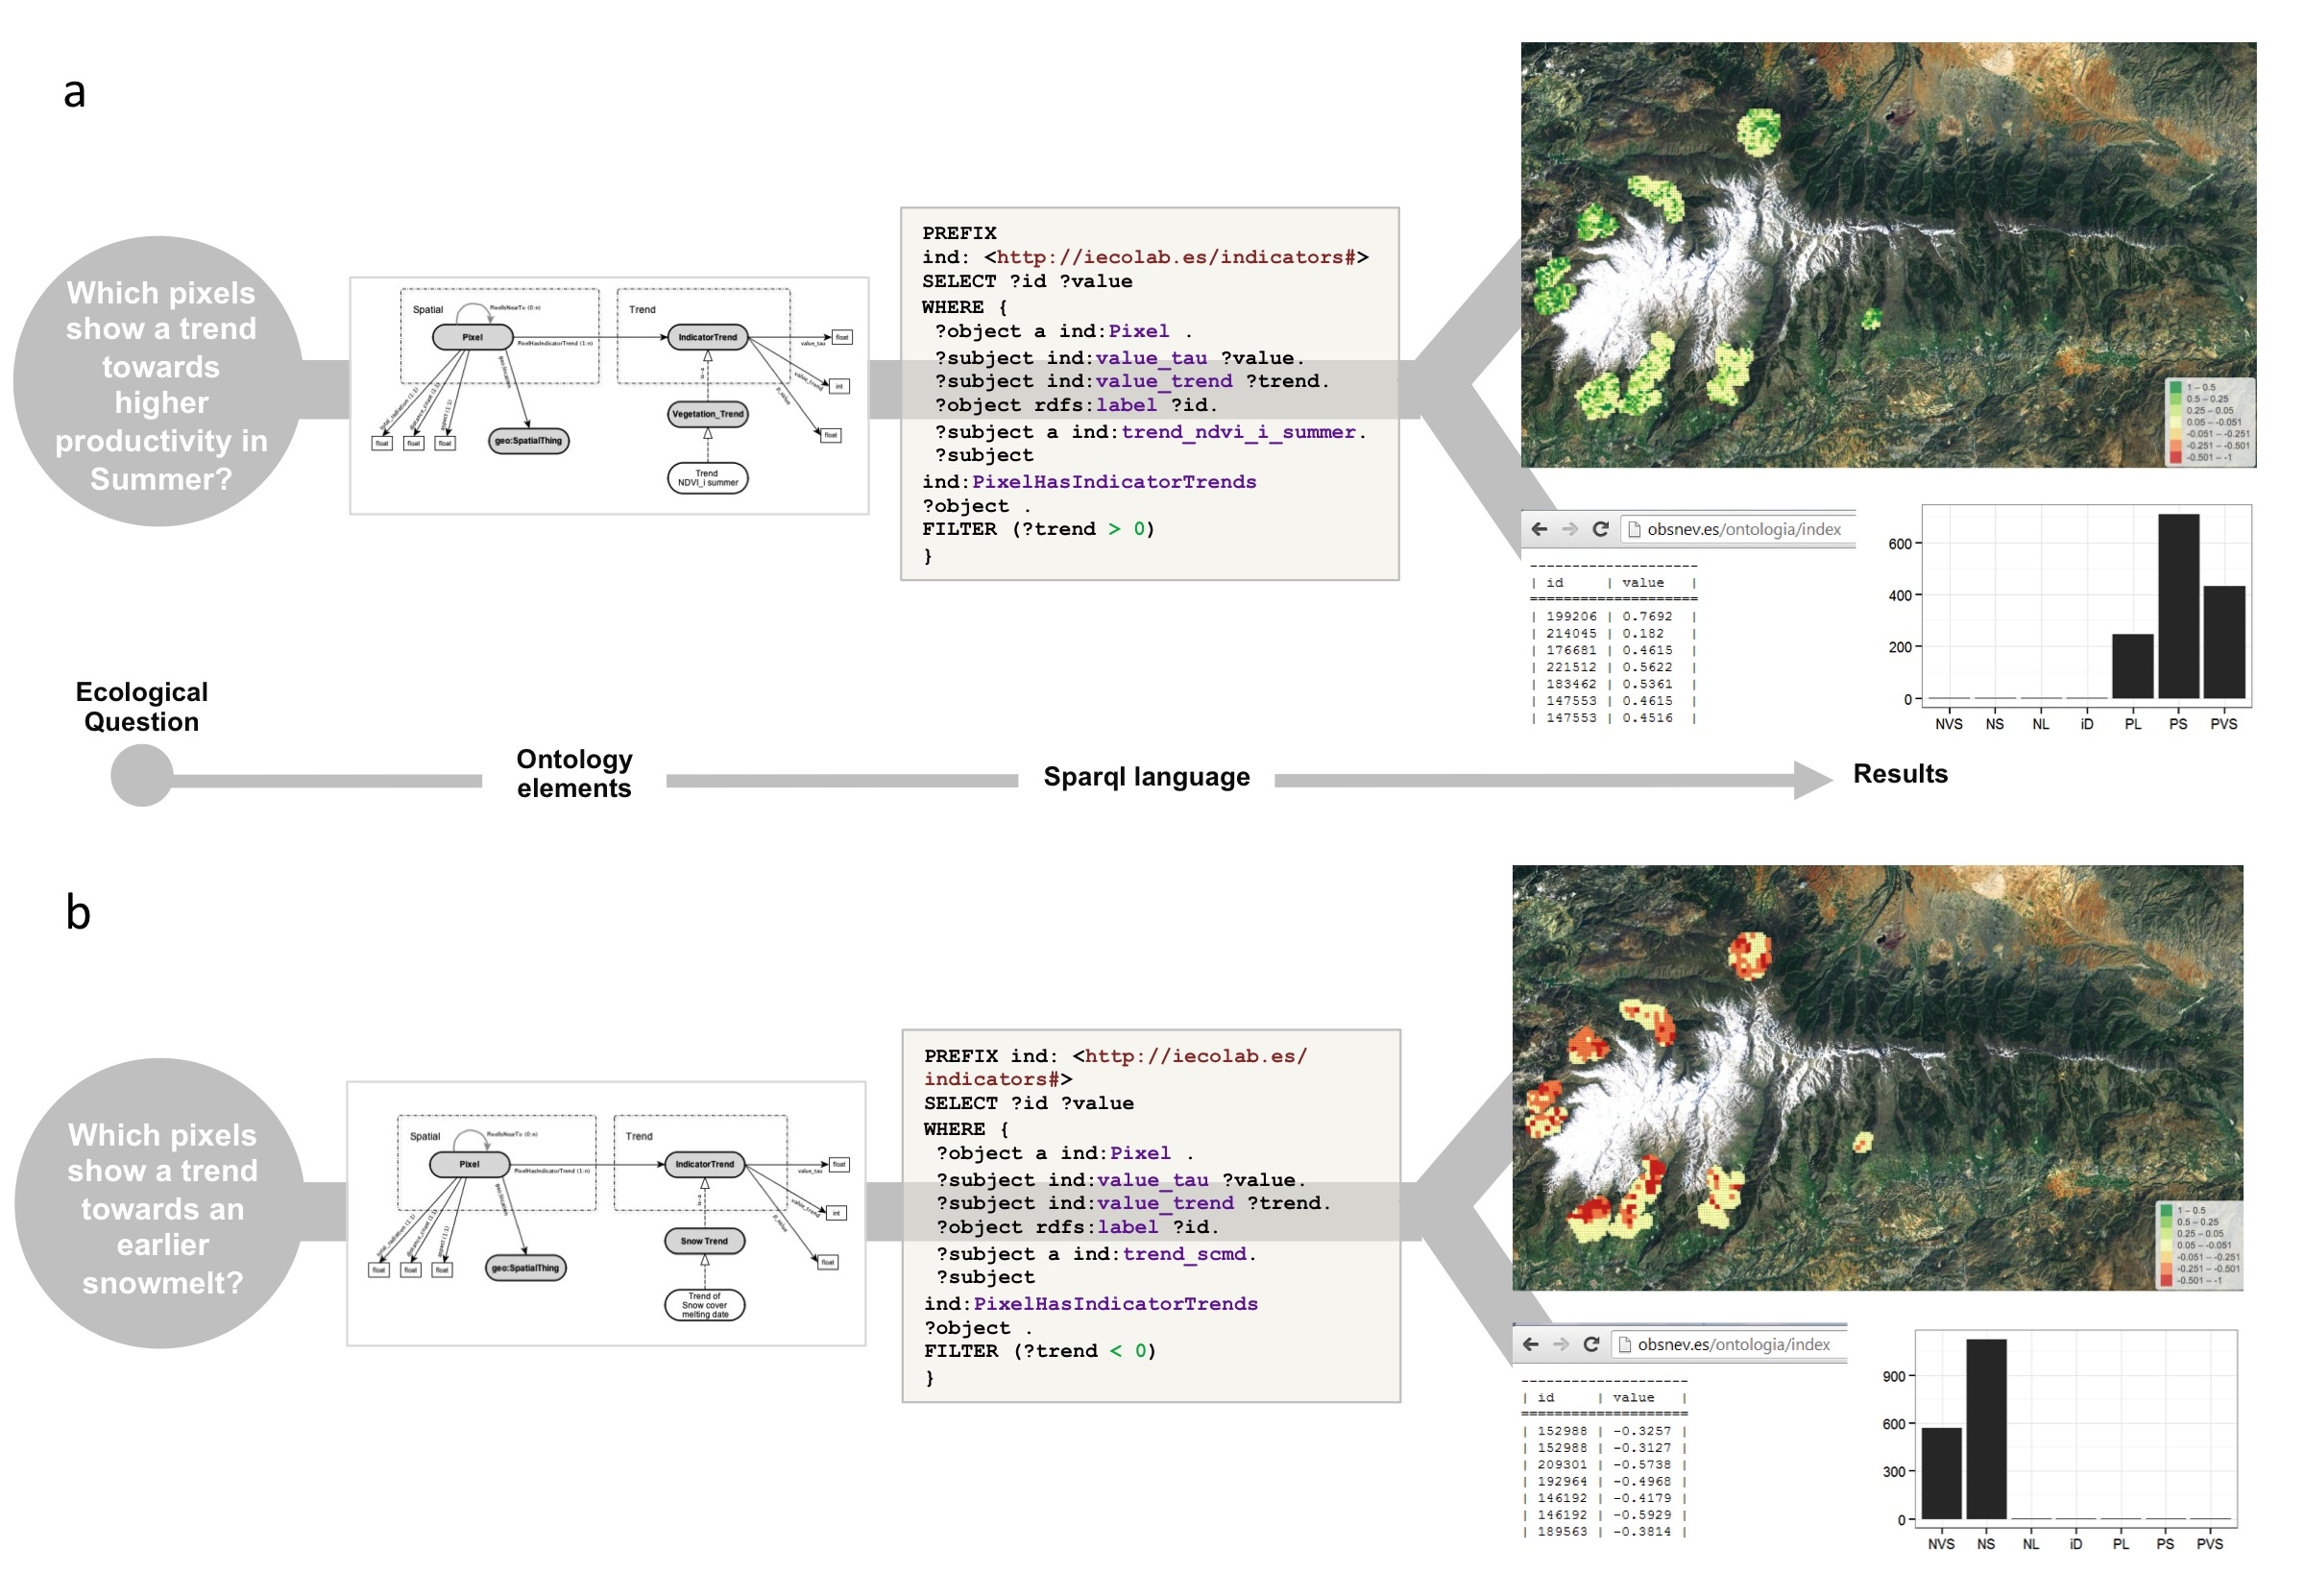
\includegraphics[width=.8\textwidth]{img/onto/onto-case-study}\caption{Scheme showing how the ontology solves questions regarding habitat functioning (a) and the behaviour of an abiotic factor (b). For each ecological question, different ontology elements are used to answer it. Then SPARQL language is used to query the knowledge base. Finally, results can be shown in different formats: map, csv or histogram. See first and second question of the study case. All pixels are displayed on the resulting map, but for those that have a significant positive trend the tau value is retrieved. In the map, we show seven different colours corresponding to this classification of tau values: [1, 0.5], [0.5, 0.25], [0.25, 0.05], [0.05, -0.051], [-0.051, -0.251], [-0.251, -0.501], [-0.501, -1].}\label{fig:onto:casestudy}
\end{sidewaysfigure}

\subsection{Which pixels show a trend towards an earlier snowmelt?}\label{sec:onto:Snowmelt}

Several studies have pointed out a trend towards higher temperatures and lower precipitation for the Mediterranean area \autocite{GarciaRuizetal2011MediterraneanWater,GiorgiLionello2008ClimateChange}. Significant declines in snow-cover extent and duration has been reported in some European mountains \autocite{Marty2008RegimeShift,MorenoRodriguezetal2005EvaluacionPreliminar,Nikolovaetal2013ChangesSnowfall,Scherreretal2004TrendsSwiss}. Climate projections forecast an increase of +4.8ºC at the end of the 21st century \autocite{Benitoetal2011SimulatingPotential} for Sierra Nevada and it expected that snowmelt will occur earlier in the year and will be more rapid \autocite{GarciaRuizetal2011MediterraneanWater}.

The second question that we raised it concerns the observed changes in snowpack in Sierra Nevada. We are interested specifically in which pixels show a trend towards earlier snowmelt during spring-summer. This question is crucial, given that \Qp forests need water in summer for growth.

\subsection{Which \Qp patches show a trend towards a more productive summer and earlier snowmelt?}\label{sec:ontoProductive}

This question explores the relationships and co-occurrence between biological production and snow-cover features.

Snow-related variables can explain the distribution of plant communities in the landscape \autocite{Jonesetal2001SnowEcology}. This causal relationship is more important at high elevation \autocite{BonetGarciaCayuela2009SeguimientoCubierta} in Sierra Nevada. But snow cover also explains part of the ecosystem functioning. \textcite{Trujilloetal2012ElevationdependentInfluence} that vegetation greenness increases with snow accumulation. This relationship varies with elevation, reaching a maximum between 2000-2600 m.

Some works have pointed out the influence of snow on greenness in Pyrenean oak forests \autocite{AlcarazSeguraetal2009BaselineCharacterization,Dionisioetal2012SatelliteBasedMonitoring}, but to date we have found no studies that analyse the coupling between snow cover and forest greening. Water availability is a key issue on the distribution of \Qp \autocite{delRioetal2007BioclimaticAnalysis,Gavilanetal2007ModellingCurrent}. This combination of plant growth and water scarcity makes summer a critical season for the functioning of this habitat.

The third question assesses the capacity of our ontology to show relationships similar to those described above. We have explored the co-occurrence of significant trends in biological production and snow-cover melting date in \Qp forests. In other words, we have analysed which \Qp forests show a trend towards higher productivity and earlier melting date in summer.

\section{Results}\label{sec:onto:Results}

We translated the above questions from natural language into ontology. For the first and second questions (Sections 4.1 and 4.2) we used two concepts (\emph{Pixel}, \emph{IndicatorTrend}) and some properties describing these concepts (\emph{value\_trend}, \emph{value\_tau}, \emph{PixelHasIndicatorTrends}, \emph{Trend NDVI\_i summer}, \emph{Trend of Snow cover melting date}) included in the ontology. Specifically:

\begin{itemize}
\item
  \emph{``select all Pixel where IndicatorTrend is positive for summer NDVI-I indicator''} for question 4.1 (\figref{fig:onto:casestudy}a)
\item
  \emph{``select all Pixel where IndicatorTrend is negative for snow-cover melting date''} for question 4.2 (\figref{fig:onto:casestudy}b)
\end{itemize}

We used SPARQL language to query the knowledge base.

Regarding the first question, we found that 75\% of pixels had a positive significant trend for summer NDVI (\figref{fig:onto:casestudy}a). For these, more than 80\% showed a strong or very strong positive trend. In general, \Qp patches located on the north face of Sierra Nevada showed a higher amount of significant pixels than the southern ones did (see map in \figref{fig:onto:casestudy}a).

The second question showed that almost 70\% of the pixels covered by \Qp forests had a strong or very strong negative and significant trend towards an earlier melting date (\figref{fig:onto:casestudy}b). Similar to NDVI, the northern patches showed a higher amount of significant pixels than the southern ones.

The third question is more difficult to translate to the ontology because it takes into account two datasets and more concepts than the previous questions. We have included a concept called Patch, being a subset of pixels that share some ecological features (they belong to the same \Qp population). This question also includes other concepts already mentioned (\emph{Pixel}, \emph{IndicatorTrend}) and properties describing those concepts (\emph{value\_trend}, \emph{value\_tau}, \emph{PixelHasIndicatorTrends}). We also calculated the percentage of pixels per Patch that showed trends towards more productive summers and earlier snowmelt. These elements were used to translate the original question to another one that was more suitable for the ontology: select all Pixels where the \emph{IndicatorTrend} is positive for the summer NDVI-I indicator (\emph{Trend NDVI\_i summer}) and negative for snow-cover melting date (\emph{Trend of Snow-cover melting date}). We used SPARQL language to query the knowledge base. The results can be displayed both in a map and table format (\figref{fig:onto:casestudyQ3}).

Savia provides two types of answers for this question: \emph{a)} A table (\figref{fig:onto:casestudyQ3}) shows the different \Qp patches ranked according to the percentage of pixels having the described trends in summer productivity and snow-cover melting date. \emph{b)} A binary map showing the pixels (grouped by \emph{Patch}) that satisfy both conditions (\figref{fig:onto:casestudyQ3}). All the patches that share the same behaviour are considered as Groups.

\section{Discussion and Conclusions}\label{sec:ontoDiscussion}

The system that we have created adds a semantic component to remote-sensing images using ontologies to describe this information. Savia is an operational system that is available for any user via the web (\url{http://obsnev.es/ontologia/index}).
Our system implements a query builder user interface that allows users to build questions using SPARQL. It also includes a set of predefined questions to show its capabilities. Furthermore, users can select different output file formats to display results (csv, text or map). All the analytical procedures needed to run this system have been documented using a model repository called ModeleR \autocite{Bonetetal2014DocumentingStoring,PerezPerezetal2012ModeleREnviromental}. The ontology created reuses and extends public ontologies like OWL-Time and Basic Geo (WGS84 lat/long) Vocabulary. The database containing MODIS images was translated into facts within a knowledge base. This requires a mapping between the database and the concepts contained in the ontology. The dynamical queries to knowledge base, using the mapping tool, were one of the most relevant bottlenecks that we have found during the implementation of the system, and we finally used enterprise-ready software to optimise queries to the knowledge base. We also used an inference engine to solve complex queries that require using advanced properties in the ontology (transitivity and symmetry, mainly).

We tested the ontological system in a case study focusing on \Qp habitat in Sierra Nevada. We identified significant trends in summer NDVI for 75\% of pixels covered by the target habitat. These pixels were located mainly in northern-faced patches (aspect was calculated using DEM). These results could be explained by a different pattern of summer productivity among the \Qp patches. We have also described similar trends in snow patterns: 70\% of pixels show a significant and negative trend towards an earlier melting date. Most of those pixels are also located in northerly facing patches. This result could have several hydrological and ecological implications: a) water from the melted snow is available for vegetation earlier each year, which could help deciduous trees to overcome the summer drought, b) the ground is free of snow during a longer period each year, which could provide extra area to treeline communities for altitudinal shifts.

The ontology has also helped to unveil the co-occurrence of significant trends both in snow cover (abiotic factor) and ecosystem functioning (NDVI). Thus, western patches display a high percentage of pixels showing this co-occurrence. The ecological implications of this co-occurrence can be explained by arguing that the earlier snowmelt provides water to \emph{Q. pyrenaica }trees when they are in the middle of their growing season. This earlier amount of water supply encourages trees to be more productive in summer. On the other hand, the southern patches also show this co-occurrence in the opposite way: The lack of significant trends in summer productivity for southern patches could be explained by the lack of pixels with trends towards earlier snowmelt in these areas. Although these results are still preliminary, we have established a link between the status of an abiotic factor and the functioning of ecosystems. Some forest activities can be scheduled according to the trends observed. It could be useful, for example, to reinforce the western patches by planting \Qp trees. These new trees could take advantage of the productive summers in order to create denser forests. These ecological results are similar to others found in different habitats \textcite{Trujilloetal2012ElevationdependentInfluence}.

The results (both ecological and methodological) demonstrate that the information in the MODIS time series is useful to assess the functioning of a terrestrial Natura 2000 habitat. We have described the temporal behaviour of \Qp forests in Sierra Nevada, distinguishing among patches located in areas with different environmental conditions. We have also showed temporal trends in several functioning indicators. The trends discovered would help managers to assess the conservation status of this habitat. They can also build management plans using the knowledge provided by our ontology (\emph{i.e.} to decide where to locate plantations taking into account the productivity trends). We have also described the behaviour of a key abiotic factor: snow cover; and we calculated trends for several snow-cover related indicators (snow duration, snow-cover melting date, etc.). Those could help managers to identify places where snow-cover trends could change in the coming years. Finally, we have detected relationships between trends in habitat productivity and snow-cover melting date for the target habitat. All this knowledge is offered to users (mainly managers and scientists) through a web portal, the use of which does not require expertise in remote sensing. Thus, we believe that this work is a worthwhile example of a web-based expert system created using an interdisciplinary approach.

\begin{figure}
\centering
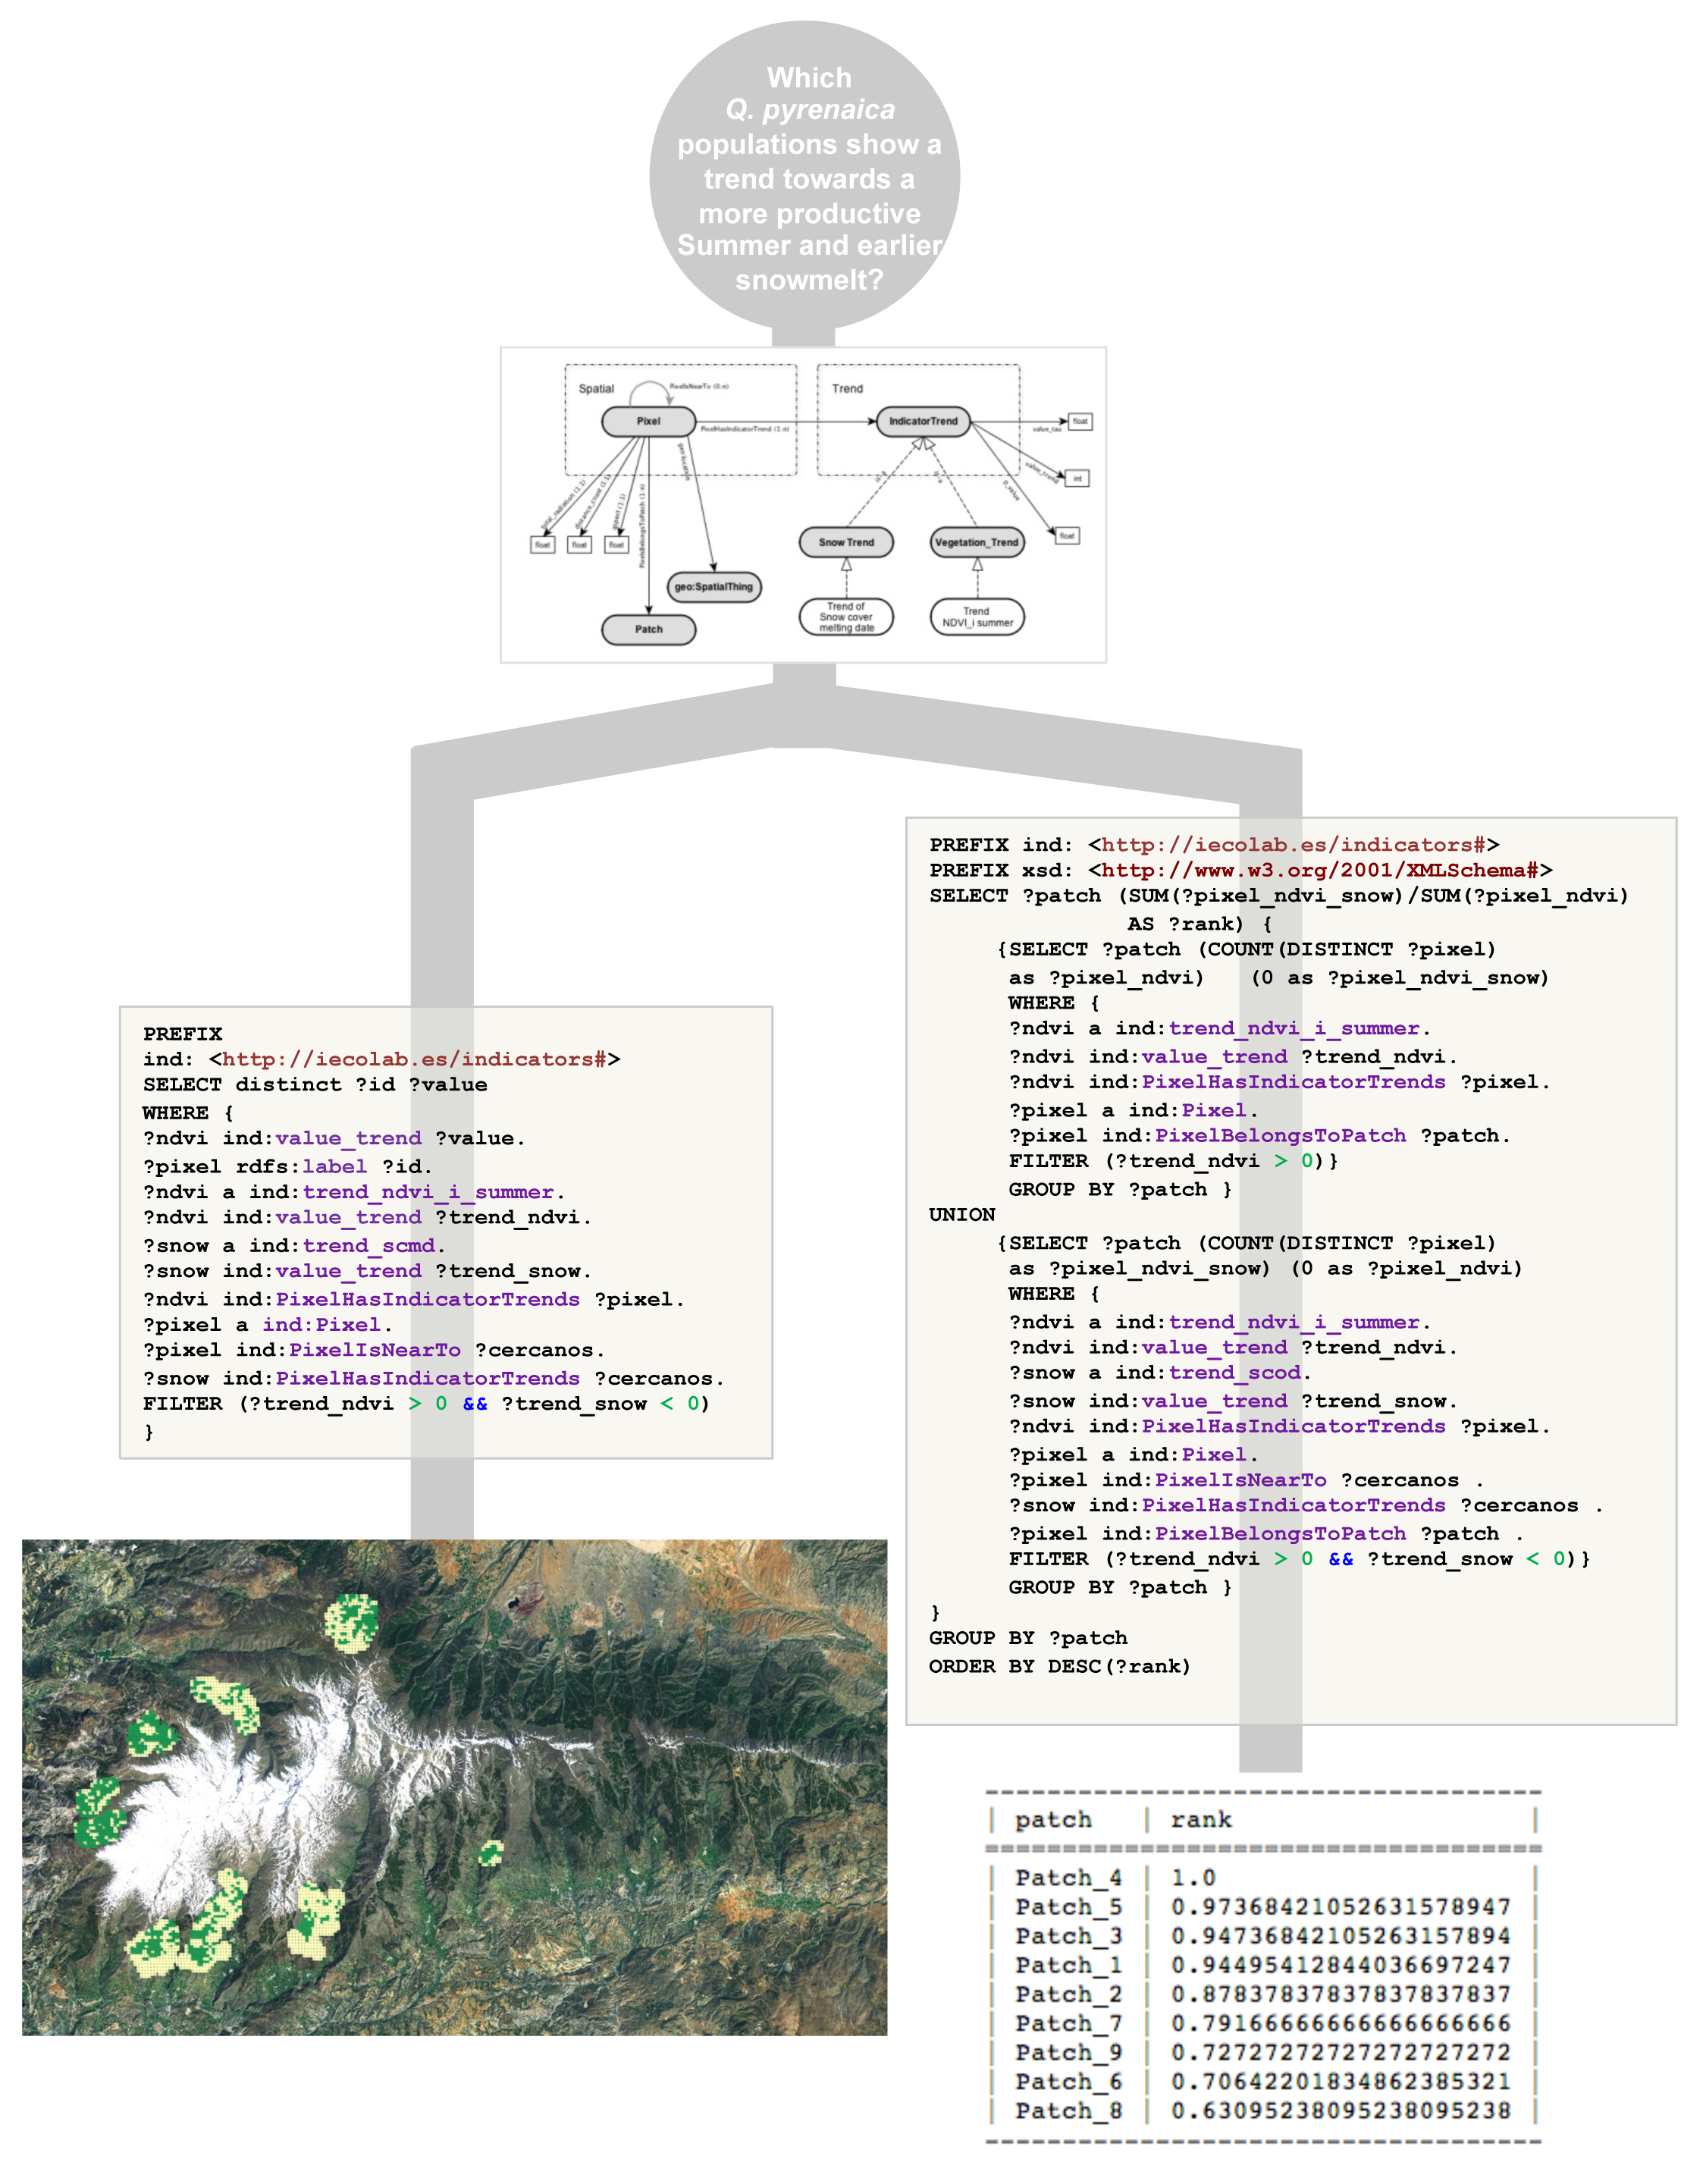
\includegraphics[width=\textwidth]{img/onto/onto-case-studyQ3.jpg}\caption{Scheme showing the process of answering a complex query by the ontology. The question takes into account trends in habitat functioning as well as trends in snow-cover melting date. We first show the concepts used by the ontology to answer the query, then the SPARQL code and finally the results found. The left branch provides a map showing those pixels with trends towards more productive summers and earlier snowmelt date. The right branch offers a table ranking the Pyrenean oak patches according to the percentage of pixels that satisfies both conditions.}\label{fig:onto:casestudyQ3}
\end{figure}
   
% !TEX root = ../my-thesis.tex
%
\selectlanguage{english}  
\chapter{\textcolor{ctcolormain}{Ecosystem services provided by \Qpw oak forests}. A study case from Sierra Nevada mountain range (southern Spain)}\label{sec:es}

\mbox{}
\vfill
%{\color{ctcolormain}\textbf{Antonio J. Pérez-Luque}}; José V. Roces-Díaz \& Regino Zamora (In prep.)


\newpage

\paragraph{Abstract} \mbox{} \\
\Qp forests are relevant part of the Iberian landscape and have suffered intense anthropic pressures causing modifications in their structure and composition. Historically they were exploited in coppice for charcoal, firewood, or they were thinned and even burned to create grazing areas. Recent abandonment of traditional uses and exploitation since the middle of the last century has led to a decrease in anthropic pressure on these ecosystems. Paradoxically, some of these oak woodlands present a state of advanced degradation (stagnation of growth; scarce regeneration; etc), with stands with high densities and high biomass accumulation, increasing the fire risk. Taking into account this situation, and considering the vulnerability of this species to global change, it is necessary to search alternatives to the traditional uses of coppice management, particularly for those stands located in their rear edge, such us the oak woodlands of Sierra Nevada, due to their relevance for the species conservation. In this work we present a comprehensive review of the main ecosystem services (ES) provided by melojo oak forests. Then, using the Sierra Nevada (SN) melojo oak populations as study-case, we explore more in depth the ES provided by these woodlands. We combined expert knowledge and a series of datasets from different sources (\emph{e.g.} grey literature, monitoring programs) to quantify as far as possible the ES provided by these forests. We also explored the spatial pattern of some ES among the melojo oak populations within SN mountain range. Provisioning (\emph{e.g.} use of melojo oak wood in the wine production) and regulating services (\emph{e.g.} carbon sequestration and soil fertility) were widely reported in the literature review meanwhile no studies assessing cultural ES were found in our literature review. However, this pattern changes when the ES were analyzed in more detail as in our study case, highlighting the existence of diverse cultural services provided these forests in Sierra Nevada. The quantification of ES in SN showed differences among the supply of ES by the melojo oak populations, with southern populations have higher values of regulating services and northern ones exhibited higher values for cultural services. Our compilation of local-level data has allowed us to quantify many of ES supplied by the \Qpy forests, which could aid to natural resource managers with more information and tools to help them in the decision-making process.
\newpage

\section{Introduction}\label{sec:es:intro}

Mediterranean forests are subject to significant and simultaneous climatic and anthropogenic pressures {FAOPlanBleu2018StateMediterranean, DoblasMirandaetal2017ReviewCombination}, and climate change is expected to strongly affect to Mediterranean Region \autocite{GiorgiLionello2008ClimateChange, Penuelasetal2017ImpactsGlobal,Crameretal2018ClimateChange,Crameretal2020ClimateEnvironmental}. The impacts of global change on Mediterranean forest ecosystems are altering the supply of ecosystem services \autocite{Lindneretal2010ClimateChange,Lindneretal2014ClimateChange,NoceSantini2018MediterraneanForest,Penuelasetal2017ImpactsGlobal,SerradaHierroetal2011ImpactosVulnerabilidad} particularly in mountainous regions, which have shown a high vulnerability to climate change \autocite{Schroteretal2005EcosystemService}. Notwithstanding, Mediterranean forests provide a wide range of ecosystem services (ES), and represent a great asset and opportunities for the future of the Mediterranean basin \autocite{Gauquelinetal2018MediterraneanForests, NoceSantini2018MediterraneanForest}. Hence, the importance of Mediterranean forests derives both from their current value in terms of area and goods and services, and from the potential role they are likely to play in the future as providers of ES \autocites{FAOPlanBleu2018StateMediterranean}.

Among the Mediterranean type forests, the oak woodlands, \emph{i.e.}, those dominated by oak tree species (\emph{e.g.} \emph{Quercus ilex}, \emph{Q. suber}, \emph{Q. robur}, \emph{Q. faginea}, \emph{Q. petraea}, \emph{Q. pubescens}, \emph{Q. pyrenaica}, \emph{Q. canariensis}) are key ecosystems providing variety of ES \autocite{Maranonetal2020IberianOaks}. For example, their capacity to sequester carbon and therefore to regulate the climate and to mitigate the effects of climatic change is a remarkable regulating service. Oak forests contribute to soil fertility and to the regulation of air, soil and water quality \autocite{Maranonetal2012EstadoTendencia}. These woodlands also provide several raw materials: cork, firewood, acorns \autocite{Bugalhoetal2011MediterraneanCork}. In addition, their role as providers of a wide variety of cultural services, such as recreational, aesthetic and spiritual has been also highlighted \autocite{Lofetal2016ManagementOak}. In order to conserve these forests and their biodiversity, and to manage them in a sustainable way, it is important to be aware of their real and potential supply of ES.

\subsubsection{The case of melojo woodlands (\Qpy) in the Western Mediterranean Region}\label{sec:es:intro-qp}
\Qpw (Pyrenean oak, \emph{melojo}) is a marcescent tree species widely distributed throughout southwestern France and the Iberian Peninsula with some populations at the mountain areas of northern Morocco \autocites{Franco1990Quercus} (FIGURA 1). In the Iberian Peninsula, these forests (in this chapter we will refer to \Qpy forests as \emph{melojo} oaklands or \emph{melojo} woodlands) occupy siliceous soils under meso-supramediterranean and mesotemperate areas and subhumid, humid, and hyperhumid ombroclimate \autocites{delaSernaetal2016MarcescentQuercus,Gavilanetal2018SclerophyllousDeciduous}. The rear-edge populations of this species are restricted to high-mountain areas where they persist as isolated nuclei with ecological conditions very different from those of the main distribution area \autocites{PerezLuqueetal2021EcologicalDiversity}. Sierra Nevada mountains (37°N, 3°W, Spain) represent one of the southernmost European limits for this species (FIGURA 1B). In this mountain area, considered a glacial refuge for deciduous \emph{Quercus} species \autocite{Olaldeetal2002WhiteOaks}, there are eight melojo oak patches, occupying a total of 2400 ha, and ranging from 1100 to 2000 \emph{m.a.s.l.}. Among the forest ecosystems in Sierra Nevada, melojo woodlands are the richest regarding vascular plant species, containing a large number of endemic and endangered plant species \autocite{Loriteetal2008PhytosociologicalReview}, and they also harbor high levels of intraspecific genetic diversity  \autocite{ValbuenaCarabanaGil2013GeneticResilience,ValbuenaCarabanaGil2017CentenaryCoppicing}. 

\Qp woodlands, like other forest ecosystems in Mediterranean area, have been subject to intense anthropogenic pressures over time \autocite{GarciaJimenez20099230Robledales}, resulting in a reduction of their extension and a modification of their floristic composition \autocites{Serradaetal1992CoppiceSystem,Gavilanetal2000EffectsDisturbance,PerezLuqueetal2021EcologicalDiversity} and of their structural patterns \autocites{Calvoetal1999PostfireSuccession,Tarregaetal2006ForestStructure}. Historically, these woodlands have been exploited in coppices for obtaining several products such as firewood, charcoal, tannins, casca (\emph{i.e.} parts of the bark used to extract tannins), and many other traditional uses \autocites{RuizdelaTorre2006FloraMayor,SanchezPalomaresetal2008EstacionesEcologicas}. For instance, after the Spanish Civil war (since 1940's), some oak woodlands were massively cut down to use the firewood as fuel for automobiles (\emph{e.g.} Dehesa de San Jerónimo, Sierra Nevada)\autocite{Prieto1975BosquesSierra}. Forest management for coppices consisted of clear-cutting in rotation periods of 12-20 years, causing the profusion of shoots from the stool highly appreciated by livestock \autocite{Bravoetal2008SelviculturaMontes}. Thinning  and sometimes even burned have also been carried out to create pastures with low densities of mature trees that provide acorns, firewood and large areas for grazing \autocites{HerreraCalvo2016UsoPastoral,Alvarezetal2009CambiosEstructura,ValbuenaCarabanaGil2017CentenaryCoppicing}. In fact, overgrazing in these formations have caused strong soil erosion loss, which was noticed by forest managers since the end of the 19th century \autocites{Laguna1872ComisionFlora}. In some areas, the strong anthropic pressure provoked the loss of the forest cover. For instance, in southern slopes of Sierra Nevada mountains, oak woodlands were almost completely removed at the beginning of the 20th century, which led to some of its watershed being considered among the most torrential in Spain  \autocites{RomeroZurbano1909DivisionHidrologicoforestal}. All these anthropogenic processes have transformed the melojo woodlands in a deep way that it is difficult to find stands that can be considered natural forests  \autocites{RuizdelaTorre2006FloraMayor}. 

However, the abandonment of livestock and forestry traditional uses since the middle of the last century due to rural abandonment  \autocites{MacDonaldetal2000AgriculturalAbandonment}, has caused a decrease in anthropogenic pressure on Mediterranean forest  \autocites{ValbuenaCarabanaetal2010HistoricalRecent}, being particularly important for mountain areas \autocites{JimenezOlivenciaetal2015MedioSiglo,JimenezOlivenciaetal2015EvolucionUsos,Piasetal2014ColonizationAbandoned}. Paradoxically, and considering this decrease in anthropogenic pressure, many of the oak stands present a state of advanced degradation, showing growth stagnation, lack of fruiting, and also sings of branch dieback \autocites{Canellasetal2004GrowthResponse, Bravoetal2008SelviculturaMontes, ValbuenaCarabanaGil2014EfectosGestion, PiqueVericat2015EvolutionPerspectives, Piqueetal2018Spain}. Many stands, derived from the high resprout capacity of \Qp, also have high tree density that would increase the vulnerability to drought of these stands, as has been reported in other forests across world  \autocite{McDowelletal2020PervasiveShifts}. The high tree density together with the accumulation of biomass and high horizontal continuity, would increase the risk of fire \autocites{Bravoetal2008SelviculturaMontes,GarciaJimenez20099230Robledales}. In addition, these problems may be aggravated in the current context of climate change (increase in temperatures and higher incidence of extreme events such as droughts)  \autocites{IPCC2013ClimateChange,Spinonietal2018WillDrought}, particularly considering the high vulnerability of this species to climate change \autocites{Benitoetal2011SimulatingPotential,GarciaValdesetal2013ChasingMoving,SanchezdeDiosetal2009PresentFuture,GeaIzquierdoetal2013GrowthProjections}, and especially for areas located in the rear edge of their distribution range such us Sierra Nevada mountain range.  

In view of this current situation of vulnerable (to global change drivers) forest stands, affected by the progressive abandonment of traditional land uses during the last decades, the need of defining alternative uses for melojo oak woodlands has been point out \autocites{MesonMontoya1985VegetacionForestal,SanMigueletal2012BosquesMatorrales}, and some management alternatives have been proposed \autocite[\emph{e.g.} sylvopastoral uses, see][]{HerreraCalvo2016UsoPastoral}. In this sense, the identification and characterization of the main ES becomes a crucial to develop landscape planning and forest management strategies in a global change context \autocites{Piqueetal2018Spain}. 

Despite the wide variety of ES provided by oaklands is worldwide acknowledged, very little has been written specifically about the provision of ES by oak-dominated forests  \autocites{Maranonetal2012OakTrees,Maranonetal2012EstadoTendencia,MorenoLlorcaetal2012MontanaMediterranea}. Some works have carried out a general valuation of the ES provided by the different \emph{Quercus} woodlands at regional and national scales \autocite{SanMigueletal2012BosquesMatorrales,Maranonetal2012EstadoTendencia,Sousaetal2020EcosystemServices}, and some studies provided temporal trend analysis of ES from an economic perspective \autocites[see][for an example for dehesas of California and Spain]{Caparrosetal2013EconomicsEcosystem}. However, to our knowledge, there is no comprehensive review of the ES provided by \Qp woodlands. 

The aim of this work is to carry out a review of the main ES provided by Q. pyrenaica woodlands. Firstly, we conducted a literature review to know the general state of the art and to summarize some of the most relevant ES provided by these formations. Secondly, using the Sierra Nevada oak populations as study-case we explore more in depth the ES provided by these woodlands. For this purpose, we combined expert knowledge and a wide variety of data coming from ecological monitoring programs and several research projects to quantify as far as possible the ES provided by these forests. We are also interested in exploring how the ES are spatially distributed in this mountain region. For this, we searched for differences on the supply of ES between the melojo oak populations within Sierra Nevada mountain range.  

\section{Material and methods}\label{sec:es:mat}
\subsubsection{Study area}\label{sec:es:mat-studyarea}
Sierra Nevada is a mountainous region located in the south-eastern Iberian Peninsula (37º14'-36º54'N; 2º37'-3º39'W) covering more than 2000 km\textsuperscript{2} with an elevation range of between 860 and 3482 \emph{m.a.s.l.} The climate is Mediterranean, characterized by cold winters and hot summers, with a pronounced summer drought. The annual average temperature decreases in altitude from 12-16 ºC below 1500 \emph{m.a.s.l.} to 0 ºC above 3000 \emph{m.a.s.l.}. Annual precipitation ranges from less than 250 mm in the lowest areas of the mountain range to more than 700 mm in the highest peaks. Winter precipitation is mainly in the form of snow above 2000 \emph{m.a.s.l.}. Topographically, the area is heterogeneous, with strong climatic contrasts between the sunny, dry south-facing slopes and the shaded, wetter north-facing slopes. This mountain range is considered one of the most important biodiversity hotspots in the Mediterranean region \autocite{Blancaetal1998ThreatenedVascular}, hosting 105 endemic plant species for a total of 2353 taxa of vascular plants (33\% and 20\% of Spanish and European flora, respectively) \autocite{Lorite2016UpdatedChecklist}. Forest cover in Sierra Nevada is dominated by pine plantations (\emph{Pinus halepensis} Mill., \emph{Pinus pinaster} Ait., \emph{Pinus nigra} Arnold subsp. \emph{salzmannii} (Dunal) Franco, and \emph{Pinus sylvestris} L.) covering approximately 37000 ha. Native forests are mainly dominated by holm oak (\emph{Quercus ilex} subsp. \emph{ballota} (Desf.) Samp.) occupying low and medium mountain areas, and melojo oak ranging from 1100 to 2000 \emph{m.a.s.l.} \autocite{PerezLuqueetal2019MapEcosystems}.

\subsubsection{Selection of ecosystem services and their assessment }\label{sec:es:mat-selection}

In order to analyze the ES provided by melojo forests, we have carried out two different phases. Firstly, performed a general literature review to explore the state of the art on the ES provided by these forests. Secondly, taking into account the results of the general literature review, we have carried out a more comprehensive analysis of the ES provided by the melojo forests in Sierra Nevada. We have characterized their supply for Sierra Nevada mountain region, and where data were available, we have quantified them, and compared between melojo populations identified Sierra Nevada. For the classification and definition of ecosystem services, we adapted the CICES V5.1 (Common International Classification of Ecosystem Services) approach \autocites{HainesYoungPotschin2018CommonInternational}. We have considered three categories of ecosystem services: provisioning, regulating and cultural, and for each of them, we have identified different ES indicators. Due to the large number of ES studied, we have considered it more practical to explain for each of the ES, the indicator(s) used to quantify it (see details in the following section).  

To characterize the scientific literature that evaluate the ES of the melojo oak woodlands, we performed initially a systematic search in the ISI Web of Knowledge (search date: October 2020). We compiled references published in indexed journals included in the Journal of Citation Reports (JCR), in English language, since 1970 to 2020, that evaluated a wide variety of ES indicators in these woodlands. First, we conducted a search for papers on the study species with the term \emph{"Quercus pyrenaica"} in the title, keywords or abstract, which produced 393 results. We applied a second criterion, to extract papers that analyzed possible services, including a broad list of terms (also in the title, keywords or abstract) related to ES
(TABLE S1 \tabref{tab:es:wos}). The combination of both produced 188 results. After reviewing their abstracts, we selected 60 papers that met the premise of evaluating ES in melojo oak woodlands (TABLE S2 \tabref{tab:es-review}). We omitted papers focused exclusively on descriptive aspects of these ecosystems (\emph{e.g.} floristic composition or ecosystem structure), their biodiversity (\emph{e.g.} species richness) which were not directly related to ecosystem service indicators. 

For each of the ES reviewed, we initially described the general status of the services in these woodlands using the compiled references. Then, we performed a quantification for the Sierra Nevada oak woodland populations, as long as data were available. The values for the quantification were obtained both from the literature review and from several research datasets in combination with the expert criterion (Table 1, (\tabref{tab:es:data}). ). For those ES with data availability, we performed a quantification for each of the oak population clusters identified in Sierra Nevada, i.e. Northern (N), Northwestern (NW), and Southern (S) \autocite[ see][]{PerezLuqueetal2021EcologicalDiversity}. We compared differences in the supply of ES between the oak population clusters.

\begin{table}[]
\caption{Search terms used in the literature review.}
\label{tab:es:wos}
\footnotesize
\begin{tabular}{>{\centering}p{11cm}l}
\toprule
\textbf{TOPIC (i.e. Title OR Keywords OR Abstract)} & \textbf{Results} \\ 
\toprule
\emph{"Quercus pyrenaica"} & 393 \\ \midrule
\emph{"ecosystem service*" OR "ecologic* process*" OR "ecologic*
function*" OR "provision*" OR "regulat*" OR "cultural" OR ``support*'' OR
"food" OR "mushroom*" OR "fruit*" OR "berry" OR "berries" OR
``cattle'' OR ``stock'' OR ``livestock'' OR ``sheep*'' OR ``goat*'' OR
``game'' OR ``hunt*'' OR ``wine'' OR "fresh water" OR "water supply" OR "drink* water" OR ``water
yield*'' OR ``firewood'' OR ``wood'' OR ``timber'' OR ``coal'' OR "climat* regulat*" OR "carbon sequest*" OR "carbon stock*" OR "carbon stor*" OR "soil fertilit*" OR "soil nutri*" OR "nutri* cycle*" OR "soil
carbon*" OR "organic carbon" OR "water regulat*" OR "soil water" OR "water cycle" OR "water stor*"
OR "water qualit*" OR "water depurat*" OR "water filtrat*" OR "water
clean*" OR ``snow regulat*'' OR ``snow storage'' OR "soil erosion" OR "soil protection" OR "erosion protection" OR
"erosion control" OR "soil loss" OR "water erosion" OR "landscape qualit*" OR "aesthetic*" OR "landscape value*" OR
"recreation*" OR "social percept*" OR ``spiritual value'' OR
``scientific knowledge''} & 188 \\
\bottomrule
\end{tabular}
\end{table}

\begin{sidewaystable} 
\caption{Ecosystem Services (ES) indicators used in this study. For each indicator the ES category, references, units, and data source are indicated. (\emph{R}): regulation; (\emph{S}): provisioning and supporting; (\emph{C}): cultural. (*) extracted from the literature; (**) own calculations. (+) indicators with data for oak populations of Sierra Nevada.}\label{tab:es:data}
\centering
\scriptsize
\begin{adjustbox}{width=\linewidth}
\begin{threeparttable}
\begin{tabular}{>{\raggedleft}m{0.087\linewidth}>{\centering}m{0.108\linewidth}m{0.4\linewidth}>{\centering}m{0.102\linewidth}m{0.165\linewidth}m{0.071\linewidth}}
\textbf{Ecosystem Service} & \textbf{ES indicator used} & \textbf{Bibliographic References} & \textbf{Units} & \textbf{Data Source} & \textbf{Data for Sierra Nevada } \\ \toprule 
Experiential use of Landscape (C) & Number of photographies (*) & \autocite{MorenoLlorcaetal2020EvaluatingTourist} & Number of photographies & \autocite{RosCandeiraetal2020SocialMedia} & Yes (+) \\
Physical use of Landscape (C) & Wikiloc tracks (**) &  & Routes density; Total routes & Wikiloc & Yes (+) \\
Recreational (C) & Visitors numbers (**) &  & Visitor numbers & Sierra Nevada Natural and National Protected Area & Yes (+) \\
Scientific (C) & Research requests permisision (**) & \autocite{Zamoraetal2016GlobalChange} & Number of Research requests & Sierra Nevada Natural and National Protected Area & Yes (+) \\
Scientific (C) & Density of socio-ecological monitoring methodologies (**) & \autocite{Zamoraetal2016GlobalChange} & Density of monitoring methdologies & Sierra Nevada Natural and National Protected Area & Yes (+) \\
Symbolic (C) & Singular trees (*) & \autocites{IruritaFernandezetal2003ArbolesArboledas, SanchezGarciaetal2003ArbolesArboledas} &  & Andalusia Regional Goverment & Yes \\
Biodiversity (S) & Bird richness (**) & \autocites{BareaAzconetal2012PasseriformesOtras,PerezLuqueetal2016DatasetPasserine,ZamoraBareaAzcon2015LongTermChanges,PerezLuqueetal2021ManualGestion} & Species number & Sierra Nevada Global Change Observatory & Yes (+) \\
Biodiversity (S) & Fungal diversity (*) & \autocites{Ortegaetal2010MycorrhizalMacrofungi, MorenoArroyo2004InventarioMicologico} & Species number & Basic Mycological Inventory of Andalusia &  \\
Biodiversity (S) & Genetic diversity (*) & \autocites{ValbuenaCarabanaGil2013GeneticResilience,ValbuenaCarabanaGil2013ReduceAprovechamiento,ValbuenaCarabanaGil2014EfectosGestion,ValbuenaCarabanaGil2017CentenaryCoppicing} &  &  & Yes (+) \\
Biodiversity (S) & Microbial diversity (*) & \autocites{CoboDiazetal2017TaxonomicFunctional,Lasaetal2019BacteriaEndosphere, Lasaetal2019MetabarcodingReveals} &  &  & Yes \\
Biodiversity (S) & Woody richness (*) & \autocite{PerezLuqueetal2014SinfonevadaDataset,Loriteetal2008PhytosociologicalReview} & Species number &  & Yes (+) \\
Food provision (S) & Wild mushrooms production (*) & \citet{RayaLopezetal2017MuestreosPara} & kg Fungi ha$^{-1}$ year$^{-1}$ & Plan CUSSTA (Plan for the Sustainable Use and Conservation of Mushrooms and Truffles in Andalusia) & Yes \\
Tanning (S) & Percentage of tannins (*) & \autocites{FernandezdeSimonetal2006ChemicalCharacterization,Doceetal2007EffectImmature,TornerOchoa1952CurtientesVegetales} & \% of tannis present at bark &  & \\ 
Timber (S) & Biomass increment & \autocite{PerezLuqueetal2021CarbonSequestration} & Mg ha$^{-1}$ year$^{-1}$ & Spanish National Forest Inventory & Yes \\
Wine Ageing (S) & Phenological compunds (*) & \autocites{Ramiloetal2017VolatileOrganic,Gallegoetal2012PhenolicCompounds, CadahiaFernandezdeSimon2004UtilizacionRoble,FernandezdeSimonetal2008VolatileCompounds,FernandezdeSimonetal2009VolatileCompounds, Gallego2013EstudioPotencial,MartinezGiletal2020EffectSize} &  &  &  \\
Climate Regulation (R) & Carbon sink (**) & \citet{PerezLuqueetal2021CarbonSequestration} & Mg CO$_2$ ha$^{-1}$ & LIDAR and Forest Inventories & Yes (+) \\
Climate Regulation (R) & Vegetation Index (NDVI, EVI) (*) & \autocites{Dionisioetal2012SatelliteBasedMonitoring,AlcarazSeguraetal2016ChangesVegetation,PerezLuqueetal2015OntologicalSystem,Cazorlaetal2020RemoteSensingbased} &  & MODIS & Yes (+) \\
Climate Regulation (R) & Regulation of temperature (**) & \autocite{Zamoraetal2021UniendoMacro} &  & ClimaNevada & Yes \\
Control of erosion (R) & Soil erosion Control (*) & \autocites{MesonMontoya1985VegetacionForestal,Salomonetal2017GeneralFailure} &  &  &  \\
Soil Fertility Regulation (R) & Soil Organic Carbon (**) & \citet{Hengletal2017SoilGrids250mGlobal, Batjesetal2017WoSISProviding, Batjesetal2020StandardisedSoil} & Mg SOC ha$^{-1}$ & SoilGrid database & Yes (+) \\
\bottomrule
\end{tabular}
\end{threeparttable}
\end{adjustbox}
\end{sidewaystable}

\section{Ecosystem Services provided by \Qp woodlands}\label{sec:es:results}
The compilation of literature carried out has shown us those services that have been most frequently evaluated in works focused on \Qp woodlands (see \tabref{tab:es:wos}). Of the 60 papers selected in the literature review, provisioning services were the most frequently evaluated. Among them, the studies focused on investigating the effect of melojo wood in the wine production process stand out (\emph{n} = 26/60) \autocites[\emph{e.g.}][]{FernandezdeSimonetal2010CharacterizationVolatile,CastroVazquezetal2013EvaluationPortuguese}, since barrels are frequently built with the wood of this species. In addition, we found different studies evaluating mushroom production \autocites[\emph{e.g.}][]{OriadeRuedaetal2010CouldArtificial}, the effect of this species on livestock production \autocites[\emph{e.g.}][]{Nunezetal2012LivestockManagement}, or the production of wood or biomass for energy (\emph{n} = 6/60) \autocites[\emph{e.g.}][]{Mirandaetal2009EnergeticCharacterization}. Regarding regulation services, several studies evaluate the role of forests in soil quality and fertility (\emph{n} = 12/60), or their capacity for carbon sequestration and storage \autocites[\emph{n} = 12/60; \emph{e.g.}][]{Alvarezetal2014InfluenceTree}. There also a high proportion of studies on soil carbon \autocites[\emph{n} = 8/60; \emph{e.g.}][]{Fonsecaetal2019ImpactTree}. Finally, it should be noted that, applying the above-mentioned search criteria, no studies on the evaluation of cultural services in the \Qpy woodlands have been found.

POR AQUI VAS ---- 
\subsection{Regulating services}\label{sec:es:regulation}
\subsubsection{Soil climate regulation}\label{sec:es:regulation-soil}
The cover provided by woodlands is key to regulating soil temperature \autocite{Ellisonetal2017TreesForests}. Soil temperature is one of the main factors affecting seed germination, plant growth and development, being as important as air temperature, since it can limit root formation \autocites{AlvarezUriaKorner2007LowTemperature}. The marcescent feature of \Qp allows the accumulation of leaf litter layer on the ground during a part of the year. This accumulation can have positive effects on seedling establishment because it acts as a thermal insulator \autocites{Loydietal2014DistributionEffects}, helping to alleviate the damage effects of freezing on seeds \autocites{Loydietal2014DistributionEffects,CavenderBaresetal2005SummerWinter,EstesoMartinezGilPelegrin2004FrostResistance,Lofetal2019TammReview}. This buffer effect can also be important once germination starts, since negative temperatures can suspend the process and damage the radicle and epicotyl \autocites{AizenWoodcock1996EffectsAcorn}. However, negative effects on seed germination and establishment could prevail (\emph{e.g.}, pathogen proliferation; allelopathic effects) when litter accumulation exceeds a certain threshold \autocites{Loydietal2014DistributionEffects,XiongNilsson1999EffectsPlant}.

It has also been noticed the importance of the forest cover on the regulation of extremes temperatures registered during the summer period \autocites{DeFrenneetal2021ForestMicroclimates}. It is particularly important for melojo oaks woodland located at the warm rear-edge of their distribution. For instance, using microclimatic data from a sensor network deployed in an oak woodland located at southern slopes of Sierra Nevada, \citet{Zamoraetal2021UniendoMacro} found strong variations of the air and soil temperatures registered inside the \Qp forest compared with the registered on forest's open areas (\figref{fig:es:temp}). The soil temperatures varied up to 15ºC between microhabitats on a day of maximum temperatures during the summer period. This highlights the role of the oak tree vegetation on the regulation of the thermal environment \autocites{Niinemets2010ResponsesForest}. The oak forest cover provides a cooler environment, reducing potential evapotranspiration and alleviating the water stress to which these formations are subjected in summer \autocites{Zamoraetal2021UniendoMacro}.  

\begin{figure}[H]
    \centering
    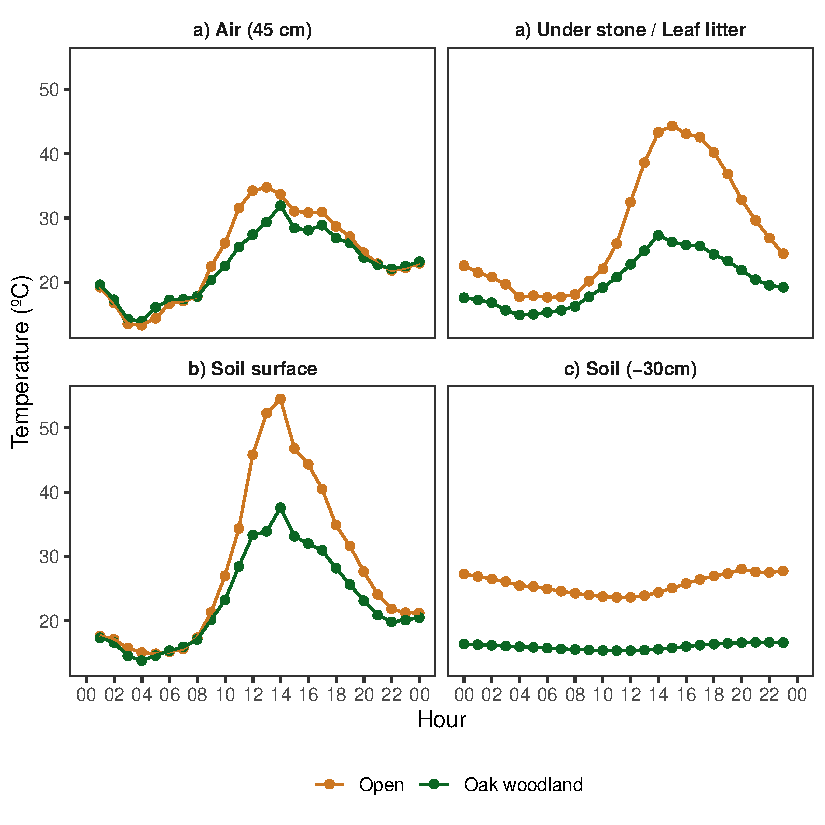
\includegraphics[width=\textwidth]{img/es/es-profiletemp.pdf}\caption{Hourly variation of the temperature on July 19, 2018 (hottest day of the 2018-2019 period in the "Robledal de Cáñar" oak woodland. \textbf{a)}. Variation in air temperature recorded at 45 cm in forest areas (green line) and in forest clearings (brown line). \textbf{b)}. Variation of the temperature for the covered soil (under stone; or under litter); anf of the temperature of the soil surface (\textbf{c}); and soil temperature at 30 cm depth (\textbf{c}). For each variable, the values recorded in the different habitats are compared: forest clearings (open) and forest areas (forest). Source: \autocite{Zamoraetal2021UniendoMacro}}\label{fig:es:temp}
\end{figure}

\subsubsection{Carbon sequestration}\label{sec:es:regulation-carbon}
Carbon sequestration is one of the most relevant ecosystem services provided by Mediterranean forests \autocites{Gauquelinetal2018MediterraneanForests,NoceSantini2018MediterraneanForest}. The carbon stock can be assumed as an indicator of the capacity of ecosystems to contribute to climate regulation due to their potential to influence the concentration of atmospheric CO$_2$ \autocites{Lauterbach2007AssessmentExisting,Luyssaertetal2008OldgrowthForests}. Mediterranean forests represent a carbon sink that is expected to increase in the coming decades \autocites{Canellasetal2017CarbonSequestration,PasalodosTatoetal2017EvaluationTree}, although recent studies have shown a ralentization of this increase \autocites[][]{RocesDiazetal2021TemporalChanges}.

Recently, a cartography of the biomass and carbon sequestration potential of \Qp woodlands of Sierra Nevada were generated \autocites{PerezLuqueetal2021CarbonSequestration} (see also chapter \ref{sec:carbon}). These authors, combining information from LIDAR (\emph{Light Detection And Ranging}) remote sensing with information from different forest inventories, estimated a total biomass (aboveground- and belowground-biomass) of 9.94 Tg (1 Tg = 10$^12$ g) in the \Qp forests of the Sierra Nevada, which represents a potential CO$_2$ sequestration of 17.33 Tg (1 Tg = 10$^12$ g). This highlights the importance of these forests in carbon sequestration, which represents a key ecosystem regulating service.

Spectral vegetation indices, \emph{e.g.} EVI and NDVI are frequently used to derive indicators of ecosystem functioning, such as the total annual carbon absorbed by vegetation, or the seasonality and phenology of carbon gain dynamics \autocites{Xiaoetal2019RemoteSensing,
AlcarazSeguraetal2009BaselineCharacterization,AlcarazSeguraetal2009UseDescriptors,Cazorlaetal2020RemoteSensingbased}. Some works have analyzed the evolution of the productivity of different ecosystems in Sierra Nevada using vegetation indices from MODIS satellite data \autocites{Dionisioetal2012SatelliteBasedMonitoring,AlcarazSeguraetal2016ChangesVegetation,PerezLuqueetal2015OntologicalSystem,Cazorlaetal2020RemoteSensingbased}. The results of these works have revealed that melojo oak forests, despite their high seasonality, are the most productive ecosystems in Sierra Nevada for the period analyzed (2000-2017), highlighting their importance in carbon gain and therefore as carbon sinks. Likewise, the time series analysis showed a positive trend in productivity (EVI) for most Sierra Nevada oak forests, possibly related to the increase in temperature \autocite{PerezLuqueetal2015OntologicalSystem}.

Soil organic carbon (\emph{SOC}), the main component of soil organic matter, is considered relevant for many soil processes. For example, SOC content correlates positively with soil fertility, playing a key role determining the physical, chemical and biological qualities of a soil \autocites{Victoriaetal2012BenefitsSoil}. There are different ecosystem services in which SOC is involved, among which regulation and provisioning services stand out \autocites{Francavigliaetal2018OrganicCarbon}. Despite, there are some studies that reported the amount of soil organic carbon in specific locations of the Sierra Nevada oak woodlands \autocites{CoboDiazetal2017TaxonomicFunctional,Lasaetal2019BacteriaEndosphere}, they prove insufficient to provide an approximated estimate of the total SOC content for those oak woodlands. There are, however, soil databases that providing estimates of the SOC content at a ecosystem level, such as the SoilGrid database (https://soilgrids.org/), which provides digital maps of different soil variables at a 250-m spatial resolution \autocites{Hengletal2017SoilGrids250mGlobal,Batjesetal2017WoSISProviding,Batjesetal2020StandardisedSoil}. For Sierra Nevada, those maps reported an average SOC content (mean SOC at 0-30 cm depth) of 51.8 Mg ha$^-1$ (20-80 Mg ha$^-1$) (\figref{fig:es:soc}), while the oak forests have a average SOC value of 53.5 Mg ha$^-1$ (45-67 Mg ha$^-1$), with southern oaks populations showing significantly higher values. 

\begin{figure}
    \centering
    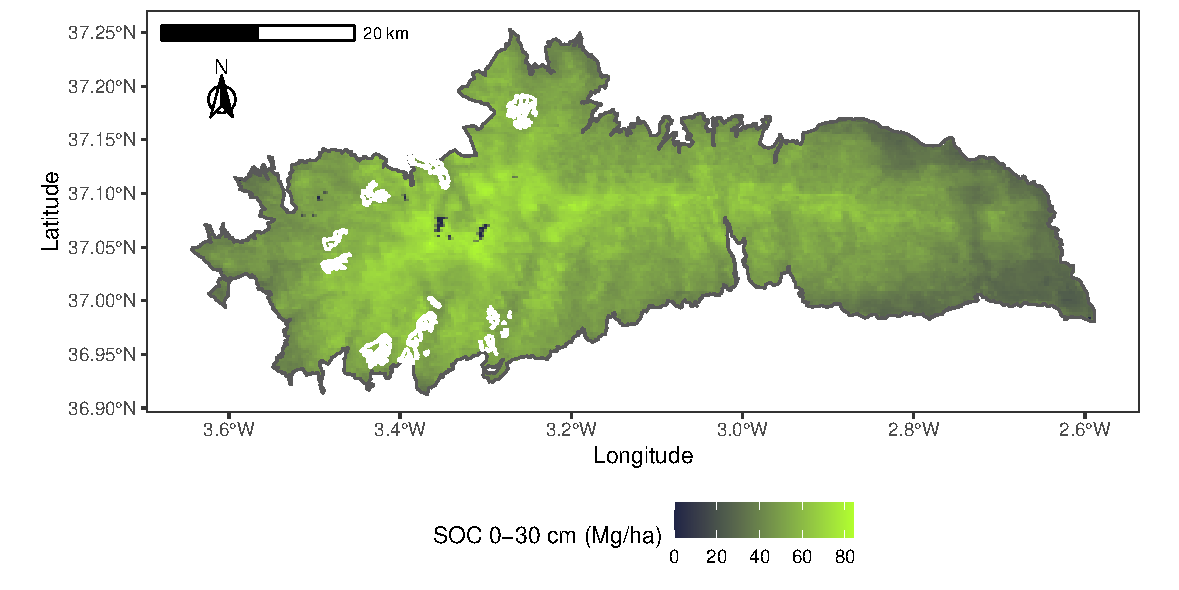
\includegraphics[width=\textwidth]{img/es/es-soc.pdf}\caption{Distribution of the Soil organic carbon in Sierra Nevada. Oak populations in white. Drawn with data from SoilGrid database \autocites[see][]{Hengletal2017SoilGrids250mGlobal}}\label{fig:es:soc}
\end{figure}

\subsubsection{Erosion control}\label{sec:es:regulation-erosion}
Forests have a key role in the reduction of the erosive rainfall impact on soil, so they provide an important regulating service \autocites{Zhongmingetal2010StratifiedVegetation,GarciaRuizetal2011MediterraneanWater}. The root system of \Qp consists of two well-differentiated types \autocites{Allue1995OrdenacionMasas}: \emph{(i)} the main root, characteristic of the genus, which allows for powerful anchoring to the soil; and \emph{(ii)} a layer of roots close to the soil surface and parallel to it, which could emit large number of shoots that form a dense network. Those root systems that help to maintain soil integrity by preserving landslides \autocites{MesonMontoya1985VegetacionForestal,Salomonetal2017GeneralFailure} (\figref{fig:es:roots}). In addition, the extraordinary regrowth capacity of \Qp, both of stump and roots, gives it functional advantages over other species, such as its response to disturbances (\emph{e.g.}, fires), particularly on sloping areas \autocites{RuizdelaTorre2006FloraMayor,ValbuenaCarabanaGil2017CentenaryCoppicing}. The profusion of resprouts provides an important ecosystem service of regulation, since the resprouts effectively maintain the soil in mountainous areas, reducing the impact of erosive processes and the soil loss  \autocites{MesonGarcia1984BasesEcologicas}.

\begin{figure}
    \centering
    \includegraphics[width=\textwidth]{img/es/es-roots.jpg}\caption{Structure of the complex root system of several specimens of \Qp. Picture from R. Salomón.}\label{fig:es:roots}
\end{figure}

\subsection{Supporting and provisioning services}\label{sec:es:provision}
\subsubsection{Biodiversity}\label{sec:es:provision-biodiversity}

\Qp forests in Sierra Nevada have high values of phytosociological uniqueness \autocites{Loriteetal2008PhytosociologicalReview}, which could be explained because they act as habitat providers for other relict species. In fact, the role of refugee of Sierra Nevada for this oak ecosystem \autocites{Breweretal2002SpreadDeciduous,Olaldeetal2002WhiteOaks,RodriguezSanchezetal2010TreeRange}, translates into a great diversity of plant species, being the forest formation with the greatest richness in Sierra Nevada, although it only represents 7\% of the forest area \autocites{PerezLuqueetal2014SinfonevadaDataset}. A key role of \Qp woodlands in Sierra Nevada is that they provides optimal conditions for the presence of several plant species cataloged under different threatened categories \autocites{Lorite2016UpdatedChecklist,Losaetal1986PaisajeVegetal,MelendoValle2000EstudioComparativo}, such as the hybrid mustard (\emph{Sorbus hybrida} L.) considered \emph{critically endangered} (CR), the \emph{endangered} (EN) goat willow (\emph{Salix caprea} L.), the holly (\emph{Ilex aquifolium} L.) and the yew (\emph{Taxus baccata} L.) considered \emph{vulnerable} (VU), and others with a lower level of threat (\emph{e.g.} \emph{near threat}, NT) (\emph{e.g.} the rowan, \emph{Sorbus aria} (L.) Crantz; or the maple \emph{Acer opalus} subsp. \emph{granatense} (Boiss.) Font Quer \& Rothm.). Many of these species are also considered relict species that find favorable microclimatic conditions in the melojo oak woodlands of Sierra Nevada, which make these ecosystems a refuge for those species \autocites{Blancaetal1998ThreatenedVascular,Lorite2016UpdatedChecklist,Losaetal1986PaisajeVegetal}. 

Birds community of \Qp forests of Sierra Nevada have been studied since 1980's \autocites{ZamoraCamacho1984EvolucionEstacional,ZamoraBareaAzcon2015LongTermChanges,BareaAzconetal2012PasseriformesOtras}. A total of 73 species of passerine bird species has been recorded within these oak forests \autocites{PerezLuqueetal2016DatasetPasserine}. Recent analysis shown differences in diversity between Sierra Nevada oak populations, with lower diversity values for southern oak populations than for northern-ones \autocites{PerezLuqueetal2021ManualGestion}. No differences was found for bird abundance, but a general decrease of several key species (\emph{Garrulus glandarius}) were recorded since 1980 \autocites{ZamoraBareaAzcon2015LongTermChanges}. 

Regarding the fungal community associated with this oak ecosystem, although there are no studies analyzing the composition for oak populations of Sierra Nevada, several works have shown the richness associated to this ecosystem at regional and national scales. Thus, an exhaustive review of the diversity of mycorrhizae-forming macromycetes in the \emph{Quercus} forests of the Iberian Peninsula recorded 174 fungi species in \Qp formations \autocites{Ortegaetal2010MycorrhizalMacrofungi}, of which 5 are included in the Red List of Fungi to be Protected in the Iberian Peninsula. At regional level, the Basic Mycological Inventory of Andalusia (IMBA, \emph{Inventario Micológico Básico de Andalucía}), reported 214 records belonging to 149 fungi taxa, inhabit in \Qp ecosystem \autocites{MorenoArroyo2004InventarioMicologico}. 

Another aspect to consider when analysing the biodiversity of the oak woodlands, is the presence of species using this trees. For instance, \emph{Quercus} species are key in the development of the biological cycle of some insects, such us the oak gall wasp (Hymenoptera: Cynipidae). The galls support species-rich, closed communities of inquilines and parasitoids that have become a model system in community ecology \autocites{Stoneetal2002PopulationBiology}. For instance, in melojo forests of Sierra Nevada have been recorded 30 species of cynipids (representing 21\% of the Iberian species) \autocites{NievesAldrey2013AvispasAgallas}. 

Several studies have analyzed the microbial diversity in the soils of some oak forests in the Sierra Nevada highlighting that the microbial community of this formation is dominated by a few very abundant taxa \autocites{CoboDiazetal2017TaxonomicFunctional,Lasaetal2019BacteriaEndosphere, Lasaetal2019MetabarcodingReveals}. Finally, in relation to the genetic diversity, it has been traditionally assumed that continued coppicing of \Qp over centuries has led to a decline in the genetic diversity of the species, as a result of the strong inter-stem competition and the propagation of a limited number of genotypes 
\autocites{SanchezPalomaresetal2008EstacionesEcologicas,Bravoetal2008SelviculturaMontes}. However, several studies have pointed out the high diversity that these formations harbour \autocites{ValbuenaCarabanaGil2013GeneticResilience,ValbuenaCarabanaGil2013ReduceAprovechamiento,ValbuenaCarabanaGil2014EfectosGestion,ValbuenaCarabanaGil2017CentenaryCoppicing}. The high genetic diversity observed for the Sierra Nevada oak populations, highlights the importance of conserving the populations of this species which in this mountainous region are at the southern limit of their distribution, acting as a reservoir of genetic diversity. 

\subsubsection{Wine aging and tanning}\label{sec:es:provision-wine}
One of the characteristics of oak trees is their ability to emit volatile organic compounds (\emph{VOCs}), which in addition to giving the wines their characteristic flavor, act as an attractant for different insects. More than 50 volatile organic compounds belonging to 12 different chemical classes have been characterized in melojo oak \autocites{Ramiloetal2017VolatileOrganic}. The phenolic compounds produced by \Qp have similar chemical composition to those produced by the main oaks used in wine aging, such as American oak (\emph{Q. alba}) or French oak (\emph{Q. petraea}) \autocites{Gallegoetal2012PhenolicCompounds}. In fact, the results of comparative analysis between wines aged in barrels from these three oak species, have indicated that the wine aged in melojo oak presents oenological features similar to those of the other oaks, being also very positively valued by the wine tasters \autocites{CadahiaFernandezdeSimon2004UtilizacionRoble,FernandezdeSimonetal2008VolatileCompounds,FernandezdeSimonetal2009VolatileCompounds}. All these results highlight the potential use of wood and its derivatives from \Qp for wine aging, which had not been previously used in cooperage \autocites{Gallego2013EstudioPotencial,MartinezGiletal2020EffectSize} (\figref{fig:es:barrica}). 

The bark and leaves of the \Qp contain a great diversity and a high percentage of tannins (8\% of bark and 2-10\% of the wood corresponds to tannins) \autocites{FernandezdeSimonetal2006ChemicalCharacterization,Doceetal2007EffectImmature,TornerOchoa1952CurtientesVegetales}. For this reason, \Qp has been used as a tanning agent for leather, particularly the bark \autocites{TornerOchoa1952CurtientesVegetales}, since the bark of this oak species contains higher percentage of tannins than other \emph{Quercus} species (8\% versus 2-3\%) \autocites{TornerOchoa1952CurtientesVegetales}.

\begin{figure}
    \centering
    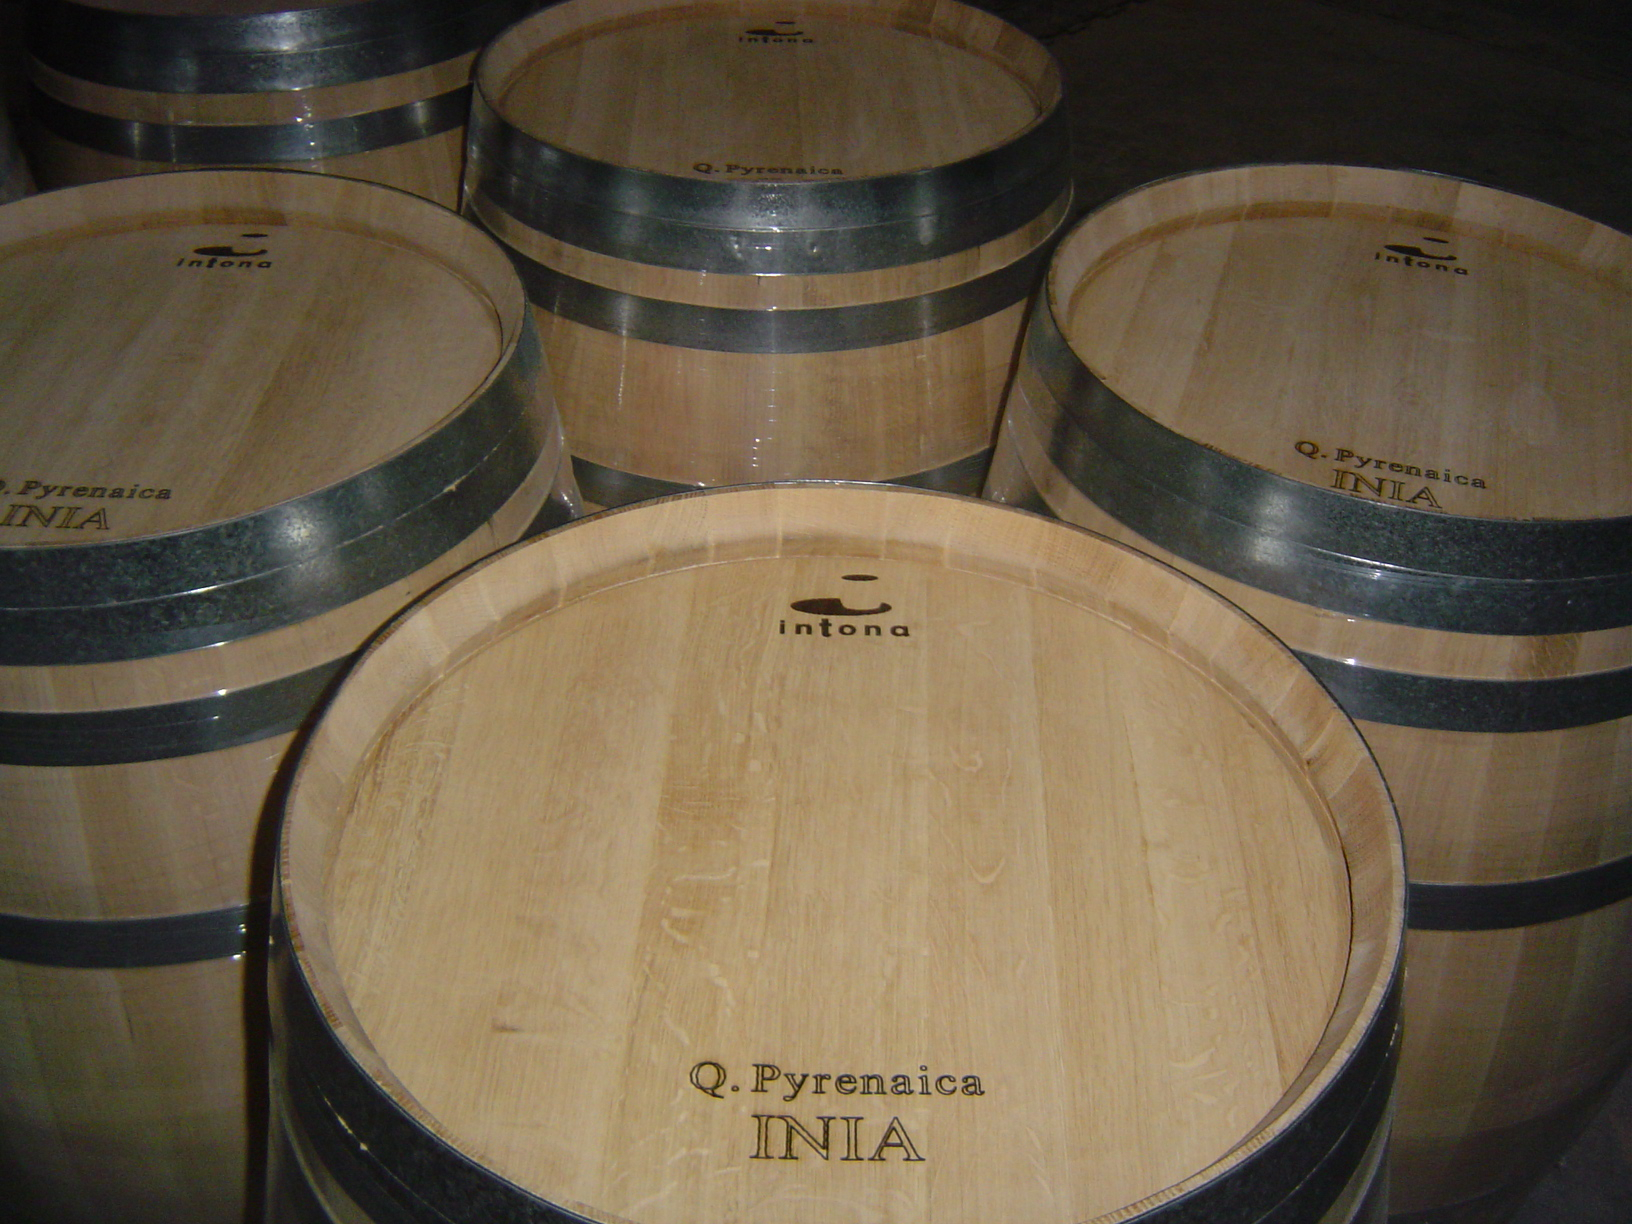
\includegraphics[height=6cm]{img/es/es-barrica.jpg}\caption{Melojo oak barrels for wine aging. Picture from Brigida Fernández de Simón}\label{fig:es:barrica}
\end{figure}

\subsubsection{Edible fungi}\label{sec:es:provision-fungi}
Mycological resources have high ecological, social, recreational and economic importance contributing to increasing the environmental asset value of the forests \autocites{MartinezPenaetal2015RentaAmbiental}. Mushroom picking has increased since 1980s and is becoming a important recreational activity. For European countries, 152 species belonging to 12 genera of wild mushrooms are commonly collected \autocites{Schulpetal2014WildFood}. Data on mushroom production and picking are scarce, scattered and heterogeneous. However, several initiatives have carried out preliminary assessment of mycological resources of forests, such as the RECAMAN initative in Andalusia ("Inncome and Capital of the Andalusian Mountains"; \emph{REnta and the CApital of the Montes de ANdalucía})\autocites{MartinezPenaetal2015RentaAmbiental}. Likewise, the "Plan CUSSTA" (\emph{Plan for the Sustainable Use and Conservation of Mushrooms and Truffles in Andalusia}) is carrying out periodic field sampling to determine the production of mushrooms in different forest formations in Andalusia \autocites{RayaLopezetal2017MuestreosPara}. Preliminary results for three years showed that in \Qp forests, the main marketable species are: \emph{Amanita caesarea} (3.63 \khy), \emph{Boletus aereus} (4.73 \khy), \emph{Cantharellus subpruinosus} (7.8 \khy), \emph{Hydnum rufescens} (0.23 \khy), \emph{Lepista nuda} (0.1 \khy), \emph{Macrolepiota procera} (0.41 \khy) and \emph{Russula cyanoxantha} (0.03 kg \khy). 

\begin{figure}
    \centering
    \includegraphics[height=6cm]{img/es/es-fungi.jpg}\caption{Collection of wild fungi in the surroundings of Robledal de Cáñar}\label{fig:es:fungi}
\end{figure}


\subsubsection{Timber production}\label{sec:es:provision-timber}
The wood of \Qp has not been appreciated as much as that of other oaks, although it has been used to obtain firewood directly or for charcoal production \autocites{MontoyaMeson1979SituacionActual}. For instance, some of the oak populations of Sierra Nevada have been intensely exploited to obtain wood \autocites[\emph{e.g.} Robledal de Cáñar, Alpujarras,][]{ValbuenaCarabanaGil2013GeneticResilience,MorenoLlorcaetal2016HistoricalAnalysis}. In addition, other uses of timber have been documented in this mountain range, such as its use in mining in the northernwestern oak woodlands of Sierra Nevada \autocites{Titos1990}, where the timber of this species was used for mine tunnels and furnaces, and also as firewood to melt the mineral \autocites{Titos1990}. All these heavy exploitation of timber provoked an alteration in the oak forests structure \autocite{PerezLuqueetal2020LanduseLegacies}. Notwithstanding, since the 1970s, anthropogenic pressure on the forests has been reduced, which lead an increase of tree density, and also in the basal area and tree size \autocite{GonzalezDiazetal2020BosquesEspanoles}. This general pattern, observed for the forest of Iberian Peninsula \autocite{Astigarragaetal2020EvidenceNon,GonzalezDiazetal2020BosquesEspanoles}, has been also confirmed for Pyrenean oak forest. Thus, using data from second and third Spanish National Forest Inventory \autocites{VillaescusaDiaz1998SegundoInventario,Villanueva2005TercerInventario}, the temporal variation on tree biomass of the \Qp forests was assessed \autocites{PerezLuqueetal2021CarbonSequestration} (see also chapter \ref{sec:carbon}). The results shown a total increase of 19 172 \mgha between the two national forest inventories, with most of the inventories plot showing an increase pattern (89\%). This increase could be considered an asset for local populations around the oak woodlands, who could use the forest for firewood extraction.

\subsection{Cultural services}\label{sec:es:cultural}
\subsubsection{Recreational values}\label{sec:es:cultural-recreation}
Nature recreation represents a valuable ecosystem service that has a substantial economic value and contributes considerably to income and employment of local communities \autocites{Schagneretal2017MonitoringRecreation}. Monitoring visitors to natural areas have been used to estimate the recreational values provided by several ecosystems \autocites{Andersenetal2014MonitoringVisitors,Schagneretal2017MonitoringRecreation}. We used data from pyroelectric sensors located in several areas of the Sierra Nevada Protected Area to monitor visitors to this mountain range. We selected data located on two singular oak woodlands of Sierra Nevada for which data are available: Dehesa del Camarate, popularly known as \emph{"Bosque Encantado"} (Enchanted Forests), and Vereda de la Estrella. We analyzed the annual profile of the visits (October 2018 to 2019), and compared the visits in the two oak woodlands with total visitors registered for all sensors installed in this mountain region (\emph{n} = 14). Preliminary results showed that those two oak woodlands have a high number of visits, particularly during autumn season, when they represent almost the total number of visits (\figref{fig:es:visitorsprofile}). 

\begin{figure}
    \centering
    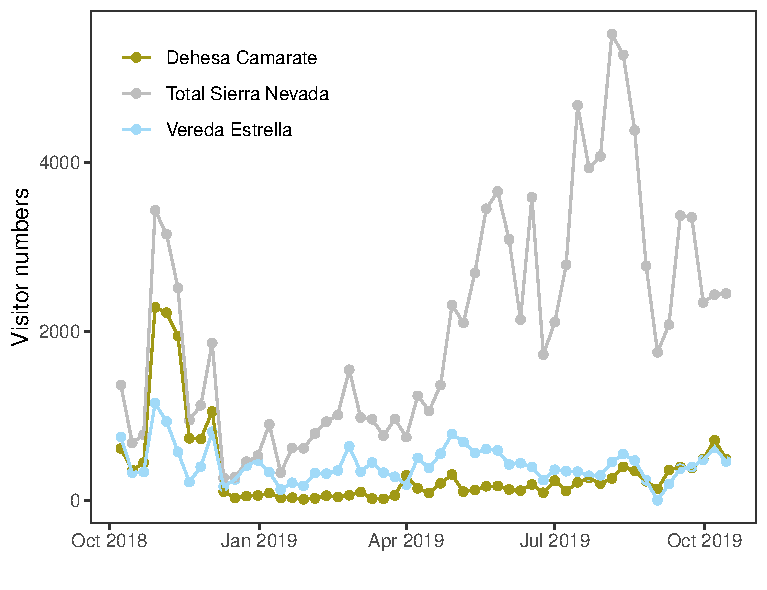
\includegraphics[width=0.9\textwidth]{img/es/es-visitorsprofile.pdf}\caption{Evolution of the visitors numbers in two oak woodlands, \emph{Dehesa del Camarate} (green), and \emph{Vereda de la Estrella} (blue), comparing with the total of Sierra Nevada (gray). Data come from automatic counters (pyroelectric sensors) located at different points in the Sierra Nevada.}\label{fig:es:visitorsprofile}
\end{figure}

\subsubsection{Recreational sports activities}\label{sec:es:cultural-sports}
One way to analyze the physical use of the landscape, and therefore its value as a provider of a cultural ecosystem service, consists of estimating the recreational activities performed in nature \autocites[\emph{e.g.}][]{RocesDiazetal2018AssessingDistribution}. We used the density of routes (hiking, biking, running and other types of outdoor activities) existing in the Wikiloc portal (www.wikiloc.com) (data query in January 2020) for all the municipalities belonging to the Sierra Nevada Natural Protected Area. For each municipality, the total number of routes, and the density (number of routes / surface area of the municipality in ha) were calculated (\tabref{tab:es:wikiloc}). Each of the oak populations of Sierra Nevada were assigned to the municipalities in which they are present. Of the 47998 routes obtained for the Sierra Nevada mountain region, 49.94\% were in the 14 municipalities where oak woodland are present (\figref{fig:es:wikiloc}). The density of routes in these municipalities ranged from 5.24 - 41.8 routes km$^{-2}$ (\tabref{tab:es:wikiloc}) being for most of them much higher than the average density of routes of the Sierra Nevada municipalities (17.88 routes km$^{-2}$). In absolute terms, the municipalities of the Alpujarra have the highest number of routes.

\begin{table}[]
\caption{Wikilock routes density (routes km$^{-2}$), and routes total numbers, for the municipalities of Sierra Nevada where Pyrenean oak woodland are located}
\label{tab:es:wikiloc}
\resizebox{\textwidth}{!}{%
\begin{tabular}{lllllllll}
\toprule
Oak population & CAM & GEN & MON & DIL & DUR & CAN & POQ & TRE \\ \midrule
Tracks density & 18.51 & 13.79 & 35.63 & 14.22 & 24.36 & 32.48 & 52.77 & 29.89 \\
Total tracks & 1170 & 3290 & 3170 & 1140 & 1870 & 555 & 1491 & 1908 \\ \bottomrule
\end{tabular}%
}
\end{table}

\begin{figure}
    \centering
    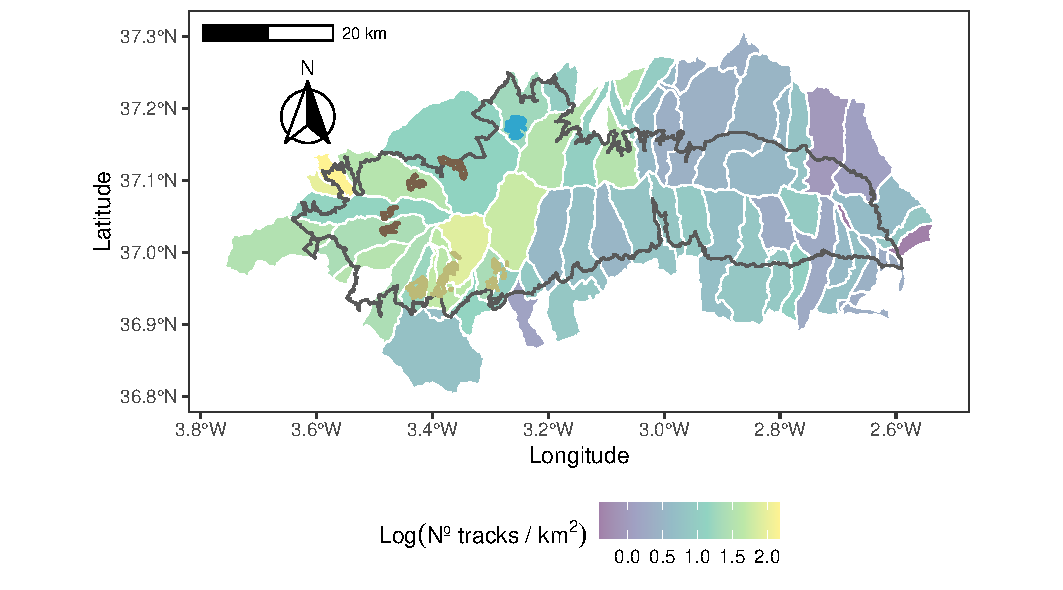
\includegraphics[width=\textwidth]{img/es/es-wikiloc.pdf}\caption{Density of Wikiloc routes for the municipalities of Sierra Nevada (Data from January 2020). Data are shown in Logarithmic scale.}\label{fig:es:wikiloc}
\end{figure}

\subsubsection{Scientific knowledge}\label{sec:es:cultural-scientific} 
To determine the importance of oak woodlands in the supply of the ES scientific knowledge, we used two indicators related to research activities. First, we explore the spatial location of research activities conducted in Sierra Nevada during the period 2009-2013 \autocites{Zamoraetal2017MonitoringGlobal}. For this purpose, a database compiling the research authorization documents for the Sierra Nevada Protected Area, was used to generate a density map with the \emph{hotspots} areas of research activities for Sierra Nevada mountain area. Then we extracted the information for the oak populations. Most of the research authorizations are concentrated in the western side of the Sierra Nevada (\figref{fig:es:scientific}b) particularly in the high summits area. The mean values of research permissions for oak woodlands in the period studied was 3.03 ± 0.06, with Genil and Cáñar oak populations (northwestern and southern oak populations respectively), contain the high concentration of research requests (\figref{fig:es:scientific}b). 
Secondly, we explored a density map of sampling protocols deployed in the Sierra Nevada \autocites{Zamoraetal2017MonitoringGlobal} using data from Sierra Nevada Global Change Observatory \autocites{Zamoraetal2016GlobalChange}. All the social-ecological monitoring protocols within this initiative were geolocated to generate a concentration map of sampling protocols by applying geostatistical hotspot detection techniques (Kernel density estimation) \autocites{Zamoraetal2016GlobalChange} (\figref{fig:es:scientific}a). The results show that the melojo oak woodlands are located in areas of high density of scientific activity (both sampling protocol density and research requested areas) in comparison with the other forest ecosystems of the Sierra Nevada.

\begin{figure}
    \centering
    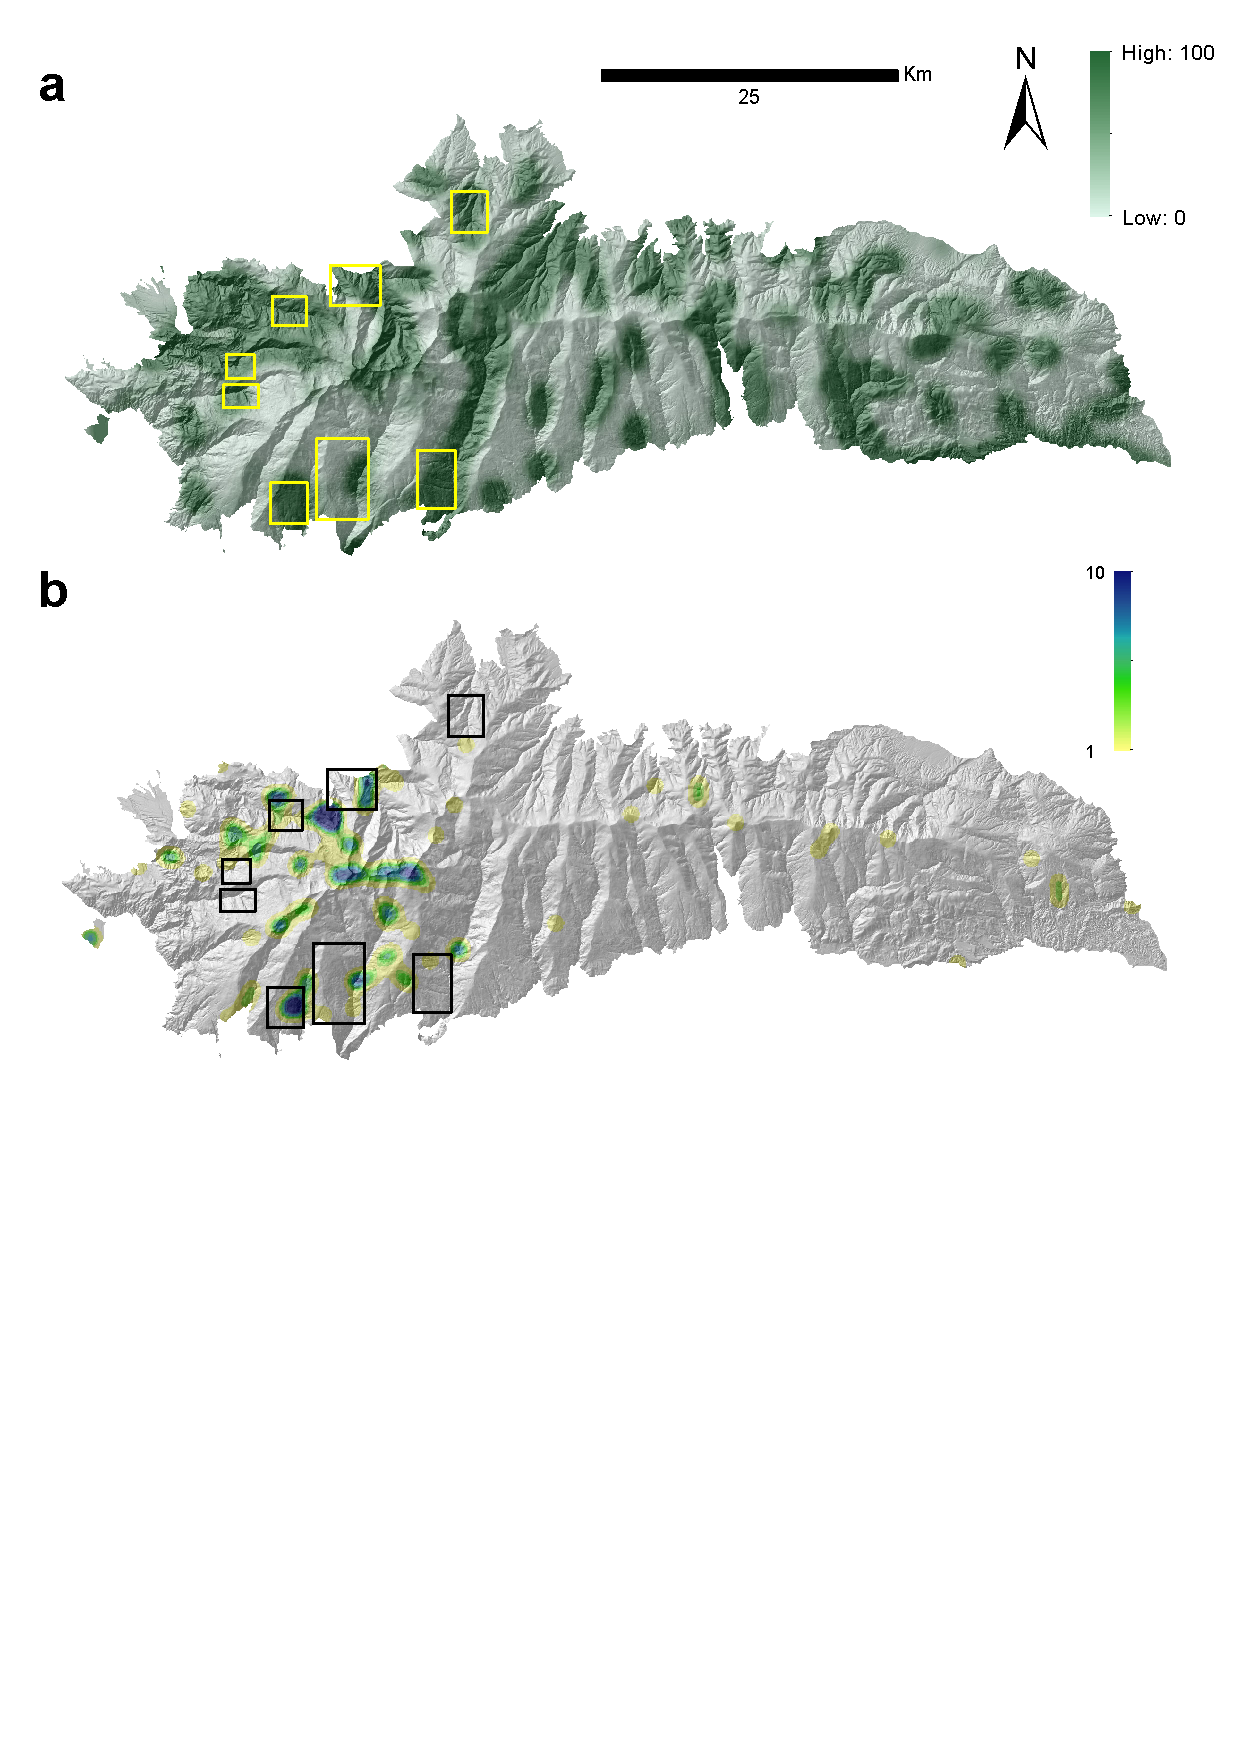
\includegraphics[width=\textwidth]{img/es/es-scientific.pdf}
    \caption{Spatial localization of the research authorizations (Number of research authorizations) performed in Sierra Nevada in the period 2009-2015 (\textbf{a}); and map of density (scaled density) of socioecological monitoring protocols carried out in Sierra Nevada since 2008 (\textbf{b}). For both maps the spatial bounding boxes of each oak population are shown. Drawn from \autocites{Zamoraetal2017MonitoringGlobal,Zamoraetal2016GlobalChange}}\label{fig:es:scientific}
\end{figure}

\subsubsection{Aesthetic values}\label{sec:es:cultural-aesthetic} 
Using data from the Flickr platform (www.flickr.com), \citet{MorenoLlorcaetal2020EvaluatingTourist} assessed some of the cultural services offered in Sierra Nevada. Of the total of 778 photographs analyzed, 18 are geolocated in oak woodlands (\figref{fig:es:flicker}). This value is low with respect to the total number of photographs analyzed, mainly due to the fact that the highest density of photos in the dataset analyzed is located around the ski resort and village areas (mainly the Alpujarras) \autocites{RosCandeiraetal2020SocialMedia}. Likewise, when we explore the various ecosystems in which the photos are located, we observe a higher concentration of photos in the high mountain areas. If we explore forest ecosystems (\emph{i.e.} native pine, holm oak, Pyrenean oak forests, and pine plantations), the photos taken in Pyrenean oak forests represent 32\% of the total.

\subsubsection{Singular trees}\label{sec:es:cultural-trees} 
Singular, large and/or monumental trees perform key ecological functions \autocites[\emph{e.g.} nutrient cycling; support complex assemblages of species,][]{Zapponietal2017RoleMonumental}. They have important impacts on the distribution and abundance of many other entities, from water and nutrients to whole organisms (fungi, other plants and numerous animal species) \autocites{LindenmayerLaurance2017EcologyDistribution}. Furthermore, they are creditors of natural value \emph{perse} \autocites{Asciutoetal2016MonumentalTrees}, and are considered part of a social realm, providing numerous socio-cultural benefits to society \autocites{BlicharskaMikusinski2014IncorporatingSocial,MoyaMoya2013MonumentalTrees}. Singular trees provide humans with aesthetic, symbolic, religious and historical values, as well as concrete tangible benefits, such as leaves, branches or nuts \autocites{BlicharskaMikusinski2014IncorporatingSocial}. They can be considered as single trees by their dasometric (height, diameter at breast height), age, and socio-cultural characteristics (\emph{e.g.} surrounding landscape, local myths, legends and traditions, witnessing historical events), so their conservation could contribute to the protection of both ecological and also social values \autocites{BlicharskaMikusinski2014IncorporatingSocial}. 

\begin{figure}
    \centering
    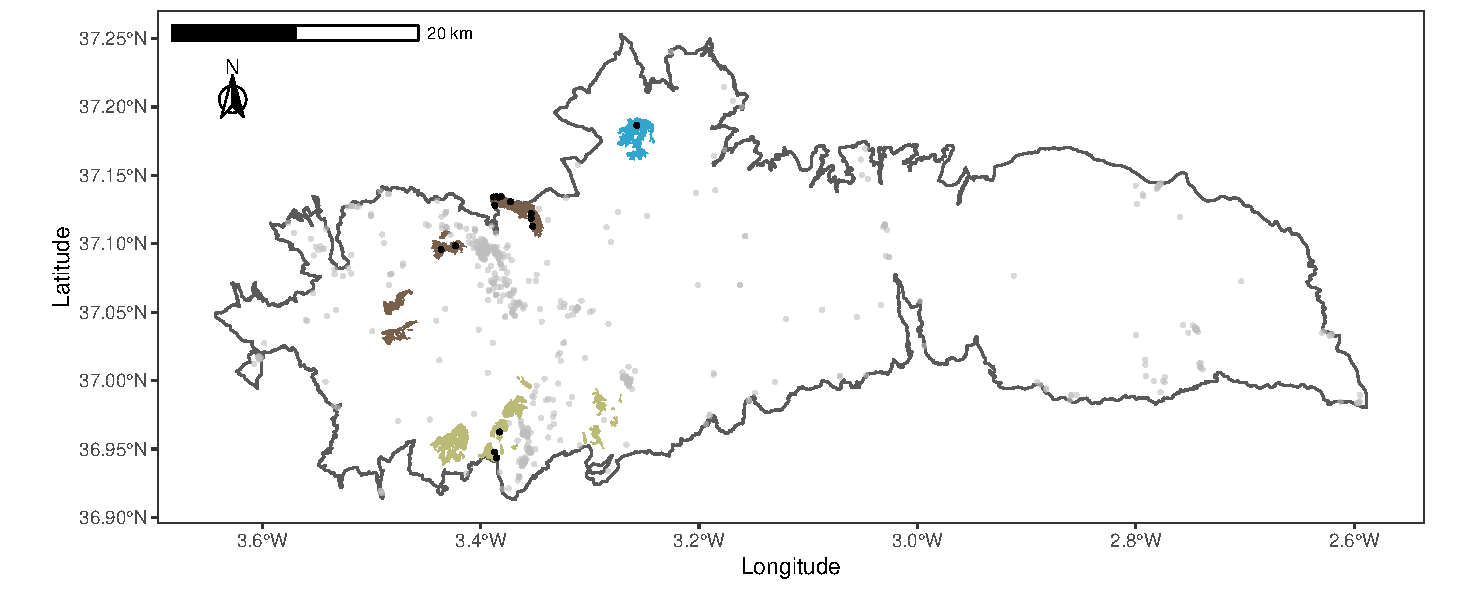
\includegraphics[width=\textwidth]{img/es/es-flicker.pdf}\caption{Location of photos taken in Sierra Nevada uploaded to the Flickr platform (\emph{n} = 778). Black dots indicate photos located in oak woodland. Drawn with data from \citet{RosCandeiraetal2020SocialMedia}. Oak woodland populations are shown. Colors correspond to northern (\emph{blue}), northwestern (\emph{brown}) and southern cluster's of oak woodlands identified for Sierra Nevada \autocite{PerezLuqueetal2021EcologicalDiversity}.  
}\label{fig:es:flicker}
\end{figure}
 
There are several individuals of \Qp in Sierra Nevada considered singular and/or monumental because of their extraordinary dimensions \autocite{IruritaFernandezetal2003ArbolesArboledas}, reaching tree heights of up to 19.5 meters and base perimeter of 6.7 meters. They are located in Busquístar (Alpujarras, southern slopes of Sierra Nevada). There are also other species singular trees located in the surroundings of some meolojo oak populations that add an ecosystem value to these oak populations, since these specimens are visited by hikers. For instance, in the Vereda de la Estrella (Güejar Sierra) there are majestic specimens of chestnut (\emph{Castanea sativa}), with a famous tree known as "El Abuelo" ("The grandpa") standing more than 20 m high and with a perimeter at the base of 10.7 m. Likewise, there are some oak woodlands in Sierra Nevada that shelter specimens and/or singular populations of other species. For instance, the Abedular del Barranco de los Alisos, located in the Dúrcal oak woodland \autocites{MartinezLabargaetal1990AbedularRelictico}. It is a small grove of about 300 individuals of birch (\emph{Betula pendula} subsp. \emph{fontqueri}) with an average height of 12 m. Other examples are the grove of birch trees located at the "Barranco de los Alisos", in the Dúrcal melojo population; or the Aliseda de la Cueva del Santo, where there are more than 100 alders (\emph{Alnus glutinosa}) accompanied by melojo oak and chestnut trees. In Andalusia region, there are also other melojo stands catalogued as singular, such as those located in the Sierra del Aljibe, whose specimens do not stand out for their dimensions but their location is unique and of great interest, representing a southern limit of distribution of the species \autocite{SanchezGarciaetal2003ArbolesArboledas}. 

\subsection{Spatial pattern for Ecosystem Services of Sierra Nevada}\label{sec:es:spatial} 

The quantification of some ES provided by melojo oak populations in Sierra Nevada, allows us to compare the supply of ES among those populations and to describe what ES category predominate for each of the oak population cluster’s in this mountain region. Regarding the regulation services evaluated, we observed that the southern populations have higher values for carbon sequestration potential, mean EVI and soil organic carbon than for the other clusters (\figref{fig:es:oak-compare}), despite the expected greater vulnerability due to their location in the southernmost areas of Sierra Nevada. Those results are in line with previously studies highlighted higher resilience values to disturbance of the southern oak woodlands \autocites{PerezLuqueetal2020LanduseLegacies}. For cultural ecosystem services, the NW populations present high values for sports activities, number of visitors, and density of sampling protocols (scientific value). Finally, for provisioning and support services we observed a variable pattern depending on the ecosystem service evaluated. 

\begin{figure}
    \centering
    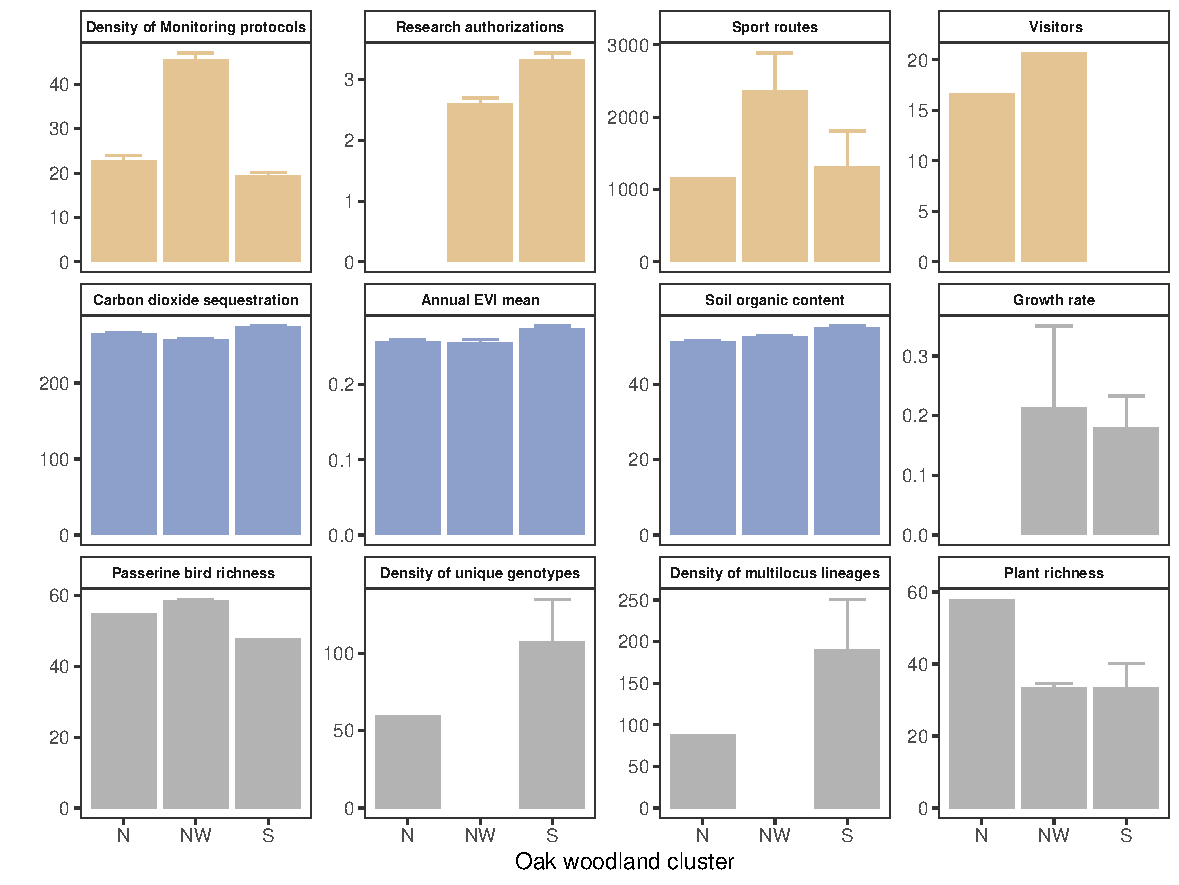
\includegraphics[width=\textwidth]{img/es/es-plotSN.pdf}\caption{Comparison of ecosystem services (cultural: yellow; regulation: blue; supporting: gray) for oak populations cluster identified in Sierra Nevada. See Table \tabref{tab:es:oak-cluster} for a detailed description 
}\label{fig:es:oak-compare}
\end{figure}

\section{Concluding remarks}\label{sec:es:concluding} 
In this work we combined a literature review with expert criterion to identify the ecosystem services provide by \Qp woodlands The literature review revealed the existence of a large number of works related to wine ageing, highlighting the potential of this species for wine production (\tabref{tab:es:wos}). It is striking that no work has been found in our literature review that evaluates cultural services in this woodland forests. However, this pattern changes when the ecosystem services are analyzed in more detail as in our case study. Thus, the combination of expert criteria with data at a more local scale allowed us to highlight the existence of a large number of cultural ecosystem services provided by \Qp woodlands. 
Our review of local data has allowed us to quantify many of the ES provided by melojo oak woodlands, which on the one hand highlights the values of these forest formations, and on the other hand, provides to natural resource managers with more information and tools to help them in the decision-making process. Incorporating information on ecosystem services can help in the planning of forestry actions for those oak woodlands. Our study also adds some interesting insights for the study of ES provided by forests. For instance, we observed a highly temporal pattern of some ES, such as the recreational values. Some melojo woodlands of Sierra Nevada concentrate a large part of the visitors recorded in the Sierra Nevada Natural Area (\figref{fig:es:visitorsprofile}) during a specific time period. This highlighting the needing to consider the temporal pattern of the ES evaluated, and to pay attention to the pressure that these ecosystems may be suffering temporarily due to the high number of visitors they receive. Therefore, from a natural resource management point of view,  it is not only necessary to analyse the ES provided by an ecosystem, but also we would consider the spatio-temporal pattern of the ES supply. In this sense, it would be interesting to carry out detailed studies to provide managers with a comprehensive assessment of the possible impacts of visitors.

\begin{sidewaystable}
\caption{Quantification of several Ecosystem Services (ES) for Sierra Nevada oak population clusters \autocites[see][]{PerezLuqueetal2021EcologicalDiversity}. N: Northern populations, NW: Northwestern populations; S: Southern populations.}\label{tab:es:oak-cluster}
\centering
\scriptsize
\resizebox{\linewidth}{!}{%
\begin{tabular}{>{\hspace{0pt}}m{0.14\linewidth}>{\hspace{0pt}}m{0.402\linewidth}>{\hspace{0pt}}m{0.158\linewidth}>{\centering\hspace{0pt}}m{0.075\linewidth}>{\centering\hspace{0pt}}m{0.085\linewidth}>{\centering\arraybackslash\hspace{0pt}}m{0.077\linewidth}} 
\toprule
\textbf{ES Indicator} & \textbf{Definition} & \textbf{Units} & \textbf{N} & \textbf{NW} & \textbf{S} \\
Plant richness & Mean richness of plant species recorded in forest invetories & Species number & 58 & 33.5 ± 1.04 & 33.5 ± 6.69 \\
Passerine bird richness & Mean richness of passerine birds recorded at bird censuses on oak woodlands & Species number & 55 & 58.5 ± 0.5 & 48 \\
Genetic diversity & Density of genotypes represented by one stem (unique genotypes, GU) per hecatera & Genotypes Uniques ha$^{-1}$ & 60 &  & 107.5 ± 27.5 \\
Genetic diversity & Density of multilocus lineages (MLL) per hectarea & Multiloculs Lineages ha$^{-1}$ & 89 &  & 191 ± 60 \\
Biomass increment & Increment of Biomass amount (Growth rate) between two National Forest Inventories (SNFI2 and SNFI3) & Mg Biomass ha$^{-1}$ year$^{-1}$  &  & 0.214 ± 0.136 & 0.18 ± 0.053 \\
Recreational values & Percentage of visits (visits registered in the oak woodland / total visits registered in Sierra Nevada) & \% & 16.69 & 20.68 &  \\
Sport activities (total routes) & Mean of total routes registered at Wikilock in the Municipalities where oak woodlands are located & Sport activites & 1170 & 2367.5 ± 520.36 & 1318 ± 489.95 \\
Scientific research authorizations & Average values of the Kerneld Density Estimate of the research permissions & Number of autorization research &  & 2.61 ± 0.09 & 3.34 ± 0.1 \\
Scientific sampling density & Average of Normalized Kernel Density Estimation of the Density of Monitoring methodologies & scaled value (0-100) & 22.94 ± 1.07 & 45.56 ± 1.52 & 19.57 ± 0.59 \\
EVI mean & Average of annual EVI mean for all pixels covering oak woodlands populations (period 2000-2018) &  & 0.257 ± 0.003 & 0.256 ± 0.004 & 0.275 ± 0.003 \\
Potential Carbon sequestration & Aveage values of the CO$_2$ potential sequestration & Mg CO$_2$ ha$^{-1}$ & 265.07 ± 1.41 & 256.72 ± 1.05 & 273.91 ± 0.93 \\
SOC & Average values of the mean Soil organic content at a 0-30 cm depth & Mg SOC ha$^{-1}$ & 51.27 ± 0.29 & 52.59 ± 0.34 & 55.11 ± 0.33 \\
\bottomrule
\end{tabular}
}
\end{sidewaystable} 

%\part{Additional Example Part}
%% !TEX root = ../my-thesis.tex
%
\chapter{System}
\label{sec:system}

\cleanchapterquote{Innovation distinguishes between a leader and a follower.}{Steve Jobs}{(CEO Apple Inc.)}

\Blindtext[2][1]

\section{System Section 1}
\label{sec:system:sec1}

\Blindtext[1][2]

\begin{figure}[htb]
	
\includegraphics[width=\textwidth]{img/Clean-Thesis-Figure}
	\caption{Figure example: \textit{(a)} example part one, \textit{(c)} example part two; \textit{(c)} example part three}
	\label{fig:system:example1}
\end{figure}

\Blindtext[1][2]

\section{System Section 2}
\label{sec:system:sec2}

\Blindtext[1][2]

\begin{figure}[htb]
	
\includegraphics[width=\textwidth]{img/Clean-Thesis-Figure}
	\caption{Another Figure example: \textit{(a)} example part one, \textit{(c)} example part two; \textit{(c)} example part three}
	\label{fig:system:example2}
\end{figure}

\Blindtext[2][2]

\section{System Section 3}
\label{sec:system:sec3}

\Blindtext[4][2]

\section{Conclusion}
\label{sec:system:conclusion}

\Blindtext[2][1]
         % INCLUDE: system
%% !TEX root = ../my-thesis.tex
%
\chapter{Concepts: This text is here to test a very long title, to simulate the line break behavior, to show that an extremely long title also works}
\label{sec:concepts}

\cleanchapterquote{Users do not care about what is inside the box, as long as the box does what they need done.}{Jef Raskin}{about Human Computer Interfaces}

\Blindtext[2][1]

\section{Concepts Section 1}
\label{sec:concepts:sec1}

\Blindtext[2][2]

\section{Concepts Section 2 with a very very long title that illustrates how long section titles are handled in the footer}
\label{sec:concepts:sec2}

\Blindtext[3][2]

\section{Concepts Section 3}
\label{sec:concepts:sec3}

\Blindtext[4][2]

\section{Conclusion}
\label{sec:concepts:conclusion}

\Blindtext[2][1]
       % INCLUDE: concepts
% !TEX root = ../my-thesis.tex
%
\chapter{\textcolor{ctcolormain}{Conclusiones}}
\label{sec:conclusion}     % INCLUDE: conclusion

% --------------------------
% Back matter
% --------------------------
%
{%
\setstretch{1.1}
\renewcommand{\bibfont}{\normalfont\small}
\setlength{\biblabelsep}{0pt}
\setlength{\bibitemsep}{0.5\baselineskip plus 0.5\baselineskip}
\printbibliography
%\printbibliography[nottype=online]
%\newrefcontext[labelprefix={@}]
%\printbibliography[heading=subbibliography,title={Webpages},type=online]
}%
\cleardoublepage

%\listoffigures
%\cleardoublepage

%\listoftables
%\cleardoublepage

%\lstlistoflistings
%\cleardoublepage

\part{Apéndices}
\appendix\cleardoublepage
% !TEX root = ../my-thesis.tex
%
\chapter{Material Suplementario del  \autoref{sec:multivar}}\label{sec:appendix:multivar}

{%
\scriptsize
\begin{longtable}{llllllllll}
\caption{Species present in each population.}\label{tab:multivar-s1}\\ 
\toprule
 \textbf{Scientific name}  & \textbf{CAM}  & \textbf{GEN}  & \textbf{MON}  & \textbf{DIL}  & \textbf{DUR}  & \textbf{CAN}  & \textbf{POQ}  & \textbf{TRE}  \endfirsthead 
\hline
\textit{Acer opalus }subsp\textit{. granatense}  & 1 &  & 1 & 1 &  &  &  &  \\
\textit{Adenocarpus decorticans}  & 1 & 1 & 1 & 1 & 1 &  & 1 & 1 \\
\textit{Agrostis canina}  & 1 &  &  &  &  &  &  &  \\
\textit{Andryala integrifolia}  &  &  &  &  &  &  &  & 1 \\
\textit{Arenaria armerina }subsp\textit{. armerina}  & 1 &  &  &  &  &  &  &  \\
\textit{Armeria villosa }subsp\textit{. bernisii}  & 1 &  & 1 &  & 1 &  &  &  \\
\textit{Arrhenatherum elatius }subsp\textit{. bulbosum}  &  &  &  & 1 &  & 1 &  &  \\
\textit{Artemisia absinthium}  &  &  &  &  & 1 &  &  &  \\
\textit{Artemisia barrelieri}  &  &  &  &  & 1 &  &  &  \\
\textit{Artemisia campestris }subsp\textit{. glutinosa}  & 1 & 1 & 1 & 1 & 1 & 1 &  & 1 \\
\textit{Avenula bromoides }subsp\textit{. pauneroi}  &  & 1 & 1 & 1 & 1 &  &  &  \\
\textit{Berberis hispanica}  & 1 &  & 1 & 1 &  &  &  & 1 \\
\textit{Brachypodium retusum}  &  &  &  & 1 &  &  &  & 1 \\
\textit{Carlina corymbosa}  & 1 &  &  &  & 1 &  & 1 & 1 \\
\textit{Carthamus lanatus}  &  & 1 &  &  & 1 & 1 &  & 1 \\
\textit{Celtis australis}  &  &  & 1 &  &  &  &  &  \\
\textit{Centaurea monticola}  &  &  &  &  &  &  & 1 &  \\
\textit{Centaurea ornata}  & 1 &  &  &  &  &  &  &  \\
\textit{Centaurea pulvinata}  &  &  & 1 &  &  &  &  &  \\
\textit{Cerastium gibraltaricum}  & 1 &  & 1 &  & 1 &  &  & 1 \\
\textit{Chondrilla juncea}  & 1 &  &  &  &  &  &  &  \\
\textit{Cirsium odontolepis}  &  &  &  &  & 1 &  &  &  \\
\textit{Cirsium pyrenaicum}  &  &  &  &  &  &  &  & 1 \\
\textit{Clematis vitalba}  &  &  &  & 1 &  &  &  &  \\
\textit{Clinopodium vulgare }subsp\textit{. arundanum}  & 1 &  & 1 &  &  &  &  &  \\
\textit{Corynephorus canescens}  &  &  & 1 & 1 &  &  &  &  \\
\textit{Cotoneaster granatensis}  & 1 &  &  & 1 & 1 &  &  &  \\
\textit{Crataegus granatensis}  & 1 &  &  &  &  &  &  &  \\
\textit{Crataegus monogyna }subsp\textit{. brevispina}  & 1 & 1 & 1 & 1 & 1 &  &  & 1 \\
\textit{Crocus nevadensis}  & 1 &  &  &  &  &  &  &  \\
\textit{Cytisus galianoi}  & 1 &  &  &  &  &  &  &  \\
\textit{Cytisus scoparius }subsp\textit{. reverchonii}  & 1 &  & 1 & 1 & 1 &  &  &  \\
\textit{Dactylis glomerata}  & 1 & 1 &  &  &  &  &  &  \\
\textit{Dactylis glomerata }subsp\textit{. hispanica}  &  &  & 1 & 1 & 1 & 1 &  &  \\
\textit{Daphne gnidium}  &  &  &  &  &  &  &  & 1 \\
\textit{Dianthus pungens }subsp\textit{. brachyanthus}  &  &  & 1 & 1 & 1 &  &  &  \\
\textit{Digitalis purpurea}  &  & 1 &  &  &  &  &  &  \\
\textit{Echinospartum boissieri}  &  &  & 1 &  &  &  &  &  \\
\textit{Elymus hispanicus}  & 1 &  &  &  &  &  &  &  \\
\textit{Erinacea anthyllis}  &  &  &  &  &  &  &  & 1 \\
\textit{Eryngium campestre}  & 1 & 1 & 1 &  &  &  & 1 & 1 \\
\textit{Euphorbia characias}  &  &  &  &  & 1 &  & 1 & 1 \\
\textit{Euphorbia nevadensis}  &  &  &  &  & 1 &  &  &  \\
\textit{Festuca elegans}  & 1 &  & 1 &  &  &  &  & 1 \\
\textit{Festuca hystrix}  &  &  & 1 & 1 &  &  &  &  \\
\textit{Festuca indigesta}  & 1 &  &  & 1 & 1 & 1 &  & 1 \\
\textit{Festuca scariosa}  & 1 & 1 &  &  &  &  &  &  \\
\textit{Fraxinus angustifolia}  &  & 1 &  &  &  &  &  &  \\
\textit{Genista cinerea }subsp\textit{. speciosa}  &  &  & 1 &  &  &  &  &  \\
\textit{Genista versicolor}  & 1 &  &  & 1 & 1 & 1 &  & 1 \\
\textit{Halimium atriplicifolium}  &  &  &  & 1 &  &  &  & 1 \\
\textit{Helianthemum hirtum}  & 1 &  & 1 &  & 1 &  &  &  \\
\textit{Helichrysum italicum }subsp\textit{. serotinum}  &  &  &  &  &  & 1 & 1 & 1 \\
\textit{Helleborus foetidus}  & 1 & 1 & 1 & 1 &  &  &  & 1 \\
\textit{Hieracium pilosella }subsp\textit{. tricholepium}  & 1 &  &  &  &  & 1 &  &  \\
\textit{Hormatophylla spinosa}  & 1 &  &  &  & 1 &  &  &  \\
\textit{Hypericum perforatum}  &  &  & 1 &  & 1 &  & 1 & 1 \\
\textit{Juncus effusus}  &  &  &  &  &  &  & 1 &  \\
\textit{Juniperus communis}  & 1 &  &  &  &  &  &  &  \\
\textit{Juniperus sabina}  & 1 &  &  &  &  &  &  &  \\
\textit{Koeleria vallesiana}  & 1 &  &  & 1 & 1 & 1 & 1 &  \\
\textit{Lathyrus pratensis}  &  &  &  &  & 1 &  &  &  \\
\textit{Lonicera arborea}  & 1 & 1 &  &  & 1 &  &  &  \\
\textit{Marrubium supinum}  & 1 &  &  &  &  &  & 1 & 1 \\
\textit{Ononis aragonensis}  &  &  & 1 & 1 &  &  &  &  \\
\textit{Ononis spinosa}  &  & 1 &  & 1 &  &  & 1 &  \\
\textit{Phlomis crinita}  &  &  &  &  &  &  &  & 1 \\
\textit{Pistacia terebinthus}  &  & 1 &  &  &  &  &  &  \\
\textit{Plantago lanceolata}  &  &  &  &  &  &  &  & 1 \\
\textit{Plantago radicata }subsp\textit{. granatensis}  & 1 &  &  &  &  &  &  &  \\
\textit{Populus nigra}  &  &  &  &  & 1 &  &  &  \\
\textit{Potentilla reuteri}  & 1 &  &  &  & 1 &  &  &  \\
\textit{Prunus avium}  & 1 & 1 &  &  &  &  &  &  \\
\textit{Prunus dulcis}  &  & 1 &  &  &  &  &  &  \\
\textit{Prunus mahaleb}  & 1 &  &  &  &  &  &  &  \\
\textit{Prunus ramburii}  & 1 &  &  &  &  &  &  & 1 \\
\textit{Ptilostemon hispanicus}  &  &  &  &  &  & 1 &  & 1 \\
\textit{Quercus coccifera}  &  & 1 &  &  &  &  &  &  \\
\textit{Quercus faginea}  &  & 1 &  &  &  &  &  &  \\
\textit{Quercus ilex }subsp\textit{. ballota}  & 1 &  & 1 &  & 1 & 1 & 1 & 1 \\
\textit{Quercus pyrenaica}  & 1 & 1 & 1 & 1 & 1 & 1 & 1 & 1 \\
\textit{Retama sphaerocarpa}  &  &  & 1 &  &  &  &  &  \\
\textit{Ridolfia segetum}  &  & 1 &  &  &  &  &  & 1 \\
\textit{Rosa canina}  & 1 & 1 & 1 & 1 & 1 &  & 1 & 1 \\
\textit{Rosa corymbifera}  & 1 &  &  &  &  &  &  &  \\
\textit{Rosa micrantha}  &  &  &  &  &  &  &  & 1 \\
\textit{Rosa pouzinii}  & 1 &  &  &  &  &  &  &  \\
\textit{Rosa sicula}  & 1 &  &  &  &  &  &  &  \\
\textit{Rubus ulmifolius}  & 1 & 1 &  & 1 & 1 &  &  & 1 \\
\textit{Rumex induratus}  &  &  &  & 1 &  &  &  &  \\
\textit{Salix caprea}  &  &  & 1 &  &  &  &  &  \\
\textit{Sanguisorba minor}  & 1 &  &  & 1 &  &  & 1 &  \\
\textit{Santolina rosmarinifolia }subsp\textit{. canescens}  &  &  &  & 1 &  &  &  &  \\
\textit{Santolina rosmarinifolia }subsp\textit{. rosmarinifolia}  & 1 & 1 &  &  &  &  &  &  \\
\textit{Scabiosa turolensis}  & 1 &  &  &  &  &  &  &  \\
\textit{Sedum forsteranum}  & 1 &  &  &  &  &  &  &  \\
\textit{Sedum sediforme}  & 1 &  &  &  &  &  &  & 1 \\
\textit{Silene mellifera}  &  &  & 1 & 1 &  &  & 1 &  \\
\textit{Smilax aspera}  &  & 1 &  &  &  &  &  &  \\
\textit{Solidago virgaurea}  &  &  & 1 &  &  &  &  &  \\
\textit{Sorbus aria}  & 1 &  & 1 &  &  &  &  &  \\
\textit{Teucrium capitatum}  &  &  & 1 &  &  &  &  &  \\
\textit{Teucrium similatum}  & 1 &  &  &  &  &  &  &  \\
\textit{Thymus mastichina}  & 1 &  &  & 1 &  & 1 &  & 1 \\
\textit{Thymus serpylloides }subsp\textit{. serpylloides}  &  &  &  &  &  & 1 &  & 1 \\
\textit{Thymus zygis}  &  &  &  &  &  &  & 1 & 1 \\
\textit{Vicia sp.}  &  & 1 & 1 &  & 1 &  &  &  \\
\textit{Vinca difformis}  &  &  &  & 1 &  &  &  &  \\ 
\hline
\textbf{Total}  & 54 & 25 & 34 & 31 & 32 & 14 & 17 & 36 \\
\bottomrule
\end{longtable}

}%

\newpage

\chapter{Material Suplementario del Capítulo \ref{sec:carbon}}\label{sec:appendix:carbon}
\newpage

\begin{sidewaystable} 
\caption{Predictor variables selected for each model obtained to estimate each biomass fraction from LIDAR data.}
\label{tab:carbon:lidarmodels}
\begin{adjustbox}{width=\linewidth}
\begin{threeparttable}
\begin{tabular}{@{}llccc@{}}
\footnotesize
\textbf{Biomass fraction} & \textbf{Predictors} & \textbf{RMSE} & \textbf{RMSE (\%)} & \textbf{R$^2$} \\ \toprule
\multirow{4}{*}{\textbf{\ws}} & Rumple index & \multirow{4}{*}{64.1} & \multirow{4}{*}{54.5} & \multirow{4}{*}{0.4489} \\
 & Elevation (m) &  &  &  \\
 & 99th percentile of canopy height (m) &  &  &  \\
 & Maximum canopy height (m) &  &  &  \\ \midrule
\multirow{6}{*}{\textbf{\wro}} & Rumple index & \multirow{6}{*}{25} & \multirow{6}{*}{49.4} & \multirow{6}{*}{0.3364} \\
 & Cover estimate (\%) (All\_cover\_above\_mean) &  &  &  \\
 & Elevation (m) &  &  &  \\
 & 99th percentile of canopy height (m) &  &  &  \\
 & Proportion of returns with   height between 2-5m compared to all returns (\%) &  &  &  \\
 & Maximum canopy height (m) &  &  &  \\ \midrule
\multirow{7}{*}{\textbf{\wb}} & Rumple index & \multirow{7}{*}{3.9} & \multirow{7}{*}{44.2} & \multirow{7}{*}{0.1681} \\
 & Elevation (m) &  &  &  \\
 & Canopy cover (\%) (FIRST\_RETURNS\_1st\_cover\_above\_mean) &  &  &  \\
 & Canopy cover (\%) (FIRST\_RETURNS\_all\_1st\_cover\_above\_mean) &  &  &  \\
 & CV canopy height (m) (FIRST\_RETURNS\_elev\_CV\_0p5plus) &  &  &  \\
 & 99th percentile of canopy height (m) &  &  &  \\
 & Proportion of returns with   height between 2-5m compared to all returns (\%) &  &  &  \\ \midrule
\multirow{4}{*}{\textbf{\wbs}} & Rumple index & \multirow{4}{*}{9.2} & \multirow{4}{*}{52} & \multirow{4}{*}{0.4761} \\
 & Elevation (m) &  &  &  \\
 & 99th percentile of canopy height (m) &  &  &  \\
 & Maximum canopy height (m) &  &  &  \\ \midrule
\multirow{4}{*}{\textbf{\wt}} & Rumple index & \multirow{4}{*}{94} & \multirow{4}{*}{48} & \multirow{4}{*}{0.4761} \\
 & Elevation (m) &  &  &  \\
 & 99th percentile of canopy height (m) &  &  &  \\
 & Maximum canopy height (m) &  &  & 
\end{tabular}
\end{threeparttable}
\end{adjustbox}
\end{sidewaystable}
\normalsize 


\begin{sidewaystable} 
\caption{Biomass (\mgha) and Potential carbon sequestration (\mgha) values for Pyrenean oak populations in Sierra Nevada. Different letters indicate statistically significant differences between sites (Kruskal–Wallis test followed by Dunns test, p \textless 0.05). }
\label{tab:carbon:biomass-pop}
\begin{adjustbox}{width=\linewidth}
\begin{threeparttable}
\begin{tabular}{l|c|c|c|c|c|c|c|c} \toprule
 & \multicolumn{8}{c}{\textbf{Pyrenean oak population}} \\ \midrule
 & \textbf{CAM} & \textbf{GEN} & \textbf{MON} & \textbf{DIL} & \textbf{DUR} & \textbf{CAN} & \textbf{POQ} & \textbf{TRE} \\ \toprule
\textbf{\ws} & 84.29 ± 0.50 a & 82.50 ± 0.46 a & 109.32 ± 0.83 d & 68.61 ± 0.97 c & 63.71 ± 0.88 c & 93.51 ± 0.51 b & 86.85 ± 0.51 e & 85.06 ± 0.75 ae \\
\textbf{\wbs} & 8.71 ± 0.04 a & 8.15 ± 0.03 e & 9.90 ± 0.06 f & 7.41 ± 0.07 c & 7.11 ± 0.07 d & 8.36 ± 0.03 b & 8.44 ± 0.04 g & 8.25 ± 0.05 b \\
\textbf{\wb} & 13.16 ± 0.08 a & 13.01 ± 0.08 a & 17.17 ± 0.14 d & 10.88 ± 0.16 c & 9.85 ± 0.14 c & 14.91 ± 0.09 b & 13.81 ± 0.09 e & 13.47 ± 0.13 ae \\
\textbf{\wro} & 49.32 ± 0.21 a & 43.80 ± 0.18 e & 60.33 ± 0.35 f & 41.70 ± 0.44 c & 39.30 ± 0.38 d & 48.47 ± 0.19 ab & 47.79 ± 0.21 b & 46.07 ± 0.29 g \\
\textbf{\wt} & 152.06 ± 0.81 a & 142.12 ± 0.74 d & 193.77 ± 1.37 e & 124.91 ± 1.59 c & 117.67 ± 1.45 c & 162.95 ± 0.83 b & 154.21 ± 0.84 f & 151.19 ± 1.22 a \\
\textbf{\cro} & 85.98 ± 0.37 a & 76.36 ± 0.32 e & 105.17 ± 0.61 f & 72.69 ± 0.76 c & 68.51 ± 0.66 d & 84.50 ± 0.33 ab & 83.32 ± 0.37 b & 80.31 ± 0.51 g \\
\textbf{\cs} & 146.93 ± 0.86 a & 143.82 ± 0.80 a & 190.57 ± 1.45 d & 119.61 ± 1.69 c & 111.06 ± 1.53 c & 163.01 ± 0.89 b & 151.40 ± 0.89 e & 148.28 ± 1.31 ae \\
\textbf{\cb} & 22.95 ± 0.15 a & 22.68 ± 0.13 a & 29.93 ± 0.24 d & 18.97 ± 0.28 c & 17.17 ± 0.25 c & 25.99 ± 0.15 b & 24.08 ± 0.15 e & 23.48 ± 0.22 ae \\
\textbf{\cbs} & 15.19 ± 0.06 a & 14.22 ± 0.05 e & 17.26 ± 0.11 f & 12.92 ± 0.13 c & 12.40 ± 0.12 d & 14.57 ± 0.06 b & 14.71 ± 0.06 g & 14.38 ± 0.09 b \\
\textbf{\ct}& 265.07 ± 1.41 a & 247.74 ± 1.29 d & 337.79 ± 2.38 e & 217.76 ± 2.78 c & 205.12 ± 2.53 c & 284.07 ± 1.44 b & 268.83 ± 1.46 f & 263.56 ± 2.13 a \\ \bottomrule
\end{tabular}
\end{threeparttable}
\end{adjustbox}
\end{sidewaystable}

\begin{sidewaystable} 
\caption{Model selection for total (\wt), stem (\ws), and root (\wro) biomass (\mgha). Models selected in terms of BIC ($\Delta$ BIC \textless 2 units) are indicated in bold.}
\label{tab:carbon:model-selection}
\begin{adjustbox}{width=\linewidth}
\begin{threeparttable}
\begin{tabular}{@{}l|lrrrrr@{}}
\textbf{Response} & \textbf{covariates} & \textbf{df} & \textbf{logLik} & \textbf{BIC} & \textbf{$\Delta$ BIC} & \textbf{weight} \\ \midrule
\multirow{5}{*}{\textbf{\wt}} & \textbf{Ln Tree density + elevation + Structural diversity index + Structural diversity index:Ln Tree density} & \textbf{6} & \textbf{-592.02} & \textbf{1212.0} & \textbf{0.00} & \textbf{0.595} \\
 & elevation & 3 & -600.47 & 1214.9 & 2.91 & 0.139 \\
 & Ln Tree density + elevation + Structural diversity index & 5 & -596.15 & 1215.6 & 3.60 & 0.098 \\
 & Ln Tree density + elevation + Structural diversity index + Structural diversity index:Ln Tree density + Structural diversity index:elevation & 7 & -591.57 & 1215.8 & 3.76 & 0.091 \\
 & elevation +  Structural diversity index & 4 & -598.72 & 1216.1 & 4.06 & 0.078 \\ \midrule
\multirow{5}{*}{\textbf{\ws}} & \textbf{Ln Tree density + elevation + Structural diversity index + Structural diversity index:Ln Tree density} & \textbf{6} & \textbf{-545.46} & \textbf{1118.9} & \textbf{0.00} & \textbf{0.672} \\
 & Ln Tree density + elevation + Structural diversity index + Structural diversity index:Ln Tree density + Structural diversity index:elevation & 7 & -544.96 & 1122.6 & 3.67 & 0.107 \\
 & Ln Tree density + elevation + twi + Structural diversity index + Structural diversity index:Ln Tree density & 7 & -545.12 & 1122.9 & 3.99 & 0.091 \\
 & Ln Tree density + elevation + Structural diversity index + elevation:Ln Tree density + Structural diversity index:Ln Tree density & 7 & -545.46 & 1123.6 & 4.66 & 0.065 \\
 & elevation +  Structural diversity index & 4 & -552.47 & 1123.6 & 4.70 & 0.064 \\ \midrule
\multirow{5}{*}{\textbf{\wro}} & elevation & 3 & -443.77 & 901.5 & 0.00 & 0.431 \\
 & Ln Tree density + elevation & 4 & -442.15 & 903.0 & 1.43 & 0.211 \\
 & \textbf{Ln Tree  density + elevation + Structural diversity index + Structural diversity index:Ln Tree density} & \textbf{6} & \textbf{-437.67} & \textbf{903.3} & \textbf{1.78} & \textbf{0.177} \\
 & elevation +  twi + twi:elevation & 5 & -440.48 & 904.3 & 2.75 & 0.109 \\
 & elevation +  twi & 4 & -443.23 & 905.1 & 3.58 & 0.072
\end{tabular}
\end{threeparttable}
\end{adjustbox}
\end{sidewaystable}




\chapter{Material Suplementario del  \autoref{sec:dendro}}\label{sec:appendix:dendro}

\begin{table}[ht]
\caption{Robust two-way ANOVAs of the resilience metrics of greenness (EVI) and tree growth (BAI) for the two drought events (in 2005 and 2012) and site.}
\label{tab:dendro:robustanova}
\begingroup\fontsize{8}{10}\selectfont
\begin{tabular}{@{}llllrllrllr@{}}
\toprule
 &  &  & \textbf{Resistance} &  &  & \textbf{Recovery} &  &  & \textbf{Resilience} &  \\ \midrule
 & \textbf{Factor} &  & \textbf{F} & \textit{p} &  & \textbf{F} & \textit{p} &  & \textbf{F} & \textit{p} \\ \cmidrule(lr){4-5} \cmidrule(lr){7-8} \cmidrule(l){10-11} 
\multirow{3}{*}{EVI} & Drought event &  & 799.9 & \textless 0.001 &  & 312.0 & \textless 0.001 &  & 207.2 & \textless 0.001 \\
 & Site &  & 153.2 & \textless 0.001 &  & 105.4 & \textless 0.001 &  & 29.8 & \textless 0.001 \\
 & Drought event $\times$ Site &  & 234.7 & \textless 0.001 &  & 364.3 & \textless 0.001 &  & 6.1 & 0.014 \\ \midrule
\multirow{3}{*}{BAI} & Drought event &  & 6.0 & 0.019 &  & 29.5 & \textless 0.001 &  & 44.3 & \textless 0.001 \\
 & Site &  & 59.3 & \textless 0.001 &  & 53.1 & \textless 0.001 &  & 1.3 & 0.534 \\
 & Drought event $\times$ Site &  & 32.2 & \textless 0.001 &  & 4.4 & 0.134 &  & 30.0 & \textless 0.001 \\ \bottomrule
\end{tabular}
\endgroup{}
\end{table}

\begin{table}[h]
\caption{Drought events for the 1901-2016 period for Sierra Nevada ranked according to drought severity calculated from the SPEI index (12 months scale).}
\label{tab:dendro:droughts}
\centering
\begingroup\fontsize{9}{10}\selectfont
\begin{tabular}{@{}cccccc@{}}
\toprule
\textbf{Duration (months)} & \textbf{Intensity} & \textbf{Severity} & \textbf{Lowest SPEI} & \textbf{Months} & \textbf{Year} \\ \midrule
11 & -1.957 & 21.524 & -2.585 & Jan - Nov & 1995 \\
11 & -1.581 & 17.391 & -2.024 & Nov - Sep & 1913-1914 \\
9 & -1.823 & 16.409 & -2.42 & May - Jan & 1945-1946 \\
9 & -1.764 & 15.88 & -2.056 & Dec - Aug & 1998-1999 \\
8 & -1.482 & 11.859 & -1.654 & Feb - Sep & 1983 \\
6 & -1.728 & 10.367 & -1.906 & Mar - Aug & 2012 \\
5 & -1.905 & 9.527 & -2.3 & Jan - May & 1925 \\
5 & -1.522 & 7.611 & -1.571 & May - Sep & 2005 \\
5 & -1.493 & 7.463 & -1.537 & May - Sep & 1985 \\
5 & -1.385 & 6.926 & -1.444 & Apr - Aug & 1991 \\
4 & -1.714 & 6.855 & -1.833 & May - Aug & 1931 \\
4 & -1.363 & 5.453 & -1.441 & May - Aug & 1927 \\ \bottomrule
\end{tabular}
\endgroup{}
\end{table}


\begin{sidewaystable} 
\caption{Robust measures of central tendency of resilience indices for greenness (EVI) and tree growth (BAI), grouped by drought events, site, and interaction. Measures of central tendency are M-estimators based on Huber’s Psi. In parentheses are the 95\% confidence intervals using 3000 bootstraps. Total corresponds to the average of 2005 and 2012}
\label{tab:dendro:huber}
\begin{adjustbox}{width=\linewidth}
\begin{threeparttable}
\begin{tabular}{@{}ll|ccc|ccc|cccl@{}}
 &  & \multicolumn{1}{l}{} & \textbf{2005} & \multicolumn{1}{l|}{} & \multicolumn{1}{l}{} & \textbf{2012} & \multicolumn{1}{l|}{} & \multicolumn{1}{l}{} & \textbf{Total} & \multicolumn{1}{l}{} &  \\ \cmidrule(r){1-11}
\textbf{Variable} & \textbf{Sites} & \textbf{Resistance} & \textbf{Recovery} & \textbf{Resilience} & \textbf{Resistance} & \textbf{Recovery} & \textbf{Resilience} & \textbf{Resistance} & \textbf{Recovery} & \textbf{Resilience} &  \\ \cmidrule(r){1-11}
\textbf{EVI} & Northern slope & 0.819 & 1.169 & 0.955 & 0.947 & 1.042 & 0.986 & 0.884 & 1.102 & 0.97 &  \\
 &  & (0.814 - 0.824) & (1.161 - 1.177) & (0.951 - 0.960) & (0.942 - 0.952) & (1.036 - 1.047) & (0.980 - 0.990) & (0.878 - 0.889) & (1.096 - 1.108) & (0.967 - 0.974) &  \\ \cmidrule(lr){2-11}
 & Southern slope & 0.902 & 1.066 & 0.962 & 0.939 & 1.071 & 1.004 & 0.921 & 1.069 & 0.983 &  \\
 &  & (0.896 - 0.907) & (1.058 - 1.074) & (0.957 - 0.966) & (0.934 - 0.944) & (1.067 - 1.075) & (1.000 - 1.008) & (0.917 - 0.925) & (1.065 - 1.073) & (0.980 - 0.986) &  \\ \cmidrule(lr){2-11}
 & All & 0.858 & 1.12 & 0.958 & 0.943 & 1.057 & 0.995 &  &  &  &  \\
 &  & (0.854 - 0.863) & (1.113 - 1.126) & (0.955 - 0.962) & (0.940 - 0.947) & (1.054 - 1.060) & (0.991 - 0.998) &  &  &  &  \\ \cmidrule(r){1-11}
\textbf{BAI} & CA-High & 0.892 & 0.887 & 0.79 & 0.753 & 1.107 & 0.813 & 0.816 & 0.996 & 0.798 &  \\
 &  & ( 0.809 - 0.975) & ( 0.800 - 0.973) & ( 0.691 - 0.888) & ( 0.686 - 0.820) & ( 1.026 - 1.188) & ( 0.741 - 0.885) & ( 0.755 - 0.876) & ( 0.917 - 1.075) & ( 0.744 - 0.851) &  \\ \cmidrule(lr){2-11}
 & CA-Low & 0.901 & 0.832 & 0.73 & 0.926 & 0.952 & 0.876 & 0.921 & 0.897 & 0.817 &  \\
 &  & ( 0.813 - 0.989) & ( 0.733 - 0.932) & ( 0.612 - 0.849) & ( 0.900 - 0.953) & ( 0.889 - 1.015) & ( 0.839 - 0.913) & ( 0.883 - 0.958) & ( 0.843 - 0.951) & ( 0.755 - 0.879) &  \\ \cmidrule(lr){2-11}
 & SJ & 0.445 & 1.112 & 0.489 & 0.769 & 1.446 & 1.031 & 0.612 & 1.282 & 0.769 &  \\
 &  & ( 0.375 - 0.516) & ( 1.000 - 1.224) & ( 0.421 - 0.556) & ( 0.684 - 0.853) & ( 1.322 - 1.569) & ( 0.930 - 1.132) & ( 0.539 - 0.685) & ( 1.179 - 1.386) & ( 0.652 - 0.886) &  \\ \cmidrule(lr){2-11}
 & All & 0.721 & 0.946 & 0.653 & 0.819 & 1.161 & 0.911 &  &  &  &  \\
 &  & ( 0.644 - 0.798) & ( 0.879 - 1.013) & ( 0.585 - 0.721) & ( 0.776 - 0.863) & ( 1.081 - 1.240) & ( 0.865 - 0.957) &  &  &  &  \\ \bottomrule
\end{tabular}
\end{threeparttable}
\end{adjustbox}
\end{sidewaystable}

\begin{table} 
\caption{Review of the forest and management history of the sampling sites. Historical documents were exhaustively reviewed to compile information on socio-economical activities affecting forests: historical documents and maps \autocite[\emph{e.g.}][]{Titos1990}; detailed mining reports \autocite[\emph{e.g.}][]{Maestre1858}; official information on recent wildfire events and forest-management practices \autocite[\emph{e.g.}][]{Bonet2016obsnevforest}; livestock farming \autocite[\emph{e.g.}][]{MorenoLlorca2016}; traditional irrigation ditches \autocite[\emph{e.g.}][]{RuizRuiz2017} and other studies reviewing the socioeconomic dynamics of forest of Sierra Nevada at different scales \autocite[\emph{e.g.}][]{JimenezOlivencia2015}.}
\label{tab:dendro:reviewusos}
\centering
\begingroup\tiny\selectfont
\begin{tabular}{
>{\centering\arraybackslash}p{0.1\textwidth}>{\raggedright\arraybackslash}p{0.3\textwidth}>{\raggedright\arraybackslash}p{0.3\textwidth}>{\raggedright\arraybackslash}p{0.2\textwidth}}
\toprule
\textbf{Use} & \textbf{Cáñar (CA sites)} & \textbf{Güejar-Sierra (SJ site)} & \textbf{References} \\
\midrule
\textbf{Land uses} & Oak woodlands mixed with a high percentage of croplands even reached high elevation (mainly barley, rye and potatoes). Irrigated crops near the village (\textit{regadío de vega}) & Grasslands and shrublands for cattle farming located at high elevations. Then forests formations (oak woodlands) with some croplands (herbaceous mainly and potatoes). Irrigated terraces with tree crops (chestnut trees, cherry trees) & \textcite{Calatrava2019}; \textcite{JimenezOlivencia2015}; \textcite{MorenoLlorca2016}; \textcite{2015Zoido}\\ \midrule
\textbf{Forest Managment Practices} & Nearby areas were afforested (pine plantations) to avoid soil erosion in 1925, 1928, 1950 and 1970. & Afforestation of the upper areas of the Genil River basin (1942)Puntual afforestation (creation of small \textit{dispersal islands}) (2008) & \textcite{Bonet2016obsnevforest}; \textcite{MorenoLlorca2016}; J. Navarro and F.J. Cano-Manuel \textit{personal communications} \\
 & Selective thinning during 2007 in small area near \textit{Casa Forestal} & Tree cleaning (2006 - 2007) near our sudy site (\textit{La Hortichuela}) &  \\
 & Tree cleaning near trails-path (2009-2010) & Puntual afforestation (creation of small \textit{dispersal islands}) (2008) &  \\ \midrule
\textbf{Forest structure} & Inventories of trees made by the Spanish Navy during the second half of 18th century. For Cáñar site more than two millions of trees were reported, most of them \textit{new trees} (\textit{new trees}= 2010200;  \textit{growing trees}: 10791), and no \textit{old trees} were counted, suggesting recent wood fellings & Inventories of trees made by the Spanish Navy during the second half of 18th century. For San Juan location circa 700000 trees were reported: \textit{new trees}= 639550;  \textit{growing trees} = 56700; and \textit{old trees}= 220) & \textcite{Cruz1991}; \textcite{Wing2015} \\ \midrule
\textbf{Fires} & Several small fires. 1979: 44 ha of Pyrenean oak forests (near \textit{Casa Forestal}). 1984: 189 ha of Pine plantation and Holm oak forests (\textit{El Jaral}). 1994: 65 ha of Pine plantation (\textit{Puente Palo}) & Not recorded in the area since 1975 & \textcite{Bonet2014conama, MorenoLlorca2016,CMA2018} \\ \midrule
\textbf{Fruit production (acorns)} & Old references have indicated traditional acorn gathering. Auctions of public forests to collect acorns (1927; 1954) &  & \textcite{Bonet2014conama}; \textcite{Catastro1752}; \textcite{MesaTorres2009} \\ \midrule
\textbf{Wood} & Traditional charcoal (\textit{carboneo}) and firewood extraction activities through history. Several references indicated the firewood activity of this site since 1572. At the beginning of the last century (1900s), 3 - 4 woodcutters collected firewood from Pyrenean forests daily. & Some references of wood removal for subsistence (1826; 1847). Massive logging during the first decades of 20th century. As a result, several old photos show areas without trees where oak forests stand today (1925; 1932) & \textcite{Bonet2014conama}; \textcite{Catastro1752}; \textcite{Ferrer1999}; \textcite{Lopez1776}; \textcite{MesaTorres2009}; \textcite{Madoz1846}; \textcite{Titos1997} \\ \midrule
\textbf{Mining activities} & No mining in the area, only scattered private excavations & Intermittent exploitation throughout history. Historical documents indicated two periods of intense mining: the second half of the 19th century after the publication of detailed mineralogical reports and during the first decades of the 20th century until 1960, which is the last year with evidence of mining. Evidence of several furnaces to melt minerals (Cooper) & \textcite{Maestre1852} ; \textcite{Maestre1858}; \textcite{MesaTorres2009}; \textcite{Titos1990} \\ \midrule
\textbf{Quarries} &  & Explotation of serpentinites quarries from 16th to 19th century (\textit{Jaspe Verde}) & \textcite{Navarro2014} \\ \midrule
\textbf{Traditional irrigation channels} & An irrigation channel (\textit{Acequia de la Era Alta}) is located uphill of the CA-High site (\textit{i.e.} \textgreater 2000 m), which functioned from March to June & Several historical irrigation channels, known as \textit{acequias de careo}, were used since the Middle Ages to cultivate these valleys. Most are abandoned and deteriorated, probably at least since the 1960s. & \textcite{MartinCivantos2014}; \textcite{MartinMontanes2015}; \textcite{RuizRuiz2017} \\
\bottomrule
\end{tabular}
\endgroup{} 
\end{table}


\begin{figure}
\centering
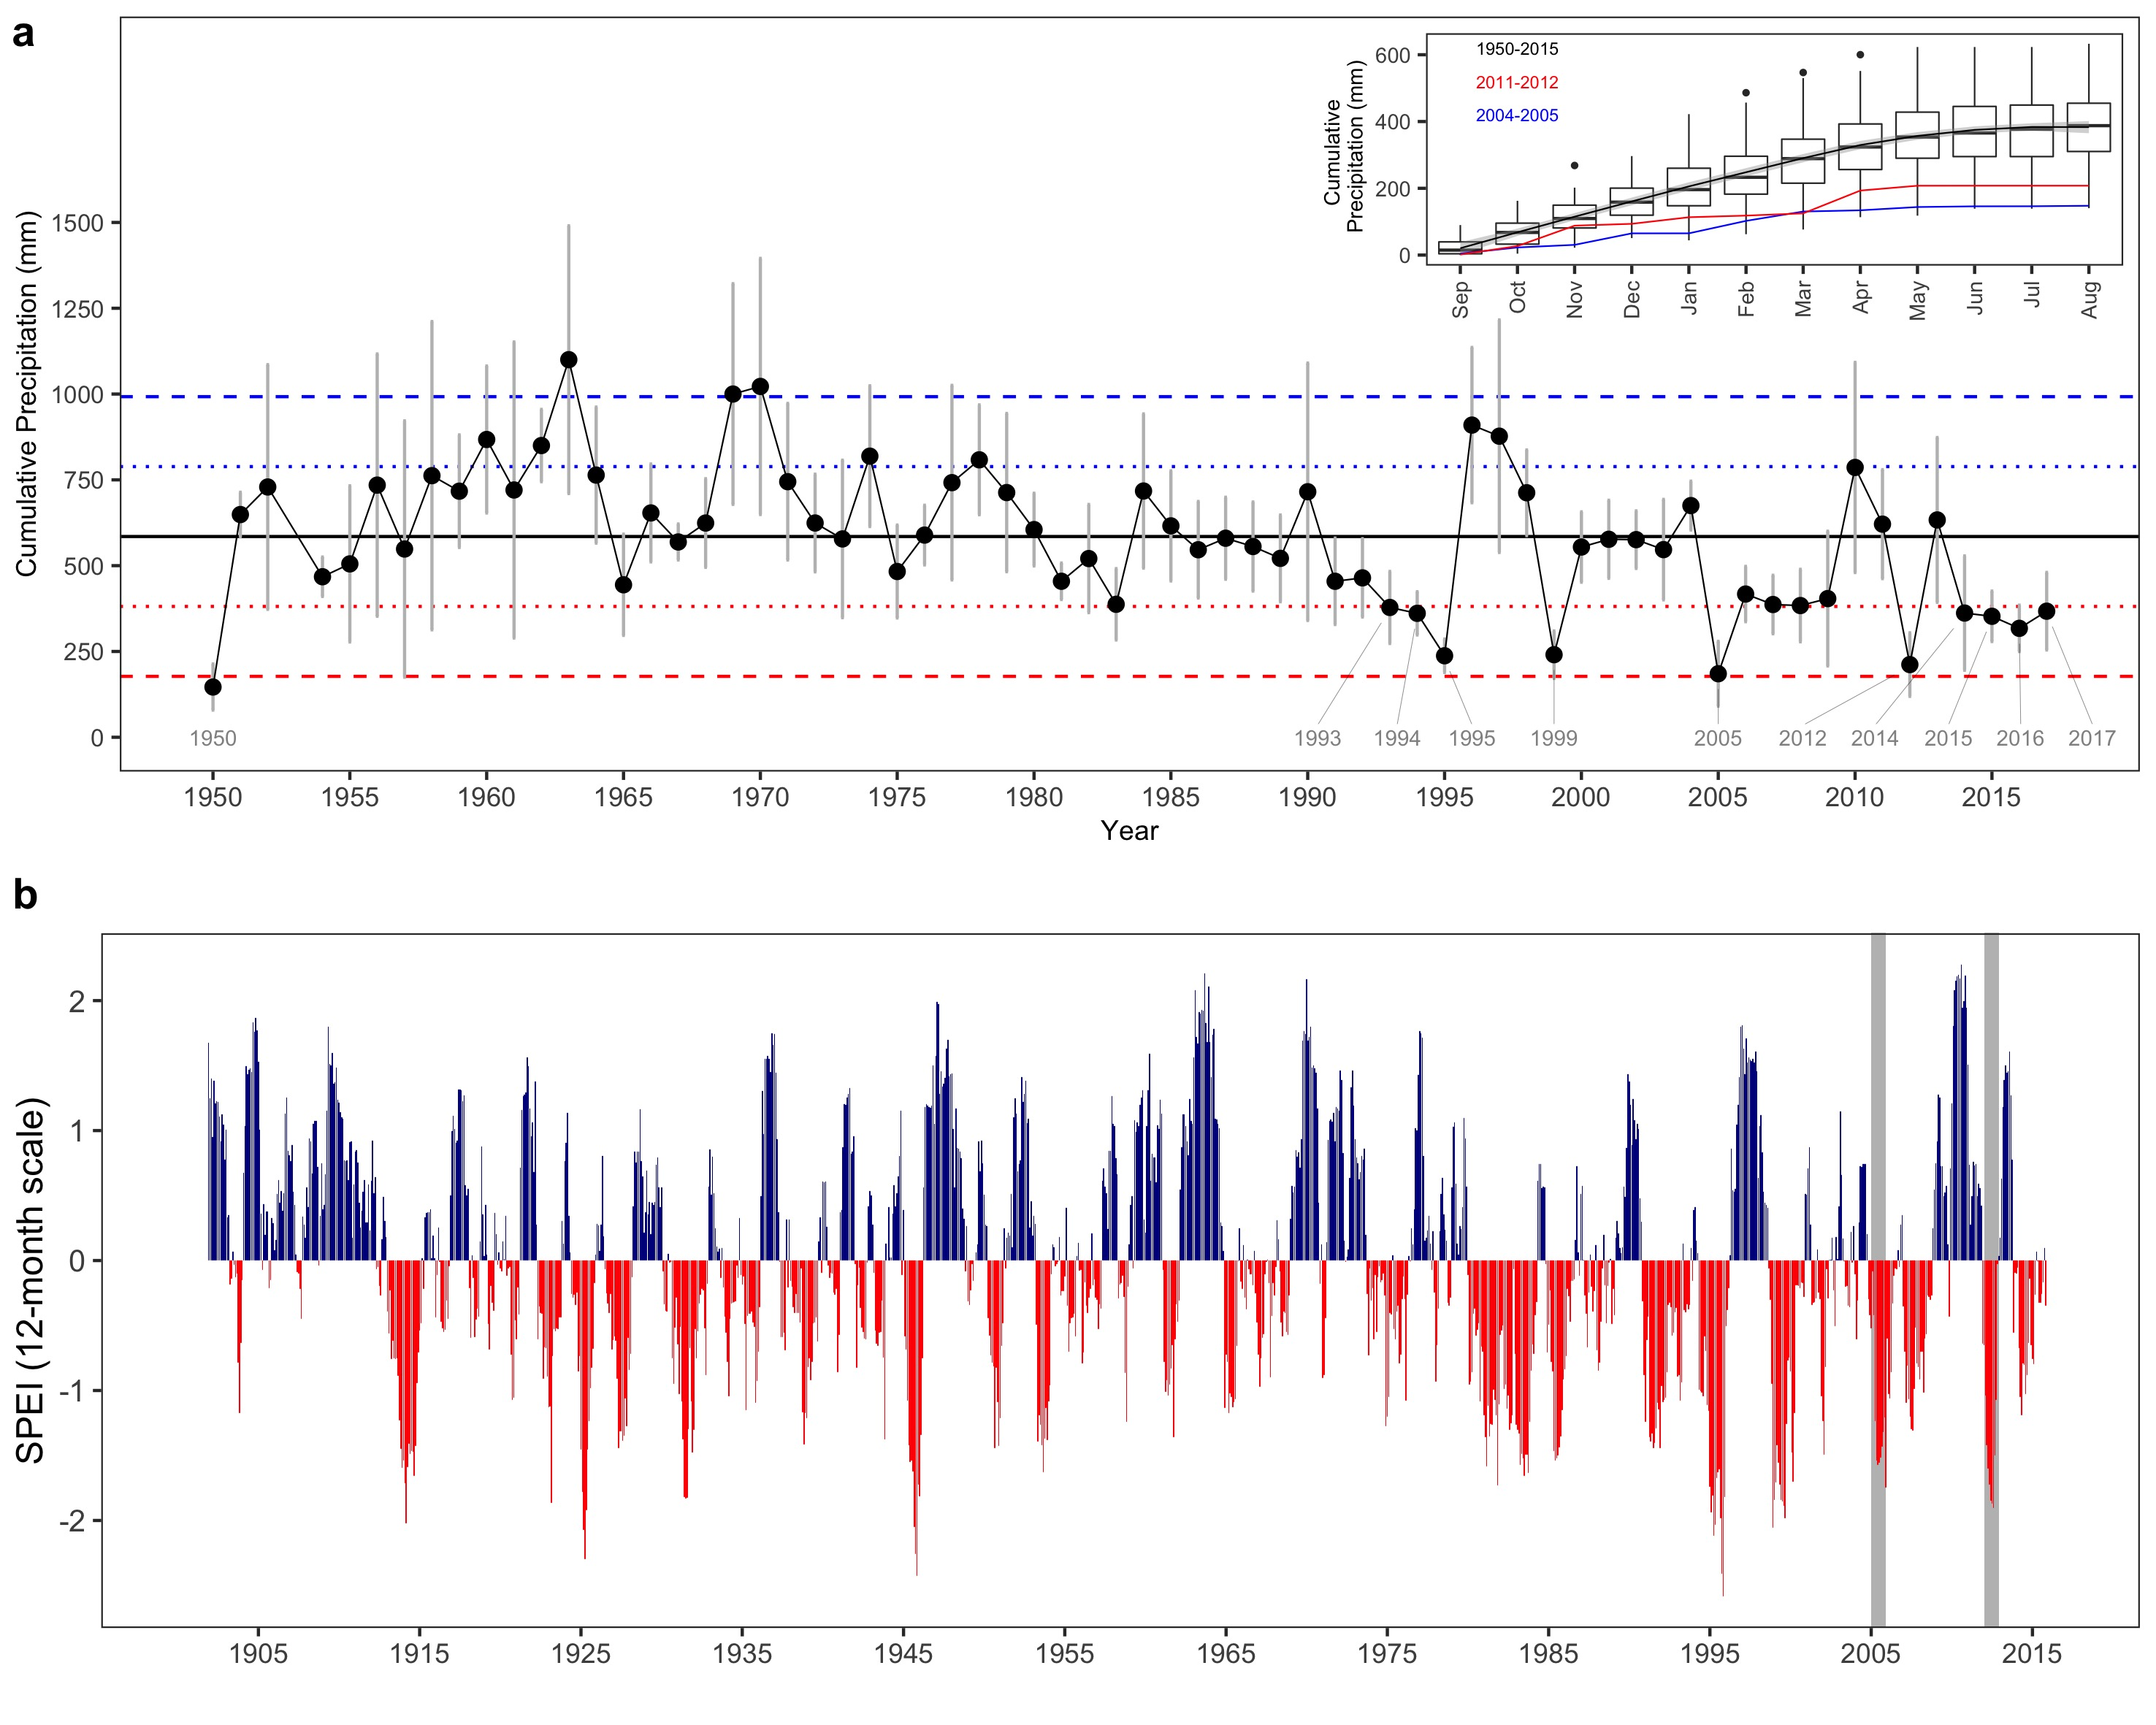
\includegraphics[width=\textwidth]{img/dendro/dendro-s1climate} 
\caption{\textbf{a)} Temporal evolution of cumulative precipitation (hydrological year) during the period 1950-2017. Points represent the mean, and error bars the standard error. The black line indicates mean for the entire period (585 mm). The red lines represent -1 and -2 standard deviation (dotted and dashed lines, respectively). The blue lines represent +1 and +2 standard deviation (dotted and dashed lines, respectively). Years with average values below -1SD are labeled. Data from 28 meteorological stations distributed around the Sierra Nevada area (from the National Spanish Meteorological Services, AEMET). Inset plot: cumulative precipitation during the hydrological years 2004-2005 (blue line) and 2011-2012 (red line). The boxplot representing the average from 1950-2015 period. Data from meteorological station Granada, Base Aérea. \textbf{b)} Drought severity in Sierra Nevada for the 1901-2016 period based on the Standardized Precipitation-Evapotranspiration Index (SPEI). Data from Global SPEI database (http://spei.csic.es/database.html). We took the SPEI data for a 12-month scale and for all 0.5\textdegree grid cells covering Sierra Nevada. Horizontal gray bars indicate the years 2005 and 2012.}  
\label{fig:dendro:s1climate}
\end{figure}
\newpage


\begin{figure}
\centering
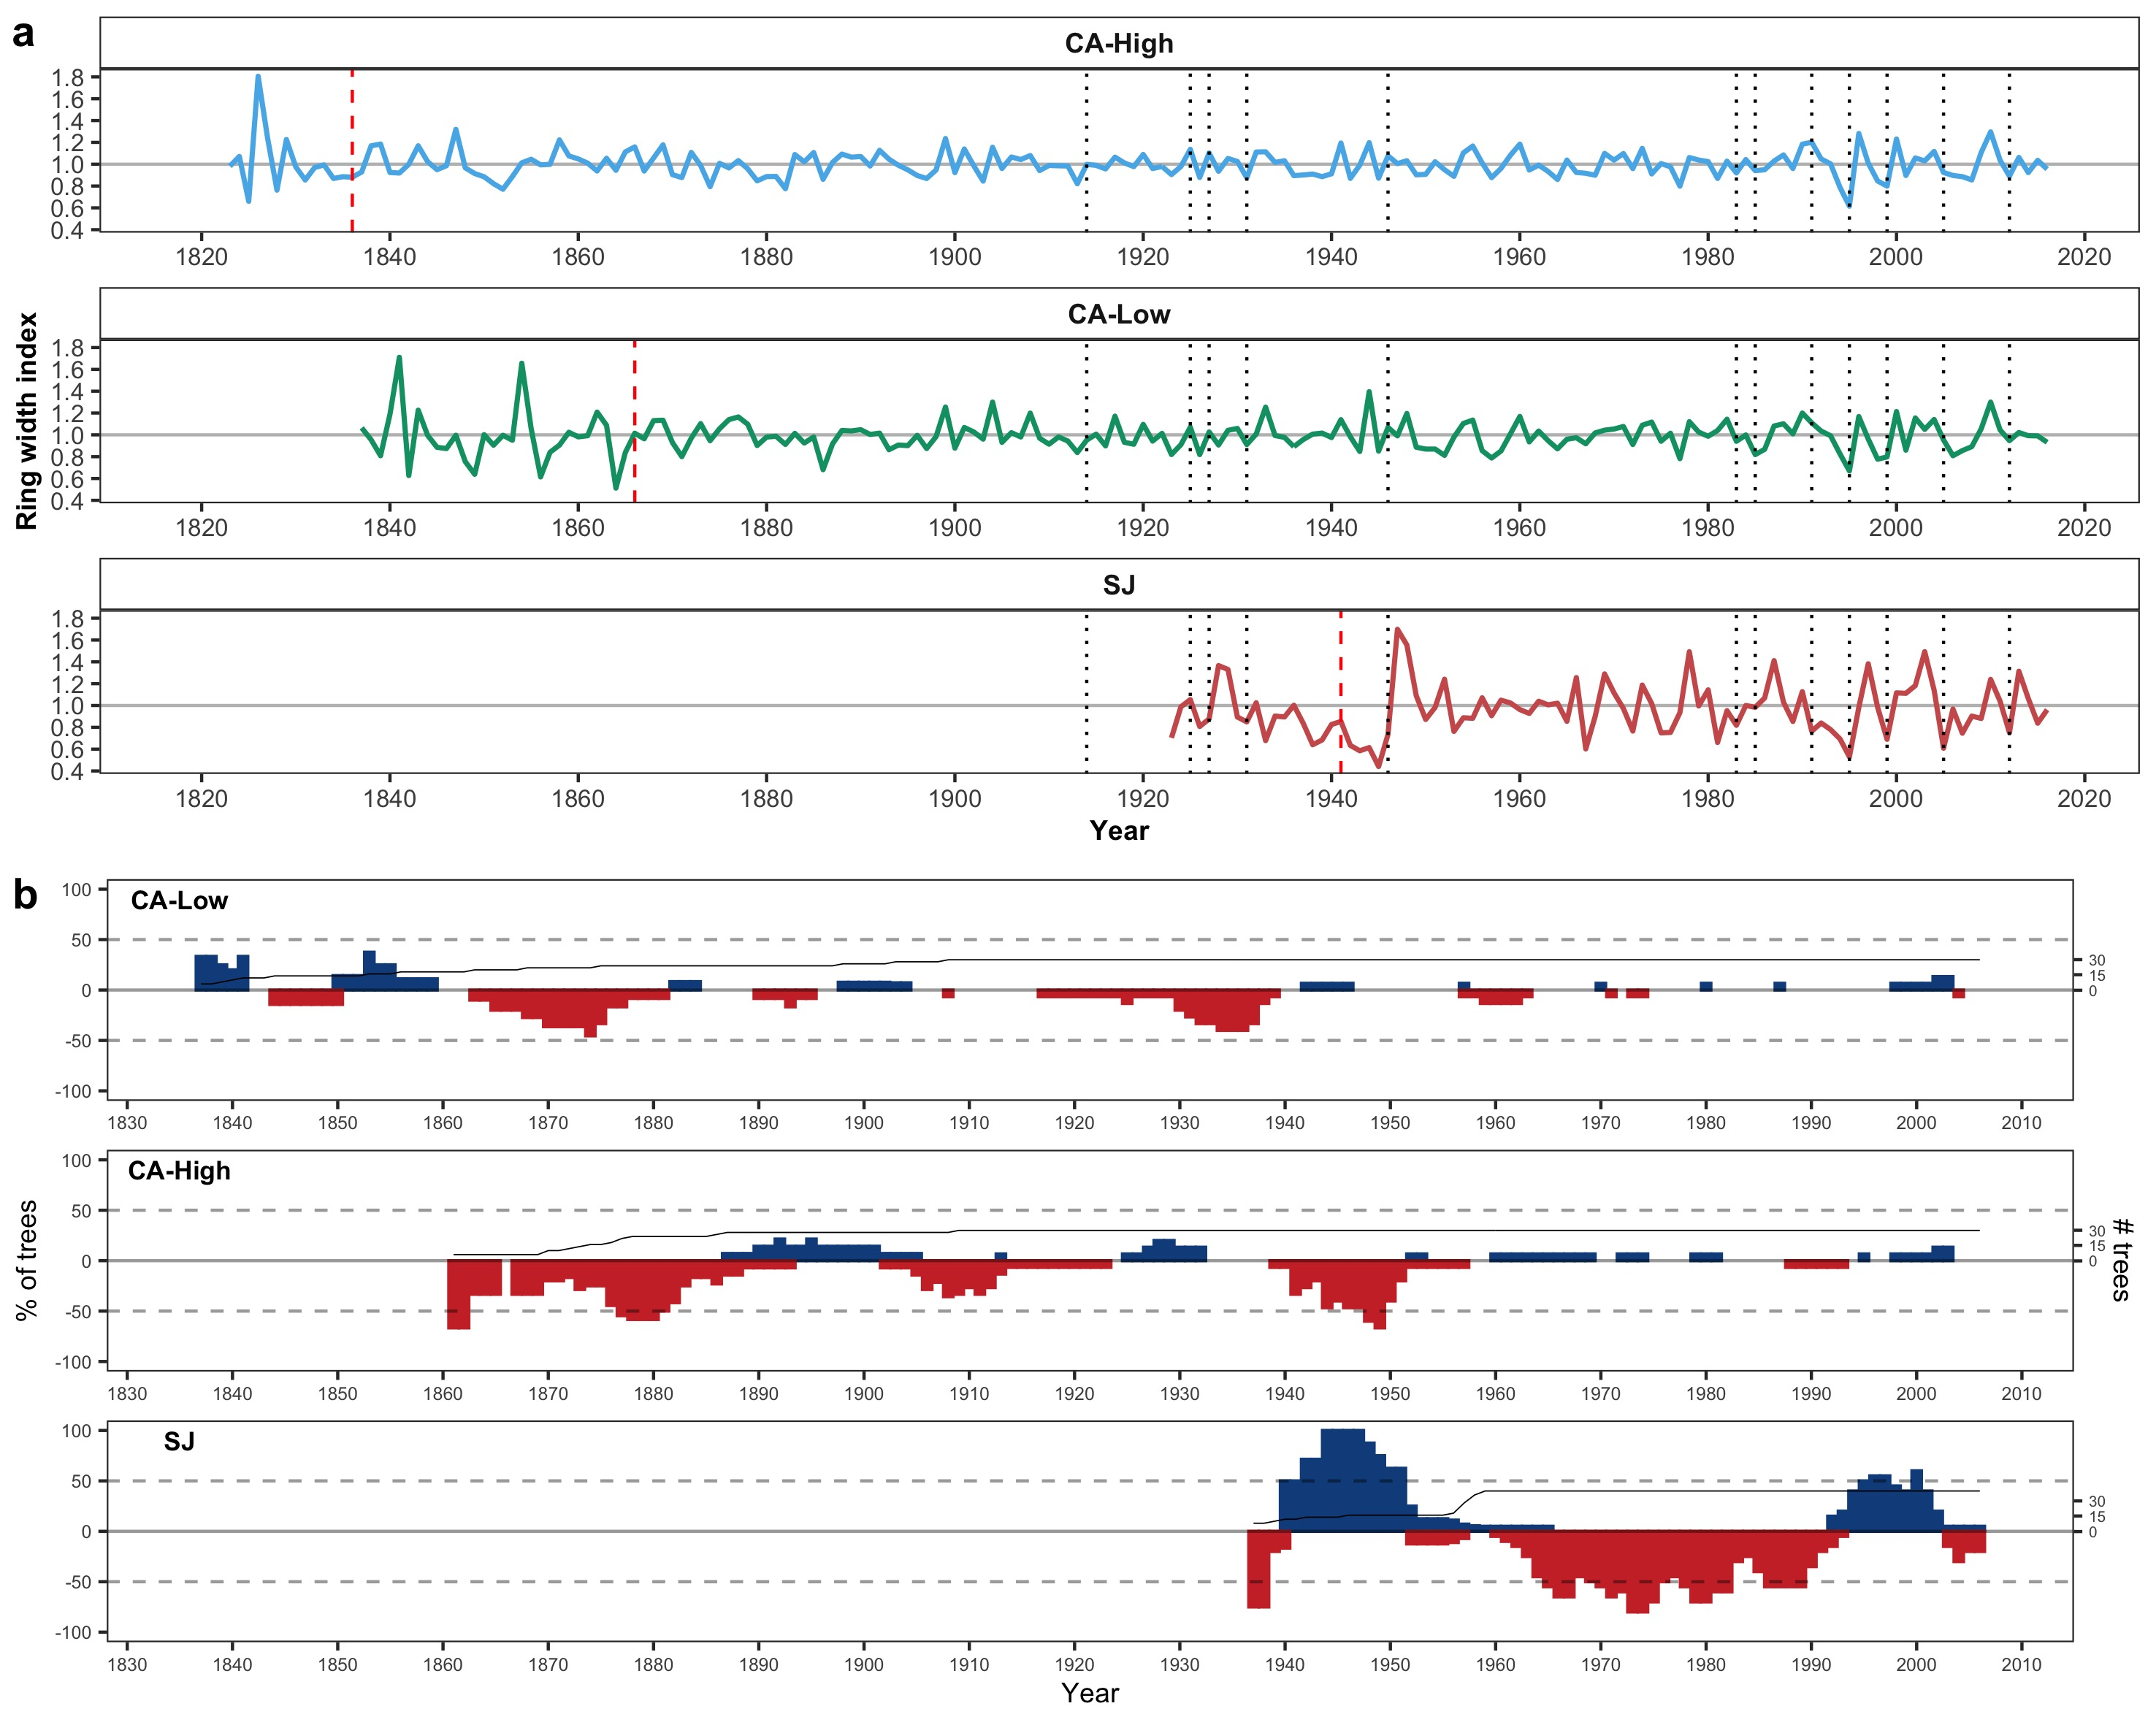
\includegraphics[width=\textwidth]{img/dendro/dendro-s2chronos} 
\caption{\textbf{a)} Residual tree-ring chronologies determined for the \Qp sites. Dashed red lines indicate the start of the reliable period (EPS > 0.85). Dotted black lines show the severe drought years identified in our climatic data (Table S3 and Figure S1). b) Percentage of \Qp trees affected by GC > 50 \% by site. Black line shows number of trees (right-axis). Data for number of trees > 2 is shown.
}  
\label{fig:dendro:s2chronos}
\end{figure}

\newpage
\begin{figure}
\centering
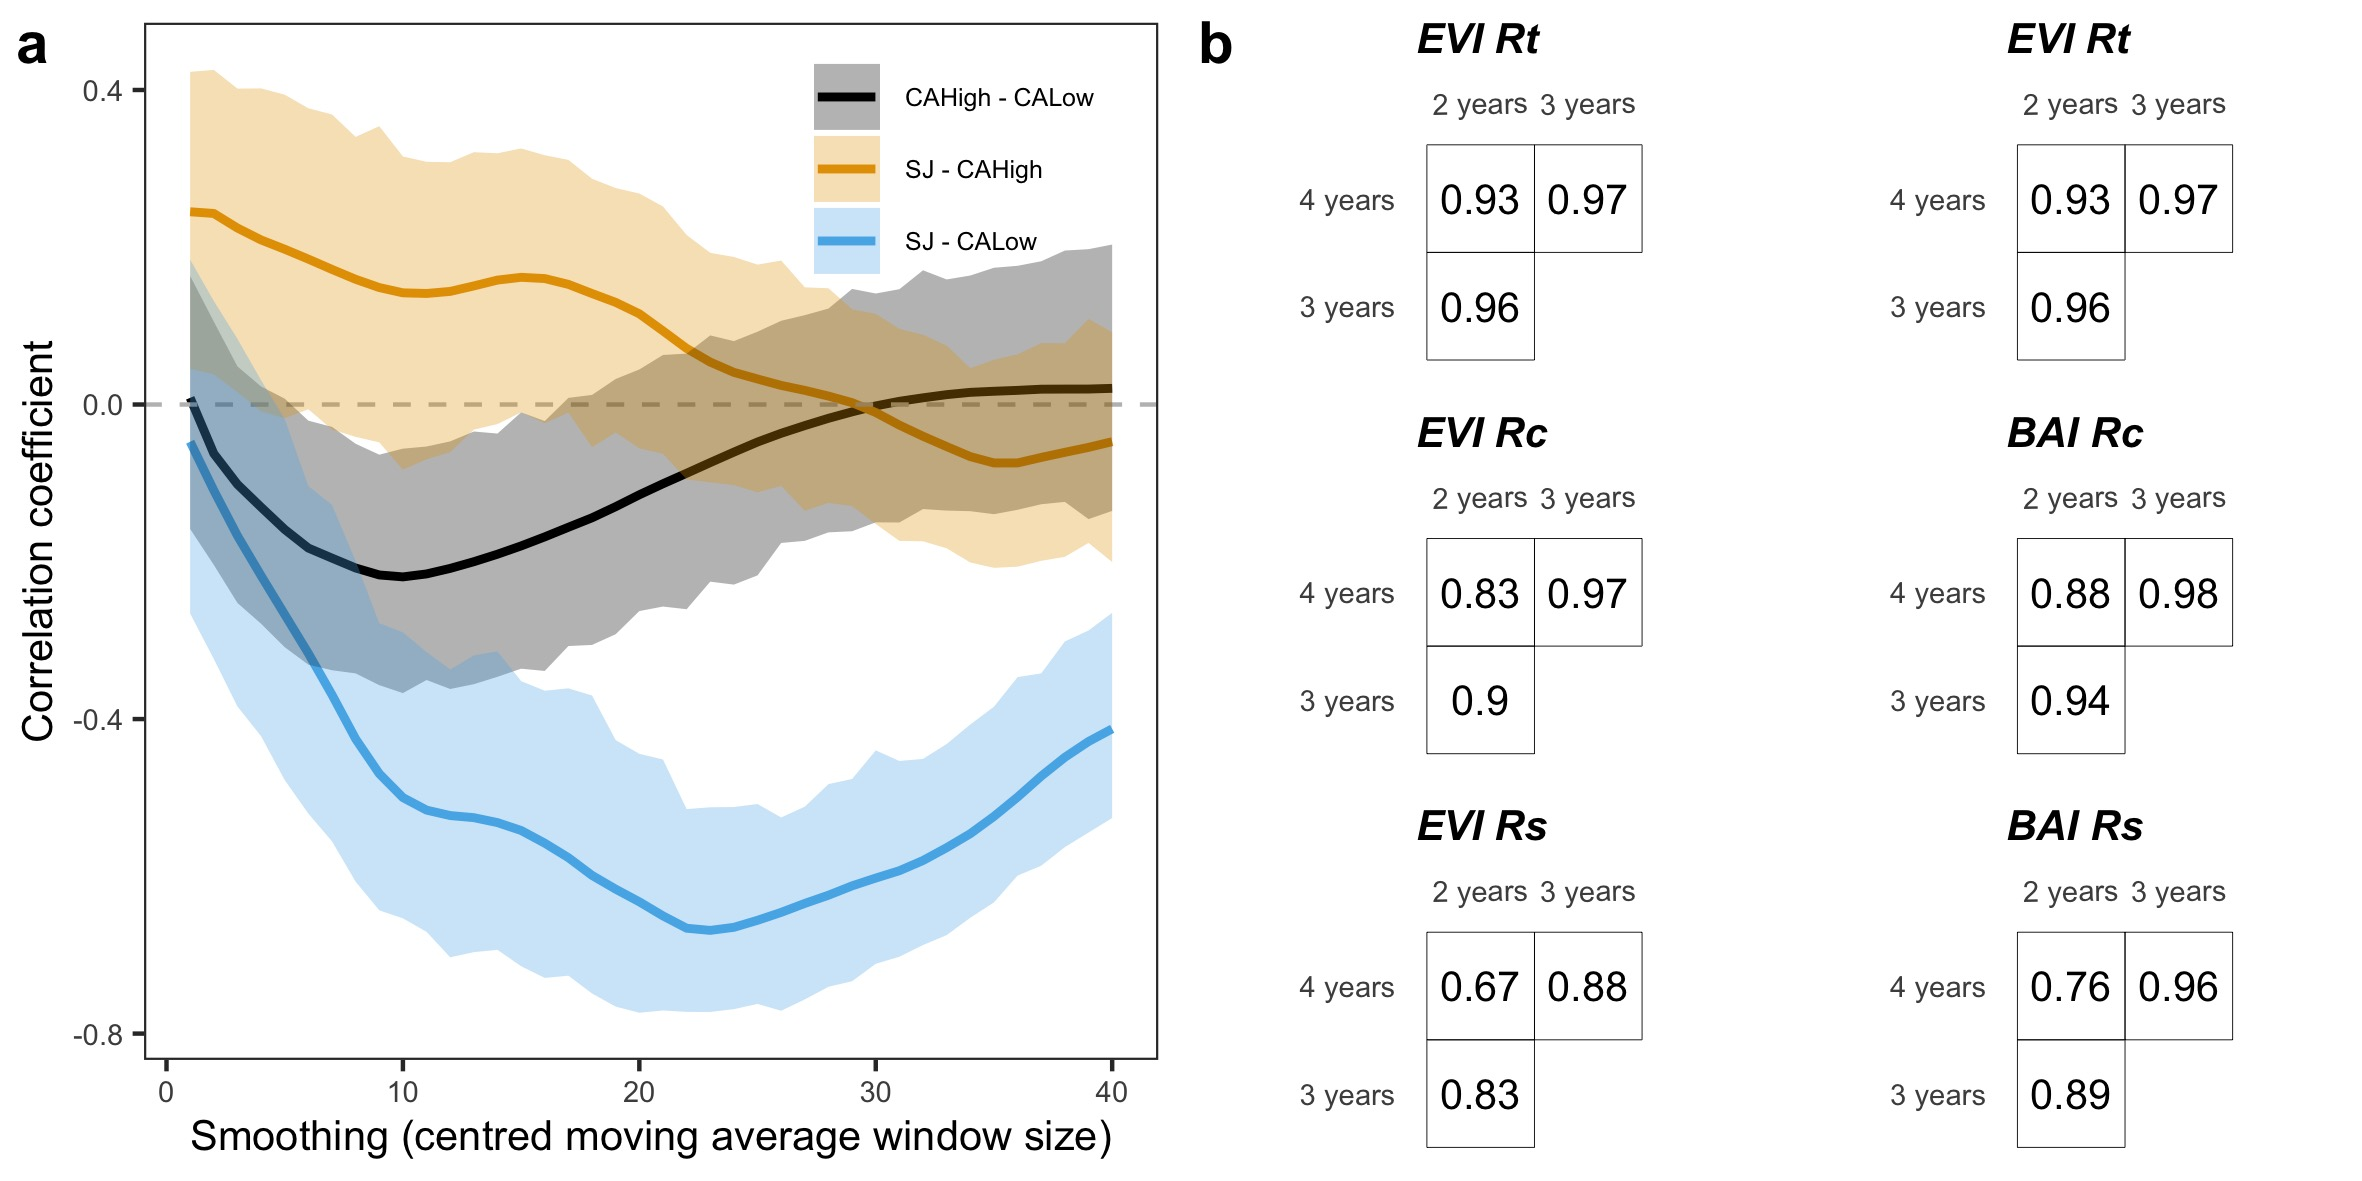
\includegraphics[width=\textwidth]{img/dendro/dendro-s3correlation} 
\caption{\textbf{a)} Correlation among site chronologies (CA-High, CA-Low and SJ) in different time domains after pre-filtering the time series with increasing size of the moving-average window (1 to 40 years). Each site chronology was smoothed using centered moving averages with different window sizes (1 to 40 years), and then Pearson’s correlation coefficient between the each pair of chronologies was calculated. Significance was tested using 1000 bootstrap replicates and with 95\% confidence intervals built using the R package boot. \textbf{b)} Correlation between indices of resilience (\emph{Rt}, resistance; \emph{Rc}, recovery; \emph{Rs}, Resilience) using periods of several lengths (2, 3 and 4 years after a drought).}  
\label{fig:dendro:s3correlations}
\end{figure}

\newpage
\begin{figure}
\centering
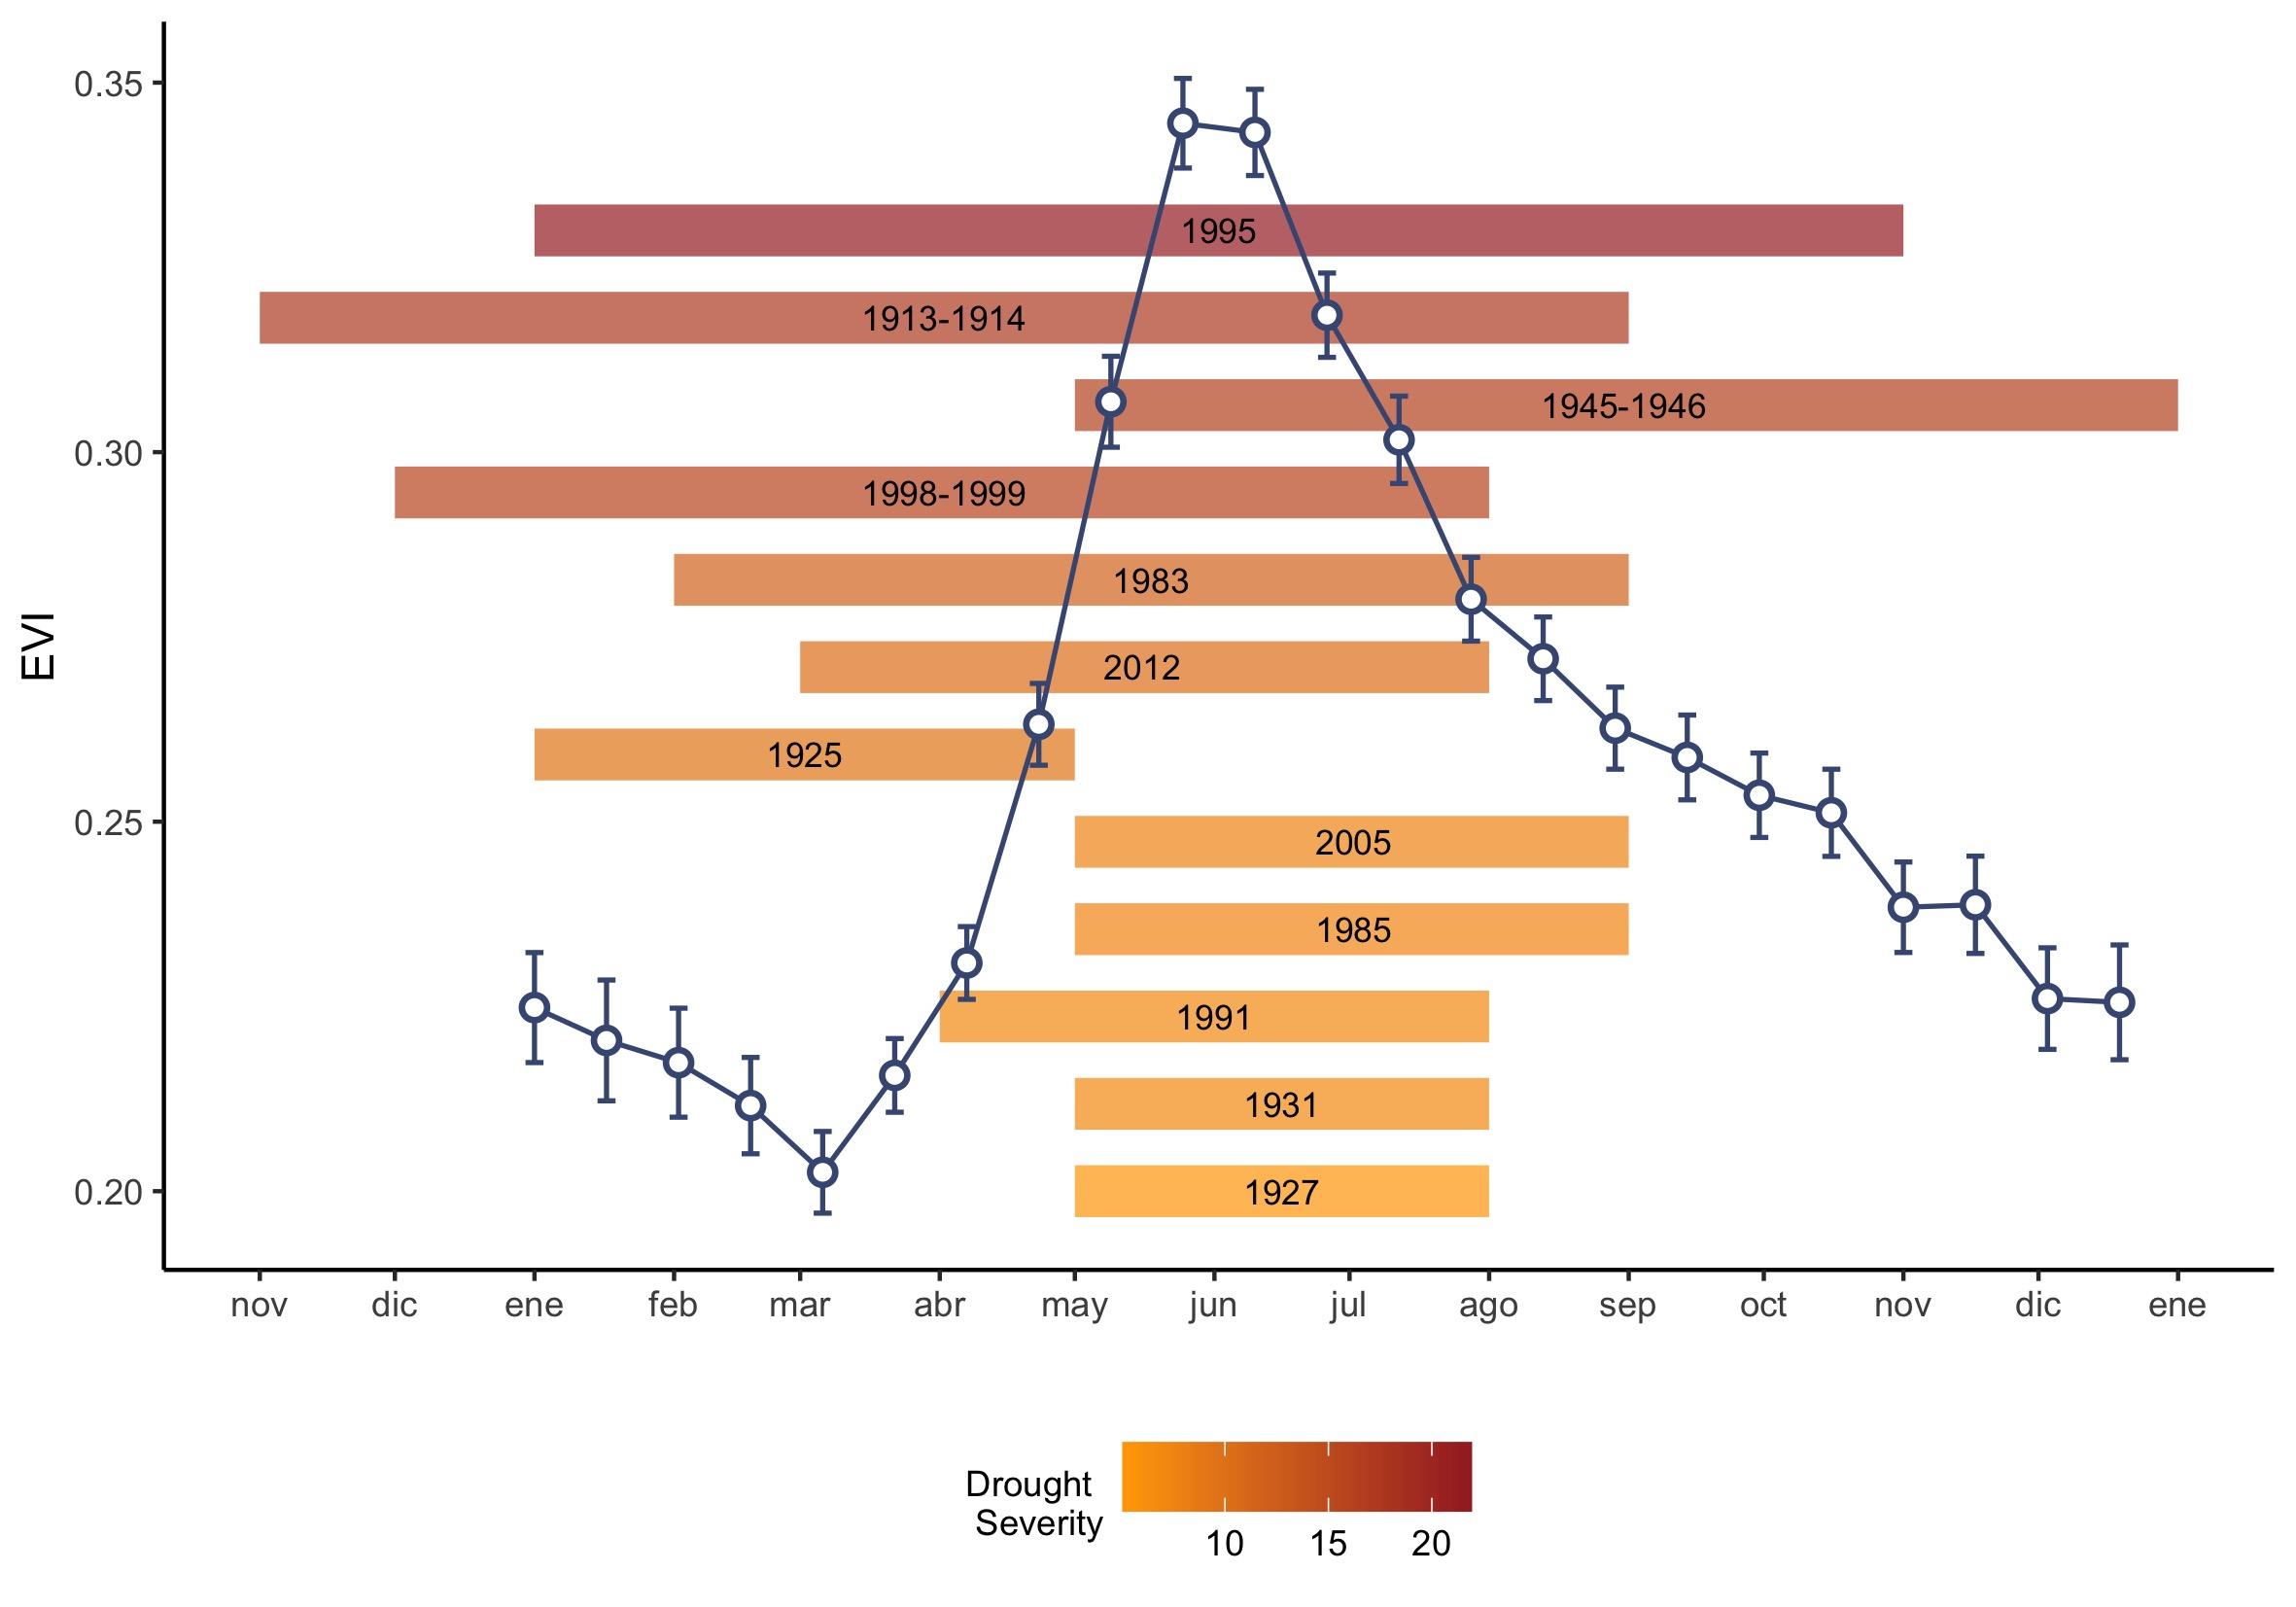
\includegraphics[width=\textwidth]{img/dendro/dendro-s4profile} 
\caption{EVI annual profile (average of the period 2000-2016) for \Qp forests in Sierra Nevada and drought events. Horizontal bars correspond to the most severe droughts for Sierra Nevada since 1900 (computed as in Table S3). Their position indicates the start and end months of each drought event. Bars lengths show the duration of the drought event \autocite[number of consecutive months with SPEI lower than -1.28, see][]{Pascoaetal2017DroughtTrends}.}  
\label{fig:dendro:s4profile}
\end{figure}

\newpage
\begin{figure}
\centering
\includegraphics[width=\textwidth]{img/dendro/dendro-s5resilience.jpg} 
\caption{Resilience metrics of the tree growth for severe drought events since 1950 (excluding 1995 drought event). Left: Resistance; Center: Recovery; Right: Resilience. Points indicate resilience metrics for oak populations: SJ (blue), CA-High (red) and CA-Low (green). Resilience metrics were computed for each population (sample depth > 10) and drought event. The gray line represents overall relationship for each Resilience metrics.}  
\label{fig:dendro:s5resilience}
\end{figure}

\newpage
\begin{figure}
\centering
\includegraphics[width=\textwidth]{img/dendro/dendro-s6corclimate.jpg} 
\caption{Correlation coefficients found by relating tree-ring residual chronologies (RWI) of \Qp and monthly climatic data: precipitation and 6-month SPEI \textbf{(a)}, minimum \textbf{(b)} and maximum \textbf{(c)} temperatures. green bars: northern site (SJ); light blue bars: low-elevation southern site (CA-Low); and dark blue bars: high-elevation southern site (CA-High). Asterisks indicate significant (\(p<0.05)\) correlation coefficients.}  
\label{fig:dendro:s6corclimate}
\end{figure}
       % INCLUDE: appendix

\cleardoublepage
% !TEX root = ../my-thesis.tex
%
\pagestyle{empty}
\hfill
\vfill
\pdfbookmark[0]{Colophon}{Colophon}
\section*{Colophon}

This thesis was typeset with \LaTeXe.
It uses the \textit{Clean Thesis} style developed by Ricardo Langner.
The design of the \textit{Clean Thesis} style is inspired by user guide documents from Apple Inc.

Download the \textit{Clean Thesis} style at \url{http://cleanthesis.der-ric.de/}.



\newpage
\mbox{}

% **************************************************
% End of Document CONTENT
% **************************************************
\end{document}
